\documentclass[twoside,11pt]{article}
\usepackage{layout}
% \usepackage{showframe}
\usepackage{blindtext}
% Any additional packages needeåd should be included after jmlr2e.
% Note that jmlr2e.sty includes epsfig, amssymb, natbib and graphicx,
% and defines many common macros, such as 'proof' and 'example'.
%
% It also sets the bibliographystyle to plainnat; for more information on
% natbib citation styles, see the natbib documentation, a copy of which
% is archived at http://www.jmlr.org/format/natbib.pdf

% Available options for package jmlr2e are:
%
%   - abbrvbib : use abbrvnat for the bibliography style
%   - nohyperref : do not load the hyperref package
%   - preprint : remove JMLR specific information from the template,
%         useful for example for posting to preprint servers.
%
% Example of using the package with custom options:
%
\usepackage[abbrvbib, preprint]{JMLR/jmlr2e_tight}

% \usepackage{JMLR/jmlr2e}

% Definitions of handy macros can go here

\newcommand{\dataset}{{\cal D}}
\newcommand{\fracpartial}[2]{\frac{\partial #1}{\partial  #2}}

% Heading arguments are {volume}{year}{pages}{date submitted}{date published}{paper id}{author-full-names}

\usepackage{lastpage}
\jmlrheading{23}{2022}{1-\pageref{LastPage}}{1/21; Revised 5/22}{9/22}{21-0000}{Author One and Author Two}

% Short headings should be running head and authors last names

\ShortHeadings{Risk Bounds for Quantile Temporal-Spatial Analysis}{Risk Bounds for Quantile Temporal-Spatial Analysis}
\firstpageno{1}


%%%% my own packages


\usepackage[utf8]{inputenc} % allow utf-8 input
\usepackage[T1]{fontenc}    % use 8-bit T1 fonts
\usepackage{microtype}
\emergencystretch=2em
\tolerance=1500
\overfullrule=5pt
\usepackage{graphicx}
% \usepackage{subfigure}
\usepackage{booktabs} % for professional tables
\usepackage{pgfplots}
\usepgfplotslibrary{groupplots}
\usepackage{pifont}
\newcommand\argument[1]{\mathtt{#1}}
\newcommand\constraint[1]{\textsc{#1}}
\usepackage{hyperref}
\usepackage{stmaryrd}
\usepackage{algorithmic}
\usepackage[ruled,vlined]{algorithm2e}
% Attempt to make hyperref and algorithmic work together better:
\newcommand{\theHalgorithm}{\arabic{algorithm}}

% Use the following line for the initial blind version submitted for review:

% \def\baselinestretch{0.99}
% If accepted, instead use the following line for the camera-ready submission:
% \usepackage[accepted]{icml2023}

% For theorems and such
% \usepackage{amsmath}
\usepackage{amssymb}
\usepackage{bbm}
\usepackage{mathtools}
% \usepackage{amsthm}
\usepackage{multicol}
% if you use cleveref..
\usepackage[capitalize,noabbrev]{cleveref}

\usepackage{xcolor}
\definecolor{orange}{rgb}{0.2,0.7,0.4}

% \usepackage[utf8]{inputenc} % allow utf-8 input
% \usepackage[T1]{fontenc}    % use 8-bit T1 fonts

% Recommended, but optional, packages for figures and better typesetting:
% \usepackage[FIGTOPCAP]{subfigure}% note: subfigure and subcaption can't be used together



\usepackage{graphicx}
\usepackage{wrapfig}
\graphicspath{{figures/}}%set the relative figure path 
\usepackage{caption}
% \captionsetup{font=small}
\usepackage{subcaption}
\captionsetup{font=normalsize,labelfont={bf,sf}}
\captionsetup[sub]{font=small,labelfont={bf,sf}}


\usepackage{amsfonts}
\usepackage{mwe}
\usepackage{multirow}
\newlength{\tempheight}
\newlength{\tempwidth}

\newcommand{\step}[1]{\par\medskip\noindent\textbf{#1.}\ }

\usepackage{enumitem}
\setlist[enumerate,1]{label={\bfseries\arabic*.},ref={\bfseries\theenumii.\arabic*}}
\setlist[enumerate,2]{label={\bfseries\alph*)},ref={\bfseries\theenumi\alph*)}}
\usepackage{makecell}

\usepackage{tabularx}
\usepackage{float}

\usepackage{pgfplots}


% \usepackage{titlesec}
% \titlespacing\section{0pt}{2pt plus 4pt minus 6pt}{0pt plus 4pt minus 6pt}
% \titlespacing\subsection{0pt}{2pt plus 4pt minus 6pt}{0pt plus 4pt minus 6pt}
% \titlespacing\subsubsection{0pt}{12pt plus 4pt minus 2pt}{0pt plus 2pt minus 2pt}

% Todonotes is useful during development; simply uncomment the next line
%    and comment out the line below the next line to turn off comments
% \usepackage[disable,textsize=tiny]{todonotes}
% \usepackage[textsize=tiny]{todonotes}
%%%%% NEW MATH DEFINITIONS %%%%%

\usepackage{amsmath,amsfonts,bm,mathrsfs}
% \RequirePackage{algorithm}
% \RequirePackage{algorithmic}
% Mark sections of captions for referring to divisions of figures
\newcommand{\figleft}{{\em (Left)}}
\newcommand{\figcenter}{{\em (Center)}}
\newcommand{\figright}{{\em (Right)}}
\newcommand{\figtop}{{\em (Top)}}
\newcommand{\figbottom}{{\em (Bottom)}}
\newcommand{\captiona}{{\em (a)}}
\newcommand{\captionb}{{\em (b)}}
\newcommand{\captionc}{{\em (c)}}
\newcommand{\captiond}{{\em (d)}}

% Highlight a newly defined term
\newcommand{\newterm}[1]{{\bf #1}}


% Figure reference, lower-case.
\def\figref#1{figure~\ref{#1}}
% Figure reference, capital. For start of sentence
\def\Figref#1{Figure~\ref{#1}}
\def\twofigref#1#2{figures \ref{#1} and \ref{#2}}
\def\quadfigref#1#2#3#4{figures \ref{#1}, \ref{#2}, \ref{#3} and \ref{#4}}
% Section reference, lower-case.
\def\secref#1{section~\ref{#1}}
% Section reference, capital.
\def\Secref#1{Section~\ref{#1}}
% Reference to two sections.
\def\twosecrefs#1#2{sections \ref{#1} and \ref{#2}}
% Reference to three sections.
\def\secrefs#1#2#3{sections \ref{#1}, \ref{#2} and \ref{#3}}
% Reference to an equation, lower-case.
\def\eqrefe#1{equation~\ref{#1}}
% Reference to an equation, upper case
\def\Eqref#1{Equation~\ref{#1}}
% A raw reference to an equation---avoid using if possible
\def\plaineqref#1{\ref{#1}}
% Reference to a chapter, lower-case.
\def\chapref#1{chapter~\ref{#1}}
% Reference to an equation, upper case.
\def\Chapref#1{Chapter~\ref{#1}}
% Reference to a range of chapters
\def\rangechapref#1#2{chapters\ref{#1}--\ref{#2}}
% Reference to an algorithm, lower-case.
\def\algref#1{algorithm~\ref{#1}}
% Reference to an algorithm, upper case.
\def\Algref#1{Algorithm~\ref{#1}}
\def\twoalgref#1#2{algorithms \ref{#1} and \ref{#2}}
\def\Twoalgref#1#2{Algorithms \ref{#1} and \ref{#2}}
% Reference to a part, lower case
\def\partref#1{part~\ref{#1}}
% Reference to a part, upper case
\def\Partref#1{Part~\ref{#1}}
\def\twopartref#1#2{parts \ref{#1} and \ref{#2}}

% \def\ceil#1{\lceil #1 \rceil}
\newcommand{\ceil}[1]{{\left\lceil{#1}\right\rceil}}

% \def\floor#1{\lfloor #1 \rfloor}
\newcommand{\floor}[1]{{\left\lfloor{#1}\right\rfloor}}

\def\1{\bm{1}}
\newcommand{\train}{\mathcal{D}}
\newcommand{\valid}{\mathcal{D_{\mathrm{valid}}}}
\newcommand{\test}{\mathcal{D_{\mathrm{test}}}}

\def\eps{{\epsilon}}
% \newcommand{\eps}{\varepsilon}

% Random variables
\def\reta{{\textnormal{$\eta$}}}
\def\ra{{\textnormal{a}}}
\def\rb{{\textnormal{b}}}
\def\rc{{\textnormal{c}}}
\def\rd{{\textnormal{d}}}
\def\re{{\textnormal{e}}}
\def\rf{{\textnormal{f}}}
\def\rg{{\textnormal{g}}}
\def\rh{{\textnormal{h}}}
\def\ri{{\textnormal{i}}}
\def\rj{{\textnormal{j}}}
\def\rk{{\textnormal{k}}}
\def\rl{{\textnormal{l}}}
% rm is already a command, just don't name any random variables m
\def\rn{{\textnormal{n}}}
\def\ro{{\textnormal{o}}}
\def\rp{{\textnormal{p}}}
\def\rq{{\textnormal{q}}}
\def\rr{{\textnormal{r}}}
\def\rs{{\textnormal{s}}}
\def\rt{{\textnormal{t}}}
\def\ru{{\textnormal{u}}}
\def\rv{{\textnormal{v}}}
\def\rw{{\textnormal{w}}}
\def\rx{{\textnormal{x}}}
\def\ry{{\textnormal{y}}}
\def\rz{{\textnormal{z}}}

% Random vectors
\def\rvepsilon{{\mathbf{\epsilon}}}
\def\rvtheta{{\mathbf{\theta}}}
\def\rva{{\mathbf{a}}}
\def\rvb{{\mathbf{b}}}
\def\rvc{{\mathbf{c}}}
\def\rvd{{\mathbf{d}}}
\def\rve{{\mathbf{e}}}
\def\rvf{{\mathbf{f}}}
\def\rvg{{\mathbf{g}}}
\def\rvh{{\mathbf{h}}}
\def\rvi{{\mathbf{i}}}
\def\rvj{{\mathbf{j}}}
\def\rvk{{\mathbf{k}}}
\def\rvl{{\mathbf{l}}}
\def\rvm{{\mathbf{m}}}
\def\rvn{{\mathbf{n}}}
\def\rvo{{\mathbf{o}}}
\def\rvp{{\mathbf{p}}}
\def\rvq{{\mathbf{q}}}
\def\rvr{{\mathbf{r}}}
\def\rvs{{\mathbf{s}}}
\def\rvt{{\mathbf{t}}}
\def\rvu{{\mathbf{u}}}
\def\rvv{{\mathbf{v}}}
\def\rvw{{\mathbf{w}}}
\def\rvx{{\mathbf{x}}}
\def\rvy{{\mathbf{y}}}
\def\rvz{{\mathbf{z}}}
\def\rvone{{\mathbf{1}}}
\def\rvzero{{\mathbf{0}}}

% Elements of random vectors
\def\erva{{\textnormal{a}}}
\def\ervb{{\textnormal{b}}}
\def\ervc{{\textnormal{c}}}
\def\ervd{{\textnormal{d}}}
\def\erve{{\textnormal{e}}}
\def\ervf{{\textnormal{f}}}
\def\ervg{{\textnormal{g}}}
\def\ervh{{\textnormal{h}}}
\def\ervi{{\textnormal{i}}}
\def\ervj{{\textnormal{j}}}
\def\ervk{{\textnormal{k}}}
\def\ervl{{\textnormal{l}}}
\def\ervm{{\textnormal{m}}}
\def\ervn{{\textnormal{n}}}
\def\ervo{{\textnormal{o}}}
\def\ervp{{\textnormal{p}}}
\def\ervq{{\textnormal{q}}}
\def\ervr{{\textnormal{r}}}
\def\ervs{{\textnormal{s}}}
\def\ervt{{\textnormal{t}}}
\def\ervu{{\textnormal{u}}}
\def\ervv{{\textnormal{v}}}
\def\ervw{{\textnormal{w}}}
\def\ervx{{\textnormal{x}}}
\def\ervy{{\textnormal{y}}}
\def\ervz{{\textnormal{z}}}

% Random matrices
\def\rmA{{\mathbf{A}}}
\def\rmB{{\mathbf{B}}}
\def\rmC{{\mathbf{C}}}
\def\rmD{{\mathbf{D}}}
\def\rmE{{\mathbf{E}}}
\def\rmF{{\mathbf{F}}}
\def\rmG{{\mathbf{G}}}
\def\rmH{{\mathbf{H}}}
\def\rmI{{\mathbf{I}}}
\def\rmJ{{\mathbf{J}}}
\def\rmK{{\mathbf{K}}}
\def\rmL{{\mathbf{L}}}
\def\rmM{{\mathbf{M}}}
\def\rmN{{\mathbf{N}}}
\def\rmO{{\mathbf{O}}}
\def\rmP{{\mathbf{P}}}
\def\rmQ{{\mathbf{Q}}}
\def\rmR{{\mathbf{R}}}
\def\rmS{{\mathbf{S}}}
\def\rmT{{\mathbf{T}}}
\def\rmU{{\mathbf{U}}}
\def\rmV{{\mathbf{V}}}
\def\rmW{{\mathbf{W}}}
\def\rmX{{\mathbf{X}}}
\def\rmY{{\mathbf{Y}}}
\def\rmZ{{\mathbf{Z}}}

% Elements of random matrices
\def\ermA{{\textnormal{A}}}
\def\ermB{{\textnormal{B}}}
\def\ermC{{\textnormal{C}}}
\def\ermD{{\textnormal{D}}}
\def\ermE{{\textnormal{E}}}
\def\ermF{{\textnormal{F}}}
\def\ermG{{\textnormal{G}}}
\def\ermH{{\textnormal{H}}}
\def\ermI{{\textnormal{I}}}
\def\ermJ{{\textnormal{J}}}
\def\ermK{{\textnormal{K}}}
\def\ermL{{\textnormal{L}}}
\def\ermM{{\textnormal{M}}}
\def\ermN{{\textnormal{N}}}
\def\ermO{{\textnormal{O}}}
\def\ermP{{\textnormal{P}}}
\def\ermQ{{\textnormal{Q}}}
\def\ermR{{\textnormal{R}}}
\def\ermS{{\textnormal{S}}}
\def\ermT{{\textnormal{T}}}
\def\ermU{{\textnormal{U}}}
\def\ermV{{\textnormal{V}}}
\def\ermW{{\textnormal{W}}}
\def\ermX{{\textnormal{X}}}
\def\ermY{{\textnormal{Y}}}
\def\ermZ{{\textnormal{Z}}}

% Vectors
\def\vzero{{\bm{0}}}
\def\vone{{\bm{1}}}
\def\vmu{{\bm{\mu}}}
\def\vtheta{{\bm{\theta}}}
\def\va{{\bm{a}}}
\def\vb{{\bm{b}}}
\def\vc{{\bm{c}}}
\def\vd{{\bm{d}}}
\def\ve{{\bm{e}}}
\def\vf{{\bm{f}}}
\def\vg{{\bm{g}}}
\def\vh{{\bm{h}}}
\def\vi{{\bm{i}}}
\def\vj{{\bm{j}}}
\def\vk{{\bm{k}}}
\def\vl{{\bm{l}}}
\def\vm{{\bm{m}}}
\def\vn{{\bm{n}}}
\def\vo{{\bm{o}}}
\def\vp{{\bm{p}}}
\def\vq{{\bm{q}}}
\def\vr{{\bm{r}}}
\def\vs{{\bm{s}}}
\def\vt{{\bm{t}}}
\def\vu{{\bm{u}}}
\def\vv{{\bm{v}}}
\def\vw{{\bm{w}}}
\def\vx{{\bm{x}}}
\def\vy{{\bm{y}}}
\def\vz{{\bm{z}}}

% Elements of vectors
\def\evalpha{{\alpha}}
\def\evbeta{{\beta}}
\def\evepsilon{{\epsilon}}
\def\evlambda{{\lambda}}
\def\evomega{{\omega}}
\def\evmu{{\mu}}
\def\evpsi{{\psi}}
\def\evsigma{{\sigma}}
\def\evtheta{{\theta}}
\def\eva{{a}}
\def\evb{{b}}
\def\evc{{c}}
\def\evd{{d}}
\def\eve{{e}}
\def\evf{{f}}
\def\evg{{g}}
\def\evh{{h}}
\def\evi{{i}}
\def\evj{{j}}
\def\evk{{k}}
\def\evl{{l}}
\def\evm{{m}}
\def\evn{{n}}
\def\evo{{o}}
\def\evp{{p}}
\def\evq{{q}}
\def\evr{{r}}
\def\evs{{s}}
\def\evt{{t}}
\def\evu{{u}}
\def\evv{{v}}
\def\evw{{w}}
\def\evx{{x}}
\def\evy{{y}}
\def\evz{{z}}

% Matrix
\def\mA{{\bm{A}}}
\def\mB{{\bm{B}}}
\def\mC{{\bm{C}}}
\def\mD{{\bm{D}}}
\def\mE{{\bm{E}}}
\def\mF{{\bm{F}}}
\def\mG{{\bm{G}}}
\def\mH{{\bm{H}}}
\def\mI{{\bm{I}}}
\def\mJ{{\bm{J}}}
\def\mK{{\bm{K}}}
\def\mL{{\bm{L}}}
\def\mM{{\bm{M}}}
\def\mN{{\bm{N}}}
\def\mO{{\bm{O}}}
\def\mP{{\bm{P}}}
\def\mQ{{\bm{Q}}}
\def\mR{{\bm{R}}}
\def\mS{{\bm{S}}}
\def\mT{{\bm{T}}}
\def\mU{{\bm{U}}}
\def\mV{{\bm{V}}}
\def\mW{{\bm{W}}}
\def\mX{{\bm{X}}}
\def\mY{{\bm{Y}}}
\def\mZ{{\bm{Z}}}
\def\mBeta{{\bm{\beta}}}
\def\mPhi{{\bm{\Phi}}}
\def\mLambda{{\bm{\Lambda}}}
\def\mSigma{{\bm{\Sigma}}}

% Tensor
\DeclareMathAlphabet{\mathsfit}{\encodingdefault}{\sfdefault}{m}{sl}
\SetMathAlphabet{\mathsfit}{bold}{\encodingdefault}{\sfdefault}{bx}{n}
\newcommand{\tens}[1]{\bm{\mathsfit{#1}}}

% \NewDocumentCommand{\tens}{t_}
%  {%
%   \IfBooleanTF{#1}
%    {\tensop}
%    {\otimes}%
%  }
 
\def\tA{{\tens{A}}}
\def\tB{{\tens{B}}}
\def\tC{{\tens{C}}}
\def\tD{{\tens{D}}}
\def\tE{{\tens{E}}}
\def\tF{{\tens{F}}}
\def\tG{{\tens{G}}}
\def\tH{{\tens{H}}}
\def\tI{{\tens{I}}}
\def\tJ{{\tens{J}}}
\def\tK{{\tens{K}}}
\def\tL{{\tens{L}}}
\def\tM{{\tens{M}}}
\def\tN{{\tens{N}}}
\def\tO{{\tens{O}}}
\def\tP{{\tens{P}}}
\def\tQ{{\tens{Q}}}
\def\tR{{\tens{R}}}
\def\tS{{\tens{S}}}
\def\tT{{\tens{T}}}
\def\tU{{\tens{U}}}
\def\tV{{\tens{V}}}
\def\tW{{\tens{W}}}
\def\tX{{\tens{X}}}
\def\tY{{\tens{Y}}}
\def\tZ{{\tens{Z}}}


% 

\def\fX{{\mathfrak{X}}}
\def\fY{{\mathfrak{Y}}}

% Graph
\def\gA{{\mathcal{A}}}
\def\gB{{\mathcal{B}}}
\def\gC{{\mathcal{C}}}
\def\gD{{\mathcal{D}}}
\def\gE{{\mathcal{E}}}
\def\gF{{\mathcal{F}}}
\def\gG{{\mathcal{G}}}
\def\gH{{\mathcal{H}}}
\def\gI{{\mathcal{I}}}
\def\gJ{{\mathcal{J}}}
\def\gK{{\mathcal{K}}}
\def\gL{{\mathcal{L}}}
\def\gM{{\mathcal{M}}}
\def\gN{{\mathcal{N}}}
\def\gO{{\mathcal{O}}}
\def\gP{{\mathcal{P}}}
\def\gQ{{\mathcal{Q}}}
\def\gR{{\mathcal{R}}}
\def\gS{{\mathcal{S}}}
\def\gT{{\mathcal{T}}}
\def\gU{{\mathcal{U}}}
\def\gV{{\mathcal{V}}}
\def\gW{{\mathcal{W}}}
\def\gX{{\mathcal{X}}}
\def\gY{{\mathcal{Y}}}
\def\gZ{{\mathcal{Z}}}

\def\rS{{\mathscr{S}}}
\def\rA{{\mathscr{A}}}
\def\rB{{\mathscr{B}}}
\def\rC{{\mathscr{C}}}
\def\rD{{\mathscr{D}}}
\def\rE{{\mathscr{E}}}
\def\rF{{\mathscr{F}}}
\def\rG{{\mathscr{G}}}
\def\rH{{\mathscr{H}}}
\def\rI{{\mathscr{I}}}
\def\rJ{{\mathscr{J}}}
\def\rO{{\mathscr{O}}}
\def\rT{{\mathscr{T}}}
\def\rQ{{\mathscr{Q}}}
\def\rM{{\mathscr{M}}}
\def\rR{{\mathscr{R}}}



% \def\tgO{{\tilde{\mathcal{O}}}

\DeclareMathOperator{\tgO}{\tilde{\gO}}


\DeclareMathOperator{\tOmega}{\tilde{\Omega}}

\DeclareMathOperator{\tTheta}{\tilde{\Theta}}

\DeclareMathOperator{\tgF}{\widetilde{\gF}}

% Sets
\def\sA{{\mathbb{A}}}
\def\sB{{\mathbb{B}}}
\def\sC{{\mathbb{C}}}
\def\sD{{\mathbb{D}}}
% Don't use a set called E, because this would be the same as our symbol
% for expectation.
\def\sF{{\mathbb{F}}}
\def\sG{{\mathbb{G}}}
\def\sH{{\mathbb{H}}}
\def\sI{{\mathbb{I}}}
\def\sJ{{\mathbb{J}}}
\def\sK{{\mathbb{K}}}
\def\sL{{\mathbb{L}}}
\def\sM{{\mathbb{M}}}
\def\sN{{\mathbb{N}}}
\def\sO{{\mathbb{O}}}
\def\sP{{\mathbb{P}}}
\def\sQ{{\mathbb{Q}}}
\def\sR{{\mathbb{R}}}
\def\sS{{\mathbb{S}}}
\def\sT{{\mathbb{T}}}
\def\sU{{\mathbb{U}}}
\def\sV{{\mathbb{V}}}
\def\sW{{\mathbb{W}}}
\def\sX{{\mathbb{X}}}
\def\sY{{\mathbb{Y}}}
\def\sZ{{\mathbb{Z}}}
\def\spi{{\mathbb{\Pi}}}

\def\bpi{{\bar{\pi}}}



% Entries of a matrix
\def\emLambda{{\Lambda}}
\def\emA{{A}}
\def\emB{{B}}
\def\emC{{C}}
\def\emD{{D}}
\def\emE{{E}}
\def\emF{{F}}
\def\emG{{G}}
\def\emH{{H}}
\def\emI{{I}}
\def\emJ{{J}}
\def\emK{{K}}
\def\emL{{L}}
\def\emM{{M}}
\def\emN{{N}}
\def\emO{{O}}
\def\emP{{P}}
\def\emQ{{Q}}
\def\emR{{R}}
\def\emS{{S}}
\def\emT{{T}}
\def\emU{{U}}
\def\emV{{V}}
\def\emW{{W}}
\def\emX{{X}}
\def\emY{{Y}}
\def\emZ{{Z}}
\def\emSigma{{\Sigma}}

% entries of a tensor
% Same font as tensor, without \bm wrapper
\newcommand{\etens}[1]{\mathsfit{#1}}
\def\etLambda{{\etens{\Lambda}}}
\def\etA{{\etens{A}}}
\def\etB{{\etens{B}}}
\def\etC{{\etens{C}}}
\def\etD{{\etens{D}}}
\def\etE{{\etens{E}}}
\def\etF{{\etens{F}}}
\def\etG{{\etens{G}}}
\def\etH{{\etens{H}}}
\def\etI{{\etens{I}}}
\def\etJ{{\etens{J}}}
\def\etK{{\etens{K}}}
\def\etL{{\etens{L}}}
\def\etM{{\etens{M}}}
\def\etN{{\etens{N}}}
\def\etO{{\etens{O}}}
\def\etP{{\etens{P}}}
\def\etQ{{\etens{Q}}}
\def\etR{{\etens{R}}}
\def\etS{{\etens{S}}}
\def\etT{{\etens{T}}}
\def\etU{{\etens{U}}}
\def\etV{{\etens{V}}}
\def\etW{{\etens{W}}}
\def\etX{{\etens{X}}}
\def\etY{{\etens{Y}}}
\def\etZ{{\etens{Z}}}


\newcommand\wrap[1]{\text{\scriptsize\tabular[t]{@{}c@{}}#1\endtabular}}

% \def\cat{ \Big\lVert}
\def\cat{\oplus}

% The true underlying data generating distribution
\newcommand{\pdata}{p_{\rm{data}}}
% The empirical distribution defined by the training set
\newcommand{\ptrain}{\hat{p}_{\rm{data}}}
\newcommand{\Ptrain}{\hat{P}_{\rm{data}}}
% The model distribution
\newcommand{\pmodel}{p_{\rm{model}}}
\newcommand{\Pmodel}{P_{\rm{model}}}
\newcommand{\ptildemodel}{\tilde{p}_{\rm{model}}}
% Stochastic autoencoder distributions
\newcommand{\pencode}{p_{\rm{encoder}}}
\newcommand{\pdecode}{p_{\rm{decoder}}}
\newcommand{\precons}{p_{\rm{reconstruct}}}

\newcommand{\laplace}{\mathrm{Laplace}} % Laplace distribution

% Wolfram Mathworld says $L^2$ is for function spaces and $\ell^2$ is for vectors
% But then they seem to use $L^2$ for vectors throughout the site, and so does
% wikipedia.
\newcommand{\normlzero}{L^0}
\newcommand{\normlone}{L^1}
\newcommand{\normltwo}{L^2}
\newcommand{\normlp}{L^p}
\newcommand{\normmax}{L^\infty}

\newcommand{\parents}{Pa} % See usage in notation.tex. Chosen to match Daphne's book.

\DeclareMathOperator*{\argmax}{arg\,max}
\DeclareMathOperator*{\argmin}{arg\,min}

\DeclareMathOperator{\sign}{sign}
\DeclareMathOperator{\Tr}{Tr}
\let\ab\allowbreak


%%% Jerry's Macros
% \newcommand{\bea}{\begin{eqnarray}}
% \newcommand{\eea}{\end{eqnarray}}
% \newcommand{\be}{\begin{equation}}
% \newcommand{\ee}{\end{equation}}
% \newcommand{\ba}{\begin{align}}
% \newcommand{\ea}{\end{align}}
% \def\({\left(}
% \def\){\right)}
% \def\[{\left[}
% \def\]{\right]}
%%%

\newcommand\norm[1]{\left\lVert#1\right\rVert}

\newcommand\abs[1]{\left| #1 \right|}
\newcommand\bra[1]{\left(#1\right)}
\newcommand{\paren}[1]{\left ( #1 \right )}

\NewDocumentCommand{\tensop}{m}
 {%
  \mathbin{\mathop{\otimes}\displaylimits_{#1}}%
 }




\newcommand{\bracket}[1]{\left [ #1 \right ]}


% \DeclareMathOperator*{\Pr}
% {\ensuremath{\textnormal{Pr}}}

\DeclareMathOperator*{\Prob}{\ensuremath{{\mathbb{P}}}}
\newcommand{\prob}[1]{\Prob\paren{#1}}
% \renewcommand{\Pr}{\Prob}


\newcommand{\card}[1]{|#1|}

% indicator function
\newcommand{\ind}[1]{\sI_{\bracket{#1}}}
\newcommand{\indic}[1]{\ensuremath{\mathbf{1}_{#1}}}

% \newcommand{\E}{\mathbb{E}}
\DeclareMathOperator*{\E}{\ensuremath{{\mathbb{E}}}}

\newcommand{\Ept}[2]{\mathbb{E}_{#1}\bracket{#2}}
\newcommand{\ept}[1]{\E\bracket{#1}}
\newcommand{\Eom}[1]{\mathbb{E}_{x, \delta, e, x^*, \delta^*, e^*}\bracket{#1}}
\newcommand{\Eoms}[1]{\mathbb{E}_{x, \delta, e, x^*, \delta^*, e^*, s}\bracket{#1}}



\NewDocumentCommand{\expect}{ e{^} s o >{\SplitArgument{1}{|}}m }{%
  \E%     the expectation operator
  \IfValueT{#1}{{\!}^{#1}}% the measure of the expectation
  \IfBooleanTF{#2}{% *-variant
    \expectarg*{\expectvar#4}%
  }{% no *-variant
    \IfNoValueTF{#3}{% no optional argument
      \expectarg{\expectvar#4}%
    }{% optional argument
      \expectarg[#3]{\expectvar#4}%
    }%
  }%
}
\NewDocumentCommand{\expectvar}{mm}{%
  #1\IfValueT{#2}{\nonscript\;\delimsize\vert\nonscript\;#2}%
}
\DeclarePairedDelimiterX{\expectarg}[1]{[}{]}{#1}



\newcommand{\Ls}{\mathcal{L}}
\newcommand{\R}{\mathbb{R}}
\newcommand{\emp}{\tilde{p}}
\newcommand{\lr}{\alpha}
\newcommand{\reg}{\lambda}
\newcommand{\rect}{\mathrm{rectifier}}
\newcommand{\softmax}{\mathrm{softmax}}
\newcommand{\sigmoid}{\sigma}
\newcommand{\softplus}{\zeta}
\newcommand{\KL}{D_{\mathrm{KL}}}
\newcommand{\Var}{\mathrm{Var}}
\newcommand{\standarderror}{\mathrm{SE}}
\newcommand{\Cov}{\mathrm{Cov}}
\newcommand{\var}[1]{\textnormal{Var}\bracket{#1}}
\newcommand{\set}[1]{\ensuremath{\left\{ #1 \right\}}}
\newcommand{\poly}{\mbox{\rm poly}}
\newcommand{\entropy}[1]{\mathbb{H}(#1)}
\newcommand{\info}[1]{\mathbb{I}(#1)}
\newcommand{\F}{\mathbb{F}}
\newcommand{\kernel}{\mathsf{ker}}
\newcommand{\im}{\mathsf{im}}

\newcommand{\sfm}{\mathsf{Softmax}}

\newcommand{\Span}[1]{\textnormal{Span}\set{#1}}

\newcommand\ip[2]{\langle #1,#2\rangle}
\newcommand{\dist}{\textnormal{dist}}
\newcommand{\Disk}{\textnormal{Disk}}




% \theoremstyle{plain}
% \newtheorem{theorem}{Theorem}[section]
% % \newtheorem{theorem}{Theorem}[]
% \newtheorem{lemma}[theorem]{Lemma}
% \newtheorem{proposition}[theorem]{Proposition}
% \newtheorem{corollary}[theorem]{Corollary}
% \theoremstyle{definition}
% \newtheorem{definition}[theorem]{Definition}
% \newtheorem{assumption}[theorem]{Assumption}
% \theoremstyle{remark}
% \newtheorem{remark}[theorem]{Remark}

% \crefname{theorem}{theorem}{theorems}

\newtheorem{example}{Example} 
\newtheorem{theorem}{Theorem}
\newtheorem{lemma}[theorem]{Lemma} 
\newtheorem{proposition}[theorem]{Proposition} 
\newtheorem{remark}[theorem]{Remark}
\newtheorem{corollary}[theorem]{Corollary}
\newtheorem{definition}[theorem]{Definition}
\newtheorem{conjecture}[theorem]{Conjecture}
\newtheorem{axiom}[theorem]{Axiom}

\usepackage{etoolbox}

\makeatletter
\pretocmd{\lemma}{\crefalias{theorem}{lemma}}{}{}
\pretocmd{\definition}{\crefalias{theorem}{definition}}{}{}
\pretocmd{\proposition}{\crefalias{theorem}{proposition}}{}{}
\pretocmd{\remark}{\crefalias{theorem}{remark}}{}{}
\pretocmd{\corollary}{\crefalias{theorem}{corollary}}{}{}
\pretocmd{\conjecture}{\crefalias{theorem}{conjecture}}{}{}
\pretocmd{\axiom}{\crefalias{theorem}{axiom}}{}{}
\makeatother


\newtheorem{assumption}{Assumption}
\crefname{assumption}{assumption}{assumptions}
% \newtheorem{definition}{Definition}
% \newtheorem{lemma}{Lemma}
% \newtheorem{corollary}{Corollary}
% \newtheorem{proposition}{Proposition}

% \newtheorem{example}[]{Example}
\newtheorem{condition}[theorem]{Condition}


% partial derivative
\newcommand{\pderiv}[2][]{\frac{\partial#1}{\partial#2}}
% ordinary derivative
\newcommand{\deriv}[2][]{\frac{d#1}{d#2}}
% l2 norm
\newcommand{\innerprod}[2]{ \Big\langle #1, #2 \Big\rangle }

\newcommand*{\QEDB}{\hfill\ensuremath{\square}}
\newcommand{\qedalign}{\tag*{$\square$}}
\newcommand{\setinfty}{\lbrace \infty \rbrace}



% \DeclareMathOperator*{\argmin}{\arg\!\min}
% \DeclareMathOperator*{\argmax}{\arg\!\max}
% \DeclareMathOperator{\E}{\mathbb{E}}

\newcommand{\sunderb}[2]{
  \mathclap{\underbrace{\makebox[#1]{$\cdots$}}_{#2}}
}


\newcommand\undermat[2]{%
  \makebox[0pt][l]{$\smash{\underbrace{\phantom{%
    \begin{matrix}#2\end{matrix}}}_{\text{$#1$}}}$}#2}



\newcommand{\block}[2]{
\underbrace{\begin{matrix}#2\end{matrix}}_{#1}
}


\newcounter{relctr} %% <- counter for relations
\everydisplay\expandafter{\the\everydisplay\setcounter{relctr}{0}} %% <- reset every eq
\renewcommand*\therelctr{\alph{relctr}} %% <- label format

\newcommand\labelrel[2]{%
  \begingroup
    \refstepcounter{relctr}%
    \stackrel{\textnormal{(\alph{relctr})}}{\mathstrut{#1}}%
    \originallabel{#2}%
  \endgroup
}

\AtBeginDocument{\let\originallabel\label}

\def\beq#1\beq{\begin{equation}\begin{aligned}#1\end{aligned}\end{equation}}

% \def\bea#1\bea{\begin{align*}#1\end{align*}}

\def\bea#1\bea{
\begingroup
\allowdisplaybreaks\begin{align*}#1\end{align*}\endgroup}

% \let\oldexp\exp
% \renewcommand{\exp}[1]{\oldexp\paren{#1}}

% \DeclareMathOperator{\Tr}{Tr}


% \newcommand{\Tr}[1]{\text{Tr}\left ( #1 \right )}

\newcommand{\kld}[2]{\mathbb{D}_{KL}\left(#1 \| #2\right)}


\newcommand{\dbracket}[1]{\llbracket #1 \rrbracket}

% \newcommand{\diag}[1]{\text{diag}\left(#1 \right)}

% \let\originallesssim\lesssim
% \DeclareRobustCommand{\lesssim}{%
%   \mathrel{\mathpalette\lowersim\originallesssim}%
% }

% \DeclarePairedDelimiter\ceil{\lceil}{\rceil}

\newcommand\seq{\stackrel{\sim}{=}}



\newcommand*{\defeq}{\mathrel{\vcenter{\baselineskip0.5ex \lineskiplimit0pt
                     \hbox{\scriptsize.}\hbox{\scriptsize.}}}%
                     =}



% customize theorem and lemma 

\newtheorem{innercustomgeneric}{\customgenericname}
\providecommand{\customgenericname}{}
\newcommand{\newcustomtheorem}[2]{%
  \newenvironment{#1}[1]
  {%
   \renewcommand\customgenericname{#2}%
   \renewcommand\theinnercustomgeneric{##1}%
   \innercustomgeneric
  }
  {\endinnercustomgeneric}
}

\newcustomtheorem{cthm}{Theorem}
\newcustomtheorem{clemma}{Lemma}
\newcustomtheorem{ccor}{Corollary}
\newcustomtheorem{cassump}{Assumption}
\newcustomtheorem{cprop}{Proposition}

\newcommand{\namesigdate}[2][5cm]{%
\begin{minipage}{#1}
    #2 \vspace{1.5cm}\hrule\smallskip
\end{minipage}
}


\newcommand\signature[2]{% Name; Department
\noindent\begin{minipage}{5cm}
    \noindent\vspace{3cm}\par
    \noindent\rule{5cm}{1pt}\par
    \noindent\textbf{#1}\par
    \noindent#2%
\end{minipage}}
\newcommand\insertdate[1][\today]{\vfill\begin{flushright}#1\end{flushright}}


\newcommand{\ubar}[1]{\underaccent{\bar}{#1}}



\makeatletter
\let\amsmath@bigm\bigm

\renewcommand{\bigm}[1]{%
  \ifcsname fenced@\string#1\endcsname
    \expandafter\@firstoftwo
  \else
    \expandafter\@secondoftwo
  \fi
  {\expandafter\amsmath@bigm\csname fenced@\string#1\endcsname}%
  {\amsmath@bigm#1}%
}

\newcommand{\DeclareFence}[2]{\@namedef{fenced@\string#1}{#2}}
\makeatother

\DeclareFence{\mid}{|}

\usepackage{bm}  
\makeatletter
\def\ubar#1{\underline{\sbox\tw@{$#1$}\dp\tw@\z@\box\tw@}}
\makeatother

\newcommand{\indep}{\perp\!\!\!\!\perp} 


\usepackage{accents}
\newcommand{\dbtilde}[1]{\accentset{\approx}{#1}}

\definecolor{revisionred}{RGB}{185,0,0}
\newcommand{\rev}[1]{{\color{revisionred}#1}}
\newenvironment{revision}{\color{revisionred}}{}

\begin{document}
\allowdisplaybreaks[3]

\title{Risk Bounds for Quantile Temporal-Spatial Analysis}

% \author{\name Zhi Zhang \email zzh237@g.ucla.edu \\
%        \AND 
%        \name Kyle Ritscher \email 
%        kritscher@g.ucla.edu \\
%        \AND 
%        \name Carlos Madrid Padilla \email Carlosmisael@wustl.edu\\
%        \addr Department of Statistics\\
%        University of California\\
%        Los Angeles, CA, USA
%        \AND
%        \name Oscar Hernan Madrid Padilla \email oscar.madrid@stat.ucla.edu\\ 
%        \addr Department of Statistics\\
%        University of California\\
%        Los Angeles, CA, USA}

\author{
\name Zhi Zhang\textsuperscript{1} \email zzh237@g.ucla.edu \\
\name Kyle Ritscher\textsuperscript{1} \email kritscher@g.ucla.edu \\
\name Carlos Madrid Padilla\textsuperscript{2} \email Carlosmisael@wustl.edu \\
\name Oscar Hernan Madrid Padilla\textsuperscript{1}\thanks{Corresponding author.} \email oscar.madrid@stat.ucla.edu \\
\textsuperscript{1}\addr Department of Statistics and Data Science\\
University of California\\
Los Angeles, CA, USA \\
\textsuperscript{2}\addr Department of Mathematics and Statistics\\
Washington University in St. Louis\\
St. Louis, MO, USA
}


\editor{My editor}

\maketitle

\begin{abstract}
\begin{revision}
This paper investigates risk bounds for quantile temporal-spatial analysis, focusing on estimation of a nonparametric quantile regression function from temporal-spatial data. We develop a general theory for quantile temporal-spatial estimators over a broad class of candidate functions under explicit assumptions. We consider both convex and nonconvex function classes. For convex classes, we apply the theory to trend filtering, high-dimensional quantile linear regression, and quantile \(K\)-NN fused lasso. For nonconvex classes, we apply the theory to quantile neural networks.

Whereas existing results for temporal-spatial estimators often assume sub-Gaussian errors, our risk bounds require no moment assumptions on the error variables and remain applicable to heavy-tailed errors. For trend filtering, we report separate nonparametric and spatial contributions to the risk. We also derive risk bounds for the other models and provide algorithms for computing the estimators. Numerical experiments with simulated temporal-spatial data under normal and heavy-tailed noise illustrate the performance of the proposed estimators.
\end{revision}
\end{abstract}

\begin{keywords}
  Total Variation, nonparametric quantile regression, spatial-temporal analysis
\end{keywords}

% \input{quantile_temporal_spatial_v14}

\section{Introduction}


Technological advancements have significantly improved data collection and analysis techniques, resulting in an abundance of data with both temporal and spatial dimensions across various disciplines (\cite{wen2019novel}, \cite{briz2020spatio}, \cite{liu2020high}, \cite{tian2021assessing}, \cite{jayasiri2022spatio}). This proliferation of complex datasets has necessitated the development and adoption of advanced temporal-spatial models designed to address the unique challenges and harness the full potential of temporally and spatially diverse data.

Current leading results for temporal-spatial estimators typically assume that error distributions are sub-Gaussian. In contrast, quantile regression, known for its robustness and versatility across different sectors (\cite{coad2006innovation, sanderson2006statistically, perlich2007high, benoit2009benefits, wasko2014quantile, pata2015astronomical, belloni2023high,zhang2023risk}), often requires fewer presuppositions about error distributions. This approach diverges from conventional models that rely heavily on such assumptions. We extend the quantile regression approach to incorporate a thorough theory of risk bounds for an extensive array of quantile temporal-spatial functions, doing so with minimal assumptions about error variables. \rev{This analysis broadens the applicability of quantile regression for temporal-spatial data to both normal and heavy-tailed error distributions.}




This paper concentrates on nonparametric quantile regression within a temporal-spatial framework. We assume that our observations $\{(x_{ij}, y_{ij})\}_{i=1,j=1}^{n,m_i} \subseteq [0, 1]^d \times \mathbb{R}$, where $\{x_{ij}\}_{i=1,j=1}^{n,m_i}$ represent the random locations of our temporal-spatial data $\{y_{ij}\}_{i=1,j=1}^{n,m_i}$. Here, $\set{\delta_i : [0, 1]^d \to \mathbb{R}}_{i=1}^n$ signifies the spatial noise, while $\{e_{ij}\}_{i=1,j=1}^{n,m_i} \subseteq \mathbb{R}$ corresponds to the measurement errors. 






% This paper concentrates on nonparametric quantile regression within a temporal-spatial framework.
% Specifically, we consider the temporal-spatial non-parametric setting in which we assume that the observations $\{(x_{ij}, y_{ij})\}_{i=1,j=1}^{n,m_i} \subseteq [0, 1]^d \times \mathbb{R}$  satisfy that $\{x_{ij}\}_{i=1,j=1}^{n,m_i} \subseteq [0, 1]^d$ denotes the random locations where the (noisy) temporal-spatial data $\{y_{ij}\}_{i=1,j=1}^{n,m_i} \subseteq \mathbb{R}$ are observed. Furthermore, let
% $\delta_i : [0, 1]^d \to \mathbb{R}^n_{i=1}$ denotes the spatial noise and $\{e_{ij}\}_{i=1,j=1}^{n,m_i} \subseteq \mathbb{R}$ denotes the measurement error.

\begin{revision}
We assume that the observations satisfy
\begin{equation}
y_{ij}=f^*(x_{ij})+\delta_i(x_{ij})+e_{ij},
\qquad i=1,\ldots,n,\quad j=1,\ldots,m_i. \label{eq:data_model}
\end{equation}
Given a quantile level $\tau \in (0,1)$, let
$f^* : [0, 1]^d \to \mathbb{R}$ denote the deterministic target function.
Our goal is to estimate $f^*(x_{ij})$, the conditional $\tau$-quantile of $y_{ij}$, given by
\bea
f^*(x_{ij}) \,\rev{\coloneqq}\, \rev{\inf\set{t \in \R : \, F_{y_{ij}|x_{ij}}(t) \,\ge\, \tau}}, \quad \text{for } i = 1, \ldots, n.
\bea
Here, $F_{y_{ij}|x_{ij}}$ is the conditional cumulative distribution function of $y_{ij}$ given $x_{ij}$.
\rev{Assumption~\ref{assumptionA} implies that the conditional CDF is continuous at $f^*(x_{ij})$. Therefore,}
\beq
\label{exact_calibration}
\mathbb{P}\paren{y_{ij} \,\le\,  f^{*}(x_{ij}) |x_{ij}} \,=\,
\mathbb{P}\paren{\delta_i(x_{ij}) \,+\, e_{ij} \,\le\,  0 |x_{ij}} \,=\, \tau.
\beq
\end{revision}

% are generated based on
% \begin{align}
% y_{ij} = f^*(x_{ij}) + \delta_i(x_{ij}) + e_{ij}, \quad \text{for } i = 1,...,n \,\,\,\text{and}\,\,\, j = 1,...,m_i. \label{eq:1}
% \end{align}



 

\subsection{Notation}

\begin{revision}
For $s \in \mathbb{N}$, write $[s]=\{1,\ldots,s\}$. Let $Q$ be a distribution supported on $[0,1]^d$, and let
\[
m=\left(\frac{1}{n}\sum_{i=1}^n\frac{1}{m_i}\right)^{-1}
\]
denote the harmonic mean of the group sizes. For any measurable
$f:[0,1]^d\to\mathbb{R}$ and $1\leq p<\infty$, define
\[
\|f\|_p=\left(\int_{[0,1]^d}|f(x)|^p\,dQ(x)\right)^{1/p},
\qquad
\|f\|_\infty=\sup_{x\in[0,1]^d}|f(x)|.
\]
Let $L_p(Q)=\{f:[0,1]^d\to\mathbb{R}:\|f\|_p<\infty\}$. For
$f,g:[0,1]^d\to\mathbb{R}$, define
\[
\langle f,g\rangle_2=\int_{[0,1]^d}f(x)g(x)\,dQ(x)
\]
and the weighted empirical inner product and norm by
\[
\langle f,g\rangle_{nm}
=\frac{1}{n}\sum_{i=1}^n\frac{1}{m_i}\sum_{j=1}^{m_i}
f(x_{ij})g(x_{ij}),
\qquad
\|f\|_{nm}^2=\langle f,f\rangle_{nm}.
\]
\end{revision}

% Define, for $t > 0$, let $f : [0, 1]^d \to \mathbb{R}$, 
% \begin{align}
% B^{(k-1)}_{TV}(t) := \{f: TV(f^{(k-1)}) \leq t \} \,\,\,\text{and}\,\,\, B_\infty(t) := \{ f : [0, 1]^d \to \mathbb{R} : \|f\|_\infty \leq t \},
% \end{align}
% where TV(.) is the total variation operator defined in (3).

Given a set of elements $\{ f(x_{ij}) \}_{i=1,j=1}^{n,m_i} \subseteq \mathbb{R}$, 
we denote it as a vector $f \in \mathbb{R}^{\sum_{i=1}^n m_i}$. 
% and each entry is of the form $[f]_{ \llbracket ij \rrbracket} = f(x_{ij})$ 
% where $\dbracket{ij} = \sum_{k=1}^i m_k + j$ with $m_0 = 0$, for any $i \in \{1, \dots , n\}, j \in \{1, \dots, m_i\}$. 
% Similarly we make the abuse of notation for $f \in \mathbb{R}^{\sum_{i=1}^n m_i}$ 
% by seeing it as $\{ f(x_{ij}) \}_{i=1,j=1}^{n,m_i} \subseteq \mathbb{R}$ where $f(x_{ij}) = [f]_{\dbracket{ij}}$. 
Let $\hat{f} \in \mathbb{R}^{\sum_{i=1}^n m_i}$ be an estimator of the set of elements $\{ f(x_{ij}) \}_{i=1,j=1}^{n,m_i} \subseteq \mathbb{R}$.  
% Using an abuse of notation, let $\delta$ be the evaluation of a function $\delta$ at $x_1, \dots, x_n$. 




For any $A \subseteq \mathbb{R}^d$ consider $1_A(x) \,=\, \begin{cases} 1 & \text{if } x \in A \\ 0 & \text{otherwise} \end{cases}$. For $s \in \mathbb{N}$, we set $1_s = (1, . . . ,1)^{\top} \in \mathbb{R}^s$. For two positive sequences $\{a_n\}_{n\in\mathbb{N}}$ and $\{b_n\}_{n\in\mathbb{N}}$, we write $a_n = O(b_n)$ or $a_n \lesssim b_n$ if $a_n \,\leq\, Cb_n$ with some constant $C > 0$ that does not depend on $n$, and $a_n = \Theta(b_n)$ or $a_n \asymp b_n$ if $a_n = O(b_n)$ and $b_n = O(a_n)$. Let $X_n$ be a sequence of random $\mathbb{R}$-valued variables. For a deterministic or random $\mathbb{R}$-valued sequence $a_n$, we write $X_n = O_P(a_n)$ if $\lim_{M\to\infty} \limsup_{n\to\infty} \mathbb{P}(|X_n| > Ma_n) \,=\, 0$. We also write $X_n = o_P(a_n)$ if $\limsup_{n\to\infty} \mathbb{P}(|X_n| > M a_n) \,=\, 0$ for all $M > 0$.






\subsection{Summary of Results}
\rev{Let $ \rho_\tau (c) \,=\, \max\{\tau c, (\tau-1)c\} $ be the usual check function for quantile regression. Let $\{ (x_{i1}, \dots, x_{im_i}) \}^{n}_{i=1}$ and $\{ (y_{i1}, \dots, y_{im_i}) \}^{n}_{i=1}$ be sequences of random vectors. For a given quantile level $\tau \in (0, 1)$, let $f^{*}(x_{ij})$ be the conditional $\tau$-quantile of $y_{ij}$. We study the optimization problem}
\begin{align}
\label{loss_quantile}
\hat f \,=\, \argmin_{f \in \mathcal{F}} \sum_{i=1}^{n} \frac{1}{n}\sum_{j=1}^{m_i} \frac{1}{m_i} \rho_\tau\left( y_{ij} - f(x_{ij}) \right),
\end{align}
where $\gF$ denotes the function class our estimator lives in. 
The optimization problem given in Equation~\eqref{loss_quantile} can be viewed as
a constrained version of quantile regression for temporal-spatial data.
Our investigation utilizes two distinct loss functions. The estimation loss, as delineated in Equation~\eqref{loss_quantile}, employs the quantile loss. In contrast, our theoretical guarantees are articulated in the context of $L_2$ loss. In addition, we also introduce the Huber-type loss $\Delta^2(f)$ in \eqref{huber_def}, 
which, modulo constants, corresponds to a Huber loss, as delineated in \cite{huber1992robust}. The primary rationale for focusing on the Huber loss stems from its emergence as a natural lower bound to the quantile population loss, and it is smooth and used in our derivation of theorems.


\rev{Our framework supposes that the joint time-cluster process consisting of $\{(x_{i1}, \dots, x_{im_i}),\delta_i,(e_{i1},\dots,e_{im_i})\}_{i=1}^n$ is $\beta$-mixing with coefficients having exponential decay; see Assumption~\ref{Assumption 1.} for the explicit details. Thus, the data may be temporally dependent across $i$.} At every location $i \in \set{1, \dots, n}$, we also assume that data have spatial dependence across $j$, which means $\delta_i(x_{ij})$ and $\delta_i(x_{ik})$ are dependent for $k\neq j$.
\rev{The measurement errors $\{e_{ij}\}_{i=1,j=1}^{n,m_i}$ may be heavy-tailed, without moment assumptions.}

We give a rigorous examination
of beta-mixing block-independent instances and employ sophisticated techniques to deal with the data dependence. 
One of our major technical procedures to deal with dependent data is to split our data indices $[1\dots n]$ into even $\set{\mathcal{J}_{e,l}}_{l=1}^n$ and odd blocks $\set{\mathcal{J}_{o,l}}_{l=1}^n$, see Appendix~\ref{beta_mix_intro} for the motivation and details. 
\rev{In particular, for any \(L \in \{1, \ldots, n\}\), define}
\beq
\label{odd_even_indices}
&\mathcal{J}_{e, l} = \{i \in \mathcal{I}_s \text{ for } s\mod 2 = 0 \,\,\,\text{and}\,\,\, i\mod L = l\} \,\,\,\text{and}\,\,\, \\ 
&\mathcal{J}_{o, l} = \{i \in \mathcal{I}_s \text{ for } s\mod 2 = 1 \,\,\,\text{and}\,\,\, i\mod L = l\}, 1 \,\leq\, s \,\leq\, L. 
\beq 
where $
\mathcal{I}_s = 
\begin{cases}
\{ (s - 1)L, sL \} & \text{when } 1 \,\leq\, s \,\leq\, K, \\
\{ (KL, n] \} & \text{when } s = K + 1. \end{cases}
$, \(K = \lfloor n/L \rfloor\). So we have  
$\bigcup_{l=1}^L \mathcal{J}_{e,l} \cup \bigcup_{l=1}^L \mathcal{J}_{o,l} = \{1, \ldots, n\}.$ \rev{Our analysis shows that if $L$ is of order $O(\log n)$, the quantile estimator is consistent under exponentially decaying $\beta$-mixing.}

We also have a sequence $T_n$ tending to infinity that characterizes the tail probability of our spatial noise function $\delta_i$ and our measurement error $e_{ij}$, we show a very general set of distributions that could satisfy $\log(T_n) \,=\, o(n)$. See Assumption~\ref{ass:tail_multi_d} for more details. 

To estimate the optimal function $f^*$, the function class $\gF$ in \eqref{loss_quantile} is considered both convex and non-convex. 
For $\gF$ that is characterized as a convex set, we also allow $f^*$ is contained in $\gF$, 
we give the convergence rate for convex $\gF$ in Theorem~\ref{Theorem_1}. In particular, with the convex case of $\gF$, under the above conditions, we show that the estimator $\hat{f}$ in \eqref{loss_quantile} satisfies 
\bea 
\left\|\hat f - f^*\right\|_2^2 &\,=\, O_p \left\{ b^2(B) \left( A\,+\, \frac{s\cdot\text{poly}(\log n)\log (T_n)}{n}\right) \right\},
\bea where $b(B) \,=\, \max\set{B^{1/2},1}$ is a constant that depends on $B$, and $c_0$ satisfies \eqref{eq_c0_range}. 
 

The rate has a term $A$ equal to local Rademacher complexity terms that depend on the complexity of the function class $\gF$ within a neighborhood around the $f^*$, which gives a general result in the framework of empirical process theory. Moreover, it includes a term \(s\cdot \text{poly}(\log (n))\log (T_n)n^{-1}\), where \(s\) is contingent on the distributions of the sequence \(\{(x_{i1}, y_{i1}, \dots, x_{im_i}, y_{im_i})\}^{n}_{i=1}\) with \(s < d\).   For convex set of $\gF$,
 our analysis is grounded in a very general function class. This class incorporates a wide array of statistical models that are of keen interest to various communities. Notable examples include Trend Filtering \cite{guntuboyina2020adaptive, tibshirani2014adaptive}, High-dimensional Linear Regression \cite{fu2000asymptotics, belloni2011}, and KNN-fused Lasso \cite{ferradans2014regularized, madrid2020adaptive}, among others.


% achieves the $L_2$ error that is equal to $b^2(B)$ multiplies a local Rademacher complexity term, plus a $b^2(B)\cdot s\cdot\text{poly}(\log n)\log (T_n) n^{-1}$ with high probability.   


% \bea 
% \left\|\hat f - f^*\right\|_2^2 &= O_p \left(b^2(B)\cdot \sum_{l=1}^L\left(R_{\mathcal{J}_{e,l}}\left(\mathcal{F}\cap \left\{f: \norm{f-f^*}_2\leq c_0^{-\frac{1}{2}}\cdot b(B)\cdot t\right\}\right)\right.\right. \\
% &\quad \left.\left. +R_{\mathcal{J}_{o,l}}\left(\mathcal{F}\cap \left\{f: \norm{f-f^*}_2\leq c_0^{-\frac{1}{2}}\cdot b(B)\cdot t\right\}\right) + \frac{b^2(B)\cdot s\cdot\text{poly}(\log n)\log (T_n)}{n}\right)\right),
% \bea 



% \bea 
% \Delta^2(\hat{f} - f^*) &= O_p \left(\sum_{l=1}^L\left(R_{\mathcal{J}_{e,l}}\left(\mathcal{F}\cap \left\{f: \norm{f-f^*}_2\leq c_0^{-\frac{1}{2}}\cdot b(B)\cdot t\right\}\right)\right.\right. \\
% &\quad \left.\left. +R_{\mathcal{J}_{o,l}}\left(\mathcal{F}\cap \left\{f: \norm{f-f^*}_2\leq c_0^{-\frac{1}{2}}\cdot b(B)\cdot t\right\}\right) + \frac{s\cdot\text{poly}(\log n)\log (T_n)}{n}\right)\right).
% \bea  






% To estimate the optimal function $f^*$,

\rev{For a nonconvex class $\gF$, we also relax the requirement that $f^*$ belong to $\gF$.} We first introduce \rev{a near-best approximation of $f^*$ in $\gF$: we choose $f_{\text{Proj}} \in \gF$ such that
$\lVert f_{\text{Proj}} - f^* \rVert_{\infty} \,\leq\, \inf_{f \in \mathcal{F}(L,r)} \lVert f - f^* \rVert_{\infty} \,+\, n^{-1}$, where the additional $n^{-1}$ allows a near-minimizer without assuming that the infimum is attained}. Then we define $\phi_{nm}$ as an upper bound of error between \rev{this near-best approximation} of $f^*$ in $\gF$ and itself, $\| f_{\text{Proj}} - f^\ast \|_{\infty} \,\leq\, \phi_{nm}$.
We give the convergence rate for non-convex $\gF$ in Theorem~\ref{Theorem_non_convex}, satisfying 
\bea 
\left\|\hat f - f^*\right\|_2^2 &\,=\, O_p \left\{ b^2(B) \left( A_1 \,+\,  \phi_{nm}^2 \,+\,  \frac{s\cdot\text{poly}(\log n)\log (T_n)}{n} \right)\right\}. 
\bea 

% \bea 
% \left\|\hat f - f^*\right\|_2^2 &= O_p \left(b^2(B)\cdot \sum_{l=1}^L\left(R_{\mathcal{J}_{e,l}}\left(\text{Star}(\gF, f^\ast)\cap \left\{f: \norm{f-f^*}_2\leq c_0^{-\frac{1}{2}}\cdot b(B)\cdot \tilde t\right\}\right)\right.\right. \\
% &\quad \left.\left. +R_{\mathcal{J}_{o,l}}\left(\text{Star}(\gF, f^\ast)\cap \left\{f: \norm{f-f^*}_2\leq c_0^{-\frac{1}{2}}\cdot b(B)\cdot \tilde t\right\}\right) 
% \right.\right. 
% \\&\quad \left.\left.
% + b^2(B)2\left(C_0 + \frac{\bar f}{2}\right)\phi_{nm}^2 + \frac{b^2(B)\cdot s\cdot\text{poly}(\log n)\log (T_n)}{n}\right)\right),
% \bea  
\rev{The term $A_1$ is the local Rademacher complexity term associated with the function class $\text{Star}(\gF, f^\ast)$.}
\rev{In the nonconvex case, we use $\text{Star}(\gF, f^\ast)$, defined in \eqref{star_shaped}, in place of $\gF$. This broader class contains the estimators of interest and is used to derive the quantile convergence rate.}

The theorem includes applications of neural network, with its rate in Theorem \ref{Theorem_nn_rate}.

% The theorem includes applications of Trend Filtering, High-dimentional quantile regression , and KNN-fused lasso, with the individual rate in Theorem \ref{Theorem_2}, \ref{thm_hd}, and \ref{Theorem_5}.

We propose a general theory for a quantile temporal-spatial estimator in \eqref{loss_quantile} within a broad function class, extending current results beyond subGaussian error assumptions. This framework broadens the scope of quantile regression, accommodating both normal and heavy-tailed error distributions in temporal-spatial data analysis.
% This approach extends state-of-the-art results for temporal-spatial estimators beyond the traditional assumption of subGaussian error distributions, thereby enriching the application of quantile regression to temporal-spatial data and broadening its theoretical foundation to include both normal and heavy-tailed error distributions.




\rev{Our theoretical framework requires the function class to be bounded in the $\ell_{\infty}$ norm in order to obtain sharp convergence rates.} This condition is readily met by continuous functions defined on bounded domains. In this context, we consider data points $x$ originating from the unit hypercube $[0,1]^d$. Within the realm of nonparametric statistics, it is a common practice to assume that the covariates $x \in \mathbb{R}^d$ are uniformly distributed over $[0,1]^d$. This assumption is supported by the literature, for example, see Definition 3.4 in \cite{gyorfi2002distribution}. Their model is a specific instance within the broader class of models we investigate, leading to sharp convergence rates. 
% To target the sharp rates, we define our function class as bounded by the \(\ell_{\infty}\) norm,
The boundedness condition also embodies the fundamental nonparametric analysis principle that favors localized over global complexity measures. These localized complexity measures are crucial for attaining optimal rates in nonparametric estimation tasks \cite{koltchinskii2001rademacher, koltchinskii2006local, bartlett2005local, mendelson2002geometric, bartlett2002rademacher}. Localization's importance in empirical process theory is underscored in \cite{alexander1987rates} and \cite{geer2000empirical}, and adopting this established technique allows us to further develop the theory for our specific problem.

\begin{revision}
The main proof first relates the Huber-type loss in \eqref{huber_def} to localized complexity. We treat the estimator in \eqref{loss_quantile} as an \(M\)-estimator, or empirical risk minimizer, following the framework of \cite{mammen1997locally}. The resulting Huber-type loss is controlled by localized Rademacher widths, as developed from Lemma~\ref{lemma13} through Theorem~\ref{theorem7}.

To account for spatial dependence, we decompose the relevant risk into three terms and control them separately in Lemmas~\ref{col_A_2}--\ref{col_A_3}. We then apply symmetrization and contraction results from empirical process theory to express these controls in terms of localized Rademacher widths under the Huber-type metric.

Finally, we compare the localized Rademacher widths under the Huber-type and \(\ell_2\) metrics; this comparison is detailed in Lemmas~\ref{lem_17}--\ref{lem_l2}. Together, these steps yield rates that do not require moment assumptions on the errors.
\end{revision}

This theory is applied to three distinct models: trend filtering, high-dimensional Quantile Linear Regression, and Quantile \(K\)-NN fused Lasso. Traditional approaches for temporal-spatial-type estimators often rely on the assumption of sub-Gaussian error distributions. In contrast, our derived risk bounds are robust, making minimal assumptions on the error variables. Specifically, our framework eliminates the need for moment assumptions and is applicable even in scenarios characterized by heavy-tailed errors.


The convergence rate for trend filtering has been explored in \cite{guntuboyina2020adaptive, tibshirani2014adaptive, wang2015trend, padilla2023temporal} under the assumption of Gaussian errors and extended to heavy-tailed error distributions in \cite{madrid2022risk,zhang2023risk}. In our analysis, trend filtering is considered within a subspace of our function class where functions satisfy \(TV(f^{(k-1)}) \,\leq\, V\), with \(TV\) denoting the total variation operator on the \(k-1\)th derivative of \(f\), and \(V\) acting as a tuning parameter. Given the presence of heavy-tailed error distributions and temporal-spatial dependence, the convergence rate is derived as \((nm)^{-\frac{2k}{2k+1}} + n^{-1}\), which is in line with the rate for non-quantile estimators presented in Theorem 1 of \cite{padilla2023temporal}, up to logarithmic factors. \rev{For fixed \(V\), the exponent \(2k/(2k+1)\) agrees with independent quantile trend-filtering bounds \cite{madrid2022risk}. A minimax conclusion for our model also requires a uniform upper bound and a matching lower bound for the same temporal-spatial quantile experiment.} Our work advances the field by introducing and validating minor assumptions, demonstrating that the constrained quantile trend filtering estimator maintains robustness against heavy-tailed error distributions for temporal-spatial dependent data without the need for moment conditions.


Addressing the challenge of nonparametric quantile temporal-spatial data estimation for dimensions \(d > 1\), we introduce a quantile temporal-spatial data adaptation of the \(K\)-Nearest Neighbor fused lasso estimator (\(K\)-NN-FL), inspired by the methodologies of \cite{elmoataz2008nonlocal}, \cite{ferradans2014regularized}, and \cite{madrid2022risk}. The \(K\)-NN-FL estimator operates through a two-step procedure. Initially, a \(K\)-nearest neighbor graph \(G_K\) is constructed with an edge set \(E_K\), connecting two pairs \( (i_1, j_1) \) and \( (i_2, j_2) \) with an edge if \( x_{i_1 j_1} \) ranks among the \(K\)-nearest neighbors of \( x_{i_2 j_2} \), or vice versa. Subsequently, the graph fused lasso estimator is applied to \(G_K\). Notably, our implementation of \(K\)-NN-FL diverges from the one in \cite{madrid2020adaptive} by employing a distinct loss function tailored to temporal-spatial data, and from \cite{padilla2023temporal} by adapting the loss function to accommodate heavy-tailed error distributions. We demonstrate that the \(K\)-NN-FL estimator achieves a convergence rate of order \((nm)^{-1/d} + n^{-1}\), with respect to the Huber type loss, omitting logarithmic factors and under the condition that \(d = o(n)\). This rate is valid provided that the true function \(f^*\) exhibits bounded variation and adheres to a property extending piecewise Lipschitz continuity. Hence, our findings significantly broaden the scope of Theorem 3 in \cite{padilla2023temporal}, applying it within the quantile regression framework for temporal-spatial data analysis.


\rev{Our framework also applies to $\ell_1$-constrained high-dimensional quantile regression under the random-design assumptions of this paper. The density lower bound in Assumption~\ref{ass_1_1_1} converts population prediction error into coefficient error, as shown in \eqref{eq_hd_coefficient_prediction}. This implication does not establish exact support recovery.} Further, we delve into high-dimensional quantile regression, specifically examining the constrained \(\ell_1\)-QR estimator as initially defined by Knight and in \cite{fu2000asymptotics}, and later explored in \cite{belloni2011}. The \(\ell_1\)-QR, leveraging the quantile version of the lasso estimator from \cite{tibshirani1996regression}, serves as a robust mechanism for variable selection and prediction in scenarios with high-dimensional covariates. \rev{The high-dimensional result in Theorem~\ref{thm_hd} retains the constraint radius $V$, the dimension, the block sizes and the spatial remainder. The parameter dependence of its displayed expression is detailed in \eqref{eq_hd_parameter_expression}.}
 
\begin{revision}
Relevant theory for deep networks includes expressive-power results \citep{pmlr-v70-raghu17a}, statistical risk bounds \citep{barron1989statistical}, stochastic-gradient methods \citep{reddi2019convergence}, energy landscapes \citep{choromanska2015loss}, and dynamical-systems interpretations \citep{kumpati1990identification}.

Convergence rates for neural-network regression estimators have been studied by \cite{schmidt2020nonparametric, barron1991complexity, oono2019approximation, suzuki2018adaptivity, kohler2019rate}. We consider a network with $\gL$ hidden layers, $r$ neurons per layer, and activation function $\sigma$. The neural-network estimator achieves a convergence rate of order
\(\max\set{B,1}\cdot \text{poly}(\gL) \text{poly}(r)\cdot (nm)^{-1} + \text{poly}(\phi_{nm})+\log(T_n)s \cdot n^{-1}\), up to logarithmic factors. Our analysis derives this rate for quantile temporal-spatial data with a neural-network function class.
\end{revision}

% It was shown that for such models least squares estimators based on suitably defined
% multilayer neural networks (in which the number of hidden layers depends on the level
% of the generalized interaction model) achieve the rate of convergence \(n^{-2/(2p+2d)}\) (up
% to some logarithmic factor) in case \(p < 1\). \cite{7} showed that this result even holds for
% \(p> 1\) provided the squashing function is suitably chosen. Similar rate of convergence
% results as in \cite{7} have been shown in \cite{33} for neural network regression estimates using
% the ReLU activation function. Here slightly more general function spaces, which fulfill
% some composition assumption, were studied. Related results have been shown in \cite{37} in
% case of Besov spaces as a model for the smoothness of the regression function and in
% \cite{29} in case of non-ReLU activation functions. \cite{20} derived results concerning estimation
% by neural networks of piecewise polynomial regression functions with partitions having
% rather general smooth boundaries. In \cite{30} the rate of convergence of ResNet-type convolutional neural networks have been analyzed. Here the convolutional neural networks
% correspond to a fully connected deep neural network with constant width and depth
% converging to infinity for sample size tending to infinity. The class of neural networks
% uses the ReLU activation function and very small bounds on the absolute value of the
% weights in the hidden layers and a large bound on the absolute value of the weights in the
% output layer. In case of a \((p,C)\)-smooth regression function up to a logarithmic factor
% the rate of convergence \(n^{-2/(2p+4d)}\) is shown.


 % This analysis spans various architectures, from single hidden layer networks to the more complex multi-layered structures inherent in deep learning models. Existing work provides that even simple neural network models with one hidden layer can offer a dimensionless convergence rate of $n^{-1/2}$, given certain conditions related to the Fourier transform are met (\citep{barron1994approximation, mccaffrey1994convergence}). The efficacy of neural networks is not limited to traditional activation functions; recent investigations have extended this analysis to functions within Besov spaces, showcasing promising results even with non-ReLU activation functions ([29, 33, 37]).

% In the realm of deep learning, convolutional neural networks (CNNs) represent a significant leap forward. These models, comprised of multiple layers with numerous hidden units, have been shown to capture intricate data patterns, yielding impressive rates of convergence as the sample size escalates ([20, 30]). The current focus on these complex models is driven by the substantial theoretical and practical gains observed in various statistical applications, including those involving temporal-spatial data.

% The core findings from the aforementioned studies underscore the potency of neural networks in statistical estimation and function approximation. These results provide a robust theoretical framework that supports the practical successes observed in real-world applications, particularly in quantifying the uncertainty of estimates derived from temporal-spatial data.




Additionally, this paper presents algorithms specifically developed to compute the estimator efficiently, thus increasing its practical utility. An alternating direction method of multipliers (ADMM) tailored to our objective function is developed, with further details on ADMM algorithms available in \cite{boyd2011distributed}. Our simulation studies encompass various scenarios, employing data points evenly spaced within $[0,1]^d$ or sampled from a uniform distribution over $[0,1]^d$. Unlike the assumptions of sub-Gaussian $e_{ij}$ and $\delta_i(x)$ required by \cite{padilla2023temporal}, our approach does not rely on such constraints, thereby accommodating potentially heavy-tailed distributions. We introduce noise stemming from either normal or heavy-tailed distributions. The experimental results affirm the convergence of the quantile temporal-spatial estimator with increasing $n$ and $m$, in line with the theoretical framework proposed. Furthermore, our findings indicate superior performance of the estimator over trend filtering models, particularly with heavy-tailed distributions, and an advantage over quantile smoothing splines in the majority of scenarios.














\section{General Methods}

\rev{We formulate a general quantile regression problem over a function class $\mathcal{F}$. We assume that this function class satisfies}
\beq 
\label{F_2}
\norm{f}_{\infty} \,\leq\, B, \quad \forall f \in \mathcal{F},
\beq
where $B$ represents a bounded constant. This property is easily satisfied for such continuous functions with bounded domains, which include applications of our theorems, trend filtering, KNN-fused lasso, and High-dimensional quantile regression, among others. We refer to Assumption ~\ref{Assumption 1.} below for detailed technical conditions on the model.

\rev{We consider two cases for $\gF$. First, suppose that the constraint set is convex. For $\lambda \in [0,1]$, the class $\mathcal{F}$ is closed under convex combinations, meaning that}
\beq
\label{F_1}
\lambda f \,+\, (1-\lambda)g \,\in\, \mathcal{F}, \quad \forall f, g \in \mathcal{F}.
\beq

\rev{The estimator \(\hat{f}\) can be viewed as a quantile analogue of constrained least squares. Convex constrained least squares in the Gaussian sequence model has a long and well-established history (see, e.g., \cite{van1990estimating}; \cite{van1996weak}; \cite{hjort2011asymptotics}; \cite{chatterjee2015risk}), and convex classes include many statistical models of interest.}

\rev{We also consider the latter case in which $\gF$ is nonconvex, as occurs in modern machine-learning models such as neural networks.}


\subsection{Assumptions}
\begin{assumption}
    \label{Assumption 1.} For our general method, we use the following assumptions. 

\begin{enumerate}[label={\bfseries\arabic*.}, ref={\ref{Assumption 1.}.\arabic*}]
% \item The design points $\{x_{ij}\}_{i=1,j=1}^{n,m_i}$ are sampled from a common density function $v : [0,1]^d \to \mathbb{R}$, such that
% \begin{align}
% 0 < v_{\text{min}} \leq v(x) \leq v_{\text{max}} \text{ for all } x \in [0,1].
% \end{align}
% Let $\sigma_x(i) = \sigma(x_{ij}, j \in \{1,...,m_i\})$. 
% and suppose that $\{\sigma_x(i)\}_{i=1}^n$ is $\beta$-mixing with beta coefficients $\beta_x(\cdot)$. 
% \begin{align}
% \beta_x(l) & \leq  e^{-C_{\beta} l} \text{ for some constant } C_{\beta} > 0.
% \end{align}
% \item The vector coefficients are assumed to have exponential decay, $\beta_l(x) \leq C_{\beta} l^{-\alpha}$.
\item\label{ass_1_1} The data $\{(x_{ij},y_{ij})\}_{i=1,j=1}^{n,m_i} \subseteq [0,1]^d \times \mathbb{R}$ are generated based on model~\eqref{loss_quantile}.
% The data \\ $\{(x_{i1}, y_{i1} \dots, x_{im_i}, y_{im_i}) \}^{n}_{i=1}$ is independent with $\{(x_{i'1}, y_{i'1} \dots, x_{i'm_{i'}}, y_{i'm_{i'}}) \}^{n}_{i=1}$ for all $i' \neq i$. 
\item
\label{ass_1_1_1} The design points \(\{x_{ij}\}_{i=1,j=1}^{n,m_i} \subseteq [0,1]^{d}\) are sampled from a common density function \(v : [0,1]^{d} \rightarrow \mathbb{R}\), such that \(0 < v_{\min} \,\leq\, v(x) \,\leq\, v_{\max}\) for all \(x \in [0,1]^{d}\). 
\item 
\label{ass_1_2}\rev{For each fixed $i \in \set{1, \dots, n}$, the $\set{x_{ij}}_{j=1}^{m_i}$ are independent and identically distributed.}
\item \label{ass_1_3}\rev{The spatial noise $\{\delta_i\}_{i=1}^{n}$ is a collection of identically distributed random functions.}
\item \label{ass_1_4}\rev{The three sigma-fields generated by the design points $\{x_{ij}\}_{i=1,j=1}^{n,m_i}$, the spatial noise $\{\delta_i\}_{i=1}^{n}$, and the measurement errors $\{e_{ij}\}_{i=1,j=1}^{n,m_i}$, respectively, are mutually independent. For every fixed $i \in \set{1,\dots,n}$, the measurement errors $\{e_{ij}\}_{j=1}^{m_i}$ are independent random variables.}
\item
\label{ass_c_beta}
\rev{Let
\[
X_i \,\coloneqq\, (x_{i1},\dots,x_{im_i}), \qquad
E_i \,\coloneqq\, (e_{i1},\dots,e_{im_i}), \qquad
W_i \,\coloneqq\, (X_i,\delta_i,E_i),
\]
and let $\sigma_W(i) \,\coloneqq\, \sigma(W_i)$. Suppose that
$\{\sigma_W(i)\}_{i=1}^n$ is $\beta$-mixing with coefficients
$\beta_W(l)$. See Appendix J for the $\beta$-mixing definition. The
coefficients satisfy $\beta_W(l) \,\leq\, e^{-C_\beta l}$ for some
constant $C_\beta>0$.}
\item \label{asm:m} For any $i \in \{1,...,n\}$, we assume that $cm \leq  m_i \leq  Cm$, where $m$ is the harmonic mean of $m_i$ defined by
\begin{align}
m = \left( \frac{1}{n} \sum_{i=1}^n \frac{1}{m_i} \right)^{-1}.
\end{align}    

% \item Moreover, for each $i \in \{1,...,n\}$ we assume that $\{e_{ij}\}_{i=1,j=1}^{n,m_i}$ are independent. Let $\sigma_x = \sigma(\{{x_{ij}}\}_{i=1,j=1}^{n,m_i})$, $\sigma_\delta = \sigma(\{\delta_ i\}_{i=1}^{n=1})$, and $\sigma_e = \sigma(\{e_{ij}\}_{i=1,j=1}^{n,m_i})$. Suppose $\sigma_e$, $\sigma_\delta$ and $\sigma_e$ are independent.

\end{enumerate}
\end{assumption}

Assumption~\ref{ass_1_1} facilitates the representation of observed temporal-spatial data on random design points. Within the field of nonparametric statistics, it is customary to consider covariates \(x_i \in \mathbb{R}^d\) uniformly distributed over \([0,1]^d\), as highlighted in Definition 3.4 of \cite{gyorfi2002distribution} and further discussed in \cite{madrid2020adaptive} along with related references. \rev{Diverging from Assumption 1 in \cite{padilla2023temporal}, our framework does not require the \(\{x_{ij}\}_{i=1,j=1}^{n,m_i}\) to be independent across different time indices.}



Our model acknowledges two primary sources of variation impacting the observed temporal-spatial data. The initial source, spatial noise, stems from the intrinsic variability within the temporal-spatial processes themselves. This implies that even in the absence of any measurement errors, observable variability would persist due to natural randomness, biological variation, or application-specific variation. This form of noise is delineated under Assumption~\ref{ass_1_3} in our framework, a notion that finds parallel in Assumption 1.c of \cite{padilla2023temporal}. A notable distinction in our approach is the absence of a constraint on \(\delta_i\) to adhere to a subGaussian distribution, thereby accommodating the potential for heavy-tailed distributions.

The secondary source, measurement error, represented as \(\{e_{ij}\}_{i=1,j=1}^{n,m}\), emerges from the limitations of measurement instruments or external disturbances. Such errors can impose systematic biases or random deviations in the observed dataset \(\{y_{ij}\}_{i=1,j=1}^{n,m}\) that do not accurately represent the actual process. This aspect is encapsulated in Assumption~\ref{ass_1_4} of our model. While a similar postulation regarding measurement error is present as 1.d in \cite{padilla2023temporal}, our model diverges by permitting errors to follow heavy-tailed and non-identical distributions, thus encompassing a broader range of processes. \rev{Within each time cluster the errors are independent, while their temporal dependence is governed by the joint $\beta$-mixing condition in Assumption~\ref{ass_c_beta}.}

Incorporating both spatial noise and measurement error, our model pragmatically accounts for discrepancies between observed data and the true underlying phenomena, acknowledging the inherent variability and errors essential for a comprehensive data analysis framework.

Assumption~\ref{asm:m} is standard in the literature with spatial noise. For instance, \cite{wang2022low} focuses on the nonparametric estimation of covariance functions for functional data and employs a similar assumption, as shown on Page 3 of that paper.


% In Trend Filtering analysis, one of the often overlooked aspects has been the dependence of covariates. The nature of the dependence among covariates, which can often be observed in datasets, can play a pivotal role in dictating the stability and interpretability of the underlying trends. Recognizing this, our approach goes beyond conventional boundaries by granting permissions for the covariates to be dependent, see Assumption 1a. Additionally, we acknowledge the presence of dependence within the spatial noise and also within the realm of measurement errors, see Assumption 1c and d respectively. Historically, such a comprehensive consideration has been notably absent from Trend Filtering studies. This broad view adds a fresh approach to our methods and strengthens the overall reliability and usefulness of the Trend Filtering application. By considering these various factors, we set the foundation for a deeper and more accurate understanding of the underlying processes.

% \begin{assumption}
% \label{asm:m}
% For any $i \in \{1,...,n\}$, we assume that $cm \leq m_i \leq Cm$, where $m$ is the harmonic mean of $m_i$ defined by
% \begin{align}
% m = \left( \frac{1}{n} \sum_{i=1}^n \frac{1}{m_i} \right)^{-1}.
% \end{align}    
% \end{assumption}

% Assumption~\ref{asm:m} is standard in the literature with spatial noise. For instance, \cite{wang2022low} focuses on the nonparametric estimation of covariance functions for functional data and employs a similar assumption, as shown on Page 3 of that paper.
\begin{assumption}
\label{assumptionA}
There exists a constant $R > 0$ and $\ubar{f} > 0$  
and $\bar{f} > 0$
\rev{such that, almost surely, for every $i \in \set{1,\dots,n}$, every $j \in \set{1,\dots,m_i}$, and every $u \in \mathbb{R}$ with $\abs{u} \,\le\, R$, we have}
\beq
\bar{f}\abs{u} \,\geq\, \abs{F_{y_{ij}|x_{ij}}( f^*(x_{ij}) + u) - F_{y_{ij}|x_{ij}}( f^*(x_{ij})\rev{)}} \,\ge\, \ubar{f} \abs{u},
\beq     
where $F_{y_{ij}|x_{ij}}$ is the conditional CDF of $y_{ij}$. 
\end{assumption}

The assumption that the conditional density of the response variable is bounded from below in a neighborhood is standard in quantile regression analysis. Similar conditions appear as D.1 in \cite{belloni2011} and as Condition 2 in \cite{he1994convergence}.







\begin{assumption}
\label{assump:lip} For any $l=1, \dots, L$, for $i \in \mathcal{J}_{e,l}$, 
let $\delta_i: [0,1]^d \rightarrow \mathbb{R}$ be a random function, and let $x$ be a vector following $x \in [0,1]^d$. Let us first introduce some convenient notation. Given vectors $x, x' \in \mathbb{R}^d$ and an index $k \in \{1, 2, \ldots, d\}$, we define a new vector $x^{\backslash k} \in \mathbb{R}^d$ via
\bea
x^{\backslash k}_j \,:=\,
\begin{cases}
x_j & \text{if } j \neq k,\\
x'_k & \text{if } j = k.
\end{cases}
\bea
\rev{That is, $x^{\backslash k}$ is obtained by replacing the $k$th coordinate of $x$ with the $k$th coordinate of $x'$.}
\rev{Fix a coordinate set $S \subseteq \set{1,\dots,d}$ with $\abs{S}=s$, common to all even and odd blocks, and write $x_S=(x_k)_{k\in S}\in[0,1]^s$. Let $u \in \R$. For $l=1, \dots, L$, define functions $\Pi_{e,l}$ on $x$ and $u$ by}
\beq
\label{pi_def_assump}
\Pi_{e,l}(x,u) &\,=\,  \frac{1}{|\mathcal{J}_{e,l}|} \sum_{i\in \mathcal{J}_{e,l}} \left[ \mathbb{P}(y_{i1} \,\leq\, f^*(x_{i1}) + u\mid x_{i1} = \rev{x}) - \mathbb{P}(y_{i1} \,\leq\, f^*(x_{i1}) + u \mid \delta_i,x_{i1}=\rev{x}) \right] \\
&\,=\, \frac{1}{|\mathcal{J}_{e,l}|} \sum_{i\in \mathcal{J}_{e,l}} \left[ \mathbb{P}(\delta_i(x_{i1}) + e_{i1} \,\leq\, u\mid x_{i1}=\rev{x}) - \mathbb{P}(\delta_i(x_{i1}) + e_{i1} \,\leq\, u \mid \delta_i,x_{i1}=\rev{x}) \right].
% \\
% \Pi_{o,l}(x,u) &= \Pi_{o,l}(x_S,u) =  \frac{1}{|\mathcal{J}_{o,l}|} \sum_{i\in \mathcal{J}_{o,l}} \left[ \mathbb{P}(y_{i1} \leq f^*(x_{i1}) + u\mid x_{i1} = x_S) - \mathbb{P}(y_{i1} \leq f^*(x_{i1}) + u \mid \delta_i,x_{i1}=x_S) \right] \\
% &= \frac{1}{|\mathcal{J}_{o,l}|} \sum_{i\in \mathcal{J}_{o,l}} \left[ \mathbb{P}(\delta_i(x_{i1}) + e_{i1} \leq u\mid x_{i1}=x_S) - \mathbb{P}(\delta_i(x_{i1}) + e_{i1} \leq u \mid \delta_i,x_{i1}=x_S) \right].
\beq

\rev{Assume that every $\Pi_{e,l}(x,u)$ depends on $x$ only through $x_S$, and use the same notation $\Pi_{e,l}(x_S,u)$ for the resulting function on $[0,1]^s\times\mathbb{R}$. Define $\Pi_{o,l}$ in the same way using $\mathcal{J}_{o,l}$ and the same set $S$. Assume further that, with high probability, the following Lipschitz bounds hold with one constant $\alpha>0$, uniformly over $l$ and for both the even and odd block functions.} For any $(x,u)$ and $(x', u')$ in its domain, where $x, x' \in [0,1]^d$ and $u, u' \in \mathbb{R}$, we have
\beq
\label{lip_for_Pi}
{}&|\Pi_{e,l}(x,u)- \Pi_{e,l}(x, u')| \,\leq\, \alpha|u-u'| \\
&|\Pi_{e,l}(x,u) - \Pi_{e,l}(x^{\backslash \rev{k}},u)| \,\leq\, \alpha|x - x^{\backslash k}| \quad \forall k = 1, 2, \ldots, d.
\beq 
\rev{The same bounds hold with $\Pi_{e,l}$ replaced by $\Pi_{o,l}$.}
\end{assumption}


\rev{Theorem~\ref{Theorem_1} relies on Assumptions~\ref{assump:lip} and \ref{ass:tail_multi_d}. We now provide examples satisfying these assumptions.}

\begin{example}[Examples for Assumption~\ref{assump:lip}]
Consider the function $\Pi_{e,l}(x, u)$, which is Lipschitz continuous with respect to both $x$ and $u$. This property holds as long as the mapping
\bea 
(x, u) \rightarrow \mathbb{P}(\delta_i(x_{i1}) + e_{i1} \,\leq\, u \mid \delta_i, x_{i1} = x)
\bea 
is also Lipschitz continuous in $x$ and $u$.

Let us define $e_{i1} = v_{i1} g(x_{i1})$ where $g$ is a specified function. Here, $v_{i1}$ is a random variable with a distribution denoted by $F_{v_{i1}}$, and it is assumed to be independent of both $\delta_{i}$ and $x_{i1}$.

Consequently, it follows that
\bea 
\mathbb{P}(\delta_i(x_{i1}) + e_{i1} \,\leq\, u \mid \delta_i, x_{i1} = x) \,=\, 
\mathbb{P}\left( v_{i1} \,\leq\, \frac{u - \delta_i(x)}{g(x)} \right),
\bea 
which is equivalent to the cumulative distribution function (CDF) of $v_{i1}$ evaluated at $\frac{u - \delta_i(x)}{g(x)}$.

It is well-known that the CDF is Lipschitz continuous if the corresponding probability density function (PDF) is bounded. Therefore, we require that $v_{i1}$ possesses a bounded PDF, ensuring that $F_{v_{i1}}$ is a Lipschitz function with a Lipschitz constant denoted by $K_1$.

Furthermore, we impose the condition that the function
\bea 
(x, u) \rightarrow \frac{u - \delta_i(x)}{g(x)}
\bea 
is Lipschitz with respect to both $u$ and $x$, with a Lipschitz constant $K_2$.

By imposing these conditions, we ensure that the family of classes under consideration adheres to the stipulated assumption, thus facilitating the application of the theoretical framework to this specific example.


Accordingly, we derive the following inequalities:
\bea
\left| F_{v_{i1}}\left( \frac{u - \delta_i(x)}{g(x)} \right) - F_{v_{i1}}\left( \frac{u' - \delta_i(x)}{g(x)} \right) \right| &\,\leq\, K_1 \left| \frac{u - \delta_i(x)}{g(x)} - \frac{u' - \delta_i(x)}{g(x)} \right| \\
&\,\leq\, K_1 K_2 | u - u' | \,\,\,\text{and}\,\,\,
\\
\left| F_{v_{i1}}\left( \frac{u - \delta_i(x)}{g(x)} \right) - F_{v_{i1}}\left( \frac{u - \delta_i(x')}{g(x')} \right) \right| &\,\leq\, K_1 \left| \frac{u - \delta_i(x)}{g(x)} - \frac{u - \delta_i(x')}{g(x')} \right| \\
&\,\leq\, K_1 K_2 \left\| x - x' \right\|.
\bea

These inequalities are instrumental in confirming that Assumption~\ref{assump:lip} is satisfied. This is contingent upon $v_{i1}$ possessing a bounded PDF, which encompasses a range of distributions, including but not limited to the Cauchy distribution and the t-distribution. Furthermore, the function 
$(x, u) \rightarrow \frac{u - \delta_i(x)}{g(x)}$
must be Lipschitz continuous with respect to both $u$ and $x$, characterized by the Lipschitz constant $K_2$. This Lipschitz continuity is pivotal in ensuring the applicability of our theoretical results to the distributions mentioned, thereby substantiating the versatility and robustness of our framework.
\end{example}


Another assumption we make is about the tail probability our spatial noise function $\delta_i$ and our measurement error $e_{ij}$, stated as below. 
\begin{assumption}[Tail Probability]
\label{ass:tail_multi_d} For all $e_{ij}$, $x_{ij}$, and $\delta_i: [0,1]^d \rightarrow \R$, that satisfy all the existing Assumptions ~\ref{Assumption 1.}, there exists a constant $T_n$ that depends on $n$, and a \rev{positive} constant $\tilde c_0$ such that the below tail probabilities are bounded with high probability.
    \beq 
    \label{ass923}
   \max_{x\in [0,1]^d} \max_{i= 1,\dots, n}  \left[\mathbb{P}(\delta_{i}(x_{i1}) + e_{i1} \,\geq\, T_n \mid \delta_i, x_{i1} = x) + \mathbb{P}( \delta_{i}(x_{i1}) + e_{i1} \,\geq\, T_n\mid x_{i1} = x)\right] \,\leq\, \tilde c_0 \text{ and}
    \beq 
    \beq 
    \label{ass927}
    \max_{x\in [0,1]^d} \max_{i= 1,\dots, n} 
 \left[\mathbb{P}(\delta_{i}(x_{i1}) + e_{i1} \,\leq\, -T_n \mid \delta_i, x_{i1} = x) + \mathbb{P}( \delta_{i}(x_{i1}) + e_{i1} \,\leq\, -T_n\mid x_{i1} = x)\right] \,\leq\, \tilde c_0
    \beq
\end{assumption}
\rev{The constant $\tilde c_0$ is required to satisfy the quantitative curvature-margin condition in \eqref{eq_c0_range}.}


\rev{Theorem~\ref{Theorem_1} relies on Assumptions~\ref{assump:lip} and \ref{ass:tail_multi_d}. We now provide an example satisfying Assumption~\ref{ass:tail_multi_d}.}

\begin{example}[Example for Assumption~\ref{ass:tail_multi_d}]\label{exp_tail}
\begin{revision}
Below, we give conditions under which \eqref{ass923} and \eqref{ass927} hold. The derivation is in Appendix Example~\ref{ass_5_exp}.
Suppose that the design points and spatial noise satisfy the corresponding conditions in Assumption~\ref{Assumption 1.}, and assume that
\[
\Omega_1=\left\{\max_{i=1,\dots,n}\|\delta_i\|_{\infty}\leq R_n\right\}
\]
occurs with high probability for a deterministic sequence $R_n>0$.
For each $i$, choose a deterministic constant $a_i>0$ and let $g_i(x)=a_i$ for every $x\in[0,1]^d$. Let $\{V_{ij}\}_{i,j}$ be independent and identically distributed with a common distribution that does not depend on $n$, and independent of the entire collection of design points and spatial noise. Define
\[
e_{ij}=g_i(x_{ij})V_{ij}=a_iV_{ij}.
\]
The scales $a_i$ may differ across $i$, while the measurement-error independence conditions in Assumption~\ref{ass_1_4} hold.
Set $s_n=\max_{i=1,\dots,n}a_i$ and define the event
\[
\Omega_2=\left\{\max_{i=1,\dots,n}|g_i(x_{i1})|\leq s_n\right\}.
\]
Since $\max_{i=1,\dots,n}\sup_{x\in[0,1]^d}|g_i(x)|=s_n$, this event has probability one, and the same bound holds at every $x$.
For a deterministic sequence $\phi_n\to\infty$, define
\[
T_n=\max\{2R_n,s_n\phi_n\}.
\]
Under the conditions
\begin{equation}
\label{exp2_cond}
\mathbb{P}(\Omega_1^c)\to0,\qquad
\mathbb{P}(\Omega_2^c)=0,\qquad
\max_{i=1,\dots,n}\mathbb{P}(|V_{i1}|\geq\phi_n/2)\to0,
\end{equation}
the following bounds hold on $\Omega_1$ for all sufficiently large $n$:
\begin{align*}
&\max_{x\in[0,1]^d}\max_{i=1,\dots,n}
\bigg[
\mathbb{P}\left(\delta_i(x_{i1})+e_{i1}\geq T_n
\mid\delta_i,x_{i1}=x\right)\\
&\qquad\qquad\qquad\qquad
+\mathbb{P}\left(\delta_i(x_{i1})+e_{i1}\geq T_n
\mid x_{i1}=x\right)
\bigg]\leq\tilde c_0
\end{align*}
and
\begin{align*}
&\max_{x\in[0,1]^d}\max_{i=1,\dots,n}
\bigg[
\mathbb{P}\left(\delta_i(x_{i1})+e_{i1}\leq -T_n
\mid\delta_i,x_{i1}=x\right)\\
&\qquad\qquad\qquad\qquad
+\mathbb{P}\left(\delta_i(x_{i1})+e_{i1}\leq -T_n
\mid x_{i1}=x\right)
\bigg]\leq\tilde c_0,
\end{align*}
where $\tilde c_0$ is the fixed positive constant satisfying \eqref{eq_c0_range}. Thus both bounds hold with high probability.

For a concrete example satisfying \eqref{exp2_cond}, consider the spatial-noise recursion
\begin{align*}
\delta_i(x)&=0.5\delta_{i-1}(x)+\sum_{t=1}^{50}t^{-1}b_{i,t}h_t(x),\\
h_t(x)&=\prod_{j=1}^d\left(\frac{1}{\sqrt{2}\pi}\sin(t\pi x^{(j)})\right).
\end{align*}
Take the $b_{i,t}$ to be independent standard Gaussian variables, which are subGaussian, and initialize $\delta_0$ from the stationary distribution independently of subsequent innovations. Construct the spatial-noise process independently of the design points and the $V_{ij}$. The finite sum of bounded basis functions has Gaussian coefficients with uniformly bounded variances. Gaussian tail bounds and a union bound therefore give $\mathbb{P}(\Omega_1^c)\to0$ for $R_n=\log(n+1)$, as verified in Appendix Example~\ref{ass_5_exp}.
Take $a_i=1+1/i$, so that $s_n=2$, and let the common distribution of $V_{ij}$ be a standard Cauchy distribution or a Student $t$ distribution with fixed degrees of freedom. With $\phi_n=n$, the third condition in \eqref{exp2_cond} holds, and the definition above gives $T_n=2n$. Consequently, $\log(T_n)=O(\log n)=o(n)$.
\end{revision}
\end{example}

\subsection{Results for General Methods}
Consider $\{x_{ij}^*\}_{i=1,j=1}^{n,m_i}$ an i.i.d. copy (``ghost sample'') of 
$\{x_{ij}\}_{i=1,j=1}^{n,m_i}$ constructed via the coupling scheme introduced in \eqref{omega_definition}.
Let $\{s_{ij}\}_{i=1,j=1}^{n,m_i}$ be i.i.d. Rademacher variables independent of 
$\{x_{ij}^*\}_{i,j}$.


Now, we present our main theoretical result on quantile temporal-spatial problem in \eqref{loss_quantile} 
using the function class \eqref{F_1} and \eqref{F_2}. First, let $K$ be a function class with Rademacher width well defined. We introduce the following definitions. 
\beq 
\label{rademacher_def_blocks}
& R_{\mathcal{J}_{e,l}}(K) \,\coloneqq\,  \Ept{x^*, s}{\sup_{\substack{f\in K \\ }} \frac{1}{\sum_{i \in \mathcal{J}_{e,l}}  m_i}\sum_{i \in \mathcal{J}_{e,l}} \sum_{j=1}^{m_{i}}s_{ij}  f(x_{ij}^*)}, \quad
R_{\mathcal{J}_{o,l}}(K) \,\coloneqq\, \Ept{x^*, s}{\sup_{\substack{f\in K \\ }} \frac{1}{\sum_{i \in \mathcal{J}_{o,l}}  m_i}\sum_{i \in \mathcal{J}_{o,l}} \sum_{j=1}^{m_{i}}s_{ij}  f(x_{ij}^*)}. 
\beq 

\begin{revision}
For a nonempty class $K$, let the Rademacher variables be independent
of the design points and $K$, and write
$K-f^*=\{f-f^*:f\in K\}$.
For either an even or an odd block $\mathcal J$, holding the design
points and $K$ fixed, we have
\begin{align*}
&\mathbb{E}_s\left[
\sup_{g\in K-f^*}
\frac{1}{\sum_{i\in\mathcal J}m_i}
\sum_{i\in\mathcal J}\sum_{j=1}^{m_i}
s_{ij}g(x_{ij}^*)
\right]\\
&\labelrel = {eq_rad_shift_change}
\mathbb{E}_s\left[
\sup_{f\in K}
\frac{1}{\sum_{i\in\mathcal J}m_i}
\sum_{i\in\mathcal J}\sum_{j=1}^{m_i}
s_{ij}\bigl(f(x_{ij}^*)-f^*(x_{ij}^*)\bigr)
\right]\\
&\labelrel = {eq_rad_shift_split}
\mathbb{E}_s\left[
\left(
\sup_{f\in K}
\frac{1}{\sum_{i\in\mathcal J}m_i}
\sum_{i\in\mathcal J}\sum_{j=1}^{m_i}
s_{ij}f(x_{ij}^*)
\right)
-
\frac{1}{\sum_{i\in\mathcal J}m_i}
\sum_{i\in\mathcal J}\sum_{j=1}^{m_i}
s_{ij}f^*(x_{ij}^*)
\right]\\
&\labelrel = {eq_rad_shift_expectation}
\mathbb{E}_s\left[
\sup_{f\in K}
\frac{1}{\sum_{i\in\mathcal J}m_i}
\sum_{i\in\mathcal J}\sum_{j=1}^{m_i}
s_{ij}f(x_{ij}^*)
\right]
-
\mathbb{E}_s\left[
\frac{1}{\sum_{i\in\mathcal J}m_i}
\sum_{i\in\mathcal J}\sum_{j=1}^{m_i}
s_{ij}f^*(x_{ij}^*)
\right]\\
&=
\mathbb{E}_s\left[
\sup_{f\in K}
\frac{1}{\sum_{i\in\mathcal J}m_i}
\sum_{i\in\mathcal J}\sum_{j=1}^{m_i}
s_{ij}f(x_{ij}^*)
\right]
-
\frac{1}{\sum_{i\in\mathcal J}m_i}
\sum_{i\in\mathcal J}\sum_{j=1}^{m_i}
f^*(x_{ij}^*)\mathbb{E}_s[s_{ij}]\\
&\labelrel = {eq_rad_shift_zero}
\mathbb{E}_s\left[
\sup_{f\in K}
\frac{1}{\sum_{i\in\mathcal J}m_i}
\sum_{i\in\mathcal J}\sum_{j=1}^{m_i}
s_{ij}f(x_{ij}^*)
\right].
\end{align*}
Equality \eqref{eq_rad_shift_change} holds by the change of variable
$g=f-f^*$.
Equality \eqref{eq_rad_shift_split} holds since the signed sum
involving $f^*$ does not depend on the candidate $f$ and can
therefore be taken outside the supremum.
Equality \eqref{eq_rad_shift_expectation} follows from linearity
of expectation. With the design points held fixed,
$f^*(x_{ij}^*)$ is constant under $\mathbb{E}_s$ and can be taken
outside this expectation.
Equality \eqref{eq_rad_shift_zero} then follows from
$\mathbb{E}_s[s_{ij}]=0$.
Taking the remaining expectation in the definition of
$R_{\mathcal J}$ yields
\begin{equation}
\label{eq_rademacher_translation}
R_{\mathcal J}(K-f^*)=R_{\mathcal J}(K).
\end{equation}

If $f^*\in K$, then $0\in K-f^*$ and, for every realization,
\begin{align*}
&\sup_{f\in K}
\frac{1}{\sum_{i\in\mathcal J}m_i}
\sum_{i\in\mathcal J}\sum_{j=1}^{m_i}
s_{ij}\bigl(f(x_{ij}^*)-f^*(x_{ij}^*)\bigr)\\
&\labelrel \ge {eq_rad_shift_nonnegative}
\frac{1}{\sum_{i\in\mathcal J}m_i}
\sum_{i\in\mathcal J}\sum_{j=1}^{m_i}
s_{ij}\bigl(f^*(x_{ij}^*)-f^*(x_{ij}^*)\bigr)
=0.
\end{align*}
Inequality \eqref{eq_rad_shift_nonnegative} holds by choosing
$f=f^*$ in the supremum.
We use the centered processes in the risk proofs and retain
$R_{\mathcal J}(K)$ in the rate statements by
\eqref{eq_rademacher_translation}.
\end{revision}


\subsection{For $\gF$ as Convex Set}
\begin{theorem}[Temporal-Spatial Data When $\gF$ as Convex Set]
\label{Theorem_1} Consider observations $\{(x_{ij}, y_{ij})\}_{i=1,j=1}^{n,m_i}$ satisfying Assumptions~\ref{Assumption 1.}, \ref{assumptionA}, \ref{assump:lip}, and \ref{ass:tail_multi_d}. And let $f^*(x_{ij})$ be the sequence of $\tau$ quantiles of $y_{ij}$. Let $\gF$ the function class of our estimators to be convex. Additionally, we define
\begin{equation}
L = \left\lceil \frac{1}{C_{\beta}} 2\log(n) \right\rceil, \quad \text{for $L$ in \eqref{odd_even_indices}, for some positive constant $C_{\beta}$}.
\end{equation}   Let the estimator be given by
\beq
\label{main_est}
\hat{f} &\,=\, \arg\min_{f \in \mathcal{F}} \left\{ \frac{1}{n} \sum_{i=1}^n \frac{1}{m_i} \sum_{j=1}^{m_i} \rho(y_{ij} - f(x_{ij})) \right\}.
% &\text{subject to } J(f) \leq 1.
\beq
It holds that
% \bea 
% \Delta^2(\hat{f} - f^*) &= O_p \left(\sum_{l=1}^L\left(R_{\mathcal{J}_{e,l}}\left(\mathcal{F}\cap \left\{f: \norm{f-f^*}_2\leq c_0^{-\frac{1}{2}}\cdot b(B)\cdot t\right\}\right)\right.\right. \\
% &\quad \left.\left. +R_{\mathcal{J}_{o,l}}\left(\mathcal{F}\cap \left\{f: \norm{f-f^*}_2\leq c_0^{-\frac{1}{2}}\cdot b(B)\cdot t\right\}\right) + \frac{s\cdot\text{poly}(\log n)\log (T_n)}{n}\right)\right), \,\,\,\text{and}\,\,\,
% \bea  
% \bea 
% \Delta^2(\hat f - f^*) = O_p \paren{LR_{\mathcal{J}_{e,1}}\left(\gF\cap \set{f:\norm{f-f^*}_2 \leq \max\set{B^{1/2},1} \cdot t}\right) + \frac{s\log (n)\log (T_n)}{n}}, \,\,\,\text{and}\,\,\,
% \bea  
\bea 
\left\|\hat f - f^*\right\|_2^2 &\,=\, O_p \left(b^2(B)\cdot \sum_{l=1}^L\left(R_{\mathcal{J}_{e,l}}\left(\mathcal{F}\cap \left\{f: \norm{f-f^*}_2\,\leq\, c_0^{-\frac{1}{2}}\cdot b(B)\cdot t\right\}\right)\right.\right. \\
&\quad \left.\left. +R_{\mathcal{J}_{o,l}}\left(\mathcal{F}\cap \left\{f: \norm{f-f^*}_2\,\leq\, c_0^{-\frac{1}{2}}\cdot b(B)\cdot t\right\}\right) \,+\, \frac{b^2(B)\cdot s\cdot\text{poly}(\log n)\log (T_n)}{n}\right)\right),
\bea

% \bea 
% \left\|\hat f - f^*\right\|_2^2 = O_p \paren{b^2(B)\cdot LR_{\mathcal{J}_{e,1}}\left(\gF\cap \set{f:\norm{f-f^*}_2 \leq \max\set{B^{1/2},1} \cdot t}\right) + \frac{(b^2(B)\cdot s\log (n)\log (T_n)}{n}}.
% \bea  

where $b(B) \,=\, \max\set{B^{1/2},1}  $ is a constant that depends on $B$, and $c_0$ satisfies \eqref{eq_c0_range}.  
\end{theorem}


Theorem~\ref{Theorem_1} establishes that risk bounds for the quantile spatial estimator within the convex function class can be derived from the localized Rademacher width term \\ $\sum_{l=1}^L \left(R_{\mathcal{J}_{e,l}}\left(\mathcal{F}\cap \left\{f: \norm{f-f^*}_2\,\leq\, c_0^{-\frac{1}{2}}\cdot b(B)\cdot t\right\}\right) + R_{\mathcal{J}_{o,l}}\left(\mathcal{F}\cap \left\{f: \norm{f-f^*}_2\,\leq\, c_0^{-\frac{1}{2}}\cdot b(B)\cdot t\right\}\right) \right)$. \\ For later applications to quantile trend filtering, quantile high-dimensional regression, etc., if we choose $\abs{\mathcal{J}_{e,l}}$ and $\abs{\mathcal{J}_{o,l}}$ to be the order $O(n/\log n)$, with $L$ to be the order $O(\log n)$, we would achieve the convergence rate of \rev{$O(\text{poly}(\log n)(mn)^{-1})$}, where $\text{poly}(\cdot)$ is the polynomial function, given the $\beta-$mixing assumption. 

\rev{The rate also includes an additional term involving $s$, introduced in Assumption~\ref{assump:lip}, and $T_n$, introduced in Assumption~\ref{ass:tail_multi_d}. It is standard to take $s=o(n)$, and we provide examples satisfying Assumption~\ref{ass:tail_multi_d} with $\log(T_n)=o(n)$; under these conditions, this additional term is of order \(n^{-1}\).}

Historically, the Gaussian sequence model literature has extensively explored convex constrained least squares, a topic that is now well-documented (e.g., \cite{van1990estimating}; \cite{wellner2013weak}; \cite{hjort2011asymptotics}; \cite{chatterjee2015risk}). It posits that risk bounds, under the squared error loss, for convex constrained least squares estimators are inferred from the localized Gaussian width term $G(K \subset \mathbb{R}^n \cap \{ \theta : \|\theta - \theta^*\| \,\leq\, t\}),$ with the distinction between Gaussian \(G\) and Rademacher \(R\) being a constant factor.

In our analysis, the localized Rademacher complexity \(R(\mathcal{F} \cap \{ f : \|f - f^*\|_2 \,\leq\, \max\{B^{1/2},1\}\cdot t\})\) along with a term \(O(sn^{-1})\) sets an upper bound for the loss function \(\Delta^2(\hat{f} - f^*)\). Theorem~\ref{Theorem_1} provides a nonparametric quantile bound that includes an additional term addressing the challenges posed by temporal-spatial data.







\section{Application To Trend Filtering}
Over the past decade, Trend Filtering has garnered considerable interest as a nonparametric method for nonparametric regression, aiming to fit a piecewise polynomial function under the assumption of independent errors \cite{rudin1992nonlinear, mammen1997locally, tibshirani2005sparsity, kim2009ell_1}. Specifically, in one-dimensional settings, Trend Filtering has been effective in estimating signals with a $k$th weak derivative that exhibits bounded total variation \cite{tibshirani2014adaptive}.



\begin{definition}
\label{def_tf}
\begin{revision}
For the univariate trend-filtering application, set \(d=1\). Let \(F_k\) be the subspace of \(\gF\) consisting of functions that are \(k-1\) times weakly differentiable and have finite \(J_k\):
\beq
\label{def_tvspace_tf}
F_k &\,=\, \left\{f\in\gF:f\text{ is }(k-1)\text{ times weakly differentiable and }J_k(f)<\infty\right\},\\
F_k(V)&\,=\,F_k\cap\set{f:J_k(f)\leq V},
\qquad J_k(f)\,=\,TV\!\left(f^{(k-1)}\right).
\beq 
For \(g:[0,1]\to\mathbb{R}\), define
\begin{align}
TV(g) \,=\, \sup_{0 \,\leq\, a_1 < \dots < a_N \,\leq\, 1} \sum_{l=1}^{N-1} |g(a_l) - g(a_{l+1})|.
\end{align}
When \(g\) is differentiable, \(TV(g)=\int_0^1|g'(t)|\,dt\). Hence, when \(f^{(k)}\) exists,
\[
J_k(f)=TV\!\left(f^{(k-1)}\right)=\int_0^1|f^{(k)}(t)|\,dt.
\]
Under this indexing convention, the corresponding trend-filtering spline has degree \(k-1\): \(k=1\) gives a piecewise-constant fit, \(k=2\) a piecewise-linear fit, and \(k=3\) a piecewise-quadratic fit \cite{mammen1997locally}.
For \(k\geq2\), we evaluate functions in \(F_k\) using their continuous Sobolev representatives on \([0,1]\).
\end{revision}
\end{definition}



For application to Trend filtering, we add more assumptions in below. 
\begin{assumption}
\label{ass_tf}
The univariate function $f^* : [0,1] \to \mathbb{R}$ satisfies the following:
\begin{enumerate}[label={\bfseries\arabic*.}, ref={\ref{ass_tf}.\arabic*}]
\item\label{ass_6_1} It holds that $V^* := J_k(f^*) < \infty$, where $V^*$ can depend on $n$, and with $k \geq  1$ a fixed integer, where $J_k(f) =  TV(f^{(k-1)})$ for any function $f$.
\item\label{ass_6_2} Let $V \geq  V^* = TV({f^*}^{(k-1)})$, $V > 0$ is a tuning parameter that controls the $k - 1$th order total variation. 
\item\label{ass_6_3}\rev{Assume the canonical scaling $V^*=\gO(1)$ and choose a positive tuning radius $V\geq V^*$ with $V=\gO(1)$.}
\item\label{ass_6_4} Let \( \int f^*(t)dt = 0 \). 
\end{enumerate}


% \item For $d > 1$, $f^*$ has bounded variation, along with an additional condition that generalizes piecewise Lipschitz continuity; or $f^*$ is piecewise Lipschitz. 
% See Appendix K for more details.

\end{assumption}

Assumption \ref{ass_6_1} addresses the smoothness properties of the function \(f^*\) associated with the observed temporal-spatial data, positing that \(f^*\) is contained within a \(TV\) ball of radius \(V^*\). This assumption allows for variations in the local smoothness of \(f^*\), and encompasses more traditional function classes such as Hölder and Sobolev spaces as special instances.

Assumption~\ref{ass_6_2}, asserting that \(f^* \in \mathcal{F}\), is a standard constraint, mirroring similar premises like that in Theorem 1 of \cite{madrid2022risk} for univariate quantile trend filtering.

Assumption~\ref{ass_6_3} specifies \(V^* = \mathcal{O}(1)\). This condition is widely recognized in literature as the canonical scaling for functions within a total variation ball of radius \(V\), as discussed in \cite{madrid2022risk} and \cite{sadhanala2016total}. \rev{It permits a bounded positive radius $V\geq V^*$ to be chosen. The choice $V=1$ is a special case requiring $V^*\leq1$.}

The condition that \( \int f^*(t)dt = 0 \) has been articulated in various forms across the literature for identifiability purposes. For instance, \cite{sadhanala2017additive} employs a discrete version of this requirement, as detailed on Page 1 of their study. A similar condition is mentioned in Example 1 of \cite{dalalyan2017prediction}, within the context of analyzing the univariate fixed design total variation estimator.




\subsection{Result for Quantile Temporal-Spatial Trend Filtering}



 For \(k \,\geq\, 1\), we introduce the Quantile Trend Filtering estimator for temporal-spatial data, defined through the optimization problem
\begin{align}
\label{eq172}
\hat{f} = \arg\min_{f\in F_k(\rev{V})} \frac{1}{n} \sum_{i=1}^{n} \frac{1}{m_i} \sum_{j=1}^{m_i} \rho_{\tau}(y_{ij} - f(x_{ij})) \quad \text{subject to} \quad TV(f^{(k-1)}) \,\leq\, \rev{V}.
\end{align}
Equation~\eqref{eq172} outlines a constrained version of Quantile Trend Filtering specifically for temporal-spatial data, analogous to the formulation presented in Equation~\eqref{loss_quantile}. Our analysis begins with this constrained estimator.



\begin{theorem}[Trend Filtering]
\label{Theorem_2}
\begin{revision}
Consider \(k\geq1\) and observations \(\{(x_{ij},y_{ij})\}_{i=1,j=1}^{n,m_i}\) satisfying Assumptions~\ref{Assumption 1.}--\ref{ass_tf}. Let \(f^*(x_{ij})\) be the conditional \(\tau\)-quantiles of \(y_{ij}\). Choose \(V\geq V^*\) with \(V>0\) and \(V=\gO(1)\), and let \(\hat f\in F_k(V)\) be the estimator defined in \eqref{eq172}, with \(J_k(f)=TV(f^{(k-1)})\).
Suppose also that all hypotheses of Lemma~\ref{lem_huber_rate} hold for
this class and estimator for all sufficiently large $n$, with
$k,c,C,C_\beta,C_0,c_0$ fixed and $0<c_0<C_0$.
Write
\[
S=\max\{V,B\},\qquad q=\max\{1,B\},\qquad
L=\left\lceil\frac{2\log n}{C_\beta}\right\rceil.
\]
Then
\beq
\label{tf_rate}
\|\hat f-f^*\|_2^2
\,=\,O_P\left(
S^{2/(2k+1)}q^{4k/(2k+1)}
\left(\frac{L}{nm}\right)^{2k/(2k+1)}
+\frac{q^2L}{n}
\right).
\beq
\end{revision}
\end{theorem}


\begin{revision}
If $B=\gO(1)$, the bounded radius $V=\gO(1)$ and fixed $C_\beta>0$
in Theorem~\ref{Theorem_2} give
\[
\|\hat f-f^*\|_2^2
=O_P\left\{
\left(\frac{\log n}{nm}\right)^{2k/(2k+1)}
+\frac{\log n}{n}
\right\}.
\]
The first term comes from the localized complexity bound and the second
from the spatial remainder.
\end{revision}

Previous research \cite{madrid2022risk} determined the convergence rate of the univariate quantile Trend Filtering estimator under fixed design and \(m_i = O(1)\), and \cite{zhang2023risk} developed the convergence rate for quantile regression in the context of additive Trend Filtering with \(m_i = O(1)\). Our convergence rate \eqref{tf_rate} addresses a more intricate scenario that includes temporal-spatial dependence, thereby expanding upon prior rates to accommodate varying \(m_i\)'s, dependent data, and temporal-spatial noise.

\rev{The exponent \(2k/(2k+1)\) in \eqref{tf_rate} agrees with the bounded-variation exponent for independent quantile sequence estimation in \cite{madrid2022risk}. A minimax comparison for the temporal-spatial model requires an upper bound uniform over the specified target class and a matching lower bound under the same quantile and noise assumptions, including the spatial contribution.}






% This is the factor 
% \bea 
% \max\set{1, V^{(2r-1)/(2r+1)}}, 
% \bea 
% which can go to infinity if $V$ grows to infinity. 
% However, under the canonical scaling $V^* = \gO(1)$ one can choose $V = \gO(1)$ as well and thus the above term is also $\gO(1)$. The factor $m^2$ compared to Theorem 1 in \cite{sadhanala2017additive} is an additional factor, and under the assumption that $m^2$ is not growing faster than $n^{-r/(2r+1)}$ and thus the above term is also $\gO(1)$, making our rate essentially minimax up to log factors.  
% \textbf{Theorem 1.} Let $\{y_i\}_{i=1}^n$ be any sequence of independent random variables  and  $\theta_i^*$ be the sequence of $\tau$ quantiles of $y_i$. If $V$ is chosen such that $V \geq V^* = TV^{(r)}(\theta^*)$ then

\section{Application To High-dimensional Quantile Linear Regression}


Now we consider high-dimensional linear quantile regression. We study the constrained version of the $\ell_1$-QR estimator defined in \cite{fu2000asymptotics} and studied in \cite{belloni2011}. $\ell_1$-QR is commonly used as a robust tool for variable selection and prediction with high-dimensional covariates and is the quantile version of the constrained lasso estimator proposed in \cite{tibshirani1996regression}.

Suppose that we are given $\{(x_{ij}, y_{ij})\}_{i=1,j=1}^{n,m_i} \subseteq [0, 1]^d \times \mathbb{R}$ with the $\{x_{ij}\}_{i=1,j=1}^{n,m_i}$, and with $\{( y_{ij})\}_{i=1,j=1}^{n,m_i}$ random variables.  
And let $f^*(x_{ij})$ be the sequence of $\tau$ quantiles of $y_{ij}$. 

\begin{assumption}
\label{ass_hd}
The function $f^*: [0,1]^d \to \mathbb{R}$, Observations $\{(x_{ij}, y_{ij})\}_{i=1,j=1}^{n,m_i}$ and $\set{\delta_i}$, $\set{e_{ij}}_{i=1,j=1}^{n,m_i}$ satisfy the following Assumptions:
\begin{enumerate}[label={\bfseries\arabic*.}, ref={\ref{ass_hd}.\arabic*}]
\item\label{ass_hd_2} Suppose $f^* = x'\beta^*$ for some $\beta^* \in \mathbb{R}^d$. And $V^* \geq  \|\beta^*\|_1$ 
\item\label{ass_hd_3} Let $V \geq V^* \geq \norm{\rev{\beta^*}}_1$, $V > 0$ is a tuning parameter that controls the $\ell_1$ norm of $\beta$.
\end{enumerate}
\end{assumption}


Assumption~\ref{ass_hd_2} specifies that the functions under estimation adhere to a linear regression framework. This assumption aligns with the premises of high-dimensional quantile linear regression with trend filtering as discussed in \cite{madrid2022risk}.

 
Based on these observations, we now consider the estimator to be:
\beq
\label{QR_est}
\hat{f} &\,=\, \underset{f \in H(V)}{\mathrm{arg\,min}} \frac{1}{n} \sum_{i=1}^n \frac{1}{m_i} \sum_{j=1}^{m_i} \rho_{\tau}(y_{ij} - f(x_{ij})) \text{ where }
\rev{H(V) \,\coloneqq\, \{x\mapsto x^\top\beta:\ x\in[0,1]^d,\ \|\beta\|_1\leq V,\ \beta\in\mathbb R^d\}.}
\beq

\subsection{Result for High-dimensional Quantile Linear Regression}
With the notation from above, we now present our convergence rate for High-dimensional Quantile Linear Regression.
\begin{theorem}
\label{thm_hd}
Suppose $f^* = x'\beta^*$ for some $\beta^* \in \mathbb{R}^d$.
\begin{revision}
Let $N=\sum_{i=1}^n m_i$ and let $X\in\mathbb R^{N\times d}$ have row $x_{ij}^\top$ indexed by $(i,j)$, in lexicographic order. For a nonempty set $I\subseteq[n]$, put $N_I=\sum_{i\in I}m_i$ and let $X_I\in\mathbb R^{N_I\times d}$ contain the rows with $i\in I$. Write $X_{a,l}=X_{\mathcal J_{a,l}}$ for $a\in\{e,o\}$, and define
\bea
A \,\coloneqq\, \mathbb E_x\left[
\sum_{l=1}^L\left(
\max_{q\in[d]}\|(X_{e,l})_{\cdot q}\|_2
+\max_{q\in[d]}\|(X_{o,l})_{\cdot q}\|_2
\right)\right].
\bea
The expectation in $A$ uses the original design law, and each column norm is Euclidean. The matrices are unweighted: the factor $N_I^{-1}$ belongs to $R_I$ in \eqref{rademacher_def_blocks}. Its comparison with the empirical weights $1/(nm_i)$ is given in \eqref{eq_hd_empirical_weights}.
\end{revision}
There exist constants $C_6 > 0$ and $C_7 > 0$ such that
\bea
\left\|\hat f - f^*\right\|_2^2 \,=\, O_p \paren{\frac{\max\set{B,1} \log n V\rev{(\log(2d))^{1/2}} A}{nm} \,+\, \frac{\max\set{B,1} s\cdot\text{poly}(\log n)\log (T_n)}{n}},
\bea  
\rev{where $\hat f$ is the estimator in \eqref{QR_est}.}
\end{theorem}


\begin{revision}
The prediction norm here is the population $L_2(Q)$ norm. For the linear model $f^*(x)=x^\top\beta^*$ and a linear fit $\hat f(x)=x^\top\hat\beta$, Assumption~\ref{ass_1_1_1} also controls coefficient error. To see this, take any $u\in\mathbb R^d$. Then
\bea
\int_{[0,1]^d}(x^\top u)^2v(x)\,dx
&\labelrel\geq{eq_hd_gram_density}
v_{\min}\int_{[0,1]^d}(x^\top u)^2\,dx\\
&\labelrel={eq_hd_gram_moments}
v_{\min}\left(\frac13\sum_{q=1}^d u_q^2
                   +\frac12\sum_{q<r}u_qu_r\right)\\
&\,=\,v_{\min}\left(\frac1{12}\|u\|_2^2
                   +\frac14\left(\sum_{q=1}^d u_q\right)^2\right)\\
&\,\geq\,\frac{v_{\min}}{12}\|u\|_2^2.
\bea
Inequality \eqref{eq_hd_gram_density} uses $v(x)\geq v_{\min}$ and the nonnegative squared integrand. Equality \eqref{eq_hd_gram_moments} follows from $\int_{[0,1]^d}x_q^2\,dx=1/3$ and $\int_{[0,1]^d}x_qx_r\,dx=1/4$ for $q\ne r$. Setting $u=\hat\beta-\beta^*$ gives, for every realization of the fitted coefficients,
\beq
\label{eq_hd_coefficient_prediction}
\|\hat\beta-\beta^*\|_2^2
\,\leq\,\frac{12}{v_{\min}}\|\hat f-f^*\|_2^2.
\beq
Thus coefficient consistency follows whenever the population prediction error divided by $v_{\min}$ tends to zero in probability. The existing density assumption supplies this population identifiability; no additional sample restricted-eigenvalue condition is used in \eqref{eq_hd_coefficient_prediction}. Exact support recovery requires a separate argument and is not a conclusion of the prediction bound.
\end{revision}

\begin{revision}
The parameter dependence in the displayed expression of Theorem~\ref{thm_hd} can be made explicit. Under the block-size bounds in \eqref{beta_constants}, the support $x_{ij}\in[0,1]^d$ and Assumption~\ref{asm:m} give, for $a\in\{e,o\}$ and $l\in[L]$,
\bea
\max_{q\in[d]}\|{X_{a,l}}_{\cdot q}\|_2^2
&\,=\,\max_{q\in[d]}
  \sum_{i\in\mathcal J_{a,l}}\sum_{j=1}^{m_i}x_{ij,q}^2\\
&\,\leq\,\sum_{i\in\mathcal J_{a,l}}m_i\\
&\,\leq\,Cm|\mathcal J_{a,l}|
\,\leq\,\frac{Cc_2nm}{L}.
\bea
Taking expectations and summing the $2L$ block contributions yields
\bea
A
&\,\leq\,\sum_{l=1}^L\left(
 \sqrt{\sum_{i\in\mathcal J_{e,l}}m_i}
+\sqrt{\sum_{i\in\mathcal J_{o,l}}m_i}\right)\\
&\labelrel\leq{eq_hd_summary_blocksum}
2L\sqrt{\frac{Cc_2nm}{L}}
\,=\,2\sqrt{Cc_2Lnm}.
\bea
Inequality \eqref{eq_hd_summary_blocksum} applies the block-size bound to each of the $2L$ terms; a bound on the full columns alone does not supply this block-size factor. Consequently, the displayed rate expression, with the dimension factor written as $\sqrt{\log(2d)}$, satisfies
\beq
\label{eq_hd_parameter_expression}
&\frac{\max\{B,1\}\log n\,V\sqrt{\log(2d)}\,A}{nm}
+\frac{\max\{B,1\}s\,\operatorname{poly}(\log n)\log(T_n)}{n}\\
&\quad\,\leq\,
2\sqrt{Cc_2}\max\{B,1\}V\log n
 \sqrt{\frac{L\log(2d)}{nm}}\\
&\qquad+\frac{\max\{B,1\}s\,\operatorname{poly}(\log n)\log(T_n)}{n}.
\beq
For fixed block and mixing constants and $L\asymp\log n$, the first term on the right is of order $\max\{B,1\}V(\log n)^{3/2}\sqrt{\log(2d)/(nm)}$. Both terms, including their dependence on $B,V,d,L$ and $T_n$, must be retained when assessing whether this expression tends to zero. In particular, $s=o(n)$ alone is insufficient. This calculation concerns the parameter dependence of the displayed expression; it does not change the block process or its empirical weights.
\end{revision}

Although fast convergence rates have been obtained under restricted eigenvalue conditions on the design matrix in previous works (\cite{belloni2011}; \cite{fan2014adaptive}; \cite{sun2020adaptive}), \rev{our prediction analysis uses the random-design density bounds in Assumption~\ref{ass_1_1_1}.}






\section{Application To Quantile \( K \)-NN fused lasso}


For dimensions \(d > 1\), in addition to exploring High-dimensional Quantile Linear Regression, we examine the quantile temporal-spatial adaptation of the \(K\)-Nearest Neighbor fused lasso estimator (\(K\)-NN-FL), as investigated by \cite{elmoataz2008nonlocal}, \cite{ferradans2014regularized}, and \cite{madrid2020adaptive}. The \(K\)-NN-FL estimator employs a two-step approach. Initially, \rev{the symmetric union \(K\)-nearest neighbor graph} \(G_K\) is constructed with an edge set \(E_K\), connecting two pairs \((i_1, j_1)\) and \((i_2, j_2)\) if \(x_{i_1j_1}\) is among the \(K\)-nearest neighbors of \(x_{i_2j_2}\), \rev{or} vice versa. Subsequently, the quantile graph fused lasso estimator is applied to \(G_K\).
% The work in \cite{ye2021non} has showed a convergence rate of quantile \(K\)-NN-FL for nondependent data, 
\rev{The work in \cite{padilla2023temporal} has shown the convergence rate of temporal-spatial \(K\)-NN-FL.} Our implementation of quantile \(K\)-NN-FL, however, diverges from both works in terms of the loss function used for temporal-spatial data.

Let \(G_K\) represent the \(K\)-NN graph with edge set \(E_K\),
derived from \(\{x_{ij}\}_{i=1, j=1}^{n,m_i}\).
\rev{Take an integer \(1\le K\le\sum_{i=1}^n m_i-1\). To select
the neighbors of observation \((i,j)\), exclude only that index
and rank the remaining observations by increasing Euclidean
distance from \(x_{ij}\), breaking ties by the lexicographic order
of their indices. Distinct indices are retained even when their
locations coincide.}
For a signal \(\theta \in \mathbb{R}^{\sum_{i=1}^n m_i}\),
its total variation along \(G_K\) is defined as
\begin{equation}
\label{tv_knn}
\rev{\|\nabla_{G_K} \theta\|_1} := \sum_{\{(i_1,j_1),(i_2,j_2)\} \in E_K} |\theta_{i_1,j_1} - \theta_{i_2,j_2}|.
\end{equation}
\begin{revision}
For \rev{the design points \(x_{ij}\)} \rev{under Assumption~\ref{ass_knn}}, the graph total variation in \eqref{tv_knn} is an unnormalized sum. For fixed $d>1$ and a fixed target $f^*\in BV((0,1)^d)$, put $\theta^*_{ij}=f^*(x_{ij})$. Under the design conditions of Lemma~\ref{lem_knn_bv_graph_tv}, with $K\asymp\log^{2+\mu}(nm)$ for a fixed $\mu>0$, that lemma gives
\begin{equation}
\label{l1_norm_for_knn_reg}
\|\nabla_{G_K}\theta^*\|_1
\,\leq\,C_{f^*}\left(\sum_{i=1}^n m_i\right)^{1-1/d}K^{1+1/d}
\end{equation}
with probability tending to one. Here $C_{f^*}>0$ depends on the fixed design constants, $d$, and the target's BV seminorm. A constant target has graph variation zero, so the result is an upper bound. The bounded piecewise-Lipschitz class described in \cite{madrid2020adaptive} is also covered, as verified after the proof of Lemma~\ref{lem_knn_bv_graph_tv}.
\end{revision}






Suppose that we are given $\{(x_{ij}, y_{ij})\}_{i=1,j=1}^{n,m_i} \subseteq [0, 1]^d \times \mathbb{R}$ with the $\{x_{ij}\}_{i=1,j=1}^{n,m_i}$, and with $\{( y_{ij})\}_{i=1,j=1}^{n,m_i}$ random variables.  
And let $f^*(x_{ij})$ be the sequence of $\tau$ quantiles of $y_{ij}$.  
\begin{assumption}
\label{ass_knn}
For quantile \( K \)-NN fused lasso, we use the following assumptions.
\begin{enumerate}[label={\bfseries\arabic*.}, ref={\ref{ass_knn}.\arabic*}]
\item\label{ass_knn_2} Assume the data points are sampled from a common density function $v: [0,1]^d \rightarrow \R$, such that \( 0 < v_{\min} \leq  v(x) \leq  v_{\max}\) for all $x \in [0,1]^d$. 
\item\label{ass_knn_3} Suppose either \( f^* \) has bounded variation, along with an additional condition that generalizes piecewise Lipschitz continuity; or \( f^* \) is piecewise Lipschitz. 
\item\label{ass_knn_4} Let $V_n \geq  \|\nabla_{G_k} \theta^*\|_1 $, $V_n > 0$ is a tuning parameter that controls the $\ell_1$ norm of $\nabla_{G_k} \theta $.
\item \label{ass_knn_5} We also have for $s, l \in [1, \dots, L], s\neq l$, 
$\set{x_{ij}}_{i\in \mathcal{J}_{e, l} j \in [m_i]}
$, $\set{x_{ij}}_{i\in \mathcal{J}_{e, s} j \in [m_i]}
$, $\set{x_{ij}}_{i\in \mathcal{J}_{o, l} j \in [m_i]}
$ have the same distribution. 
Similarly, we have  $\set{e_{ij}}_{i\in \mathcal{J}_{e, l} j \in [m_i]}
$, $\set{e_{ij}}_{i\in \mathcal{J}_{e, s} j \in [m_i]}
$, $\set{e_{ij}}_{i\in \mathcal{J}_{o, l} j \in [m_i]}
$ have same distribution, and $\set{\delta_{i}}_{i\in \mathcal{J}_{e, l}}
$, $\set{\delta_{i}}_{i\in \mathcal{J}_{e, s}}
$, $\set{\delta_{i}}_{i\in \mathcal{J}_{o, l}}
$ have the same distribution.
\end{enumerate}
\end{assumption}


Assumption~\ref{ass_knn_2} specifies that the distribution of covariates is bounded above and below by positive constants. This is analogous to the assumptions made by \cite{gyorfi2002distribution} and \cite{meinshausen2006quantile}, where \(v\) represents the probability density function for the uniform distribution over \([0, 1]^d\).

Assumption~\ref{ass_knn_3} relates to the smoothness of the quantile function \(f^*\) associated with the observed temporal-spatial data. This assumption accommodates functions that may exhibit discontinuities, including those that are piecewise Lipschitz or conform to a broader definition than piecewise Lipschitz, subject to a bounded variation constraint. For further examples and discussions, see \cite{madrid2020adaptive}.

Assumption~\ref{ass_knn_4} mirrors the function of Assumption~\ref{ass_6_2}.



\subsection{Result for Quantile \( K \)-NN fused lasso}
\rev{This result extends the result shown in \cite{padilla2023temporal} to the quantile setting.} Thus, a natural estimator for \( \theta^* \) is \( \hat{\theta}_n \), given as

\begin{equation}
\label{def_knn}
\hat{\theta}_n = \arg\min_{\theta \in \mathbb{R}^{\sum_{i=1}^n m_i}} \left\{ \frac{1}{n} \sum_{i=1}^n \frac{1}{m_i} \sum_{j=1}^{m_i} \rho_{\tau}(y_{ij} - \theta_{ij}) \right\} \quad \text{s.t.} \quad \|\nabla_{G_k} \theta\|_1 \,\leq\, V_n,
\end{equation}

for a tuning parameter \( V_n > 0 \).
\begin{revision}
Write \(\hat{\theta}_{V_n}=\hat{\theta}_n\) for the estimator in
\eqref{def_knn}. For each \(x\in[0,1]^d\), order all observation
indices \((i,j)\) by increasing \(\|x-x_{ij}\|_2\), breaking distance
ties by the lexicographic order of \((i,j)\). Let \(N_K(x)\) be the
set of the first \(K\) indices in this order. Thus
\(|N_K(x)|=K\), and coincident observations retain their separate
indices.

At an observed location \(x\), define
\begin{equation}
\label{np_knn1}
\hat{f}_{V_n}(x)
\,=\,
\frac{\displaystyle\sum_{i=1}^n\frac{1}{m_i}
      \sum_{j=1}^{m_i}\mathbf{1}_{\{x_{ij}=x\}}
      (\hat{\theta}_{V_n})_{ij}}
     {\displaystyle\sum_{i=1}^n\frac{1}{m_i}
      \sum_{j=1}^{m_i}\mathbf{1}_{\{x_{ij}=x\}}}.
\end{equation}
This equals \((\hat{\theta}_{V_n})_{ij}\) when \(x=x_{ij}\)
occurs only once. At every other location
\(x\in[0,1]^d\setminus\{x_{ij}:1\le i\le n,\ 1\le j\le m_i\}\),
define
\begin{equation}
\label{np_knn2}
\hat{f}_{V_n}(x)
\,=\, \frac{1}{K}\sum_{(i,j)\in N_K(x)}
      (\hat{\theta}_{V_n})_{ij}.
\end{equation}
These rules define a single-valued function while retaining the
fitted vector in \eqref{def_knn}. Since the design law \(Q\) has
a density, its population risk is unaffected by the values assigned
at the finitely many observed locations.
\end{revision}

With this notation, we are ready to state our main result regarding the constrained quantile \( K \)-NN fused lasso for temporal-spatial data \eqref{def_knn}--\eqref{np_knn2}.

\begin{revision}
\begin{theorem}
\label{Theorem_5}
Assume the hypotheses of Lemma~\ref{lemma_35}, including its faithful
response-state, design, and curvature conditions. Let $d\ge2$ be fixed,
put $N=\sum_{i=1}^n m_i$ and
$L=\lceil2\log n/C_\beta\rceil$, and assume
$L\log(2nN)/n\to0$. Fix $\mu>0$ and choose
\[
K\asymp
\begin{cases}
\log^{3+\mu}(2N),&d=2,\\
\log^{2+\mu}(2N),&d\ge3.
\end{cases}
\]
Let $J_0>0$ be a fixed upper bound for $|Df^*|((0,1)^d)$.
For a sufficiently large fixed constant $C_{\mathrm{tune}}$, take a
deterministic radius
\[
V_n\ge C_{\mathrm{tune}}J_0N^{1-1/d}K^{1+1/d}.
\]
For any measurable exact minimizer in \eqref{def_knn}, use the indexed
prediction rule in \eqref{np_knn1}--\eqref{np_knn2} and put
$\phi(u)=\min\{|u|,u^2\}$. Then
\beq
&\frac1n\sum_{i=1}^n\frac1{m_i}\sum_{j=1}^{m_i}
  \phi\bigl((\hat\theta_{V_n})_{ij}-f^*(x_{ij})\bigr)
  +\int\phi(\hat f_{V_n}-f^*)\,dQ\\
&\qquad=O_P\left\{\frac{V_n}{NK}
                         +\frac{L\log(2nN)}n\right\}.
\beq
A measurable exact minimizer exists by the finite-graph construction
in the proof of Lemma~\ref{lemma_35}.
If $V_n\asymp J_0N^{1-1/d}K^{1+1/d}$, this upper bound becomes
\[
O_P\left\{J_0(K/N)^{1/d}+\frac{L\log(2nN)}n\right\}.
\]
\end{theorem}
\end{revision}

\rev{For the fixed targets and choice of $K$ covered by Lemma~\ref{lem_knn_bv_graph_tv}, a sufficient deterministic radius is $V_n=C_{f^*}(\sum_{i=1}^n m_i)^{1-1/d}K^{1+1/d}$ with a sufficiently large fixed $C_{f^*}>0$. The lemma proves $\mathbb P\{\|\nabla_{G_K}\theta^*\|_1\leq V_n\}\to1$. Since $\sum_i m_i\asymp nm$, this choice makes $V_n/(nm)$ of order $(nm)^{-1/d}K^{1+1/d}$.}
\begin{revision}
For the deterministic choice
$V_n\asymp J_0N^{1-1/d}K^{1+1/d}$, Theorem~\ref{Theorem_5}
bounds the weighted empirical Huber loss and the population Huber
loss by
\[
O_P\left\{J_0(K/N)^{1/d}+\frac{L\log(2nN)}n\right\}.
\]
The empirical loss retains the cluster weights of \eqref{def_knn}.
The dimension $d\ge2$ and the variation budget $J_0>0$ are fixed.
The stated choices of $K$ give $K/N\to0$; together with the growth
condition, both terms tend to zero. Thus both Huber losses converge
to zero in probability under the theorem's hypotheses.
The bounded piecewise-Lipschitz class verified after
Lemma~\ref{lem_knn_bv_graph_tv} is included in the stated BV class.
The proof compares the fitted vector with the deterministic
cell means of $f^*$ and proves their feasibility. Its risk bounds
use the Huber loss, so they do not require a fitted amplitude bound.
\end{revision}


\section{For $\gF$ as Non-convex Set and $f^* \notin \gF$}

We extend our function class $\gF$ to be nonconvex, let $\hat f$, belong to $\mathcal{F}$. Furthermore, we let $f^*$  not necessarily in $\mathcal{F}$. 
In this case, our analysis will project $f^\ast$ into $\gF$ and we will incorporate the projection error into our rate. 
Furthermore, to deal with nonconvex function class, we will introduce the star-shaped function class, which is a convex combination of $f^\ast$ and any function in $\gF$, with its definition as below, 

\begin{definition}
    A function class $\gH$ is star-shaped if for any $h \in \gH$ and $\alpha \in [0, 1]$, the rescaled function $\alpha h$ also belongs to $\gH$.
\end{definition}

For $\gF$, and $f^\ast$ not necessarily in $\gF$, we define a star-shaped set as:
\beq 
\label{star_shaped}
\text{Star}(\gF, f^\ast) \,\coloneqq\, \set{(1-\mu)f^\ast + \mu f: f \in \gF} \quad \text{for any } \mu \in [0,1].
\beq 
\rev{The centered class used in the nonconvex risk proof is
$\text{Star}(\gF,f^*)-f^*=\{\mu(f-f^*):f\in\gF,\ \mu\in[0,1]\}$.
It contains zero even when $f^*\notin\gF$.}
\begin{revision}
The nonconvex comparison uses both signs of the empirical loss
increment on the centered star class. The following result uses
the auxiliary groups constructed in
Lemma~\ref{lem_nonconvex_auxiliary_groups}.

\begin{theorem}[Temporal-spatial quantile regression over a nonconvex class]
\label{Theorem_non_convex}
Suppose Assumptions~\ref{Assumption 1.} and \ref{assumptionA} hold.
In addition, suppose the spatial functions are random elements of a
fixed Polish space of real-valued functions on $[0,1]^d$ with
jointly measurable evaluation. The independence and mixing conditions
refer to these random elements, as in
Lemma~\ref{lem_nonconvex_auxiliary_groups}.
Let $\mathcal F$ be a nonempty deterministic class of measurable
functions satisfying \eqref{F_2}. Fix
$f_{\text{Proj}}\in\mathcal F$ and a deterministic $\phi_{nm}<\infty$
such that $\|f_{\text{Proj}}-f^*\|_\infty\leq\phi_{nm}$.
The class need not contain $f^*$.
Let $\hat f$ be a measurable minimizer satisfying
\begin{equation}
\label{main_est_nonconvex}
\hat f\,\in\,\arg\min_{f\in\mathcal F}
\frac1n\sum_{i=1}^n\frac1{m_i}
\sum_{j=1}^{m_i}\rho_\tau\bigl(y_{ij}-f(x_{ij})\bigr).
\end{equation}
Assume that the displayed suprema are measurable.
Let $C_0$ be the curvature constant in \eqref{def_C0},
choose $0<c_0<C_0$, and take the upper-bound constant in
Assumption~\ref{assumptionA} to satisfy $\bar f\geq R^{-1}$,
as justified in Lemma~\ref{lemma14_upper}.
Set $L=\lceil2\log(n)/C_\beta\rceil$, require $n\geq2$ and $n\geq2L$,
and use
$\mathcal A_r=\{r+kL:k\geq0,\ r+kL\leq n\}$ for $r=1,\ldots,L$.
For these groups, $R_{\mathcal A_r}$ denotes the width normalized by
$N_r=\sum_{i\in\mathcal A_r}m_i$ in
\eqref{eq_nonconvex_general_block_width}.
Put $\eta=2(C_0+\bar f/2)$ and $q_H=\max\{1,2B+\phi_{nm}\}$.
Suppose a deterministic $r_n>0$ satisfies
$r_n^2\geq\phi_{nm}^2+q_HL/n$ and
\begin{equation}
\label{eq_nonconvex_main_fixed_point}
\frac1L\sum_{r=1}^L R_{\mathcal A_r}
\left(
(\operatorname{Star}(\mathcal F,f^*)-f^*)\cap
\left\{h:\|h\|_2\leq
\sqrt{\frac{q_H(1+\eta)}{c_0}}\,r_n\right\}
\right)
\,\leq\,r_n^2.
\end{equation}
Here $\|\cdot\|_2$ is the population $L_2(Q)$ norm.
Then, for every $M\geq1$,
\[
\mathbb P\{c_0\Delta^2(\hat f-f^*)>
M^2r_n^2+\eta\phi_{nm}^2\}
\,\leq\,\frac1n+\frac{18C}{cM}
+\frac{8}{(C_0-c_0)M^2}.
\]
Consequently, as $n\to\infty$,
\[
\Delta^2(\hat f-f^*)\,=\,O_P(r_n^2),
\qquad
\|\hat f-f^*\|_2^2\,=\,O_P(q_Hr_n^2).
\]
\end{theorem}

\begin{proof}
The assumptions give the localization in
Corollary~\ref{cor:huber loss} and the coupled groups in
Lemma~\ref{lem_nonconvex_auxiliary_groups}.
The two conditions on $r_n$ are exactly
\eqref{eq_nonconvex_fixed_point}, so
Corollary~\ref{cor_nonconvex_critical_radius} gives the probability
bound and both risk conclusions.
\end{proof}

The normalized group widths enter through their average in
\eqref{eq_nonconvex_main_fixed_point}; the empirical minimizer retains
the weights $1/(nm_i)$ in \eqref{main_est_nonconvex}.
The proof controls both signs with the same penalty and centered
star class. The term $\phi_{nm}^2$ records the error of the fixed
feasible approximation. A convergence rate follows by exhibiting
a sequence $r_n$ satisfying the stated inequalities.
\end{revision}

\section{Application to Neural Networks}

In recent times, multilayer (or deep) neural networks have demonstrated remarkable success in tackling complex tasks like image classification \cite{krizhevsky2017imagenet}. Deep learning has emerged as the leading approach in these domains, delivering state-of-the-art performance. However, despite its achievements, there remains a need for further mathematical comprehension in the field.

For several years now, neural networks have stood at the forefront of nonparametric statistical methods, particularly shining in areas such as pattern recognition and nonparametric regression, as discussed in various key texts (\cite{anthony1999neural, devroye2013probabilistic, gyorfi2002distribution, haykin1998neural,hertz2018introduction}). The advent of deep learning, characterized by the use of multi-layered feedforward neural networks with numerous hidden layers, has gained significant traction in practical applications, as documented in the recent literature (\citep{schmidhuber2015deep} and references therein). This wave of practical achievements has sparked a growing scholarly interest in the theoretical foundations and properties of neural networks, as evidenced by a burgeoning body of research (\cite{schmidhuber2015deep, eldan2016power, elbrachter2021deep, yarotsky2018optimal, yarotsky2020phase, lu2021deep}). 

The convergence rates for neural network-based regression estimates have been a subject of extensive study within the field of nonparametric statistics. \rev{Our paper} aims to build a statistical theory that provides convergence rate of quantile
regression model of neural networks for spatial-temporal data. 

In order to construct quantile temporal spatial estimates with neural networks, the first step is to define a suitable space of functions \( f : \mathbb{R}^d \to \mathbb{R} \) using neural networks. The starting point here is the choice of an activation function \( \sigma : \mathbb{R} \to \mathbb{R} \). Traditionally, so-called squashing functions are chosen as activation function \( \sigma : \mathbb{R} \to \mathbb{R} \), which are nondecreasing and satisfy \( \lim_{x \to -\infty} \sigma(x) \,=\, 0 \) and \( \lim_{x \to \infty} \sigma(x) \,=\, 1 \), e.g., the so-called sigmoidal or logistic squasher
\begin{equation} \label{eq:sigmoid}
\sigma(x) \,=\, \frac{1}{1 + \exp(-x)}, \quad x \in \mathbb{R}.
\end{equation}
Recently, also unbounded activation functions are used, e.g., the ReLU activation function
\begin{equation} \label{eq:relu}
\sigma(x) \,=\, \max\{x, 0\}.
\end{equation}

The network architecture \( (\gL, k) \) depends on a positive integer \( \gL \) called the number of hidden layers and a width vector \( k = (k_1, \ldots, k_{\gL}) \in \mathbb{N}^{\gL} \) that describes the number of neurons in the first, second, \ldots, \( \gL \)-th hidden layer. A multilayer feedforward neural network with network architecture \( (\gL, k) \) and ReLU activation function \( \sigma \) is a real-valued function defined on \( \mathbb{R}^d \) of the form
\begin{equation} \label{eq:network_function}
f(x) \,=\, \sum_{i=1}^{k_{\gL}} c_{i,1}^{(\gL)} \sigma \left( f_{i}^{(\gL-1)}(x) \right) + c_{1,0}^{(\gL)},
\end{equation}
for some \( c_{1,0}^{(\gL)}, \ldots, c_{1,k_{\gL}}^{(\gL)} \in \mathbb{R} \) and for \( f_i^{(\gL)} \)'s recursively defined by
\begin{align}
f_i^{(s)}(x) &\,=\, \sigma \left( \sum_{j=1}^{k_{s-1}} c_{i,j}^{(s-1)} f_j^{(s-1)}(x) + c_{i,0}^{(s-1)} \right), \\
&\quad \text{for some } c_{i,0}^{(s-1)}, \ldots, c_{i,k_{s-1}}^{(s-1)} \in \mathbb{R}, s \in \{2, \ldots, L\}, \nonumber
\end{align}
and
\begin{equation} \label{eq:first_layer_function}
f_i^{(1)}(x) \,=\, \sigma \left( \sum_{j=1}^d c_{i,j}^{(0)} x^{(j)} + c_{i,0}^{(0)} \right),
\end{equation}
for some \( c_{i,0}^{(0)}, \ldots, c_{i,d}^{(0)} \in \mathbb{R} \). The space of neural networks with \( \gL \) hidden layers and \( r \) neurons per layer is defined by
\begin{equation} \label{eq:space_of_networks}
\mathcal{F}(\gL,r) \,=\, \left\{ f : f \text{ is of the form \eqref{eq:network_function} with } k_1 = k_2 = \ldots = k_{\gL} = r \right\}.
\end{equation}

In order to judge the quality of such estimates theoretically, usually the rate of convergence of the \( L_2 \)-error is considered. It is well-known, that smoothness assumptions on the regression function are necessary in order to derive non-trivial results on the rate of convergence (see, e.g., Theorem 7.2 and Problem 7.2 in \cite{devroye2013probabilistic} and Section 3 in \cite{devroye1980distribution}). For that purpose, we introduce the following definition of \( (p, C) \)-smoothness.

\begin{definition}
Let \( p = q + s \) for some \( q \in \mathbb{N}_0 \) and \( 0 < s \,\leq\, 1 \). A function \( m : \mathbb{R}^d \rightarrow \mathbb{R} \) is called \( (p, C) \)-smooth, if for every \( a = (\alpha_1, \ldots, \alpha_d) \in \mathbb{N}_0^d \) with \( \sum_{j=1}^d \alpha_j = q \) the partial derivative \( \partial^qm / (\partial x_1^{\alpha_1} \ldots \partial x_d^{\alpha_d}) \) exists and satisfies
\[
\left| \frac{\partial^qm}{\partial x_1^{\alpha_1} \ldots \partial x_d^{\alpha_d}}(x) - \frac{\partial^qm}{\partial x_1^{\alpha_1} \ldots \partial x_d^{\alpha_d}}(z) \right| \,\leq\, C \|x - z\|^s
\]
for all \( x, z \in \mathbb{R}^d \), where \( \| \cdot \| \) denotes the Euclidean norm.
\end{definition}

\cite{stone1982optimal} showed that the optimal minimax rate of convergence in nonparametric regression for \( (p, C) \)-smooth functions is \( n^{-2p/(2p+d)} \). This rate suffers from a characteristic feature in case of high-dimensional functions: If \( d \) is relatively large compared to \( p \), then this rate of convergence can be extremely slow (so-called curse of dimensionality). As was shown in \cite{stone1985additive, stone1994use} it is possible to circumvent this curse of dimensionality by imposing structural assumptions like hierarchical composition on the regression function. 

It was shown that for such models least squares estimators based on suitably defined multilayer neural networks (in which the number of hidden layers depends on the level of the generalized interaction model) achieve the rate of convergence \( n^{-2p/(2p+d^*)} \) (up to some logarithmic factor) in case \( p \,\leq\, 1 \), and $d^* < d$. \cite{bauer2019deep} showed that this result even holds for provided the squashing function is suitably chosen. Here slightly more general function spaces, which fulfill
some composition assumption, were studied.

Thus, as mentioned above, the only possible way to avoid the so-called curse of dimensionality is to restrict the underlying function class. We therefore consider functions for $f^*$, which fulfill the following definition:

\begin{definition}
\label{def_h_c_model}
Let \( d \in \mathbb{N} \) and \( m: \mathbb{R}^d \rightarrow \mathbb{R} \) and let \( \gP \) be a subset of \( (0,\infty) \times \mathbb{N} \).
\begin{enumerate}[label=\alph*)]
  \item We say that \( m \) satisfies a hierarchical composition model of level 0 with order and smoothness constraint \( \gP \), if there exists a \( K \in \{1,\ldots,d\} \) such that
  \[ m(\mathbf{x}) \,=\, x^{(K)} \text{ for all } \mathbf{x} = (x^{(1)},\ldots,x^{(d)})^\top \in \mathbb{R}^d. \]
  \item We say that \( m \) satisfies a hierarchical composition model of level \( l+1 \) with order and smoothness constraint \( P \), if there exist \( (p,K) \in \gP \), \( C > 0 \), \( g : \mathbb{R}^K \rightarrow \mathbb{R} \), and \( f_1,\ldots,f_K : \mathbb{R}^d \rightarrow \mathbb{R} \), such that \( g \) is \( (p,C) \)-smooth, \( f_1,\ldots,f_K \) satisfy a hierarchical composition model of level \( l \) with order and smoothness constraint \( \gP \) and
  \[ m(\mathbf{x}) \,=\, g(f_1(\mathbf{x}),\ldots,f_K(\mathbf{x})) \text{ for all } \mathbf{x} \in \mathbb{R}^d. \]
\end{enumerate}
\end{definition}

For \( l = 1 \) and some order and smoothness constraint \( \gP \subseteq (0,\infty) \times \mathbb{N} \) our space of hierarchical composition models becomes
\bea
\mathcal{H}(1,\gP) &\,=\, \left\{ h: \mathbb{R}^d \rightarrow \mathbb{R} : h(\mathbf{x}) \,=\, g(\pi^{(1)}(\mathbf{x}),\ldots,\pi^{(K)}(\mathbf{x})), \text{where }\right. \\ 
&\left. g : \mathbb{R}^K \rightarrow \mathbb{R} \text{ is } (p,C)\text{-smooth for some } (p,K) \in P \,\,\,\text{and}\,\,\, \pi : \{1,\ldots,K\} \rightarrow \{1,\ldots,d\} \right\}. 
\bea 

For \( l > 1 \), we recursively define
\bea 
\mathcal{H}(l,P) &\,=\, \left\{ h: \mathbb{R}^d \rightarrow \mathbb{R} : h(\mathbf{x}) \,=\, g(f_1(\mathbf{x}),\ldots,f_K(\mathbf{x})), \text{where } \right. \\ 
&\left. g : \mathbb{R}^K \rightarrow \mathbb{R} \text{ is } (p,C)\text{-smooth for some } (p,K) \in \gP \,\,\,\text{and}\,\,\, f_i \in \mathcal{H}(l - 1, P) \right\}.
\bea 
% In practice, it is conceivable, that there exist input-output-relationships, which can be described by a regression function contained in \( \mathcal{H}(l,P) \). Particularly, our assumption...

Thus, we add the following assumption.
\begin{assumption}
\label{assump_nn}
\begin{itemize}
    \item The $f^*$ is a hierarchical composition model that satisfying Definition~\ref{def_h_c_model}.
\end{itemize}
    
\end{assumption}

Then, our estimator is defined as 
\beq
\label{nn_main_est}
\hat{f} &\,=\, \arg\min_{f \in F(\gL, r)} \left\{ \frac{1}{n} \sum_{i=1}^n \frac{1}{m_i} \sum_{j=1}^{m_i} \rho(y_{ij} - f(x_{ij})) \right\}. \\
% &\text{subject to } J(f) \leq 1.
\beq

\subsection{Results For Neural Networks}


\begin{theorem}[Neural Network]
 \label{Theorem_nn_rate} Consider observations $\{(x_{ij}, y_{ij})\}_{i=1,j=1}^{n,m_i}$ satisfying Assumptions~\ref{Assumption 1.} to \ref{ass:tail_multi_d} and Assumption~\ref{assump_nn}. And let $f^*(x_{ij})$ be the sequence of $\tau$ quantiles of $y_{ij}$. The $f^*$ is not necessarily in $\mathcal{F}$. Based on these observations, consider the estimator $\hat f \in F(\gL, r)$ be given by \eqref{nn_main_est}. 
It holds that
% \beq 
% \Delta^2(\hat f - f^*) = O_p \paren{\frac{\max\set{B,1} \log^3(n) \cdot \log(\gL \cdot r^2) \cdot \gL^2 \cdot r^2}{nm}  + 2\left(C_0 + \frac{\bar f}{2}\right) \phi_{nm}^2 + \frac{s\cdot\text{poly}(\log n) \log(T_n)}{n}}, \,\,\,\text{and}\,\,\,
% \beq    
% \beq 
% \label{nn_rate}
% &\left\|\hat f - f^*\right\|_2^2 = O_p \left(\frac{\max\set{B^2,B} \log^3(n) \cdot \log(\gL \cdot r^2) \cdot \gL^2 \cdot r^2}{nm} \right.\\ 
% & \quad \left. + 2\max\set{B,1}\left(C_0 + \frac{\bar f}{2}\right) \phi_{nm}^2 + \max\set{B,1}\frac{s\cdot\text{poly}(\log n) \log(T_n)}{n}\right),
% \beq   
% \beq 
% \label{nn_rate}
% &\left\|\hat f - f^*\right\|_2^2 = O_p \left(\max\set{B^2,B}\cdot\log^3(n) \cdot \log^2(nm) \cdot \max_{(p, K) \in \gP}  (nm)^{\frac{-2p}{2p+K}} \right.\\ 
% & \quad \left. + \max\set{B,1}\cdot \left(2C_0 + \bar f\right)\cdot \max_{(p, K) \in \gP}  (nm)^{\frac{-2p}{2p+K}} + \max\set{B,1}\frac{s\cdot\text{poly}(\log n) \log(T_n)}{n}\right).
% \beq
\beq 
\label{nn_rate}
&\left\|\hat f - f^*\right\|_2^2 \,=\, O_p \left(\max\set{B^2,B}\cdot \log^5(nm) \cdot \max_{(p, K) \in \gP}  (nm)^{\frac{-2p}{2p+K}} \right.\\
& \quad \left. \,+\, \max\set{B,1}\cdot \gC\cdot \max_{(p, K) \in \gP}  (nm)^{\frac{-2p}{2p+K}} \,+\, \max\set{B,1}\frac{s\cdot\text{poly}(\log n) \log(T_n)}{n}\right).
\beq
\end{theorem}

Theorem~\ref{Theorem_nn_rate} then indicates that, for temporal-spatial data and in terms of the $\gL_2$ loss defined in \eqref{huber_def}, the fully connected neural network estimator presented in \eqref{nn_main_est} which satisfies \rev{a hierarchical}
composition model with smoothness and order constraint $\gP$ attains a convergence rate of \\ \( \left\{\max\set{B^2,B}\cdot \text{poly}(\log(nm))+\max\set{B,1}\cdot \gC\right\}\cdot \max_{(p, K) \in \gP}  (nm)^{\frac{-2p}{2p+K}} +\max\set{B,1}\log(T_n)s \cdot n^{-1}\). This rate does not depend on d and which does therefore circumvent the so-called
curse of dimensionality. The first term in our rate \rev{is the same as the rate} $\max_{(p, K) \in \gP}  (nm)^{\frac{-2p}{2p+K}}$ in \cite{kohler2019rate} up to some logarithm factors and $\max\set{B^2,B}$, the difference is the second term approximation error and the last term, which comes from $f^* \notin \gF$ and quantile temporal data.  Our analysis first derives the rate for \rev{Quantile Temporal-Spatial Data} with Neural Network as function class of estimators. We also have the result in terms of the Huber-type loss defined in \eqref{huber_def} shown in \eqref{nn_rate_huber}. 

\section{Algorithms}
This section provides algorithms to support our theoretical results. We start by building algorithms to evaluate the performance of the penalized estimators for Trend Filtering, High Dimensional Quantile Regression and \( K \)-NN-FL, respectively, for both settings \( d = 1 \) and \( d > 1 \). 
We develop an alternating direction method of multipliers (ADMM) specific to our objective function. See Boyd et al. (2011) for more details on ADMM algorithms.
\subsection{Quantile Trend Filtering}


% This resembles the BCD algorithm used in \cite{tseng2001convergence}, our algorithm resembles their approach such that is equivalent to the block coordinate descent applied to the dual, and the optimum can be obtained at convergence. 

As for quantile trend filtering, we consider the penalized estimator:

\begin{align}
\label{70}
\hat{f} = \arg\min_{f\in F_k(1)} \frac{1}{n} \sum_{i=1}^{n} \frac{1}{m_i} \sum_{j=1}^{m_i} \rho_{\tau}(y_{ij} - f(x_{ij})) + \lambda TV^{(k)}(f). 
\end{align}

We let $\theta_{ij} \,\coloneqq\, f(x_{ij})$, and use $\norm{D^{(x, k+1)}(\theta)}_1$ as a discrete operator representing $TV^{(k)}(\cdot)$ on unevenly spaced inputs. As in \cite{tibshirani2014adaptive}, $D^{(x, k+1)}$ is defined recursively, with



\begin{align}
\label{71}
D^{(x, 1)} &\,=\, D^{(1)} = \begin{bmatrix}
    -1 &  1 & 0 & \dots & 0 & 0\\
     0 & -1 & 1 & \dots & 0 & 0\\
     \vdots & \vdots & \vdots & \ddots & \vdots & \vdots\\
     0 & 0 & 0 & \dots & -1 & 1 \\
\end{bmatrix} \in \mathbb{R}^{{(M - 1)} \times {M}},
\end{align}


\begin{align}
\label{72}
D^{(x, k+1)} &\,=\, D^{(1)} \cdot \text{diag}\left(\frac{k}{\tilde{x}_{k+1} - \tilde{x}_{1}}, \frac{k}{\tilde{x}_{k+2} - \tilde{x}_{2}}, \ldots, \frac{k}{\tilde{x}_{M} - x_{{M}-k}}\right) \cdot D^{(x, k)}, 
\end{align}
where $M = \sum_{i=1}^{n} m_{i}$, and $\tilde{x}_k (k = 1, ..., M)$ are the sorted $x_{ij}$.

So, we solve \eqref{73}: 
\beq 
\label{73}
\hat{\theta} = \arg\min_{\theta \in \R^{\sum_{i=1}^n m_i}} \frac{1}{n} \sum_{i=1}^{n} \frac{1}{m_i} \sum_{j=1}^{m_i} \rho_{\tau}(y_{ij} - \theta_{ij}) + \lambda \norm{D^{(x, k+1)}(\theta)}_1. 
\beq 

The alternating directions method of multipliers (ADMM) algorithm (Boyd et al., 2011) is a powerful tool for solving constrained optimization problems. We describe our approach in Algorithm~\ref{alg_tf_admm}.  
We first reformulate the optimization problem \eqref{73} as
\beq
\label{74}
& \underset{\theta \in \mathbb{R}^{\sum_{i=1}^n m_i}, z \in \mathbb{R}^{\sum_{i=1}^n m_i}}{\text{minimize}}
& & \frac{1}{n} \sum_{i=1}^{n} \frac{1}{m_i} \sum_{j=1}^{m_i}  \rho_\tau (y_{ij} - \theta_{ij}) + \lambda \norm{D^{(x, k+1)}(z)}_1  \\
& \text{subject to}
& & z = \theta,
\beq 
and the augmented Lagrangian can then be written as
\begin{equation}
\label{75}
L_P(\theta, z, u) \,=\, \frac{1}{n} \sum_{i=1}^{n} \frac{1}{m_i} \sum_{j=1}^{m_i} \rho_\tau (y_{ij} - \theta_{ij}) + \lambda \norm{D^{(x, k+1)}(z)}_1 + \frac{P}{2} \| \theta - z + u \|^2,
\end{equation}
where \( P \) is the penalty parameter that controls step size in the update. Thus we can solve \eqref{74} iteratively:
\begin{align}
\label{76}
\text{\small \textit{$\theta$-minimization}} \quad \rev{\theta^{(t)}} &\,=\, \arg\min_{\theta \in \mathbb{R}^{\sum_{i=1}^n m_i}} \left\{ \frac{1}{n} \sum_{i=1}^{n} \frac{1}{m_i} \sum_{j=1}^{m_i} \rho_\tau (y_{ij} - \theta_{ij}) + \frac{P}{2} \| \theta - \rev{z^{(t-1)}} + \rev{u^{(t-1)}} \|^2 \right\}, \\
\label{77}
\text{\small \textit{z-minimization}} \quad \rev{z^{(t)}} &\,=\, \arg\min_{z \in \mathbb{R}^{\sum_{i=1}^n m_i}} \left\{ \frac{1}{2} \| \rev{\theta^{(t)}} + \rev{u^{(t-1)}} - z \|^2 + \frac{\lambda}{P} \|D^{(x, k+1)}(z)\|_1 \right\}, \\
\label{78}
\text{\small \textit{\rev{dual update}}} \quad \rev{u^{(t)}} &\,=\, \rev{u^{(t-1)}+\theta^{(t)}-z^{(t)}.}
\end{align}

\begin{revision}
The $\theta$-minimization \eqref{76} is separable and can be solved coordinate-wise. Define
\[
q_{ij}^{(t-1)}=z_{ij}^{(t-1)}-u_{ij}^{(t-1)}
\qquad\text{and}\qquad
\gamma_i=\frac{1}{Pnm_i}.
\]
The check-loss proximal update is
\begin{align}
\label{78}
\theta_{ij}^{(t)} &\,=\, \arg\min_{\theta_{ij}} \Biggl\{ \frac{1}{n} \frac{1}{m_i}\rho_{\tau} (y_{ij} - \theta_{ij}) + \frac{P}{2} \left( \theta_{ij} - z_{ij}^{(t-1)} + u_{ij}^{(t-1)} \right)^2 \Biggr\} \\
&\,=\, 
\begin{cases}
    q_{ij}^{(t-1)}+\tau\gamma_i,
      & \text{if } y_{ij}>q_{ij}^{(t-1)}+\tau\gamma_i,\\
    q_{ij}^{(t-1)}+(\tau-1)\gamma_i,
      & \text{if } y_{ij}<q_{ij}^{(t-1)}+(\tau-1)\gamma_i,\\
    y_{ij}, & \text{otherwise}.
\end{cases}
\end{align}
\end{revision}

The z-minimization problem \eqref{77} is a univariate trend filtering problem, on unevenly spaced inputs. The solution to this problem has been well studied, and we solve it using methods described in \cite{ramdas2016fast}, specifically the \texttt{trendfilter} function in the \texttt{glmgen} package.


Lastly, the dual update is achieved via a simple gradient ascent:
\begin{equation}
\label{80}
u_{ij}^{(t)} = u_{ij}^{(t-1)} + \theta_{ij}^{(t)} - z_{ij}^{(t)}.
\end{equation}

The entire procedure is presented in Algorithm~\ref{alg_tf_admm}. In practice, we can simply choose the penalty parameter \( P \) to be \( \frac{1}{2} \). We require the procedure to stop if it reaches the maximum iterations or every coefficient \( (\theta^{(t)} - \theta^{(t-1)})^{2} \) is within a tolerance \( \kappa \), to which we set \( 10^{-3} \) in our computation. 



\begin{algorithm}[!htbp]
   \caption{Alternating Directions Method of Multipliers for quantile spatial temporal trend filtering in \eqref{70}}
\label{alg_tf_admm}
\begin{algorithmic}[1]
    \STATE {\bfseries } \textbf{Input:} responses \(y_{ij} \in \R\) and input points \(x_{ij} \in \R\), \(i = 1 \dots n\), and \(j = 1 \dots m_i\), penalty parameter \(\lambda \in \R\), quantile \( \tau \in (0, 1)\), maximum iteration \( N_{\text{iter}} \), tolerance \( \kappa \).
   \STATE \textbf{Output:} \( \theta \in \R^{\sum_{i=1}^n m_i} \)
   \STATE \textbf{Set:} \(t = 0\) and Initialize \( \theta_{ij}^{(0)} = y_{ij} \), \( z_{ij}^{(0)} = y_{ij} \), \( u_{ij}^{(0)} = 0 \) for all \(i = 1, \ldots, n\) and \(j = 1, \ldots, m_i\).

   \FOR{$t = 1, 2, 3, \dots $ (until converge) \( \|\theta^{(t)} - \theta^{(t-1)}\|_2 \,\leq\, \kappa \) or the procedure reaches \( N_{\text{iter}} \) }
 \STATE (i) For $i=1,2,\cdots,n $, $j = 1, \cdots, m_i$, \\ \quad update
 \( \theta_{ij}^{(t)} \leftarrow \arg\min_{\theta_{ij}} \left\{ \frac{1}{n} \frac{1}{m_i}\rho_{\tau} (y_{ij} - \theta_{ij}) + \frac{P}{2} \left( \theta_{ij} - z_{ij}^{(t-1)} + u_{ij}^{(t-1)} \right)^2 \right\}. \)
 \STATE (ii) Update
 \( z^{(t)} \leftarrow \arg\min_{z} \left\{ \frac{1}{2} \|(\theta^{(t)} + u^{(t-1)}) - z\|_2^2 + \frac{\lambda}{P} \norm{D^{(x, k+1)}(z)}_1 \right\} \).
 \STATE (iii) Update
\( u^{(t)} \leftarrow u^{(t-1)} + \theta^{(t)} - z^{(t)} \)
\ENDFOR
\STATE \textbf{Return} $\hat \theta^{(t)}$ at convergence. 
\end{algorithmic}
\end{algorithm}

\subsection{Quantile K-NN Fused Lasso}

For Quantile K-NN Fused Lasso, we consider the penalized  version estimator:

\begin{align}
\label{80}
\hat{\theta}_n = \arg\min_{\theta \in \mathbb{R}^{\sum_{i=1}^n m_i}}\frac{1}{n} \sum_{i=1}^n \frac{1}{m_i} \sum_{j=1}^{m_i} \rho_{\tau}(y_{ij} - \theta_{ij}) + \lambda \|\nabla_{G_k} \theta\|_1. 
\end{align}. 

Here, $\nabla_{G_k}$ is the graph adjacency matrix, and $\|\nabla_{G_k} \theta\|_1$ is the total variation as in \eqref{tv_knn}. 

To solve \eqref{80}, we use a very similar ADMM as in Algorithm~\ref{alg_tf_admm}. We provide a few details, and describe our approach in Algorithm~\ref{alg_knn_admm}. This approach is very similar to the ADMM algorithm in \cite{ye2021non}, as well, though their method does not directly generalize to temporal-spatial data. 

As before, we  reformulate the optimization problem \eqref{80} into the augmented Lagrangian:
\begin{equation}
\label{82}
L_P(\theta, z, u) \,=\, \frac{1}{n} \sum_{i=1}^{n} \frac{1}{m_i} \sum_{j=1}^{m_i} \rho_\tau (y_{ij} - \theta_{ij}) + \lambda \|\nabla_{G_k} z\|_1 + \frac{P}{2} \| \theta - z + u \|^2,
\end{equation}
where \( P \) is the penalty parameter that controls step size in the update. 

We again solve \eqref{82} iteratively:
\begin{align}
\label{83}
\text{\small \textit{$\theta$-minimization}} \quad \rev{\theta^{(t)}} &\,=\, \arg\min_{\theta \in \mathbb{R}^{\sum_{i=1}^n m_i}} \left\{ \frac{1}{n} \sum_{i=1}^{n} \frac{1}{m_i} \sum_{j=1}^{m_i} \rho_\tau (y_{ij} - \theta_{ij}) + \frac{P}{2} \| \theta - \rev{z^{(t-1)}} + \rev{u^{(t-1)}} \|^2 \right\}, \\
\label{84}
\text{\small \textit{z-minimization}} \quad \rev{z^{(t)}} &\,=\, \arg\min_{z \in \mathbb{R}^{\sum_{i=1}^n m_i}} \left\{ \frac{1}{2} \| \rev{\theta^{(t)}} + \rev{u^{(t-1)}} - z \|^2 + \frac{\lambda}{P} \|\nabla_{G_k} z\|_1 \right\}, \\
\label{85}
\text{\small \textit{\rev{dual update}}} \quad \rev{u^{(t)}} &\,=\, \rev{u^{(t-1)}+\theta^{(t)}-z^{(t)}.}
\end{align}

\rev{The $\theta$-minimization \eqref{83} uses the same coordinate-wise proximal update as above, and the dual variable uses the additive update in \eqref{85}. The z-minimization problem \eqref{84} is a generalized lasso problem that can be solved with the parametric max-flow algorithm of Chambolle and Darbo (2009).}

The entire procedure is presented in Algorithm~\ref{alg_knn_admm}. In practice, we can simply choose the penalty parameter \( P \) to be \( \frac{1}{2} \). We require the procedure to stop if it reaches the maximum iterations or every coefficient \( (\theta^{(t)} - \theta^{(t-1)})^{2} \) is within a tolerance \( \kappa \), to which we set \( 10^{-3} \) in our computation. 

\begin{algorithm}[!htbp]
   \caption{\rev{Alternating direction method of multipliers for quantile \(K\)-NN fused lasso in \eqref{80}}}
\label{alg_knn_admm}
\begin{algorithmic}[1]
    \STATE {\bfseries } \textbf{Input:} responses \(y_{ij} \in \R\) and input points \(x_{ij} \in \R^d\), \(i = 1 \dots n\), and \(j = 1 \dots m_i\), penalty parameter \(\lambda \in \R\), quantile \( \tau \in (0, 1)\), maximum iteration \( N_{\text{iter}} \), tolerance \( \kappa \).
   \STATE \textbf{Output:} \( \theta \in \R^{\sum_{i=1}^n m_i} \)
   \STATE \textbf{Set:} \(t = 0\) and Initialize \( \theta_{ij}^{(0)} = y_{ij} \), \( z_{ij}^{(0)} = y_{ij} \), \( u_{ij}^{(0)} = 0 \) for all \(i = 1, \ldots, n\) and \(j = 1, \ldots, m_i\).
   \STATE Compute the K-NN graph incidence matrix $\nabla_{G_k}$ from $x_{ij}$. 

   \FOR{$t = 1, 2, 3, \dots $ (until converge) \( \|\theta^{(t)} - \theta^{(t-1)}\|_2 \,\leq\, \kappa \) or the procedure reaches \( N_{\text{iter}} \) }
 \STATE (i) For $i=1,2,\cdots,n $, $j = 1, \cdots, m_i$, \\ \quad update
 \( \theta_{ij}^{(t)} \leftarrow \arg\min_{\theta_{ij}} \left\{ \frac{1}{n} \frac{1}{m_i}\rho_{\tau} (y_{ij} - \theta_{ij}) + \frac{P}{2} \left( \theta_{ij} - z_{ij}^{(t-1)} + u_{ij}^{(t-1)} \right)^2 \right\}. \)
 \STATE (ii) Update
 \( z^{(t)} \leftarrow \arg\min_{z} \left\{ \frac{1}{2} \|(\theta^{(t)} + u^{(t-1)}) - z\|_2^2 + \frac{\lambda}{P} \|\nabla_{G_k} z\|_1 \right\} \).
 \STATE (iii) Update
\( u^{(t)} \leftarrow u^{(t-1)} + \theta^{(t)} - z^{(t)} \)
\ENDFOR
\STATE \textbf{Return} $\hat \theta^{(t)}$ at convergence. 
\end{algorithmic}
\end{algorithm}


\section{Experiments}

This section provides numerical evidence to support our theoretical results. We start by conducting empirical experiments to evaluate the performance of the penalized estimators for Trend Filtering, High Dimensional Quantile Regression and \( K \)-NN-FL, respectively, for both settings \( d = 1 \) and \( d > 1 \). 

To establish a comparison, we include various competing methods as benchmarks. 

\subsection{Simulated data}
\label{subsec:simulated_data}
To conduct our simulations, we consider various generative models, referred to as scenarios, for both settings \( d = 1 \) and \( d > 1 \). We describe these scenarios in the following subsections. Next, we outline the common aspects of our simulations for both the univariate and multivariate settings.

For the $\tau = 0.5$ setting, the performance of each method is evaluated by the MSE obtained when using the true quantile function. We then report the average MSE over 50 Monte Carlo simulations. For other $\tau$, we evaluate the performance using the test set coverage, averaged over 5 train-test splits. In both cases, we then report the average metric over 50 Monte Carlo simulations. 

\rev{For each setting below, we vary \( n \) over \( \{100, 200, 400\} \). For each fixed value of \( n \), we then vary \( m_{mult} \) over \( \{0.5, 1, 2\} \) to obtain different sets of values for \( \{m_i\}_{i=1}^{n} \).}


 Specifically, we consider:
\begin{itemize}
    \item \( m_1 = \ldots = m_{n/4} = 16m_{mult} \),
    \item \( m_{n/4+1} = \ldots = m_{n/2} = 24m_{mult} \),
    \item \( m_{n/2+1} = \ldots = m_{3n/4} = 20m_{mult} \),
    \item \( m_{3n/4+1} = \ldots = m_n = 10m_{mult} \).
\end{itemize}



The spatial noise is generated as 
\begin{equation}\label{eq:st_delta_def}
\delta_i(x) \,=\, 0.5\delta_{i-1}(x) + \sum_{t=1}^{25} t^{-1}b_{i,t}h_t(x), 
\end{equation}
where
\begin{equation}
\label{eq:h_t_def}
h_t(x) \,=\, \left(\frac{1}{\sqrt{2}}\pi \sin(tx(j))\right)_{j=1}^{25},
\end{equation}
are basis functions and $b_{i,t}\sim G_i$ for some distributions $G_i$. The measurement error is generated as follows: For each \(i \in [n]\), the vector \(\tilde e_i \in \mathbb{R}^M\) is generated recursively as, 
\begin{equation}\label{eq:st_e_def}
\tilde e_i = 0.3 \tilde e_{i-1} + \xi_i,
\end{equation}
where \(\{\xi_{i}\}_{i=1}^{n}\) are independent errors with $\xi_i \sim F_i$ for some distributions $F_i$. To form the measurement errors, for each \(i \in [n]\), we take the first \(m_i\) entries of the vector \(\tilde e_i\) and denote the resulting vector as \(e_i\), since $m_i$ are varied across $i$. We note, also, that when $\tau \neq 0.5$, a normalization factor is included for both the spatial noise and measurement error to ensure the variance remains constant across $i$. 


We observe the noisy temporal-spatial data \(\{y_{ij}\}_{i=1,j=1}^{n,m_i}\) at design points \(\{x_{ij}\}_{j=1}^{m_1}\) evenly sampled from \(\text{Unif}([0,1]^d)\) as follows. First we generate \(\{x_{1,j}\}_{j=1}^{m_1} \sim \text{Unif}([0,1]^d)\), then for any \(1 < i \,\leq\, n\),

\begin{equation}\label{eq:st_xij}
x_{ij} = 
\begin{cases}
x_{i-1,j}, & \text{with probability } \phi = 0.1,\\
x_{ij} \sim \text{Unif}([0,1]^d), & \text{otherwise},
\end{cases}
\end{equation}
for all \(j = 1, \ldots, m_i\).





\subsection{Univariate Study}

For quantile trend filtering, we consider tuning parameters $\lambda$ such that $\log_{10}(\lambda)$ is in a grid of 50 evenly spaced points between $-7$ and $1$, where $a, b\in \R$. We then perform Algorithm 1 on $\lambda/M$. 

For selecting the best $\lambda$, we utilize Bayesian Information Criteria (BIC; cite{schwarz1978estimating}). The BIC for quantile regression cite{yu2001bayesian} can be computed as
\[
\text{BIC}(\tau) \,=\, \frac{2}{\sigma} \sum_{i=1}^{n} \rho_{\tau}(y_{i} - \hat{\theta}_{i}) + \nu \log n,
\]
where $\nu$ denotes the degrees of freedom of the estimator, and $\sigma > 0$ can be empirically chosen as $\sigma = 1 - |1 - 2\tau|$. We estimate $\nu$ by the $d + k + 1$, where $d$ is the number of elements of the k-th order difference operator larger than 0.05 in absolute value.  

As benchmark methods, we consider the usual (mean regression) penalized trend filtering estimator of order $k = 1$ and $k = 2$ denoted as TF1 and TF2 respectively, and quantile cubic smoothing splines, denoted as QSS. Note that TF1 and TF2 only provide estimates for $\tau = 0.5$. 

Mean regression trend filtering is implemented using the \texttt{trendfilter} function in the \texttt{glmgen} package, and the tuning parameter selected via BIC. 

Quantile smoothing splines is implemented with a similar method as Algorithm~\ref{alg_tf_admm}, with step (ii) replaced by the \texttt{smooth.spline} function in the \texttt{fields} package. A full derivation of this Algorithm is presented in the appendix. The tuning parameter is selected via $K$-fold cross validation. 

\rev{For all the following scenarios, we take \( f^* = f - \int_{0}^{1} f(x)\,dx \), where \(f\) is the following Doppler-type function with spatially inhomogeneous smoothness:}
\[
    f(x) \,=\, 
    2x^{\frac{1}{4}} \sin \left( \frac{2\pi}{(x+0.1)^{\frac{1}{2}}} \right)
\]

% \begin{enumerate}

% \item Function 1 (Doppler-Spatially-Varying Frequency).
%     \[
%     f_1(x) = 
%     2x^{\frac{1}{4}} \sin \left( \frac{2\pi}{(x+0.1)^{\frac{1}{2}}} \right)
%     \]

% \item Function 2 (Piece-wise linear).
%     \[
%    f_2(x) = 
%     \begin{cases}
%     2.5x & \text{if } x \leq 0.4, \\
%     45x - 17 & \text{if } 0.4 < x \leq 0.6, \\
%     -40x + 34 & \text{if } 0.6 < x \leq 0.8, \\
%     30x - 22 & \text{if } 0.8 < x.
%     \end{cases}
%     \]

% \item Function 3
% (Lagrange Polynomial).
%     \[
%     f_3(x) = -\frac{2125}{6}x^4 + \frac{2050}{3}x^3 - \frac{2465}{6}x^2 + \frac{248}{3}x.
%     \]
    
% \end{enumerate}

\begin{enumerate}
    
\item \textbf{Scenario 1}: We take $G_i\sim N(0, 1)$ and $F_i\sim N(0, 0.5)$ This scenario may serve as a baseline. 

\item \textbf{Scenario 2}: We take $G_i\sim \text{laplace}(0, 2)$ and $F_i\sim t(3)$. Here $t(3)$ denotes the t-distribution with 3 degrees of freedom. 

% \item \textbf{Scenario 3}: We take $f(x) = f_2(x)$,  $G_i\sim N(0, 3)$, and $F_i\sim \text{laplace}(0, 2)$. 
 
% \item \textbf{Scenario 4}: We take $f(x) = f_3(x)$,  $G_i\sim t(3)$, and $F_i\sim N(0, 1)$. 

\item \textbf{Scenario 3}: We take $G_i\sim N(0, 1)$, and $F_i\sim N(0, 1)$. However, here we consider $\tau = 0.2$ and $\tau = 0.8$. 

\end{enumerate}

Other scenarios, with other underlying functions, are demonstrated in the Appendix. 

\begin{figure*}[htb]
    \captionsetup[subfigure]{aboveskip=-1pt,belowskip=-1pt,font=footnotesize}
    \centering
    \begin{subfigure}[b]{0.24\textwidth} % Adjusted width for each subfigure
        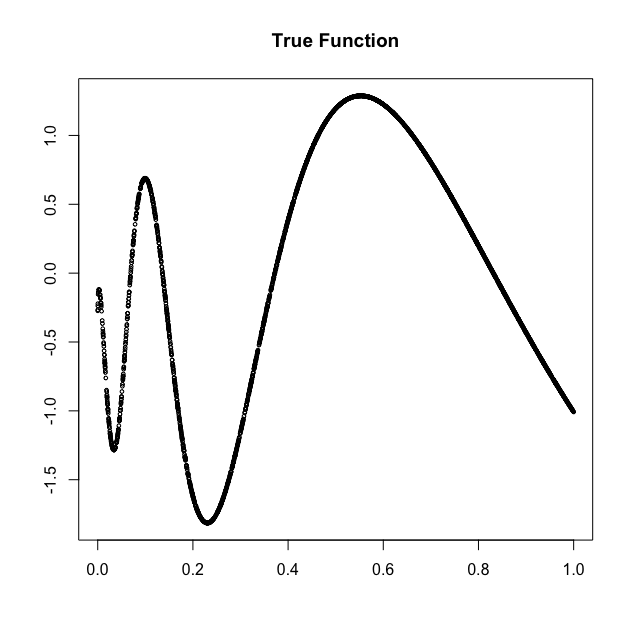
\includegraphics[width=\linewidth,height=2in]{figures/plots/truef.png} % Adjusted width and height of the image
        \caption{True function}
        \label{fig:a}
    \end{subfigure} 
    \begin{subfigure}[b]{0.24\textwidth} % Adjusted width for each subfigure
        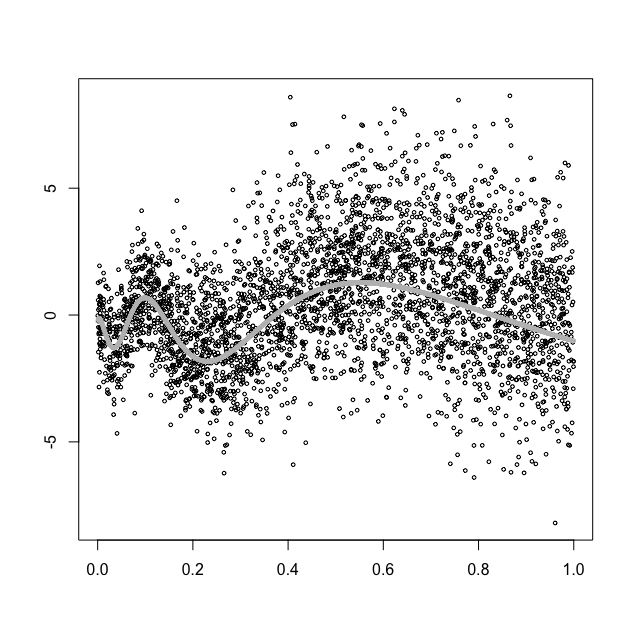
\includegraphics[width=\linewidth,height=2in]{figures/plots/sce1noise.png} % Adjusted width and height of the image
        \caption{Scenario 1 Noise}
        \label{fig:b}
    \end{subfigure}       
    \begin{subfigure}[b]{0.24\textwidth} % Adjusted width for each subfigure
        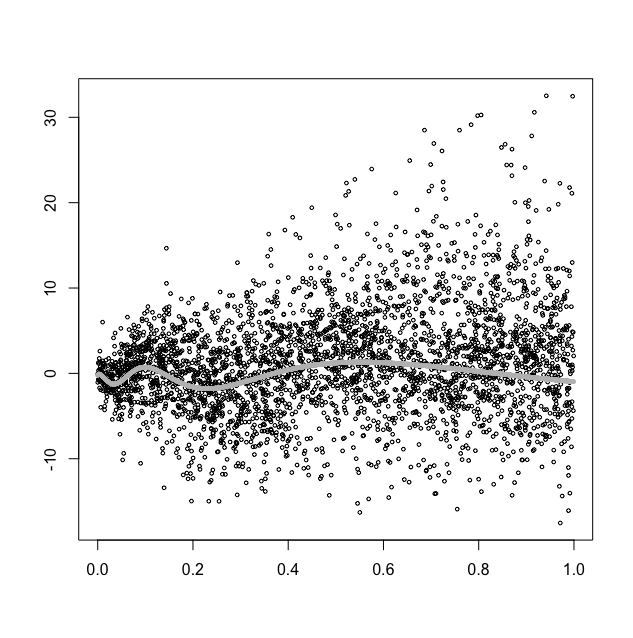
\includegraphics[width=\linewidth,height=2in]{figures/plots/sce2noise.png} % Adjusted width and height of the image
        \caption{Scenario 2 Noise}
        \label{fig:c}
    \end{subfigure}     
    \begin{subfigure}[b]{0.24\textwidth} % Adjusted width for each subfigure
        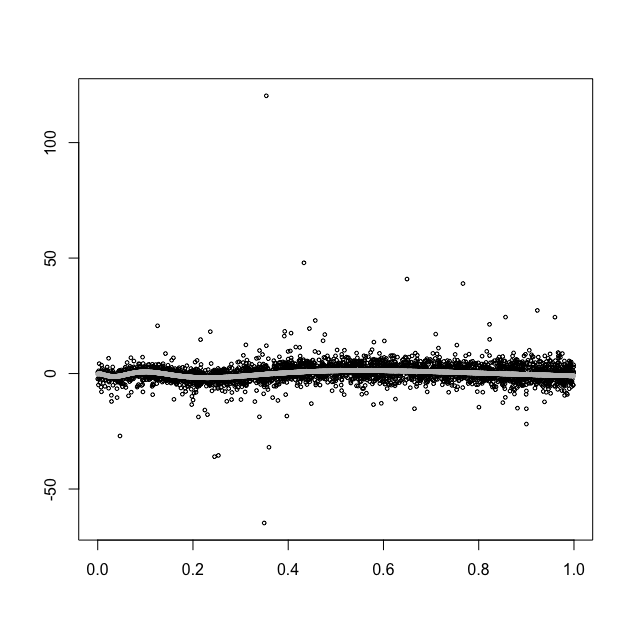
\includegraphics[width=\linewidth,height=2in]{figures/plots/sce3noise.png} % Adjusted width and height of the image
        \caption{Scenario 3 Noise}
        \label{fig:d}
    \end{subfigure} 
    % \vspace{-1em}
    \caption[]{Panel \subref{fig:a} is the true function $f^*$. Panels \subref{fig:b}, \subref{fig:c}, and \subref{fig:d}} are example plots of the noisy data with $n=200$ and $m\_mult=1$. 
    \label{fig:all env}
\end{figure*}

\begin{figure*}[htb]
    \captionsetup[subfigure]{aboveskip=-1pt,belowskip=-1pt,font=footnotesize}
    \centering
    \begin{subfigure}[b]{0.3\textwidth} % Adjusted width for each subfigure
        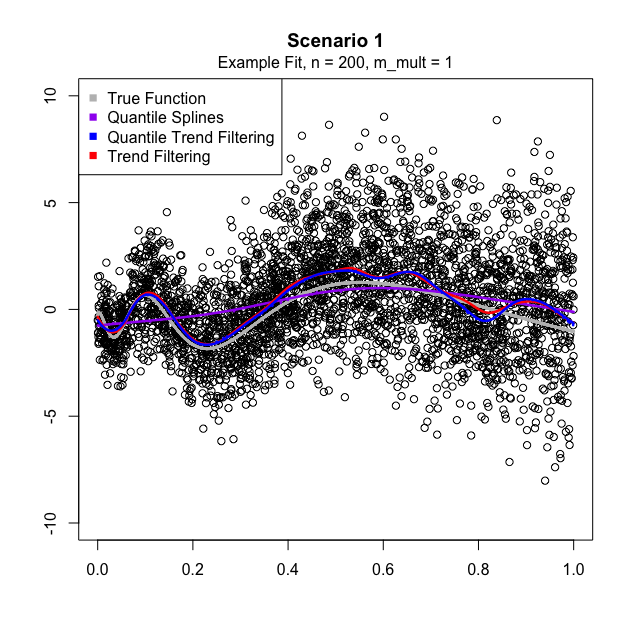
\includegraphics[width=\linewidth,height=2in]{figures/plots/sce1ex.png} % Adjusted width and height of the image
        \caption{Scenario 1 Example Fit}
        \label{fig:a}
    \end{subfigure}       
    \begin{subfigure}[b]{0.3\textwidth} % Adjusted width for each subfigure
        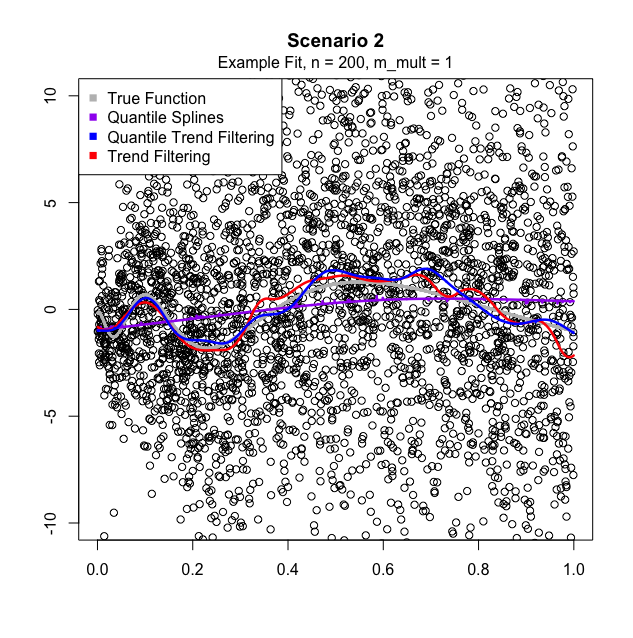
\includegraphics[width=\linewidth,height=2in]{figures/plots/sce2ex.png} % Adjusted width and height of the image
        \caption{Scenario 2 Example Fit}
        \label{fig:b}
    \end{subfigure}     
    \begin{subfigure}[b]{0.3\textwidth} % Adjusted width for each subfigure
        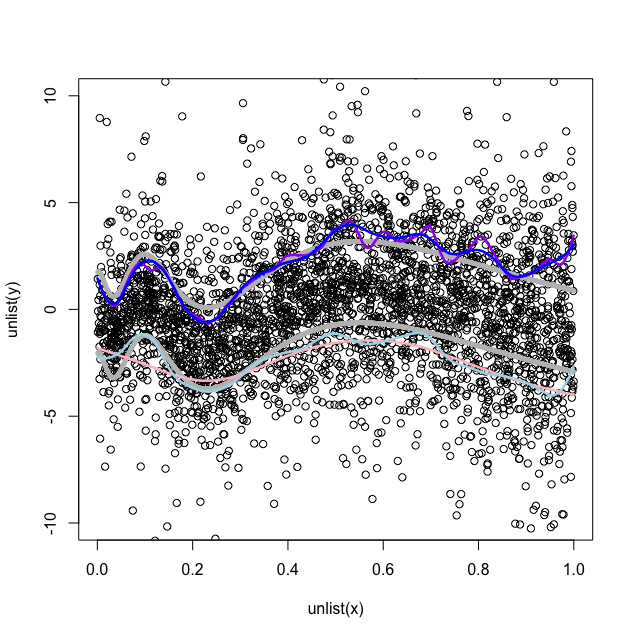
\includegraphics[width=\linewidth,height=2in]{figures/plots/sce3ex.png} % Adjusted width and height of the image
        \caption{Scenario 3 Example Fit}
        \label{fig:c}
    \end{subfigure} 
    % \vspace{-1em}
    \caption[]{Panels \subref{fig:a}, \subref{fig:b}, and \rev{\subref{fig:c}}} are examples of the fitted curves of TF, QTF, and QSS with $n=200$ and $m\_mult=1$. 
    \label{fig:all env}
\end{figure*}


\subsection{Multivariate Study}
For all the following scenarios, we consider \( f^* = f - \int_{0}^{1} f(x)dx \) for the following piecewise constant function:
\[
f_0(x) =
\begin{cases} 
1 & \text{if } \|x - \frac{1}{4} \mathbf{1}_d\|_2 < \| x - \frac{3}{4} \mathbf{1}_d \|_2, \\
-1 & \text{otherwise},
\end{cases}
\]

\begin{enumerate}
    
\item \textbf{Scenario 1}: We take $G_i\sim N(0, 1)$, $F_i\sim N(0, 0.5)$, and $d=2$. This scenario may serve as a baseline. 

\item \textbf{Scenario 2}: We take $G_i\sim t(2)$, $F_i\sim \text{cauchy}(0, 1)$, and $d=2$. $t(2)$ denotes the t-distribution with 2 degrees of freedom. 

\item \textbf{Scenario 3}: We take $G_i\sim N(0, 1)$, $F_i\sim N(0, 1)$, and consider $\tau = 0.2$ and $\tau = 0.8$ $d=2$. 

% However, we also scale the measurement errors $\tilde e_{ij}$ by $\|x_{ij}\|_2$, so the quantiles of the measurement errors correlate with the inputs. We consider $\tau = 0.2$ and $\tau = 0.8$, with the necessary predicted values for the coverage calculation acquired using 1-NN interpolation. 

\item \textbf{Scenario 4}: We take $G_i\sim N(0, 2)$, and $F_i\sim t(3)$. However, here we consider $d = 5$ and $d = 10$. 

\end{enumerate}


\subsection{Non-Convex Study}

We further study a non-convex setting by replacing the convex estimators in the multivariate study with neural networks. 
We consider two neural-network baselines with identical architectures, differing only in the training loss:
(i) a squared-error network (SqErr Network) trained by minimizing the mean squared error loss, and 
(ii) a quantile network (Quantile Network) trained by minimizing the pinball loss for a set of target quantile levels 
$\mathcal{Q}=\{0.1,0.3,0.5,0.7,0.9\}$.


We consider three spatial-temporal scenarios (Scenarios~6--8) in the multivariate setting with $d=2$.
All three scenarios follow the common sampling scheme described in Section~\ref{subsec:simulated_data} (Simulated data), 
including the heterogeneous per-time sample sizes $\{m_i\}_{i=1}^n$, the temporally dependent design points $\{x_{ij}\}$, 
and the spatio-temporal noise components $\delta_i(\cdot)$ and $e_i$.
Specifically, for each $i\in[n]$ and $j\in[m_i]$, the response is generated as
\begin{equation}\label{eq:st_yij}
y_{ij} \;=\; \beta(x_{ij}) \;+\; \delta_i(x_{ij}) \;+\; e_{ij},
\end{equation}
where the signal $\beta(\cdot)$ is the piecewise-constant function
\begin{equation}\label{eq:st_beta_piecewise}
\beta(x)=
\begin{cases}
1, & \text{if } \left\|x-\frac14\mathbf{1}_d\right\|_2 < \left\|x-\frac34\mathbf{1}_d\right\|_2,\\
-1, & \text{otherwise}.
\end{cases}
\end{equation}

\smallskip
\noindent\textbf{Design points and flattening.}
For a fixed temporal length $n$, we first generate a padded array $\{x_{i\ell}\}_{\ell=1}^M$ with $M=\max_i m_i$ by sampling 
$x_{1\ell}\stackrel{\text{i.i.d.}}{\sim}\mathrm{Unif}([0,1]^d)$ and then, for $i\,\ge\, 2$, copying each previous location with probability $\phi=0.1$ 
(as in \eqref{eq:st_xij} in Section~\ref{subsec:simulated_data}); we only keep the first $m_i$ locations at time $i$, i.e., $\{x_{ij}\}_{j=1}^{m_i}$.
The training set used by neural networks is obtained by flattening the panel data
$\{(x_{ij},y_{ij})\}_{i=1,j=1}^{n,m_i}$ into \rev{flattened input--response pairs}:
\[
X_{\mathrm{train}}=\big[x_{11};\ldots;x_{1m_1};x_{21};\ldots;x_{nm_n}\big]\in\mathbb{R}^{(\sum_i m_i)\times d}, 
\qquad 
y_{\mathrm{train}}=\big[y_{11},\ldots,y_{nm_n}\big]^\top\in\mathbb{R}^{\sum_i m_i}.
\]
The test set is formed in the same way using an independently generated panel of design points.

\smallskip
\noindent\textbf{Spatial noise.}
The spatio-temporal component $\delta_i(\cdot)$ follows the recursive construction in \eqref{eq:st_delta_def}:
\begin{equation}\label{eq:st_delta_nn}
\delta_i(x)\;=\;0.5\,\delta_{i-1}(x)\;+\;\sum_{t=1}^{25} t^{-1} b_{i,t}\, h_t(x),
\qquad b_{i,t}\sim G_i,
\end{equation}
where $\{h_t\}_{t=1}^{25}$ are sine-basis functions as in~\eqref{eq:h_t_def}. 
In implementation, for each location $x=(x(1),\ldots,x(d))\in[0,1]^d$, we use
\begin{equation}\label{eq:st_ht}
h_t(x)\;=\;\prod_{r=1}^d \left(\frac{\pi}{\sqrt{2}}\sin\big(t\,x(r)\big)\right),\qquad t=1,\ldots,25.
\end{equation}

\smallskip
\noindent\textbf{Measurement error.}
The measurement error is generated via the AR-type recursion in \eqref{eq:st_e_def}:
\begin{equation}\label{eq:st_e_nn}
\tilde e_i \;=\; 0.3\,\tilde e_{i-1} \;+\; \xi_i,\qquad \xi_i\sim F_i,
\end{equation}
where $\tilde e_i\in\mathbb{R}^M$, and we set $e_{ij}$ to be the $j$th entry of $\tilde e_i$ for $j\,\le\, m_i$.

\smallskip
\noindent\textbf{Scenario specifications.}
The scenarios differ only through the innovation distributions $G_i$ and $F_i$ and the quantile level $\tau$:
\begin{itemize}
    \item \textbf{Scenario 6 (light-tailed):} $b_{i,t}\stackrel{\text{i.i.d.}}{\sim}N(0,1)$ and $\xi_i(\ell)\stackrel{\text{i.i.d.}}{\sim}N(0,0.5^2)$.
    \item \textbf{Scenario 7 (heavy-tailed):} $b_{i,t}\stackrel{\text{i.i.d.}}{\sim}t(5)$ and $\xi_i(\ell)\stackrel{\text{i.i.d.}}{\sim}t(5)$, leading to heavier tails in both $\delta_i(\cdot)$ and $e_i$.
    \item \textbf{Scenario 8 
    % ($\tau\neq 0.5$ with variance-stabilized recursion)
    :}
we consider $\tau=0.5$ and define the target quantile signal as 
$\beta_\tau(x)=f_0(x)+\Phi^{-1}(\tau)$.
The spatial-noise coefficients follow an AR-type recursion:
for $t=1,\ldots,25$, let $z_{i,t}\stackrel{\mathrm{i.i.d.}}{\sim}N(0,1)$ and set
\[
b_{i,t}=\frac{0.5\,b_{i-1,t}+t^{-1}z_{i,t}}{s_\delta},
\qquad s_\delta=\sqrt{0.5^2+1^2},
\]
(with $s_\delta=1$ at $i=1$), and define $\delta_i(x)=\sum_{t=1}^{25} b_{i,t}h_t(x)$.
The measurement error is generated by
$u_{i,\ell}\stackrel{\mathrm{i.i.d.}}{\sim}t(3)$ and
\[
\tilde e_i(\ell)=\frac{0.3\,\tilde e_{i-1}(\ell)+u_{i,\ell}}{s_e},
\qquad s_e=\sqrt{0.3^2+1^2},
\]
(with $s_e=1$ at $i=1$), and we take $e_{ij}=\tilde e_i(j)$ for $j\,\le\, m_i$.
Finally, $y_{ij}=\beta_\tau(x_{ij})+\delta_i(x_{ij})+e_{ij}$.
\end{itemize}

% \paragraph{Data generating scenarios.}
% We focus on three spatial-temporal scenarios (Scenarios 6--8) with $d=2$ and temporal dependence in both the spatial noise and measurement error.
% The true signal is the piecewise-constant function 
% \[
% f_0(x)=
% \begin{cases} 
% 1 & \text{if } \|x - \frac{1}{4}\mathbf{1}_d\|_2 < \|x - \frac{3}{4}\mathbf{1}_d\|_2,\\
% -1 & \text{otherwise}.
% \end{cases}
% \]
% The spatial noise is generated by a sine-basis expansion with temporal dependence, and the measurement error follows an AR-type recursion.
% Scenario 6 uses Gaussian innovations (light-tailed), Scenario 7 uses heavy-tailed innovations, and Scenario 8 considers $\tau\neq 0.5$ with a normalization to keep the variance stable across time indices.

\paragraph{Evaluation metric.}
For each quantile level $q\in\mathcal{Q}$, we evaluate the squared error between the learned quantile function and the oracle quantile function on a large test set, and report the average over Monte Carlo trials.
We vary the temporal length $n\in\{100,500,1000\}$ (with the corresponding $\{m_i\}$ pattern described above).

\paragraph{Summary of findings.}
Table~\ref{tab:nn_nonconvex} shows that the Quantile Network consistently outperforms the SqErr Network across all three scenarios and all quantile levels.
The improvements are particularly pronounced for tail quantiles ($q=0.1$ and $q=0.9$), where minimizing squared error is misaligned with the quantile target and heavy-tailed errors exacerbate the discrepancy.
In contrast, the pinball loss directly targets the conditional quantiles and yields substantially smaller errors, especially in Scenarios 6 and 8.


\begin{table*}[t]
\centering
\caption{Non-convex study: test-set MSE between predicted and oracle quantile functions for five quantile levels
$\mathcal{Q}=\{0.1,0.3,0.5,0.7,0.9\}$.
We compare a squared-error network (SqErr) and a quantile network (Quantile). The best performance is \textbf{bolded}.}
\label{tab:nn_nonconvex}
\small
\setlength{\tabcolsep}{5pt}
\renewcommand{\arraystretch}{1.15}
\begin{tabular}{llccccc}
\toprule
Scenario & Method ($n$) & $q=0.1$ & $q=0.3$ & $q=0.5$ & $q=0.7$ & $q=0.9$ \\
\midrule
\multirow{6}{*}{Scenario 6}
& SqErr (100)  & 21.717 & 6.522 & 3.060 & 5.422 & 19.034 \\
& Quantile (100) & \textbf{3.702} & \textbf{2.486} & \textbf{2.457} & \textbf{3.097} & \textbf{7.141} \\
& SqErr (500)  & 23.058 & 7.071 & 3.059 & 4.870 & 17.690 \\
& Quantile (500) & \textbf{2.625} & \textbf{2.243} & \textbf{2.205} & \textbf{2.333} & \textbf{2.799} \\
& SqErr (1000) & 23.409 & 7.220 & 3.067 & 4.737 & 17.355 \\
& Quantile (1000) & \textbf{2.516} & \textbf{2.251} & \textbf{2.150} & \textbf{2.136} & \textbf{2.308} \\
\midrule
\multirow{6}{*}{Scenario 7}
& SqErr (100)  & 37.480 & 9.810 & 4.067 & 7.505 & 30.190 \\
& Quantile (100) & \textbf{4.913} & \textbf{3.982} & \textbf{4.513} & \textbf{5.058} & \textbf{7.696} \\
& SqErr (500)  & 37.040 & 9.618 & 4.031 & 7.630 & 30.553 \\
& Quantile (500) & \textbf{3.864} & \textbf{3.730} & \textbf{3.810} & \textbf{4.186} & \textbf{5.119} \\
& SqErr (1000) & 32.095 & 7.612 & 3.893 & 9.374 & 35.126 \\
& Quantile (1000) & \textbf{4.742} & \textbf{3.965} & \textbf{3.687} & \textbf{3.792} & \textbf{4.796} \\
\midrule
\multirow{6}{*}{Scenario 8}
& SqErr (100)  & 19.419 & 5.226 & 2.750 & 7.078 & 26.661 \\
& Quantile (100) & \textbf{2.409} & \textbf{2.079} & \textbf{1.854} & \textbf{1.883} & \textbf{2.237} \\
& SqErr (500)  & 22.925 & 6.557 & 2.557 & 5.264 & 22.440 \\
& Quantile (500) & \textbf{1.803} & \textbf{1.631} & \textbf{1.644} & \textbf{1.667} & \textbf{1.805} \\
& SqErr (1000) & 22.870 & 6.533 & 2.556 & 5.287 & 22.498 \\
& Quantile (1000) & \textbf{2.018} & \textbf{1.671} & \textbf{1.643} & \textbf{1.637} & \textbf{1.696} \\
\bottomrule
\end{tabular}
\end{table*}




% \blindmathpaper

% Here is a citation \cite{chow:68}.

% Acknowledgements and Disclosure of Funding should go at the end, before appendices and references

\acks{All acknowledgements go at the end of the paper before appendices and references.
Moreover, you are required to declare funding (financial activities supporting the
submitted work) and competing interests (related financial activities outside the submitted work).
More information about this disclosure can be found on the JMLR website.}

% Manual newpage inserted to improve layout of sample file - not
% needed in general before appendices/bibliography.

\newpage

\appendix
% \input{a1_quantile_temporal_spatial_appendix_v14}
\section{Proof of Theorem~\ref{Theorem_1}}
\label{app_b}

\subsection{Definitions and Notation}
To complete our proofs for the theorems, we provide important definitions.
% Let $J$ as in Definition~\ref{definition2}. 
% \begin{definition} 
% The $r$-th order $TV$-ball of radius $V$ is defined as: 
% \label{def:J}
% \beq 
% \label{eq197}
% B_J(V) \coloneqq B_{TV}^{(r)}(V) = \set{f: TV^{(r)}(f) = J(f) \le V}. 
% % \equiv\ \set{f: J(f)\le V}
% \beq
% \end{definition}
% \begin{definition}
% The $r$-th order trend filtering operator norm ball of radius $V$ as 
% \beq 
% \label{def:ball of trend filtering}
% BV^{(r)}(V) = \set{\theta \in \R^n: \norm{D^{(x,r)}(\theta)}_1 \le V}.
% \beq    
% \end{definition}

% Let $y\in \R^n$ be a vector of independent random variables and for a given quantile level $\tau \in (0,1)$.    

\begin{definition}
We introduce the Huber-type \cite{huber1992robust} loss. 
Let $\Delta_{nm}^2$ be a mapping of functions to real numbers,
the Huber-type loss function is elucidated as
% \beq 
% \label{huber loss}
% \Delta^2(f, \{x_{ij}\}) = \frac{1}{n} \sum_{i=1}^n \frac{1}{m_i} \sum_{j=1}^{m_i} \min\{\abs{f(x_{ij})}, (f(x_{ij}))^2\},
% \beq 
\beq 
\label{huber loss}
\Delta_{nm}^2(f) \,=\, \frac{1}{n} \sum_{i=1}^n \frac{1}{m_i} \sum_{j=1}^{m_i} \min\{\abs{f(x_{ij})}, (f(x_{ij}))^2\},
\beq 
which, modulo constants, corresponds to a Huber loss, as delineated in \cite{huber1992robust}. The Huber loss serves as a natural lower bound for the quantile population loss, which provides the primary motivation for focusing on it.
\begin{revision}
Let $Q$ denote the design distribution on $[0,1]^d$. The population Huber loss is
\begin{align}
\label{huber_def}
\Delta^2(f) &\,=\, \int_{[0,1]^d}\min\{\abs{f(t)}, \abs{f(t)}^2\}\,dQ(t).
\end{align}
\end{revision}
We derive the rate of convergence by using the Huber-type  loss and $L_2$ loss. 
\end{definition}



% \begin{definition}
% \label{definition213}
% We define the Rademacher width of $K$ as
% \bea 
% R_{nj}(F_k(V),\{x_{ij}\}) = \ept{\sup_{f \in \gF_k(V)}  \frac{1}{n}\sum_{i=1}^n \xi_{ij} f(x_{ij})\mid \{x_{ij}\}_{i=1}^{n}}.
% \bea    
% \end{definition}


% \begin{definition}
% \label{definition213}
% We define its Empirical Rademacher width as 
% \bea 
% R_{mn}(K) = \ept{\sup_{f \in K}  \frac{1}{n}\sum_{i=1}^n \frac{1}{m_i}\sum_{j=1}^{m_{i}} \xi_{ij} f(x_{ij})\mid \{x_{ij}\}_{i=1,j=1}^{n,m_{ij}}}.
% \bea    
% \end{definition}


% \begin{definition}
% \label{def_rade}
%  we define its Rademacher width 
% \bea 
% R(K) = \ept{R_{mn}(K)} = \ept{\sup_{f \in K}  \frac{1}{n}\sum_{i=1}^n \frac{1}{m_i}\sum_{j=1}^{m_{i}} \xi_{ij} f(x_{ij})}. 
% \bea
% \end{definition}


\begin{definition}
\label{definition213} Let $K$ be a function class with Rademacher width well defined. 
We define its Empirical Rademacher width as 
\bea 
R_{mn}(K) \,=\, \Ept{\xi \mid \{x_{ij}\}}{\sup_{f \in K}  \frac{1}{\sum_{i=1}^n m_i}\sum_{i=1}^n \sum_{j=1}^{m_{i}} \xi_{ij} f(x_{ij})}.
\bea    
\end{definition}


\begin{definition}
\label{def_brade}
 We define its Rademacher width as
\bea 
 R(K) \,=\, \Ept{x}{\Ept{\xi \mid \{x_{ij}\}}{\sup_{f \in K}  \frac{1}{\sum_{i=1}^n m_i}\sum_{i=1}^n \sum_{j=1}^{m_{i}} \xi_{ij} f(x_{ij})}} = \Ept{x, \xi}{\sup_{f \in K}  \frac{1}{\sum_{i=1}^n m_i}\sum_{i=1}^n \sum_{j=1}^{m_{i}} \xi_{ij} f(x_{ij})}. 
\bea
\end{definition}





\begin{definition}
  We define $\hat Z_{ij}(f)$ and  the empirical loss function $\hat Z(f)$ as 
\beq 
\label{348}
\hat Z_{ij}(f) =& \rho_{\tau}(y_{ij}  - f(x_{ij})) - \rho_{\tau}(y_{ij}  - f^*(x_{ij})) \\
=& \rho_{\tau}(f^*(x_{ij}) + \delta_i(x_{ij}) + e_{ij}  - f(x_{ij})) - \rho_{\tau}(\delta_i(x_{ij}) + e_{ij}). 
\beq 
\beq 
\label{295}
\hat Z(f) &\,=\, \frac{1}{n}\sum_{i=1}^n \frac{1}{m_i}\sum_{j=1}^{m_{i}} \hat Z_{ij}(f)\\
&\,=\, \frac{1}{n}\sum_{i=1}^n \frac{1}{m_i}\sum_{j=1}^{m_{i}}\set{ \rho_{\tau}(y_{ij}  - f(x_{ij})) - \rho_{\tau}(y_{ij}  - f^*(x_{ij}))}\\
&\,=\, \rev{\frac{1}{n}\sum_{i=1}^n \frac{1}{m_i}\sum_{j=1}^{m_{i}}\set{\rho_{\tau}(f^*(x_{ij}) + \delta_i(x_{ij}) + e_{ij} - f(x_{ij})) - \rho_{\tau}(\delta_i(x_{ij}) + e_{ij})}}.   
\beq 


We also define $ Z_{ij}(f)$ and $Z(f)$ as 
\beq 
\label{eq215}
Z_{ij}(f) \,\coloneqq\, & \Ept{\delta, e \mid x_{ij}}{\rho_{\tau}(y_{ij}  - f(x_{ij})) - \rho_{\tau}(y_{ij}  - f^*(x_{ij}))} \\
=& \Ept{\delta, e \mid x_{ij}}{\rho_{\tau}(f^*(x_{ij}) + \delta_i(x_{ij}) + e_{ij}  - f(x_{ij})) - \rho_{\tau}(\delta_i(x_{ij}) + e_{ij})}. 
\beq 

% \beq 
% \label{def_zf}
% Z(f) & \coloneqq  \ept{\hat Z(f)|\{x_{ij}\}_{i=1,j=1}^{n,m_{ij}}} \\
% &= \frac{1}{n}\sum_{i=1}^n \frac{1}{m_i}\sum_{j=1}^{m_{i}} \ept{\rho_{\tau}(y_{ij}  - f(x_{ij})) - \rho_{\tau}(y_{ij}  - f^*(x_{ij}))|\{x_{ij}\}_{i=1,j=1}^{n,m_{ij}}} \\
% &=  \frac{1}{n}\sum_{i=1}^n \frac{1}{m_i}\sum_{j=1}^{m_{i}}\ept{\rho_{\tau}(f^*_{ij} + \delta_i(x_{ij}) + e_{ij}  - f(x_{ij})) - \rho_{\tau}(y_{ij}  - f^*(x_{ij}))|\{x_{ij}\}_{i=1,j=1}^{n,m_{ij}} }, 
% \beq 
% where we use $\{x_{ij}\}$ as a shorthand for $\{x_{ij}\}_{i \in \mathcal{J}_{e,l},\; j \in [m_i]}$.

\beq 
\label{def_zf}
Z(f) & \,\coloneqq\,  \Ept{\delta, e \mid \{x_{ij}\}}{\hat Z(f)} \\
&\,=\, \frac{1}{n}\sum_{i=1}^n \frac{1}{m_i}\sum_{j=1}^{m_{i}} \Ept{\delta, e \mid \{x_{ij}\}}{\rho_{\tau}(y_{ij}  - f(x_{ij})) - \rho_{\tau}(y_{ij}  - f^*(x_{ij}))} \\
&\,=\, \rev{\frac{1}{n}\sum_{i=1}^n \frac{1}{m_i}\sum_{j=1}^{m_{i}}\Ept{\delta, e \mid \{x_{ij}\}}{\rho_{\tau}(f^*(x_{ij}) + \delta_i(x_{ij}) + e_{ij} - f(x_{ij})) - \rho_{\tau}(\delta_i(x_{ij}) + e_{ij})}}, 
\beq 

where we use $\{x_{ij}\}$ as a shorthand for $\{x_{ij}\}_{i=1,j=1}^{n,m_{ij}}$ and $\set{\delta_i}$ as $\set{\delta_i}_{i=1}^n$.


We then define $\tilde Z_{ij}(f)$ and $\tilde Z(f)$ as 
\bea 
\tilde Z_{ij}(f) \,\coloneqq\,  \Ept{e \mid \delta_i, x_{ij}}{ \hat Z_{ij}(f)}.
\bea 
\beq 
\label{def_tilde_zf}
\tilde Z(f) \,\coloneqq\,  \Ept{e \mid \set{\delta_i},\set{x_{ij}}}{\hat Z(f)}.
\beq 



We define the population version $\bar Z_{ij}(f)$ and the population loss function as
\bea 
\bar Z_{ij}(f) \,\coloneqq\,  \Ept{x, \delta, e}{ \hat Z_{ij}(f)}.
\bea 
\beq 
\label{305}
\bar Z(f) \,\coloneqq\,  \Ept{x, \delta, e}{\hat Z(f)}. 
\beq  
\end{definition}
 


Note that the $\delta_i(x_{i1}), \dots, \delta_i(x_{im_i})$ are not independent for $i \in \set{1,\dots, n}$. 
Similarly, due to the definitions of $\hat Z_{ij}(f)$, $Z_{ij}(f)$, $\hat Z(f)$, and $Z(f)$, the terms $\hat Z_{i1}(f), \dots, \hat Z_{im_i}(f)$ are also not independent. \rev{Because $Z$ is an excess-risk functional relative to $f^*$, $Z(f^*)=0$ and $Z(f)\geq0$.}
% and $f^*(x_{ij}) = Q_{\tau}(y_i | x_i)$. from \eqref{eq44},


\begin{definition}
\label{definition3}
The constrained quantile trend filtering estimator for temporal-spatial data defined in \eqref{eq172} will be
\label{def}
    \beq 
\hat f = \argmin_{f \in F_k(V)} \hat Z(f),
\beq  where $F_k(V)$ is defined in \eqref{def_tvspace_tf}. 
\end{definition}


\subsection{Proof Sketches of Theorem~\ref{Theorem_1}}

% To proceed in the proof of Theorems~\ref{Theorem_1}, 
\step{Step 1}
To get the convergence rate of $\Delta^2(\hat f - f^*)$, we will control the quantity $\sP\left( c_0\Delta^2(\hat f - f^*) > t^2  \right)$, where $c_0$ satisfies \eqref{eq_c0_range}. 

We will first consider the temporal dependence. To control 
that, we would need to use the $\beta-$mixing concept that are constructed in Appendix~\ref{beta_mix_intro}.
We then get the setup of the indices for \( |\mathcal{J}_{e,l}|, |\mathcal{J}_{o,l}| \asymp n/L \) in \eqref{odd_even_indices}. We let $\gI \,\coloneqq\, \bigcup_{l=1}^{L}(\mathcal J_{e,l}\cup \mathcal J_{o,l})$. \rev{For each fixed $l \in [L]$, we apply the coupling in Appendix~\ref{beta_mix_intro} to the joint clusters $W_i=(X_i,\delta_i,E_i)$ for $i\in\mathcal J_{e,l}$ (and similarly for $\mathcal J_{o,l}$). This constructs coupled clusters
\[
W_i^* \,=\, (X_i^*,\delta_i^*,E_i^*),
\qquad
X_i^* \,=\, (x_{i1}^*,\dots,x_{im_i}^*),
\qquad
E_i^* \,=\, (e_{i1}^*,\dots,e_{im_i}^*),
\]
such that $W_i^*$ has the same joint distribution as $W_i$ and the coupled clusters are mutually independent over $i$ within each fixed block.} We then define
\beq 
\label{omega_definition}
&\Omega_x \,:=\, \left\{ X_i = X_i^* \ \text{for all } i\in \gI \right\},\\
&\Omega_e \,:=\, \left\{ E_i = E_i^* \ \text{for all } i\in \gI \right\}, \\
&\Omega_\delta \,:=\, \left\{ \delta_i = \delta_i^* \ \text{for all } i\in \gI \right\}, \\
&\Omega_\beta \,:=\, \Omega_x\cap \Omega_e\cap \Omega_\delta. 
\beq 

% $\Omega_x := \left\{ X_i = X_i^* \ \text{for all } i\in \gI \right\},$
% $\Omega_e := \left\{ E_i = E_i^* \ \text{for all } i\in \gI \right\}, \\ $
% $\Omega_\delta := \left\{ \delta_i = \delta_i^* \ \text{for all } i\in \gI \right\},$ and 
% $\Omega_\beta := \Omega_x\cap \Omega_e\cap \Omega_\delta .$ 
% \(\Omega_{x} = \{i: x_{ij} = x_{ij}^{*} \ \forall j \in [m_i]\}\), \(\Omega_{e} = \{i: e_{ij} = e_{ij}^{*} \ \forall j \in [m_i]\}\) and \(\Omega_{\delta} = \{i: \delta_{i} = \delta_{i}^{*}, \forall j \in [m_i]\}\), let \(\Omega_{\beta} = \Omega_{x} \cap \Omega_{e} \cap \Omega_{\delta} \).
Thus, we get 
\bea  
\sP\left( c_0\Delta^2(\hat f - f^*) > t^2 \right) \,\leq\, \sP\left(\left\{ c_0\Delta^2(\hat f - f^*) > t^2\right\} \cap \Omega_{\beta}  \right) + \sP\left(\left\{ c_0\Delta^2(\hat f - f^*) > t^2\right\} \cap \Omega_{\beta}^{c}\right). 
\bea 

\step{Step 2}
Then in Lemma~\ref{lemma_beta_decomp}, we show $\sP\left(\left\{ c_0\Delta^2(\hat f - f^*) > t^2\right\} \cap \Omega_{\beta}^{c}\right)$ is $O(\frac{1}{n})$.


\step{Step 3} 
It remains to bound the joint probability
$\sP\!\left(\{c_0\Delta^2(\hat f-f^*)>t^2\}\cap \Omega_\beta\right)$.
On the coupling event $\Omega_\beta$ (see Remark~\ref{remark:joint}),
the blockwise coupling reduces the original $\beta$-mixing sequence to an
independent-block structure. Consequently, the arguments in
Lemmas~\ref{lemma12}--\ref{lem_huber_rate} (based on symmetrization and
Rademacher complexities) yield an upper bound for
$\sP\!\left(\{c_0\Delta^2(\hat f-f^*)>t^2\}\cap \Omega_\beta\right)$
in terms of the corresponding blockwise Rademacher width terms. 
% The details of the proof are provided as follows. 
% We first define empirical loss function $\hat Z(f)$ as in \eqref{295}, 
% \bea 
% \hat Z(f) &= \frac{1}{n}\sum_{i=1}^n \frac{1}{m_i}\sum_{j=1}^{m_{i}} \hat Z_{ij}(f)\\
% &= \frac{1}{n}\sum_{i=1}^n \frac{1}{m_i}\sum_{j=1}^{m_{i}}\set{ \rho_{\tau}(y_{ij}  - f(x_{ij})) - \rho_{\tau}(y_{ij}  - f^*(x_{ij}))}.
% \bea and its conditional expectation parts as 
% \bea 
% Z(f) =  \ept{\hat Z(f)|\set{x_{ij}}}, \quad \tilde Z(f) \coloneqq  \ept{\hat Z(f)|\set{\delta_i},\set{x_{ij}}}, \quad \bar Z(f) \coloneqq  \ept{\hat Z(f)}. 
% \bea 
\step{Step 4}
\begin{revision}
Under the hypotheses of Lemma~\ref{lem_huber_rate}, use the auxiliary
response groups $\mathcal A_r$ in
Lemma~\ref{lem_nonconvex_auxiliary_groups}. Direct aggregation with
the original empirical weights gives, for every $t>0$,
\bea
\mathbb P\{c_0\Delta^2(\hat f-f^*)>t^2\}
&\le\frac1n+\frac{9C}{cLt^2}
 \sum_{r=1}^L R_{\mathcal A_r}
 \left(\{f-f^*:f\in\mathcal F,\ c_0\Delta^2(f-f^*)\le t^2\}\right)\\
&\quad+\frac{4\max\{1,2B\}L}{(C_0-c_0)nt^2}.
\bea
The term $1/n$ bounds the failure probability of the common response
coupling. The remaining terms follow by summing the three conditional
loss components and allocating $\ell(f)/L$ to each auxiliary group.
\end{revision}


\step{Step 5}
\begin{revision}
Under the hypotheses of Lemma~\ref{lem_huber_rate}, use
Lemma~\ref{lem_l2} to convert the Huber-localized widths to
$L_2(Q)$-localized widths in each auxiliary group. Choose a
deterministic sequence $r_n>0$ satisfying
\eqref{eq_op_sufficient_radius} for some constant $A$ independent
of $n$. Corollary~\ref{cor_op} then gives
\[
\Delta^2(\hat f-f^*)\,=\,O_P(r_n^2).
\]
Lemma~\ref{lem_17} converts this to
$\|\hat f-f^*\|_2^2=O_P(b^2(B)r_n^2)$.
\end{revision}

The details of the proofs of the above steps are provided as follows. 

\subsection{Technical Results for Proofs of Theorem~\ref{Theorem_1}}

\subsection{Proof of Step 1 and 2}
To get the convergence rate of $\Delta^2(\hat f - f^*)$, we will control the quantity $\sP\left( c_0\Delta^2(\hat f - f^*) > t^2  \right)$, where $c_0$ satisfies \eqref{eq_c0_range}, we will first consider the temporal dependence. To control 
that, we would need to use the $\beta-$mixing concept. In the following analysis, we will then deal with this dependence.  

Specifically, we rely on the condition that \( cm \,\leq\, m_i \,\leq\, Cm \) for some positive constants \( c, C \). Additionally, we define
\begin{equation}
\label{equation}
L = \left\lceil \frac{1}{C_{\beta}} 2\log(n) \right\rceil,
\end{equation}
leading us to the conclusion that
\begin{equation}
\label{beta_decay_rate}
\beta_W(L) \,\leq\, \frac{1}{n^{2}},
\end{equation} where $\beta_W$ is defined in Assumption~\ref{ass_c_beta}.
\rev{Throughout our discussion, $W_i^*=(X_i^*,\delta_i^*,E_i^*)$ denotes the coupled cluster constructed in Appendix~\ref{beta_mix_intro}; its coordinates are denoted by $x_{ij}^*$, $\delta_i^*$, and $e_{ij}^*$.} Furthermore, as delineated in Appendix~\ref{beta_mix_intro}, during the formation of these copies the quantities \( |\mathcal{J}_{e,l}| \) and \( |\mathcal{J}_{o,l}| \) in \eqref{odd_even_indices}, which represent the count of even and odd blocks respectively, satisfy \( |\mathcal{J}_{e,l}|, |\mathcal{J}_{o,l}| \asymp n/L \). Thus, there exist positive constants \( c_1 \) and \( c_2 \) such that
 \begin{equation}
 \label{beta_constants}
c_1 n/L \,\leq\, |\mathcal{J}_{e,l}|, |\mathcal{J}_{o,l}| \,\leq\, c_2 n/L, 
\quad L = \left\lceil \frac{1}{C_{\beta}} 2\log(n) \right\rceil.
\end{equation}

\begin{lemma}
\label{lemma_beta_decomp}  
\rev{Let $n\ge2$ and $t>0$.}
Let $\hat f$, $f^*$ belong to $\mathcal{F}$, and let $\Delta^2(\hat f - f^*)$ be the Huber loss. Suppose Assumption~\ref{Assumption 1.} holds with the $\beta$-mixing condition satisfied in \eqref{beta_decay_rate} and the block indices $\mathcal{J}_{e,l}, \mathcal{J}_{o,l}$ satisfying $|\mathcal{J}_{e,l}|, |\mathcal{J}_{o,l}| \asymp n/L$ as in \eqref{odd_even_indices}. \rev{For each fixed $l \in [L]$, construct the coupled clusters $\{W_i^*\}_{i\in\mathcal J_{e,l}}$ that are mutually independent within $\mathcal J_{e,l}$ (and similarly for $\mathcal J_{o,l}$) via Lemma~\ref{Lemma_9}.} Let
$\Omega_{x}, \Omega_{e}, \Omega_{\delta}, \Omega_{\beta}$ be defined in \eqref{omega_definition}. 
% \(\Omega_{x} = \{i: x_{ij} = x_{ij}^{*} \ \forall j \in [m_i]\}\), \(\Omega_{e} = \{i: e_{ij} = e_{ij}^{*} \ \forall j \in [m_i]\}\) and \(\Omega_{\delta} = \{i: \delta_{i} = \delta_{i}^{*}\}\), let \(\Omega_{\beta} = \Omega_{x} \cap \Omega_{e} \cap \Omega_{\delta} \).
Then we have 
\bea  
\sP\left( c_0\Delta^2(\hat f - f^*) > t^2 \right) \,\leq\,  \sP\left(\left\{ c_0\Delta^2(\hat f - f^*) > t^2\right\} \cap \Omega_{\beta} \right)  \,+\, \rev{\frac{1}{n}}.
\bea
\rev{For any $\varepsilon>0$, the remainder is at most $\varepsilon/2$
whenever $n\ge\lceil2/\varepsilon\rceil$, in addition to the stated block conditions.}
\end{lemma}

\begin{proof}
\rev{By Lemma~\ref{Lemma_9} and a union bound over the $n$ time clusters,
\[
\sP(\Omega_\beta^c)
\,\leq\, \sum_{i=1}^n \sP(W_i\neq W_i^*)
\,\leq\, n\beta_W(L)
\,\leq\, \frac{1}{n}.
\]}
Therefore letting
\beq 
\label{event_beta}
\Omega_{\beta} \,=\, \Omega_{x} \cap \Omega_{e} \cap \Omega_{\delta} 
\beq 
we have that
\bea  
\sP\left( c_0\Delta^2(\hat f - f^*) > t^2 \right) &\,=\, \sP\left(\left\{ c_0\Delta^2(\hat f - f^*) > t^2\right\} \cap \Omega_{\beta}  \right) \,+\, \sP\left(\left\{ c_0\Delta^2(\hat f - f^*) > t^2\right\} \cap \Omega_{\beta}^{c}\right) \\
&\,\leq\, \sP\left(\left\{ c_0\Delta^2(\hat f - f^*) > t^2\right\} \cap \Omega_{\beta} \right) \,+\, \frac{1}{n}
% & = \sP\paren{c_0\Delta^2(\hat f - f^*) > t^2|\Omega_\beta} \sP\paren{\Omega_\beta} + \frac{\varepsilon}{2}\\ 
% & \leq \sP\paren{c_0\Delta^2(\hat f - f^*) > t^2|\Omega_\beta}  + \frac{\varepsilon}{2}, 
\bea 
\rev{If $n\ge\lceil2/\varepsilon\rceil$, then $1/n\le\varepsilon/2$,
proving the final assertion.}
\end{proof}
By previous lemma, in consequence, it is enough to bound the term
\beq 
\label{bound_first_term}
\sP\left(\left\{ c_0\Delta^2(\hat f - f^*) > t^2\right\} \cap \Omega_{\beta} \right).
\beq 
% To bound $
% \sP\left(\left\{ c_0\Delta^2(\hat f - f^*) > t^2\right\} \cap \Omega_{\beta} \right)$, it suffices to control  $\sP(\left\{ c_0\Delta^2(\hat f - f^*) > t^2\right\}\mid \Omega_\beta)$.  

To this end, we will work with the indicator of the coupling event.
We write $\indic{\Omega_\beta}$ for the indicator of $\Omega_\beta$.

We write $\sP(\cdot \cap \Omega_\beta)$ for the probability restricted to $\Omega_\beta$. We denote by $\Ept{x, \delta, e}{\cdot}$ the expectation taken over  $(x_{ij}, \delta_i, e_{ij})$. 
And we denote by $\Ept{e \mid x_{ij}}{\cdot}$ the conditional expectation taken over $ \left\{x_{ij} \right\}_{i=1,j=1}^{n,m_i}$ respectively.

In particular, for any nonnegative random variable $X$, we write
\[
\Ept{x, \delta, e, x^*, \delta^*, e^*}{X\,\indic{\Omega_\beta}}
\]
to denote the expectation of $X$ restricted to the coupling event $\Omega_\beta$. 
\begin{remark}
\label{remark:joint}


\rev{Moreover, on $\Omega_\beta$ we work with the coupled sample
$\{(x_{ij}^*,y_{ij}^*)\}_{i \in \mathcal{J}_{e,l},j\in[m_i]}$, whose time clusters are independent within each fixed block $\mathcal{J}_{e,l}$.}
We now define the star versions of the loss quantities.
The star empirical loss is
\beq 
\label{def_hat_z_star}
\hat Z_{ij}^*(f) \,\coloneqq\, \rho_{\tau}(f^*(x_{ij}^*) + \delta_i^*(x_{ij}^*) + e_{ij}^*  - f(x_{ij}^*)) - \rho_{\tau}(\delta_i^*(x_{ij}^*) + e_{ij}^*),
\beq 
and the star conditional expectations are
\bea 
Z_{ij}^*(f) &\,\coloneqq\,  \Ept{\delta^*, e^* \mid x_{ij}^*}{ \hat Z_{ij}^*(f)}, \\
\tilde Z_{ij}^*(f) &\,\coloneqq\,  \Ept{e^* \mid \delta_i^*, x_{ij}^*}{ \hat Z_{ij}^*(f)}, \\
\bar Z_{ij}^*(f) &\,\coloneqq\,  \Ept{x^*, \delta^*, e^*}{ \hat Z_{ij}^*(f)}.
\bea 
\rev{By construction, for each fixed $l \in [L]$, the star quantities $\{\hat Z_{ij}^*(f)\}_{i \in \mathcal{J}_{e,l}, j \in [m_i]}$ are built from the coupled clusters $\{W_i^*\}_{i \in \mathcal{J}_{e,l}}$, and hence the indices $i \in \mathcal{J}_{e,l}$ are independent (similarly for $\mathcal{J}_{o,l}$). Each $W_i^*$ has the same joint distribution as $W_i$; the copies across different blocks $l$ need not be mutually independent.}
On the coupling event $\Omega_\beta$ we have $(x_{ij}, e_{ij}, \delta_i) \,=\, (x_{ij}^*, e_{ij}^*, \delta_i^*)$ for all $i \in \gI$ and $j \in [m_i]$, so that
\beq 
\label{eq:Z_equal_on_Omega}
\hat Z_{ij}(f) \,=\, \hat Z_{ij}^*(f), \quad Z_{ij}(f) \,=\, Z_{ij}^*(f), \quad \tilde Z_{ij}(f) \,=\, \tilde Z_{ij}^*(f), \quad \bar Z_{ij}(f) \,=\, \bar Z_{ij}^*(f), \qquad \text{on } \Omega_\beta.
\beq 
 \end{remark}
Results that do not invoke the coupling argument remain valid under the
original probability measure and will be indicated explicitly when used.

 
% \begin{remark}
% \label{remark:joint}
% The lemmas below are stated and proved under the joint probability space with the event $\Omega_\beta$ defined in~\eqref{event_beta}.
% The probability of $\Omega_\beta^c$ has already been controlled in Lemma~\ref{lemma_beta_decomp}.
% \end{remark}

\subsection{Proof of Step 3}
Lemma~\ref{lemma_basic_inequality} -- Corollary~\ref{extension of lemma13} are some fundamental lemmas support our convergence analysis. 

\begin{lemma}[Basic Inequality]
\label{lemma_basic_inequality}
By Definitions in \eqref{main_est} and \eqref{295}, we have 
\bea 
\hat Z(\hat f) - \hat Z(f ^*) \,\le\, 0
\bea as the basic inequality. 
\end{lemma}

\begin{lemma}[Lipschitz condition of $\hat Z_{ij}(f)$, $Z_{ij}(f)$ and $r_{ij}(f)$]
\label{lem:lip}
The quantities $\hat Z_{ij}(f)$ (defined in \eqref{348}), $Z_{ij}(f)$ (defined in \eqref{eq215}), and $r_{ij}(f)$ (defined in \eqref{def_rij}) are $1$-Lipschitz in the following sense: for any $f, g \in \mathcal{F}$ and all $(i,j)$,
\bea
\abs{\hat Z_{ij}(f) - \hat Z_{ij}(g)} &\,\leq\, \abs{f(x_{ij}) - g(x_{ij})}, \\
\abs{Z_{ij}(f) - Z_{ij}(g)} &\,\leq\, \abs{f(x_{ij}) - g(x_{ij})}, \\
\abs{r_{ij}(f) - r_{ij}(g)} &\,\leq\, \abs{f(x_{ij}) - g(x_{ij})}.
\bea
\end{lemma}
\begin{proof}

For $\hat Z_{ij}(f)$ and $Z_{ij}(f)$, their Lipschitz condition can be seen in the Lemma A.11 of \cite{zhang2023risk}. 
\begin{revision}
For the remainder, fix $(i,j)$ and write
$a=f(x_{ij})-f^*(x_{ij})$ and $b=g(x_{ij})-f^*(x_{ij})$.
Using the same conditional CDF kernels in \eqref{def_rij}, we have
\bea
\abs{r_{ij}(f)-r_{ij}(g)}
&\labelrel = {eq_rij_lip_integral}
\Bigg|\int_b^a\Big\{
\mathbb P(y_{ij}\leq f^*(x_{ij})+u\mid x_{ij})\\
&\qquad-\mathbb P(y_{ij}\leq f^*(x_{ij})+u
                  \mid\delta_i,x_{ij})\Big\}\,du\Bigg|\\
&\,\leq\,\int_{\min\{a,b\}}^{\max\{a,b\}}1\,du
\,=\,|a-b|
\,=\,|f(x_{ij})-g(x_{ij})|.
\bea
Equality \eqref{eq_rij_lip_integral} subtracts the two oriented
integrals. The inequality uses that the difference of two
probabilities has absolute value at most one.
Also, $r_{ij}(f^*)=0$. These facts hold for the same kernels
evaluated at the copied or ghost design points.
\end{revision}

\end{proof}


\begin{lemma}
\label{lemma12}
For any $f \in \mathcal{F}$, \rev{with $f^* \in \mathcal{F}$ the fixed target satisfying \eqref{exact_calibration}}, let $h = f - f^*$, and let $h(x_{ij}) \,=\, (f - f^*)(x_{ij})$. Then we have
    \bea 
Z_{ij}(f) - Z_{ij}(f^*) &\,=\, \int_{0}^{h(x_{ij})} \set{F_{y_{ij}|x_{ij}}(f^*(x_{ij}) + z) - F_{y_{ij}|x_{ij}}(f^*(x_{ij}))}dz.
\bea 
\end{lemma}

\begin{proof}
        Let $I$ be the indicator function. By equation (B.3) in \cite{belloni2011},we have 
\beq
\rho_{\tau}(w-v) - \rho_{\tau}(w) \,=\, -v(\tau - I(w\,\le\, 0)) + \int_{0}^v \set{I(w \le  z) - I(w \le  0)} dz. 
\beq 

Given any $f$ and $x_{ij}$, let $w = y_{ij}  - f^*(x_{ij})$, $v = f(x_{ij}) - f^*(x_{ij})$. 
Then taking conditional expectations on
above equation with respect to $y_{ij}$ conditioned on $x_{ij}$ on both sides, we have 
\beq 
Z_{ij}( f) - Z_{ij}(f^*) &\,=\, \Ept{\delta, e \mid x_{ij}}{  \rho_{\tau}(y_{ij}  - f(x_{ij})) - \rho_{\tau}(y_{ij}  - f^*(x_{ij}))} \\
&\,=\, \Ept{\delta, e \mid x_{ij}}{-h(x_{ij})(\tau-I(y_{ij}  - f^*(x_{ij}) \,\le\, 0))} \\
&+ \Ept{\delta, e \mid x_{ij}}{\int_{0}^{h(x_{ij})} \set{I(y_{ij}  - f^*(x_{ij}) \le  z) - \rev{I(y_{ij}  - f^*(x_{ij}) \le 0)}}dz}\\
& \rev{\labelrel={eq_lemma12_vanish}} 0 + \int_{0}^{h(x_{ij})} \set{F_{y_{ij}|x_{ij}}( f^*(x_{ij}) + z) - F_{y_{ij}|x_{ij}}( f^*(x_{ij}))}dz \\
&\,=\, \int_{0}^{h(x_{ij})} \set{F_{y_{ij}|x_{ij}}( f^*(x_{ij}) + z) - F_{y_{ij}|x_{ij}}( f^*(x_{ij}))}dz,  \\
\beq for all $i=1, \dots, n$. \rev{The equality \eqref{eq_lemma12_vanish} holds by the exact calibration \eqref{exact_calibration}, which gives $\tau - \mathbb{P}\paren{y_{ij} \,\le\, f^*(x_{ij}) \mid x_{ij}} \,=\, 0$, so that the linear term vanishes.}

% \textcolor{red}{try to generate:}
% \bea 
% \ept{-h(x_{ij})(\tau-I(y_{ij}  - f^*(x_{ij}) \le 0))|x_{ij}}  = 0
% \bea

\end{proof}











% Given the quantile regression objective function, we wish to minimize:

% \bea \text{Objective} = \sum_{i} \rho_{\tau}(r_i) \bea

% where $ r_i $ are the residuals for each data point.

% Given the check function, the asymmetric penalty for each residual is:

% \bea \rho_{\tau}(r_i) = 
% \begin{cases} 
% \tau r_i & \text{if } r_i \geq 0 \\
% (1-\tau) r_i & \text{if } r_i < 0 
% \end{cases} \bea

% To minimize this sum, let's split the residuals into two categories:

% - Positive residuals: $ r_i^+ $
% - Negative residuals: $ r_i^- $

% Now, split the objective:

% \bea \text{Objective} = \sum_{r_i \geq 0} \tau r_i^+ + \sum_{r_i < 0} (1-\tau) r_i^- \bea

% Our goal is to find the parameter values that minimize this objective function. For this discussion, we'll consider the simplified case where we're estimating a single parameter, say a median.

% To minimize the objective function with respect to this parameter, we'd differentiate and set the result to zero:

% \bea \frac{d}{d\theta} \text{Objective} = \tau \sum_{r_i \geq 0} \frac{d r_i^+}{d\theta} + (1-\tau) \sum_{r_i < 0} \frac{d r_i^-}{d\theta} = 0 \bea

% For simplicity, if we consider $ \frac{d r_i^+}{d\theta} $ and $ \frac{d r_i^-}{d\theta} $ to be -1 (indicating that as the parameter increases, the residual decreases), then:

% \bea \tau \sum_{r_i \geq 0} -1 + (1-\tau) \sum_{r_i < 0} -1 = 0 \bea

% \bea \tau n^+ - (1-\tau) n^- = 0 \bea

% Where $ n^+ $ and $ n^- $ are the number of positive and negative residuals, respectively.

% From this, it's clear that for the objective function to be minimized, the weighted count of positive residuals (weighted by $ \tau $) must be balanced by the weighted count of negative residuals (weighted by $ 1-\tau $). This results in an equalized penalty from overestimations and underestimations, thereby validating our earlier discussion.


\begin{lemma}
\label{lemma13}
\rev{Under Assumptions~\ref{Assumption 1.} and~\ref{assumptionA},} with $R$ and $\ubar{f}$ from Assumption~\ref{assumptionA}, let
\beq
\label{def_C0}
C_0 \,\coloneqq\, \min\left\{\frac{\ubar{f}}{2},\; \frac{R\ubar{f}}{4}\right\}.
\beq
\rev{Then, for the fixed target $f^* \in \mathcal{F}$ and every $f \in \mathcal{F}$, we have}
\bea
Z(f) \,\ge\, C_0 \Delta_{nm}^2(f - f^*).
\bea
\end{lemma}

\begin{proof}
Let $h(x_{ij}) \,\coloneqq\, f(x_{ij}) - f^*(x_{ij})$. By Lemma~\ref{lemma12}, we have
\bea
Z_{ij}(f) - Z_{ij}(f^*) \,=\, \int_{0}^{h(x_{ij})} \set{F_{y_{ij}|x_{ij}}(f^*(x_{ij}) + z) - F_{y_{ij}|x_{ij}}(f^*(x_{ij}))}dz.
\bea

First, suppose $h(x_{ij}) \in [0, R]$. By Assumption~\ref{assumptionA}, \rev{taking $u \,=\, z$}, \rev{for any $z$ with $0 \,\le\, z \,\le\, h(x_{ij}) \,\le\, R$,} we have $F_{y_{ij}|x_{ij}}(f^*(x_{ij}) + z) - F_{y_{ij}|x_{ij}}(f^*(x_{ij})) \,\ge\, \ubar{f}\, z$. Therefore,
\bea
Z_{ij}(f) - Z_{ij}(f^*) \,\geq\, \int_{0}^{h(x_{ij})} \ubar{f}\, z \, dz \,=\, \frac{\ubar{f}\, h(x_{ij})^2}{2}.
\bea

Next, suppose $h(x_{ij}) \in [-R, 0]$. For $z \in [h(x_{ij}), 0]$ we have $\abs{z} \,\le\, R$, so by Assumption~\ref{assumptionA}, $F_{y_{ij}|x_{ij}}(f^*(x_{ij}) + z) - F_{y_{ij}|x_{ij}}(f^*(x_{ij})) \,\le\, \ubar{f}\, z$ (noting $z \,\le\, 0$). Therefore,
\bea
Z_{ij}(f) - Z_{ij}(f^*) &\,=\, \int_{h(x_{ij})}^{0} \set{F_{y_{ij}|x_{ij}}(f^*(x_{ij})) - F_{y_{ij}|x_{ij}}(f^*(x_{ij}) + z)}dz \\
& \,\geq\, \int_{h(x_{ij})}^{0} (-\ubar{f}\, z) \, dz \,=\, \frac{\ubar{f}\, h(x_{ij})^2}{2}.
\bea

Now suppose $h(x_{ij}) > R$. Since $F_{y_{ij}|x_{ij}}$ is monotone non-decreasing, for $z \,\ge\, R/2$ we have $F_{y_{ij}|x_{ij}}(f^*(x_{ij}) + z) \,\ge\, F_{y_{ij}|x_{ij}}(f^*(x_{ij}) + R/2)$. By Assumption~\ref{assumptionA} (applied with $R/2 \,\le\, R$), $F_{y_{ij}|x_{ij}}(f^*(x_{ij}) + R/2) - F_{y_{ij}|x_{ij}}(f^*(x_{ij})) \,\ge\, \ubar{f}\, R/2$. Therefore,
\beq
Z_{ij}(f) - Z_{ij}(f^*) &\,\ge\, \int_{R/2}^{h(x_{ij})} \set{F_{y_{ij}|x_{ij}}(f^*(x_{ij}) + z) - F_{y_{ij}|x_{ij}}(f^*(x_{ij}))}dz\\
&\,\ge\, \int_{R/2}^{h(x_{ij})} \set{F_{y_{ij}|x_{ij}}(f^*(x_{ij}) + R/2) - F_{y_{ij}|x_{ij}}(f^*(x_{ij}))}dz\\
&\,=\, (h(x_{ij}) - R/2)\set{F_{y_{ij}|x_{ij}}(f^*(x_{ij}) + R/2) - F_{y_{ij}|x_{ij}}(f^*(x_{ij}))}\\
&\,\ge\, \frac{h(x_{ij})}{2}\cdot\frac{R\, \ubar{f}}{2} \,=\, \frac{R\,\ubar{f}}{4} \abs{h(x_{ij})} \,\ge\, C_0 \abs{h(x_{ij})},
\beq
where the first inequality holds since the integrand is non-negative on $[0, R/2]$, the second by monotonicity of $F_{y_{ij}|x_{ij}}$, and the penultimate uses $h(x_{ij}) - R/2 \,\ge\, h(x_{ij})/2$ (since $h(x_{ij}) > R$).

\begin{revision}
Finally, suppose $h(x_{ij}) < -R$. Reversing the direction of integration gives
\bea
Z_{ij}(f) - Z_{ij}(f^*)
&\,=\, \int_{h(x_{ij})}^{0}
\set{F_{y_{ij}|x_{ij}}(f^*(x_{ij})) - F_{y_{ij}|x_{ij}}(f^*(x_{ij}) + z)}\,dz\\
&\labelrel\ge{eq_curvature_negative_restrict} \int_{h(x_{ij})}^{-R/2}
\set{F_{y_{ij}|x_{ij}}(f^*(x_{ij})) - F_{y_{ij}|x_{ij}}(f^*(x_{ij}) + z)}\,dz\\
&\labelrel\ge{eq_curvature_negative_monotone}
(\abs{h(x_{ij})}-R/2)
\set{F_{y_{ij}|x_{ij}}(f^*(x_{ij})) - F_{y_{ij}|x_{ij}}(f^*(x_{ij})-R/2)}\\
&\labelrel\ge{eq_curvature_negative_local}
(\abs{h(x_{ij})}-R/2)\frac{R\ubar{f}}{2}\\
&\labelrel\ge{eq_curvature_negative_linear}
\frac{R\ubar{f}}{4}\abs{h(x_{ij})}
\,\ge\, C_0\abs{h(x_{ij})}.
\bea
Inequality \eqref{eq_curvature_negative_restrict} holds because the omitted
integrand is nonnegative on $[-R/2,0]$.
Inequality \eqref{eq_curvature_negative_monotone} follows from monotonicity of the CDF
for $z\le -R/2$. Inequality \eqref{eq_curvature_negative_local} uses
Assumption~\ref{assumptionA} at $u=-R/2$, and
\eqref{eq_curvature_negative_linear} uses
$\abs{h(x_{ij})}-R/2\ge\abs{h(x_{ij})}/2$.
\end{revision}

\rev{For every real $h$, $\min\{\abs{h},h^2\}\le h^2$ and
$\min\{\abs{h},h^2\}\le\abs{h}$. Applying the first comparison to
$\abs{h(x_{ij})}\le R$ and the second to $\abs{h(x_{ij})}>R$,
the four cases therefore give, for every $R>0$ and all $(i,j)$,}
\bea
Z_{ij}(f) - Z_{ij}(f^*) \,\ge\, C_0 \min\set{\abs{h(x_{ij})}, h(x_{ij})^2}.
\bea
\begin{revision}
For a fixed $f$, the design--noise independence in
Assumption~\ref{Assumption 1.} and the model \eqref{eq:data_model} imply
\bea
\Ept{\delta,e\mid\{x_{kl}\}}{\hat Z_{ij}(f)}
\,=\,\Ept{\delta,e\mid x_{ij}}{\hat Z_{ij}(f)}
\,=\,Z_{ij}(f).
\bea
Using \eqref{def_zf}, $Z_{ij}(f^*)=0$, and the original empirical weights,
we obtain
\bea
Z(f)
&\,=\,\frac{1}{n}\sum_{i=1}^{n}\frac{1}{m_i}
\sum_{j=1}^{m_i}Z_{ij}(f)\\
&\,\ge\,\frac{C_0}{n}\sum_{i=1}^{n}\frac{1}{m_i}
\sum_{j=1}^{m_i}\min\set{\abs{h(x_{ij})},h(x_{ij})^2}\\
&\,=\,C_0\Delta_{nm}^2(f-f^*),
\bea
where $\Delta_{nm}^2(\cdot)$ is the empirical Huber loss defined in \eqref{huber loss}.
\end{revision}
\end{proof}


% \begin{lemma}
% \label{lma_on_x}
% Let $\hat f, f^*\in F_k(V)$, we have 
% \beq
% \label{eq185}
% \Delta^2(\hat f - f^*, \set{x_{ij}})
% &\le \sup_{f \in \gF_k(V)}\paren{ Z(f) - \hat Z(f)}, 
% \beq where $\Delta^2(\hat f - f^*, \set{x_{ij}})$ is defined in \eqref{huber loss}.
% \end{lemma}
% \begin{proof}
% By applying the Lemma~\ref{lemma13}, we have 


% \beq
% \label{ref:eq56}
%    c_0\Delta^2(\hat f - f^*, \set{x_{ij}})
%     \le&  \bar Z(\hat f) \\
%     =&   Z(\hat f) - \hat Z(\hat f) + \hat Z(\hat f)\\
%      \labelrel\le{in460} &   Z(\hat f) - \hat Z(\hat f) \\ 
%    \le &   \sup_{f \in \gF_k(V)}\paren{ Z(f) - \hat Z(f)}. 
%     \beq 


% Inequality~\eqref{in460} holds by basic inequality and $\hat Z(f^*) = 0$ implying $\hat Z(\hat f) \le 0$ .
% \end{proof}


\begin{corollary}
\label{extension of lemma13} Assume Assumption~\ref{assumptionA} holds. Then for $C_0$ defined in \eqref{def_C0} and for all $f, f^* \in \mathcal{F}$, we have
\bea
\bar Z(f) \,\ge\, C_0 \Delta^2(f-f^*),
\bea
where $\bar Z(f) \,\coloneqq\, \Ept{x, \delta, e}{\hat Z(f)}$ is defined in \eqref{305} and $\Delta^2(\cdot)$ is the population Huber loss defined in \eqref{huber_def}.
\end{corollary}
\begin{proof}
\begin{revision}
By Lemma~\ref{lemma13}, for each realization of $\{x_{ij}\}_{i=1,j=1}^{n,m_i}$,
$Z(f)\geq C_0\Delta_{nm}^2(f-f^*)$. Taking expectation over the design points on both sides, and using
$\bar Z(f)=\Ept{x}{Z(f)}$ from \eqref{305} and
$\Delta^2(f-f^*)=\Ept{x}{\Delta_{nm}^2(f-f^*)}$ from \eqref{huber_def}, gives the result.
\end{revision}
\end{proof}



% \begin{lemma}
% \label{lemma9}
% Let $\hat f, f^*\in \gF$, we have 
% \beq
% \label{eq185}
% \Delta^2(\hat f - f^*)
% &\le \sup_{f \in \mathcal{F}}\paren{\bar Z(f) - \hat Z(f)}, 
% \beq where $\Delta^2(\hat f - f^*)$ is defined in \eqref{huber loss}.
% \end{lemma}
% \begin{proof}
% By applying the Lemma~\ref{extension of lemma13}, we have 


% \beq
% \label{ref:eq56}
%    c_0\Delta^2(\hat f - f^*)
%     \le&  \bar Z(\hat f) \\
%     =&  \bar Z(\hat f) - \hat Z(\hat f) + \hat Z(\hat f)\\
%      \labelrel\le{in460} &  \bar Z(\hat f) - \hat Z(\hat f) \\ 
%    \le &   \sup_{f \in \mathcal{F}}\paren{\bar Z(f) - \hat Z(f)}. 
%     \beq 


% Inequality~\eqref{in460} holds by basic inequality and $\hat Z(f^*) = 0$ implying $\hat Z(\hat f) \le 0$ .
% \end{proof}


% \begin{corollary}
% \label{cor_9} Let $c$ be any constant that satisfies $0<c_0<C_0$
% Let $\hat f \in \gF$ and $f^* \in \gF$, we have 
% \beq
% \label{eq307}
% c_0\Delta^2(\hat f - f^*)
% &\le  \sup_{f\in \mathcal{F} }\paren{\bar Z(f) - \hat Z(f) -\ell(f)}, 
% \beq where $\Delta^2(\hat f - f^*)$ is defined in \eqref{huber loss}, and $\ell(f)\coloneqq (C_0 - c_0)\Delta^2( f - f^*)$.
% \end{corollary}
% \begin{proof}
% First, let
% \beq 
% \label{def_df}
% l(\hat f)\coloneqq (C_0 - c_0)\Delta^2(\hat f - f^*).
% \beq 
% Then by Lemma~\ref{lemma9}, we have 

% \bea
%    &c_0\Delta^2(\hat f - f^*) \\ 
%    =&c_0\Delta^2(\hat f - f^*) - \underbrace{(C_0 - c_0)\Delta^2(\hat f - f^*)}_{\coloneqq l(\hat f)}
%    \\
%     \le&  \bar Z(\hat f) - l(\hat f) \\
%     =&  \bar Z(\hat f)  - \hat Z(\hat f) + \hat Z(\hat f) -l(\hat f)\\
%      \labelrel\le{in377} &  \bar Z(\hat f) - \hat Z(\hat f) - l(\hat f) \\ 
%    \le &  \sup_{f\in \mathcal{F} }\paren{\bar Z(f) - \hat Z(f) -\ell(f)}  . 
%     \bea 

% The \eqref{in377} follows by basic inequality and $\hat Z(f^*) = 0$ implying $\hat Z(\hat f) \le 0$ ..
% \end{proof}



% \begin{remark}
% \label{remark:Omega_beta}
% In the subsequent analysis, all probabilities and expectations are understood to be conditioned on the event $\Omega_\beta$, unless otherwise specified. The probability of the complement event $\Omega_\beta^c$ has been controlled in Lemma~\ref{lemma_beta_decomp}, and thus does not affect the main results. 
% % To make more clear, we will use \cref{lemma:huber loss} as an example. 
% \end{remark}

Lemma~\ref{lemma:huber loss}--\ref{col_A_3} are used to bound the term \eqref{bound_first_term}. 


\begin{lemma}
\label{lemma:huber loss}
\rev{Let $\mathcal F$ be a deterministic convex class satisfying \eqref{F_2}, let $f^*\in\mathcal F$, and let $\hat f$ be a measurable minimizer in \eqref{main_est}. Let $\Omega_\beta$ be as defined in \eqref{event_beta}.}
Let $C_0$ be the constant from Corollary~\ref{extension of lemma13} (defined in \eqref{def_C0}), satisfying $\bar Z(f) \,\ge\, C_0 \Delta^2(f - f^*)$. Let $c_0$ be any constant satisfying
\beq
\label{eq_c0_range}
\rev{0<c_0<C_0,\qquad 4\tilde c_0c_2 \,\leq\, C_0-c_0.} where c_2 is in \eqref{}, 
\beq
Then for any $t>0$,
\bea
\sP\!\left(\{c_0\Delta^2(\hat f-f^*)>t^2\}\cap \Omega_\beta\right)
\le
\sP\!\left(\left\{\sup_{\substack{f\in\mathcal F\\ c_0\Delta^2(f-f^*)\le t^2}}\big(\bar Z(f)-\hat Z(f)-\ell(f)\big)\rev{\geq}t^2\right\}\cap \Omega_\beta\right),
\bea
where $\ell(f)\,\coloneqq\, (C_0-c_0)\Delta^2(f-f^*)$.
\end{lemma}
\begin{proof}
% By the total probability formula, we have 
% \bea
% &\sP\paren{c_0\Delta^2(\hat f - f^*) > t^2} =  \sP\paren{c_0\Delta^2(\hat f - f^*) > t^2|\Omega_\beta} \sP\paren{\Omega_\beta} + \sP\paren{c_0\Delta^2(\hat f - f^*) > t^2|\Omega_\beta^c} \sP\paren{\Omega_\beta^c} \\
% &\leq \sP\paren{c_0\Delta^2(\hat f - f^*) > t^2|\Omega_\beta} + \sP\paren{\Omega_\beta^c}.   
% \bea 
    Assume $c_0\Delta^2(\hat f - f^*) > t^2 $, where $c_0$ satisfies \eqref{eq_c0_range}. \rev{The map $\mu\mapsto\Delta^2(\mu(\hat f-f^*))$ is continuous on $[0,1]$ by dominated convergence, since $|\hat f-f^*|\le2B$.}  
    Next, define $g: \bracket{0,1} \rightarrow \R$ as $g(\mu) \,=\, c_0\Delta^2((1-\mu)f^* + \mu\hat f - f^*)$. Clearly, $g$ is a continuous function with $g(0) \,=\, 0$ and $g(1) \,=\, c_0\Delta^2(\hat f - f^*)$.  Therefore, there exists $\mu_{\hat f} \in \bracket{0,1}$ such that $g(\mu_{\hat f}) \,=\, t^2$. We then let $\tilde f \,=\, (1-\mu_{\hat f}) f^* + \mu_{\hat f}\hat f$, so that by construction $c_0\Delta^{2}(\tilde f-f^*) \,=\, t^2$.

 Then we have 
\beq 
\label{eq436}
 \hat Z (\tilde f) \,=\, \hat Z\set{(1-\mu_{\hat f}) f^* + \mu_{\hat f}\hat f} \labelrel\le{eq392} (1-\mu_{\hat f})\hat Z(f^*) + \mu_{\hat f} \hat Z(\hat f) \labelrel\le{in3922} 0.
\beq 
Where \eqref{eq392} follows the convexity of $\hat Z$. The \eqref{in3922} follows by the $\hat Z(f^*) \,=\, 0$, and the basic inequality. 
First, let
\beq 
\label{def_df}
\ell(\tilde f)\,\coloneqq\, (C_0 - c_0)\Delta^2(\tilde f - f^*),
\beq 
Since $\hat f, f^* \in \gF$, and $\gF$ is a convex set, thus, $\tilde f \in \gF$, and $c_0\Delta^{2}(\tilde f-f^*) \,=\, t^2$,  then we have 
 \bea
   t^2 \,=\,&c_0\Delta^2(\tilde f - f^*) \\
   \,=\,&C_0\Delta^2(\tilde f - f^*) - \underbrace{(C_0 - c_0)\Delta^2(\tilde f - f^*)}_{\,\coloneqq\, \ell(\tilde f)}
   \\
    \,\le\,&  \bar Z(\tilde f) - \ell(\tilde f) \\
    \,=\,&  \bar Z(\tilde f)  - \hat Z(\tilde f) + \hat Z(\tilde f) -\ell(\tilde f)\\
     \labelrel\le{in377} &  \bar Z(\tilde f) - \hat Z(\tilde f) - \ell(\tilde f) \\
   \,\le\, &  \sup_{\substack{f\in \mathcal{F} \\ c_0\Delta^2(f - f^*)\le t^2}}\paren{\bar Z(f) - \hat Z(f) -\ell(f)}. 
    \bea 
    
The first inequality holds by applying the Corollary~\ref{extension of lemma13}.
The \eqref{in377} follows by expression in the line~\eqref{eq436}.

Thus, we have 
\bea
\sP\paren{\set{c_0\Delta^2(\hat f - f^*) > t^2} \cap \Omega_\beta}
\le & \sP\paren{\set{\sup_{\substack{f\in \mathcal{F} \\ c_0\Delta^2(f - f^*)\le t^2}}\paren{\bar Z(f) - \hat Z(f) -\ell(f)} \rev{\geq} t^2} \cap \Omega_\beta}.
\bea 
% \bea
% \sP\paren{c_0\Delta^2(\hat f - f^*) > t^2} \le & \sP\paren{ \sup_{\substack{f\in \mathcal{F} \\ c_0\Delta^2(f - f^*)\le t^2}}\paren{Z(f) - \hat Z(f)} + \sup_{\substack{f\in \mathcal{F} \\ c_0\Delta^2(f - f^*)\le t^2}}\paren{\bar Z(f) - Z(f)} > t^2} \\
% \le & \sP\paren{  \sup_{\substack{f\in \mathcal{F} \\ c_0\Delta^2(f - f^*)\le t^2}}\paren{Z(f) - \hat Z(f)} > t^2/2} + \sP\paren{\sup_{\substack{f\in \mathcal{F} \\ c_0\Delta^2(f - f^*)\le t^2}}\paren{\bar Z(f) - Z(f)} > t^2/2}.
% \bea 
\end{proof}






% \begin{lemma}
% \label{lemma:huber loss}
% Let $\hat f$, $f^*$ belong to $F_k(V)$, and let $\Delta^2(\hat f - f^*)$ be the huber loss.
%  Then we have 
% \bea
% \sP\paren{c_0\Delta^2(\hat f - f^*) > t^2} \le \sP\paren{  \sup_{\substack{f\in \mathcal{F} \\ c_0\Delta^2(f - f^*)\le t^2}}\paren{Z(f) - \hat Z(f)} > t^2/2} + \sP\paren{\sup_{\substack{f\in \mathcal{F} \\ c_0\Delta^2(f - f^*)\le t^2}}\paren{\bar Z(f) - Z(f)} > t^2/2}. 
% \bea     
% \end{lemma}
% \begin{proof}
%     Assume $\Delta^2(\hat f - f^*) > t^2 $. We know $\Delta^2$ is continuous.  
%     Next, define $g: \bracket{0,1} \rightarrow \R$ as $\Pi(x,u) = \Delta^2((1-u)f^* + u\hat f - f^*)$. Clearly, $g$ is a continuous function with $g(0) = 0$, and $g(1) = \Delta^2(\hat f - f^*)$.  Therefore, there exists $\mu_{\hat f} \in \bracket{0,1}$ such that $g(\mu_{\hat f}) = t^2$.  Hence, for any $\tilde f$ between $\hat f$ and $f^*$, by letting $ \tilde f = (1-\mu_{\hat f}) f^* + \mu_{\hat f}\hat f$. By construction, we have $\Delta^{2}(\tilde f-f^*) = t^2$.

%  Then we have 
% \beq 
% \label{eq436}
%  \hat Z (\tilde f) \,=\, \hat Z\set{(1-\mu_{\hat f}) f^* + \mu_{\hat f}\hat f} \labelrel\le{eq392} (1-\mu_{\hat f})\hat Z(f^*) + \mu_{\hat f} \hat Z(\hat f) \labelrel\le{in3922} 0.
% \beq 
% Where \eqref{eq392} follows the convexity of $\hat Z$. The \eqref{in3922} follows by the $\hat Z(f^*) = 0$, and the basic inequality. 

% Since $\tilde f, f^* \in F_k$, then by Lemma~\ref{lemma9}, we have 

%  \bea
%    t^2 =&\Delta^2(\tilde f - f^*) \\
%     \le& c_0^{-1} \bar Z(\tilde f) \\
%     =& c_0^{-1} \paren{\bar Z(\tilde f) -  Z(\tilde f) +  Z(\tilde f) - \hat Z(\tilde f) + \hat Z(\tilde f)}\\
%      \labelrel\le{in377} & c_0^{-1} \paren{\bar Z(\tilde f)  -  Z(\tilde f) +  Z(\tilde f) - \hat Z(\tilde f)} \\ 
%    \le & c_0^{-1} \sup_{\substack{f\in \mathcal{F} \\ c_0\Delta^2(f - f^*)\le t^2}}\paren{\bar Z(f) - Z(f)} + c_0^{-1} \sup_{\substack{f\in \mathcal{F} \\ c_0\Delta^2(f - f^*)\le t^2}}\paren{Z(f) - \hat Z(f)}. 
%     \bea 

% The \eqref{in377} follows by the line~\eqref{eq436}.


% % we have 
% % \bea 
% % \sup_{f \in K, \Delta^2(f - f^*)\le t^2}\paren{Z( f) - \hat Z( f)}  \ge \paren{Z(\tilde f) - \hat Z(\tilde f)} \ge  Z(\tilde f) \ge c_0\Delta^2(\tilde f-f^*).
% % \bea 
% Thus, we have 
% \bea
% \sP\paren{c_0\Delta^2(\hat f - f^*) > t^2} \le & \sP\paren{  \sup_{\substack{f\in \mathcal{F} \\ c_0\Delta^2(f - f^*)\le t^2}}\paren{Z(f) - \hat Z(f)} + \sup_{\substack{f\in \mathcal{F} \\ c_0\Delta^2(f - f^*)\le t^2}}\paren{\bar Z(f) - Z(f)} > t^2} \\
% \le & \sP\paren{  \sup_{\substack{f\in \mathcal{F} \\ c_0\Delta^2(f - f^*)\le t^2}}\paren{Z(f) - \hat Z(f)} > t^2/2} + \sP\paren{\sup_{\substack{f\in \mathcal{F} \\ c_0\Delta^2(f - f^*)\le t^2}}\paren{\bar Z(f) - Z(f)} > t^2/2}
% \bea 
% \end{proof}

To control the quantity on the right-hand side, we apply Markov's inequality and then utilize symmetrization to control the empirical process with Rademacher complexity. We also need to account for the dependence among $\delta_i(x_{i1}), \dots, \delta_i(x_{im_i})$ for $i \in \set{1,\dots, n}$. The following theorem introduces the decomposition that handles this dependence.

\begin{theorem}[Conversion of Huber loss]
Let $\hat f, f^* \in \mathcal{F}$, let $\Omega_\beta$ be defined in \eqref{event_beta}. Suppose the distribution of $\{(x_{ij}, y_{i,j})\}_{i=1,j=1}^{n,m_i}$  obey Assumption~\ref{assumptionA},  where $c_0$ satisfies \eqref{eq_c0_range}, and $\ell(f)$ is defined in \eqref{def_df}, 
\rev{Assume also the hypotheses of Lemma~\ref{lemma:huber loss}, and, for this decomposition, that the $2L$ even and odd index sets are nonempty and form a partition of $[n]$. The following inequality holds for any $t>0$:} 
\beq
\label{inq_a1a2a3}
&\sP\paren{\set{c_0\Delta^2(\hat f - f^*) > t^2} \cap \Omega_\beta} \\
& \,\le\,  \sum_{l=1}^{L}\frac{2L}{t^2}\underbrace{\Ept{x, \delta, e, x^*, \delta^*, e^*}{\Big(\sup_{\substack{f\in \mathcal{F} \\ c_0\Delta^2(f - f^*)\le t^2}}\frac{1}{n}\sum_{i \in \mathcal{J}_{e,l}} \frac{1}{m_i}\sum_{j=1}^{m_i} Z_{ij}(f) - \tilde Z_{ij}(f) - \frac{\ell(f)}{2L}\Big) \cdot \indic{\Omega_\beta}}}_{A_1} \\
&+ \sum_{l=1}^{L}\frac{2L}{t^2}\underbrace{\Ept{x, \delta, e, x^*, \delta^*, e^*}{\Big(\sup_{\substack{f\in \mathcal{F} \\ c_0\Delta^2(f - f^*)\le t^2}}\frac{1}{n}\sum_{i \in \mathcal{J}_{e,l}} \frac{1}{m_i}\sum_{j=1}^{m_i} \tilde Z_{ij}(f) - \hat Z_{ij}(f)\Big) \cdot \indic{\Omega_\beta}}}_{A_2}\\
&+ \sum_{l=1}^{L}\frac{2L}{t^2}\underbrace{\Ept{x, \delta, e, x^*, \delta^*, e^*}{\Big(\sup_{\substack{f\in \mathcal{F} \\ c_0\Delta^2(f - f^*)\le t^2}}\frac{1}{n}\sum_{i \in \mathcal{J}_{e,l}} \frac{1}{m_i}\sum_{j=1}^{m_i} \bar Z_{ij}(f) - Z_{ij}(f)\Big) \cdot \indic{\Omega_\beta}}}_{A_3}\\
&+  \sum_{l=1}^{L}\frac{2L}{t^2}\underbrace{\Ept{x, \delta, e, x^*, \delta^*, e^*}{\Big(\sup_{\substack{f\in \mathcal{F} \\ c_0\Delta^2(f - f^*)\le t^2}}\frac{1}{n}\sum_{i \in \mathcal{J}_{o,l}} \frac{1}{m_i}\sum_{j=1}^{m_i} Z_{ij}(f) - \tilde Z_{ij}(f) - \frac{\ell(f)}{2L}\Big) \cdot \indic{\Omega_\beta}}}_{B_1} \\
&+ \sum_{l=1}^{L}\frac{2L}{t^2}\underbrace{\Ept{x, \delta, e, x^*, \delta^*, e^*}{\Big(\sup_{\substack{f\in \mathcal{F} \\ c_0\Delta^2(f - f^*)\le t^2}}\frac{1}{n}\sum_{i \in \mathcal{J}_{o,l}} \frac{1}{m_i}\sum_{j=1}^{m_i} \tilde Z_{ij}(f) - \hat Z_{ij}(f)\Big) \cdot \indic{\Omega_\beta}}}_{B_2} \\
&+ \sum_{l=1}^{L}\frac{2L}{t^2}\underbrace{\Ept{x, \delta, e, x^*, \delta^*, e^*}{\Big(\sup_{\substack{f\in \mathcal{F} \\ c_0\Delta^2(f - f^*)\le t^2}}\frac{1}{n}\sum_{i \in \mathcal{J}_{o,l}} \frac{1}{m_i}\sum_{j=1}^{m_i} \bar Z_{ij}(f) - Z_{ij}(f)\Big) \cdot \indic{\Omega_\beta}}}_{B_3},
\beq  where $L$ is defined in \eqref{equation}.
\end{theorem}

\begin{proof}
By Lemma~\ref{lemma:huber loss}, it is true that 

\bea 
&\sP\paren{\set{c_0\Delta^2(\hat f - f^*) > t^2} \cap \Omega_\beta} \\ & \labelrel\le{in505} 
\sP\paren{\set{  \sup_{\substack{f\in \mathcal{F} \\ c_0\Delta^2(f - f^*)\le t^2}}\paren{\bar Z(f) - \hat Z(f) -\ell(f)} \rev{\geq} t^2} \cap \Omega_\beta} 
\\& =  \sP\Bigg(\left\{\sup_{\substack{f\in \mathcal{F} \\ c_0\Delta^2(f - f^*)\le t^2}}\left(\frac{1}{n}\sum_{l=1}^{L} \sum_{i \in \mathcal{J}_{e,l}} \frac{1}{m_i}\sum_{j=1}^{m_i} \bar Z_{ij}(f) - \hat Z_{ij}(f) - \frac{\ell(f)}{2}\right.\right.\\
&\quad + \left.\left.\frac{1}{n}\sum_{l=1}^{L} \sum_{i \in \mathcal{J}_{o,l}} \frac{1}{m_i}\sum_{j=1}^{m_i} \bar Z_{ij}(f) - \hat Z_{ij}(f) - \frac{\ell(f)}{2}\right) \rev{\geq} t^2\right\} \cap \Omega_\beta\Bigg)\\
\\&\leq \sP\left(\left\{\sup_{\substack{f\in \mathcal{F} \\ c_0\Delta^2(f - f^*)\le t^2}}\left(\frac{1}{n}\sum_{l=1}^{L} \sum_{i \in \mathcal{J}_{e,l}} \frac{1}{m_i}\sum_{j=1}^{m_i} \bar Z_{ij}(f) - \hat Z_{ij}(f) - \frac{\ell(f)}{2}\right) \rev{\geq} \frac{t^2}{2}\right\} \cap \Omega_\beta\right)\\
&\quad + \sP\left(\left\{\sup_{\substack{f\in \mathcal{F} \\ c_0\Delta^2(f - f^*)\le t^2}}\left(\frac{1}{n}\sum_{l=1}^{L} \sum_{i \in \mathcal{J}_{o,l}} \frac{1}{m_i}\sum_{j=1}^{m_i} \bar Z_{ij}(f) - \hat Z_{ij}(f) - \frac{\ell(f)}{2}\right) \rev{\geq} \frac{t^2}{2}\right\} \cap \Omega_\beta\right)\\
&\leq \sum_{l=1}^{L} \sP\left(\left\{\sup_{\substack{f\in \mathcal{F} \\ c_0\Delta^2(f - f^*)\le t^2}}\left(\frac{1}{n}\sum_{i \in \mathcal{J}_{e,l}} \frac{1}{m_i}\sum_{j=1}^{m_i} \bar Z_{ij}(f) - \hat Z_{ij}(f) - \frac{\ell(f)}{2L}\right) \rev{\geq} \frac{t^2}{2L}\right\} \cap \Omega_\beta\right)\\
&\quad + \sum_{l=1}^{L} \sP\left(\left\{\sup_{\substack{f\in \mathcal{F} \\ c_0\Delta^2(f - f^*)\le t^2}}\left(\frac{1}{n}\sum_{i \in \mathcal{J}_{o,l}} \frac{1}{m_i}\sum_{j=1}^{m_i} \bar Z_{ij}(f) - \hat Z_{ij}(f) - \frac{\ell(f)}{2L}\right) \rev{\geq} \frac{t^2}{2L}\right\} \cap \Omega_\beta\right).
\bea 
Now we analyze each of the terms above, 
\bea 
&\sP\left(\left\{\sup_{\substack{f\in \mathcal{F} \\ c_0\Delta^2(f - f^*)\le t^2}}\left(\frac{1}{n}\sum_{i \in \mathcal{J}_{e,l}} \frac{1}{m_i}\sum_{j=1}^{m_i} \bar Z_{ij}(f) - \hat Z_{ij}(f) - \frac{\ell(f)}{2L}\right) \rev{\geq} \frac{t^2}{2L}\right\} \cap \Omega_\beta\right)
\\& \labelrel\le{in506}  \frac{2L}{t^2}\Ept{x, \delta, e, x^*, \delta^*, e^*}{\Big(\sup_{\substack{f\in \mathcal{F} \\ c_0\Delta^2(f - f^*)\le t^2}}\left(\frac{1}{n}\sum_{i \in \mathcal{J}_{e,l}} \frac{1}{m_i}\sum_{j=1}^{m_i} \bar Z_{ij}(f) - \hat Z_{ij}(f) - \frac{\ell(f)}{2L}\right)\Big) \cdot \indic{\Omega_\beta}}
\\ & \labelrel\le{in507} 
\frac{2L}{t^2}{\E}_{x, \delta, e, x^*, \delta^*, e^*}\Big[\Big(\sup_{\substack{f\in \mathcal{F} \\ c_0\Delta^2(f - f^*)\le t^2}}\frac{1}{n}\sum_{i \in \mathcal{J}_{e,l}} \frac{1}{m_i}\sum_{j=1}^{m_i}Z_{ij}(f) - \tilde Z_{ij}(f)-\frac{\ell(f)}{2L}+ \\ 
&\quad \sup_{\substack{f\in \mathcal{F} \\ c_0\Delta^2(f - f^*)\le t^2}} \frac{1}{n}\sum_{i \in \mathcal{J}_{e,l}} \frac{1}{m_i}\sum_{j=1}^{m_i} \tilde Z_{ij}(f) - \hat Z_{ij}(f) \nonumber\\
&\quad +  \sup_{\substack{f\in \mathcal{F} \\ c_0\Delta^2(f - f^*)\le t^2}} \frac{1}{n}\sum_{i \in \mathcal{J}_{e,l}} \frac{1}{m_i}\sum_{j=1}^{m_i}\bar Z_{ij}(f) -  Z_{ij}(f) \Big) \cdot \indic{\Omega_\beta}\Big]
\\ & \,=\, \frac{2L}{t^2}\underbrace{\Ept{x, \delta, e, x^*, \delta^*, e^*}{\Big(\sup_{\substack{f\in \mathcal{F} \\ c_0\Delta^2(f - f^*)\le t^2}}\frac{1}{n}\sum_{i \in \mathcal{J}_{e,l}} \frac{1}{m_i}\sum_{j=1}^{m_i} Z_{ij}(f) - \tilde Z_{ij}(f) - \frac{\ell(f)}{2L}\Big) \cdot \indic{\Omega_\beta}}}_{A_1} \\
&\quad + \frac{2L}{t^2}\underbrace{\Ept{x, \delta, e, x^*, \delta^*, e^*}{\Big(\sup_{\substack{f\in \mathcal{F} \\ c_0\Delta^2(f - f^*)\le t^2}}\frac{1}{n}\sum_{i \in \mathcal{J}_{e,l}} \frac{1}{m_i}\sum_{j=1}^{m_i} \tilde Z_{ij}(f) - \hat Z_{ij}(f)\Big) \cdot \indic{\Omega_\beta}}}_{A_2}
\\&\quad + \frac{2L}{t^2}\underbrace{\Ept{x, \delta, e, x^*, \delta^*, e^*}{\Big(\sup_{\substack{f\in \mathcal{F} \\ c_0\Delta^2(f - f^*)\le t^2}}\frac{1}{n}\sum_{i \in \mathcal{J}_{e,l}} \frac{1}{m_i}\sum_{j=1}^{m_i} \bar Z_{ij}(f) - Z_{ij}(f)\Big) \cdot \indic{\Omega_\beta}}}_{A_3}
\\ & \,\coloneqq\, \frac{2LA_1}{t^2} + \frac{2LA_2}{t^2} + \frac{2LA_3}{t^2},  
\bea 


\rev{Every displayed block supremum is nonnegative because $f=f^*$ contributes zero.} The inequality \eqref{in506} follows from Markov’s inequality
  ,and the third inequality \eqref{in507} follows from the triangle inequality.   


Similarly, we have 
\bea 
&\sP\left(\left\{\sup_{\substack{f\in \mathcal{F} \\ c_0\Delta^2(f - f^*)\le t^2}}\left(\frac{1}{n}\sum_{i \in \mathcal{J}_{o,l}} \frac{1}{m_i}\sum_{j=1}^{m_i} \rev{\bar Z_{ij}(f)} - \rev{\hat Z_{ij}(f)} - \frac{\ell(f)}{2L}\right) \rev{\geq} \frac{t^2}{2L}\right\} \cap \Omega_\beta\right) \\
& \,\leq\, 
% \frac{2L}{t^2}\underbrace{\Ept{x, \delta, e, x^*, \delta^*, e^*}{\Big(\sup_{\substack{f\in \mathcal{F} \\ c_0\Delta^2(f - f^*)\le t^2}}\frac{1}{n}\sum_{i \in \mathcal{J}_{o,l}} \frac{1}{m_i}\sum_{j=1}^{m_i} Z_{ij}(f) - \tilde Z_{ij}(f) - \frac{\ell(f)}{2L}\Big) \cdot \indic{\Omega_\beta}}}_{B_1} \\
% &\quad + \frac{2L}{t^2}\underbrace{\Ept{x, \delta, e, x^*, \delta^*, e^*}{\Big(\sup_{\substack{f\in \mathcal{F} \\ c_0\Delta^2(f - f^*)\le t^2}}\frac{1}{n}\sum_{i \in \mathcal{J}_{o,l}} \frac{1}{m_i}\sum_{j=1}^{m_i} \tilde Z_{ij}(f) - \hat Z_{ij}(f)\Big) \cdot \indic{\Omega_\beta}}}_{B_2}
% \\&\quad + \frac{2L}{t^2}\underbrace{\Ept{x, \delta, e, x^*, \delta^*, e^*}{\Big(\sup_{\substack{f\in \mathcal{F} \\ c_0\Delta^2(f - f^*)\le t^2}}\frac{1}{n}\sum_{i \in \mathcal{J}_{o,l}} \frac{1}{m_i}\sum_{j=1}^{m_i} \bar Z_{ij}(f) - Z_{ij}(f)\Big) \cdot \indic{\Omega_\beta}}}_{B_3}
% \\ & \,\coloneqq\,
\frac{2LB_1}{t^2} + \frac{2LB_2}{t^2} + \frac{2LB_3}{t^2}. 
\bea 
\end{proof}
Now we proceed to bound $A_1$, $A_2$ $A_3$ separately. 
For $B_1$, $B_2$ $B_3$, we will just give the conclusion, as the analysis is similar.  





\begin{revision}
For the bounds of $A_1$, $A_2$, and $A_3$, write the centered localized class as
\[
\mathcal F_t\coloneqq\{f-f^*:f\in\mathcal F,\ c_0\Delta^2(f-f^*)\leq t^2\}.
\]
Since $f^*\in\mathcal F$, this class contains zero.
\end{revision}
\begin{lemma}
\label{side_lemma_for_block}
    Let $\Omega_\beta$ be defined in \eqref{event_beta}. \rev{Suppose $f^*\in\mathcal F$.} Let  $\{s_{i,j}\}_{i \in \mathcal{J}_{e,l},j\in[m_{i}]} $ be independent Rademacher variables, independent of the data $\{(x_{ij}, e_{ij}, \delta_i)\}$ and their coupled copies $\{(x_{ij}^*, e_{ij}^*, \delta_i^*)\}$. Then we have
\bea 
&\Ept{x, \delta, e, x^*, \delta^*, e^*, s}{\Big(\sup_{\substack{f\in \mathcal{F} \\ c_0\Delta^2(f - f^*)\le t^2}} \frac{1}{n}\sum_{i \in \mathcal{J}_{e,l}} \frac{1}{m_i}\sum_{j=1}^{m_{i}} s_{ij} \rev{\bigl(f(x_{ij}^*)-f^*(x_{ij}^*)\bigr)}\Big) \cdot \indic{\Omega_\beta}} \\
&\quad \,\leq\, \rev{\frac{c_5}{2L}R_{\mathcal{J}_{e,l}}(\mathcal F_t)},
\bea \rev{where $c_5=2c_2C/c$, with $c_2$ from \eqref{beta_constants} and $C$, $c$ from Assumption~\ref{asm:m}. The width $R_{\mathcal{J}_{e,l}}$ is defined in \eqref{rademacher_def_blocks}. The same bound holds without the indicator, and for odd blocks.}
\end{lemma}

\begin{proof}
% all probability and expectation statements are implicitly conditioned on the event $\Omega_\beta$; see Remark~\ref{remark:joint}, 
We have 
\beq
&\Ept{x, \delta, e, x^*, \delta^*, e^*, s}{\Big(\sup_{\substack{f\in \mathcal{F} \\ c_0\Delta^2(f - f^*)\le t^2}} \frac{1}{n}\sum_{i \in \mathcal{J}_{e,l}} \frac{1}{m_i}\sum_{j=1}^{m_{i}} s_{ij} \rev{\bigl(f(x_{ij}^*)-f^*(x_{ij}^*)\bigr)}\Big) \cdot \indic{\Omega_\beta}} \\
&\,=\, \mathbb{E}_{x, \delta, e, x^*, \delta^*, e^*, s}\bigg[\sup_{\substack{f\in \mathcal{F} \\ c_0\Delta^2(f - f^*)\le t^2}} \frac{1}{\sum_{i' \in \mathcal{J}_{e,l}} m_{i'}}\sum_{i \in \mathcal{J}_{e,l}} \\
&\quad \sum_{j=1}^{m_{i}}s_{ij}\frac{\sum_{i' \in \mathcal{J}_{e,l}} m_{i'}}{nm_i}  \rev{\bigl(f(x_{ij}^*)-f^*(x_{ij}^*)\bigr)} \cdot \indic{\Omega_\beta}\bigg].
\beq
Next, by Assumption~\ref{asm:m}, for every $i\in\mathcal{J}_{e,l}$ we have
$cm \,\leq\, m_i \,\leq\, Cm$. Combined with \eqref{beta_constants}, which gives $|\mathcal{J}_{e,l}| \,\leq\, c_2 n/L$ (where $c_2$ is from \eqref{beta_constants}), we obtain
\beq
\label{eq_120}
\frac{\sum_{i'\in\mathcal{J}_{e,l}} m_{i'}}{n\,m_i}\,\le\, \frac{|\mathcal{J}_{e,l}|\cdot Cm}{n\cdot cm} \,\leq\, \frac{c_2 C}{cL}.
\beq
\rev{Taking $f=f^*$ gives zero in the weighted supremum below, so that supremum is nonnegative for every realization of the data and signs. We may therefore remove $\indic{\Omega_\beta}$ for an upper bound. We then apply the Ledoux-Talagrand contraction inequality to the centered evaluations, using \eqref{eq_120} (see Proposition 5.28 in \cite{wainwright2019high}).}


% \beq
% \label{290}
% &\mathbb{E}_{x, \delta, e, x^*, \delta^*, e^*, s}\bigg[\sup_{\substack{f\in \mathcal{F} \\ c_0\Delta^2(f - f^*)\le t^2}} \frac{1}{\sum_{i \in \mathcal{J}_{e,l}} m_i}\sum_{i \in \mathcal{J}_{e,l}} \sum_{j=1}^{m_{i}}s_{ij}\frac{\sum_{i \in \mathcal{J}_{e,l}} m_i}{nm_i}  f(x_{ij}^*) \\
% &\quad \cdot \indic{\Omega_\beta}\bigg]
% \\ & \leq \frac{C}{cL}\mathbb{E}_{x, \delta, e, x^*, \delta^*, e^*, s}\bigg[\sup_{\substack{f\in \mathcal{F} \\ c_0\Delta^2(f - f^*)\le t^2}} \frac{1}{\sum_{i \in \mathcal{J}_{e,l}}  m_i}\sum_{i \in \mathcal{J}_{e,l}} \sum_{j=1}^{m_{i}}s_{ij}  f(x_{ij}^*) \\
% &\quad \cdot \indic{\Omega_\beta}\bigg].
% % \\ & \labelrel\le{in411} \frac{C}{cL}\Ept{}{\sup_{\substack{f\in \mathcal{F} \\ c_0\Delta^2(f - f^*)\le t^2}} \frac{1}{\sum_{i \in \mathcal{J}_{e,l}}  m_i}\sum_{i \in \mathcal{J}_{e,l}} \sum_{j=1}^{m_{i}}s_{ij}  f(x_{ij}) | \set{x_{ij}}}
% % \\ & = \frac{C}{cL}R_{\mathcal{J}_{e,l}}(\gF \cap \set{c_0\Delta^2(f - f^*)\le t^2} ) = \frac{c_5}{2L}R_{\mathcal{J}_{e,l}}(\gF \cap \set{c_0\Delta^2(f - f^*)\le t^2}),
% \beq 
% % where \eqref{in411} holds since , 
% % On event $\Omega_\beta$, 
\bea 
&\mathbb{E}_{x, \delta, e, x^*, \delta^*, e^*, s}\bigg[\sup_{\substack{f\in \mathcal{F} \\ c_0\Delta^2(f - f^*)\le t^2}} \frac{1}{\sum_{i' \in \mathcal{J}_{e,l}} m_{i'}}\sum_{i \in \mathcal{J}_{e,l}} \sum_{j=1}^{m_{i}}s_{ij}\frac{\sum_{i' \in \mathcal{J}_{e,l}} m_{i'}}{nm_i}  \rev{\bigl(f(x_{ij}^*)-f^*(x_{ij}^*)\bigr)} \\
&\quad \cdot \indic{\Omega_\beta}\bigg] \\
\,\leq\,
&\mathbb{E}_{x^*, s}\bigg[\sup_{\substack{f\in \mathcal{F} \\ c_0\Delta^2(f - f^*)\le t^2}} \frac{1}{\sum_{i' \in \mathcal{J}_{e,l}} m_{i'}}\sum_{i \in \mathcal{J}_{e,l}} \sum_{j=1}^{m_{i}}s_{ij}\frac{\sum_{i' \in \mathcal{J}_{e,l}} m_{i'}}{nm_i}  \rev{\bigl(f(x_{ij}^*)-f^*(x_{ij}^*)\bigr)} \bigg]
\\ & \labelrel\leq{in411}
\frac{c_2C}{cL}\Ept{x^*, s}{\Big(\sup_{\substack{f\in \mathcal{F} \\ c_0\Delta^2(f - f^*)\le t^2}} \frac{1}{\sum_{i' \in \mathcal{J}_{e,l}}  m_{i'}}\sum_{i \in \mathcal{J}_{e,l}} \sum_{j=1}^{m_{i}}s_{ij}  \rev{\bigl(f(x_{ij}^*)-f^*(x_{ij}^*)\bigr)}\Big)}
\\ & = 
\rev{\frac{c_2C}{cL}R_{\mathcal{J}_{e,l}}(\mathcal F_t) \,=\, \frac{c_5}{2L}R_{\mathcal{J}_{e,l}}(\mathcal F_t)}.
\bea 

% The \eqref{in411} holds since 
% \bea 
% \set{\sup_{\substack{f\in \mathcal{F} \\ c_0\Delta^2(f - f^*)\le t^2}} \frac{1}{\sum_{i \in \mathcal{J}_{e,l}}  m_i}\sum_{i \in \mathcal{J}_{e,l}} \sum_{j=1}^{m_{i}}s_{ij}  f(x_{ij}^*) >t } \cap \Omega_\beta  \subseteq  \\
% \set{\sup_{\substack{f\in \mathcal{F} \\ c_0\Delta^2(f - f^*)\le t^2}} \frac{1}{\sum_{i \in \mathcal{J}_{e,l}}  m_i}\sum_{i \in \mathcal{J}_{e,l}}
% \sum_{j=1}^{m_{i}}s_{ij}  f(x_{ij}^*) >t },
% \bea 
% then by the tail integral formula (layer-cake representation). 

The \eqref{in411} holds since \eqref{eq_120}. 
Equivalently, letting $c_5 := 2c_2C/c$, the prefactor becomes $\frac{c_5}{2L}$.
\end{proof}



% By the conclusion of Corollary~\ref{coldecp}, the following proofs will focus on bounding the term $\ept{\sup_{f\in F_k(V)}\frac{1}{n}\sum_{i=1}^n \set{Z_{ij}(f) - \hat Z_{ij}(f)}\mid \{x_{ij}\}_{i \in \mathcal{J}_{e,l},j\in[m_{i}]} }$ for $j \in \set{1, \dots, m}$. 

\subsubsection{Bound of $A_2$}


\begin{lemma}[Bound of  $A_2$]
\label{col_A_2}
   Let  $\tilde Z(f)$,  $\hat Z(f)$ be defined in \eqref{def_tilde_zf} and \eqref{295}, and let $\tilde Z^*(f)$,  $\hat Z^*(f)$ be the star versions defined in \eqref{def_hat_z_star}. Let $\Omega_\beta$ be defined in \eqref{event_beta}. Let  $\{s_{i,j}\}_{i \in \mathcal{J}_{e,l},j\in[m_{i}]} $ be independent Rademacher variables, independent of the data $\{(x_{ij}, e_{ij}, \delta_i)\}$ and their coupled copies $\{(x_{ij}^*, e_{ij}^*, \delta_i^*)\}$. Let $A_2$ be the quantity introduced in \eqref{inq_a1a2a3}. Then, for any $t > 0$, we have
\bea 
A_2 &\,=\, \Ept{x, \delta, e, x^*, \delta^*, e^*}{\Big(\sup_{\substack{f\in \mathcal{F} \\ c_0\Delta^2(f-f^*) \le t^2}}\frac{1}{n}\sum_{i \in \mathcal{J}_{e,l}} \frac{1}{m_i}\sum_{j=1}^{m_{i}} \set{\tilde Z_{ij}(f) - \hat Z_{ij}(f)}\Big) \cdot \indic{\Omega_\beta}} \\
&\,\le\,  \rev{\frac{c_5}{L}R_{\mathcal{J}_{e,l}}(\mathcal F_t)},
\bea
\rev{Here $c_5=2c_2C/c$ is as in Lemma~\ref{side_lemma_for_block}, and $R_{\mathcal{J}_{e,l}}$ is defined in \eqref{rademacher_def_blocks}.}
\end{lemma}
\begin{proof}
We pass from $A_2$ to a star-world quantity $A_2^*$ via the coupling, and then bound $A_2^*$.

By the construction of the coupling event $\Omega_\beta$ (see \eqref{omega_definition}), on $\Omega_\beta$
we have $(x_{ij},e_{ij},\delta_i)=(x_{ij}^*,e_{ij}^*,\delta_i^*)$ for all indices $i$ in the coupled index set and all $j\in[m_i]$.
Hence, by \eqref{eq:Z_equal_on_Omega}, for every $f\in\mathcal F$ and every such $(i,j)$,
\beq
\label{eq:hatZ_equal_on_Omega}
\hat Z_{ij}(f)=\hat Z_{ij}^*(f), \qquad \tilde Z_{ij}(f)=\tilde Z_{ij}^*(f) \qquad\text{on }\Omega_\beta.
\beq
Therefore,
\beq
\label{eq:A2_coupling_identity}
&\Big(\sup_{\substack{f\in \mathcal{F} \\ c_0\Delta^2(f-f^*) \le t^2}}\frac{1}{n}\sum_{i \in \mathcal{J}_{e,l}} \frac{1}{m_i}\sum_{j=1}^{m_{i}} \set{\tilde Z_{ij}(f) - \hat Z_{ij}(f)}\Big) \cdot \indic{\Omega_\beta} \\
&\,=\, \Big(\sup_{\substack{f\in \mathcal{F} \\ c_0\Delta^2(f-f^*) \le t^2}}\frac{1}{n}\sum_{i \in \mathcal{J}_{e,l}} \frac{1}{m_i}\sum_{j=1}^{m_{i}} \set{\tilde Z_{ij}^*(f) - \hat Z_{ij}^*(f)}\Big) \cdot \indic{\Omega_\beta}.
\beq
Since $f^*$ belongs to the constraint set and $\tilde Z_{ij}^*(f^*)-\hat Z_{ij}^*(f^*)=0$, the supremum on the right-hand side is nonnegative. Hence $\indic{\Omega_\beta}\,\le\, 1$ implies
\beq
\label{eq:A2_le_A2star}
A_2 &\,=\, \Ept{x, \delta, e, x^*, \delta^*, e^*}{\Big(\sup_{\substack{f\in \mathcal{F} \\ c_0\Delta^2(f-f^*) \le t^2}}\frac{1}{n}\sum_{i \in \mathcal{J}_{e,l}} \frac{1}{m_i}\sum_{j=1}^{m_{i}} \set{\tilde Z_{ij}^*(f) - \hat Z_{ij}^*(f)}\Big) \cdot \indic{\Omega_\beta}} \\
&\le \Ept{x^*, \delta^*, e^*}{\sup_{\substack{f\in \mathcal{F} \\ c_0\Delta^2(f-f^*) \le t^2}}\frac{1}{n}\sum_{i \in \mathcal{J}_{e,l}} \frac{1}{m_i}\sum_{j=1}^{m_{i}} \set{\tilde Z_{ij}^*(f) - \hat Z_{ij}^*(f)}} \\
&\eqqcolon A_2^*.
\beq

\begin{revision}
It remains to bound $A_2^*$. In the rest of this proof, $(\delta^*,x^*)$
denotes only the spatial effects and design points with $i\in\mathcal J_{e,l}$.
By Lemma~\ref{Lemma_9}, the joint clusters $W_i^*$ in this block are
independent and each has the law of $W_i$. Assumption~\ref{ass_1_4}
therefore gives
\bea
\mathcal L\bigl((W_i^*)_{i\in\mathcal J_{e,l}}\bigr)
&=\bigotimes_{i\in\mathcal J_{e,l}}
\left(\mathcal L(X_i)\otimes\mathcal L(\delta_i)
\otimes\bigotimes_{j=1}^{m_i}\mathcal L(e_{ij})\right).
\bea
Consequently,
\beq
\label{eq_A2_conditional_product}
\mathcal L\bigl((e_{ij}^*)_{i\in\mathcal J_{e,l},\,j\in[m_i]}
\mid\delta^*,x^*\bigr)
=\bigotimes_{i\in\mathcal J_{e,l}}\bigotimes_{j=1}^{m_i}\mathcal L(e_{ij})
\quad\text{a.s.}
\beq
Thus the errors are conditionally independent; their marginal laws need
not be identical. The conditional law in \eqref{eq_A2_conditional_product}
is taken after the indicator has been removed in
\eqref{eq:A2_le_A2star}. Moreover,
\[
\mathbb E_{e^*\mid\delta^*,x^*}\bigl[\hat Z_{ij}^*(f)\bigr]
=\mathbb E_{e_{ij}^*\mid\delta_i^*,x_{ij}^*}\bigl[\hat Z_{ij}^*(f)\bigr]
=\tilde Z_{ij}^*(f).
\]
Given these design points and spatial effects, let $e_{ij}'$ be
independent copies with respective laws $\mathcal L(e_{ij})$, independent
of $e^*$, and define $\hat Z_{ij}'(f)$ by replacing only $e_{ij}^*$ by
$e_{ij}'$ in $\hat Z_{ij}^*(f)$. The design point $x_{ij}^*$ and the
function $\delta_i^*$ are held fixed. Hence
$\mathbb E_{e'\mid\delta^*,x^*}[\hat Z_{ij}'(f)]=\tilde Z_{ij}^*(f)$.
Expectations over $e'$ below hold $e^*$ fixed.
These conditional expectations exist because
$|\hat Z_{ij}^*(f)|\leq |f(x_{ij}^*)-f^*(x_{ij}^*)|\leq 2B$.
Using the centered class $\mathcal F_t$ defined above,
we obtain
\bea
&\mathbb E_{e^*\mid\delta^*,x^*}\left[
\sup_{f-f^*\in\mathcal F_t}\frac1n
\sum_{i\in\mathcal J_{e,l}}\frac1{m_i}\sum_{j=1}^{m_i}
\bigl(\tilde Z_{ij}^*(f)-\hat Z_{ij}^*(f)\bigr)\right]\\
&=\mathbb E_{e^*\mid\delta^*,x^*}\left[
\sup_{f-f^*\in\mathcal F_t}\mathbb E_{e'\mid\delta^*,x^*}
\left[\frac1n\sum_{i\in\mathcal J_{e,l}}\frac1{m_i}\sum_{j=1}^{m_i}
\bigl(\hat Z_{ij}'(f)-\hat Z_{ij}^*(f)\bigr)\right]\right]\\
&\labelrel \leq {eq_A2_ghost_jensen}
\mathbb E_{e^*,e'\mid\delta^*,x^*}\left[
\sup_{f-f^*\in\mathcal F_t}\frac1n
\sum_{i\in\mathcal J_{e,l}}\frac1{m_i}\sum_{j=1}^{m_i}
\bigl(\hat Z_{ij}'(f)-\hat Z_{ij}^*(f)\bigr)\right]\\
&\labelrel = {eq_A2_ghost_signs}
\mathbb E_{e^*,e',s\mid\delta^*,x^*}\left[
\sup_{f-f^*\in\mathcal F_t}\frac1n
\sum_{i\in\mathcal J_{e,l}}\frac1{m_i}\sum_{j=1}^{m_i}
s_{ij}\bigl(\hat Z_{ij}'(f)-\hat Z_{ij}^*(f)\bigr)\right]\\
&\labelrel \leq {eq_A2_ghost_split}
\mathbb E_{e',s\mid\delta^*,x^*}\left[
\sup_{f-f^*\in\mathcal F_t}\frac1n
\sum_{i\in\mathcal J_{e,l}}\frac1{m_i}\sum_{j=1}^{m_i}
s_{ij}\hat Z_{ij}'(f)\right]\\
&\qquad+\mathbb E_{e^*,s\mid\delta^*,x^*}\left[
\sup_{f-f^*\in\mathcal F_t}\frac1n
\sum_{i\in\mathcal J_{e,l}}\frac1{m_i}\sum_{j=1}^{m_i}
(-s_{ij})\hat Z_{ij}^*(f)\right]\\
&=2\mathbb E_{e^*,s\mid\delta^*,x^*}\left[
\sup_{f-f^*\in\mathcal F_t}\frac1n
\sum_{i\in\mathcal J_{e,l}}\frac1{m_i}\sum_{j=1}^{m_i}
s_{ij}\hat Z_{ij}^*(f)\right].
\bea
Inequality \eqref{eq_A2_ghost_jensen} follows by conditional Jensen.
Equality \eqref{eq_A2_ghost_signs} holds because independently swapping
each pair $(e_{ij}^*,e_{ij}')$ preserves its conditional joint law;
each swap acts on the entire process indexed by $f$.
Inequality \eqref{eq_A2_ghost_split} separates the two suprema.
The last equality uses the matching coordinate laws and the symmetry of
the signs. Taking expectation over $(\delta^*,x^*)$ gives
\beq
\label{eq_A2_symmetrized}
A_2^*\leq 2\mathbb E_{x^*,\delta^*,e^*,s}\left[
\sup_{f-f^*\in\mathcal F_t}\frac1n
\sum_{i\in\mathcal J_{e,l}}\frac1{m_i}\sum_{j=1}^{m_i}
s_{ij}\hat Z_{ij}^*(f)\right].
\beq

We use the one-sided coordinatewise contraction inequality with constant
one. To verify this form, let $T\subset\mathbb R^M$ be bounded and let
each $\psi_k$ be $1$-Lipschitz. Fixing all signs except $s_k$, write
$a_v$ for the contribution of the other coordinates. Then
\bea
\mathbb E_{s_k}\sup_{v\in T}\{a_v+s_k\psi_k(v_k)\}
&=\frac12\sup_{v,w\in T}
\{a_v+a_w+\psi_k(v_k)-\psi_k(w_k)\}\\
&\leq\frac12\sup_{v,w\in T}\{a_v+a_w+|v_k-w_k|\}\\
&=\frac12\left\{\sup_{v\in T}(a_v+v_k)
+\sup_{w\in T}(a_w-w_k)\right\}\\
&=\mathbb E_{s_k}\sup_{v\in T}\{a_v+s_kv_k\}.
\bea
The penultimate equality follows by exchanging $v$ and $w$ in the two
possible signs of $v_k-w_k$. Replacing one coordinate at a time yields
\beq
\label{eq_A2_one_sided_contraction}
\mathbb E_s\sup_{v\in T}\sum_{k=1}^M s_k\psi_k(v_k)
\leq\mathbb E_s\sup_{v\in T}\sum_{k=1}^M s_kv_k.
\beq
For fixed star data, put $w_{ij}=1/(nm_i)$ and
\[
\phi_{ij}(u)=
\rho_\tau\bigl(\delta_i^*(x_{ij}^*)+e_{ij}^*-u\bigr)
-\rho_\tau\bigl(\delta_i^*(x_{ij}^*)+e_{ij}^*\bigr).
\]
Lemma~\ref{lem:lip} gives $|\phi_{ij}(u)-\phi_{ij}(v)|\leq|u-v|$
and $\phi_{ij}(0)=0$. Apply \eqref{eq_A2_one_sided_contraction}
to $v_{ij}=w_{ij}(f(x_{ij}^*)-f^*(x_{ij}^*))$ and
$\psi_{ij}(v)=w_{ij}\phi_{ij}(v/w_{ij})$, which is also
$1$-Lipschitz. Averaging over the star data in
\eqref{eq_A2_symmetrized} gives
\end{revision}
\bea
A_2^* &\,\le\, 2\Ept{x^*, s}{\sup_{\substack{f\in \mathcal{F} \\ c_0\Delta^2(f - f^*)\le t^2}} \frac{1}{n}\sum_{i \in \mathcal{J}_{e,l}} \frac{1}{m_i}\sum_{j=1}^{m_{i}} s_{ij} \rev{\bigl(f(x_{ij}^*)-f^*(x_{ij}^*)\bigr)}} \\
&\,\rev{\leq}\,  \rev{\frac{c_5}{L}R_{\mathcal{J}_{e,l}}(\mathcal F_t)},
\bea
\rev{For the last inequality, write the weighted sum with denominator
$\sum_{i\in\mathcal J_{e,l}}m_i$. Its coordinate multipliers satisfy
\[
0<\frac{\sum_{i'\in\mathcal J_{e,l}}m_{i'}}{nm_i}
\leq\frac{c_2C}{cL}
\]
by \eqref{eq_120}. Applying \eqref{eq_A2_one_sided_contraction} to these
linear multipliers gives the prefactor $2c_2C/(cL)=c_5/L$, as in the
indicator-free bound of Lemma~\ref{side_lemma_for_block}.}
\end{proof}


% \begin{lemma}[Simplify $\tilde Z_{ij}(f)$]
% \label{lem_for_A1_1}
% For any $f, f^* \in \mathcal{F}$, and $t\in \R$, 
% we have 
% \bea 
% \tilde Z_{ij}(f) \coloneqq \mathbb{E} \left[ \hat Z_{i,j} (f) \mid x_{ij},\delta_i \right] 
% &= ( f^*(x_{ij}) - f(x_{ij}) )\left(\tau - \mathbb{P}\left( y_{i,j} \leq f^*(x_{ij})  \mid x_{ij}, \delta_i \right)\right) \\
% &\quad + \int_{0}^{f(x_{ij}) - f^{*}(x_{ij})} \left\{ \mathbb{P}( y_{i,j} \leq f^*(x_{ij}) + t \mid x_{ij}, \delta_i) - \mathbb{P}( y_{i,j} \le f^*(x_{ij}) \mid x_{ij}, \delta_i) \right\} dt.
% \bea 
% \end{lemma}

% \begin{proof}
% Let $I(\cdot)$ denote the indicator function. 
% By equation (B.3) in \cite{belloni2011}, we have for any $w,v$:
% \beq
% \rho_{\tau}(w-v) - \rho_{\tau}(w) = -v(\tau - I(w\le 0)) + \int_{0}^v \left\{I(w \le z) - I(w \le 0)\right\} dz. 
% \beq 
% Substituting $w = y_{ij}  - f^*(x_{ij})$ and $v = f(x_{ij}) - f^*(x_{ij})$, we obtain
% \bea
% \hat Z_{ij}(f) &= \rho_{\tau}(y_{ij} - f(x_{ij})) - \rho_{\tau}(y_{ij} - f^*(x_{ij})) \\
% &= (f^*(x_{ij}) - f(x_{ij}))\left(\tau - I(y_{ij} - f^*(x_{ij}) \leq 0)\right) \\
% &\quad + \int_{0}^{f(x_{ij}) - f^*(x_{ij})} \left\{I(y_{ij} - f^*(x_{ij}) \leq t) - I(y_{ij} - f^*(x_{ij}) \leq 0)\right\} dt.
% \bea

% Taking the conditional expectation $\mathbb{E}[\cdot \mid x_{ij}, \delta_i]$ on both sides, we have
% \bea
% \tilde Z_{ij}(f) &= (f^*(x_{ij}) - f(x_{ij}))\left(\tau - \mathbb{P}(y_{ij} \le f^*(x_{ij}) \mid x_{ij}, \delta_i)\right) \\
% &\quad + \int_{0}^{f(x_{ij}) - f^*(x_{ij})} \left\{ \mathbb{P}(y_{ij} \le f^*(x_{ij}) + t \mid x_{ij}, \delta_i) - \mathbb{P}(y_{ij} \le f^*(x_{ij}) \mid x_{ij}, \delta_i) \right\} dt,
% \bea
% where we used linearity of conditional expectation and the fact that, for any $t > 0$, 
% \bea
% \mathbb{E}\left[I(y_{ij} - f^*(x_{ij}) \leq t) \mid x_{ij}, \delta_i\right] = \mathbb{P}\left( y_{ij} \leq f^*(x_{ij}) + t \mid x_{ij}, \delta_i\right).
% \bea
% \end{proof}


\begin{lemma}[Simplify $\tilde Z_{ij}(f)$]
\label{lem_for_A1_1}
\rev{For every fixed $f\in\mathcal F$, with $f^*\in\mathcal F$ the fixed target, we have almost surely}
\bea 
\tilde Z_{ij}(f) \,\coloneqq\, {\E}_{e \mid x_{ij},\delta_i}\left[ \hat Z_{i,j} (f) \right]
&\,=\, \left( f^*(x_{ij}) - f(x_{ij}) \right)\left(\tau - \mathbb{P}\left( y_{i,j} \,\leq\, f^*(x_{ij}) \,\big|\, x_{ij}, \delta_i \right)\right) \nonumber \\
&\quad + \int_{0}^{f(x_{ij}) - f^{*}(x_{ij})} \Big( \mathbb{P}( y_{i,j} \,\leq\, f^*(x_{ij}) + t \,\big|\, x_{ij}, \delta_i) \nonumber \\
&\qquad\qquad - \mathbb{P}( y_{i,j} \,\leq\, f^*(x_{ij}) \,\big|\, x_{ij}, \delta_i) \Big) dt. \nonumber
\bea
\end{lemma}

\begin{proof}
\begin{revision}
Let $I(\cdot)$ denote the indicator function. Equation (B.3) in
\cite{belloni2011} gives, for any real $w,v$,
\beq
\rho_\tau(w-v)-\rho_\tau(w)
\,=\, -v\{\tau-I(w\leq0)\}
+\int_0^v\{I(w\leq t)-I(w\leq0)\}\,dt. \nonumber
\beq
Set $w=y_{ij}-f^*(x_{ij})$ and $v=f(x_{ij})-f^*(x_{ij})$.
Then
\bea
\hat Z_{ij}(f)
&\,=\, -v\{\tau-I(w\leq0)\}
+\int_0^v\{I(w\leq t)-I(w\leq0)\}\,dt.
\bea
Conditional on $(x_{ij},\delta_i)$, the value $v$ is fixed. Therefore
\bea
&\mathbb E_{e\mid x_{ij},\delta_i}
\left[-v\{\tau-I(w\leq0)\}\right]\\
&\labelrel = {eq_tilde_linear_mean}
-v\left\{\tau-\mathbb P\left(y_{ij}\leq f^*(x_{ij})
\mid x_{ij},\delta_i\right)\right\}.
\bea
Moreover,
\[
\int_{\min(0,v)}^{\max(0,v)}
\left|I(w\leq t)-I(w\leq0)\right|\,dt
\leq |v|\leq2B.
\]
For $v<0$, the integral is understood as
$\int_0^v=-\int_v^0$. Conditional Fubini consequently gives
\bea
&\mathbb E_{e\mid x_{ij},\delta_i}
\left[\int_0^v\{I(w\leq t)-I(w\leq0)\}\,dt\right]\\
&\labelrel = {eq_tilde_cond_fubini}
\int_0^v\mathbb E_{e\mid x_{ij},\delta_i}
\left[I(w\leq t)-I(w\leq0)\right]\,dt\\
&\,=\,\int_0^v
\Big\{\mathbb P\left(y_{ij}\leq f^*(x_{ij})+t
\mid x_{ij},\delta_i\right)\\
&\qquad-\mathbb P\left(y_{ij}\leq f^*(x_{ij})
\mid x_{ij},\delta_i\right)\Big\}\,dt.
\bea
Equality \eqref{eq_tilde_linear_mean} uses the conditional expectation
of the indicator and measurability of $v$; equality
\eqref{eq_tilde_cond_fubini} uses the displayed integrable bound.
Adding the two conditional expectations proves the statement.
The exact calibration \eqref{exact_calibration} conditions only on
$x_{ij}$ and does not, in general, make the linear term
\eqref{eq_tilde_linear_mean} vanish after conditioning also on $\delta_i$.
\end{revision}
\end{proof}



% \begin{lemma}[Simplify $\tilde Z_{ij}(f)$]
% \label{lem_for_A1_1}
% For any $f, f^* \in \mathcal{F}$, 
% we have 
% \bea 
% \tilde Z_{ij}(f) \coloneqq \mathbb{E} \left[ \hat Z_{i,j} (f) | x_{ij},\delta_i \right] 
% &= \ept{\left( f^*(x_{ij}) - f(x_{ij}) \right)}(\tau - \mathbb{P}\left( y_{i,j} - f^*(x_{ij}) \leq 0  | \delta_i \right) \\
% &\quad + \int_{0}^{f(x_{ij}) - f^{*}(x_{ij})} \left\{ \mathbb{P}( y_{i,j} \leq f^*(x_{ij}) + t |\delta_i) - \mathbb{P}( y_{i,j} \le f^*(x_{ij}) | \delta_i) \right\} dt.
% \bea 
% \end{lemma}

% \begin{proof}
% Let $I$ be the indicator function. By equation (B.3) in \cite{belloni2011},we have 
% \beq
% \rho_{\tau}(w-v) - \rho_{\tau}(w) = -v(\tau - I(w\le 0)) + \int_{0}^v \set{I(w \le z) - I(w \le 0)} dz. 
% \beq 

% Given any $f$ and $x_{ij}$, let $w = y_{ij}  - f^*(x_{ij})$, $v = f(x_{ij}) - f^*(x_{ij})$. 
% Then we have 



% \begin{align*}
% \hat Z_{i,j} (f) &= \hat Z_{ij}( f) - \hat Z_{ij}(f^*) =   \rho_{\tau}(y_{ij}  - f(x_{ij})) - \rho_{\tau}(y_{ij}  - f^*(x_{ij})) 
% \\ &= \left( f^*(x_{ij}) - f(x_{ij}) \right)(\tau - I(y_{i,j} - f^*(x_{ij}) \le 0) \\
% &\quad + \int_0^{f(x_{ij}) - f^{*}(x_{ij})} \left\{ I(y_{i,j} - f^*(x_{ij}) \leq t) - I(y_{i,j} - f^*(x_{ij}) \leq 0) \right\} dt.
% \end{align*}
% Thus, Then we 
% take conditional expectations on
% above equation conditioned on $\delta_i$ and $x_{ij}$ on both sides, we have 

% \begin{align*}
% \mathbb{E} \left[ \hat Z_{i,j} (f) | \delta_i, x_{ij} \right] &= \ept{\left( f^*(x_{ij}) - f(x_{ij}) \right)(\tau -I(y_{i,j} - f^*(x_{ij}) \le 0 | \delta_i,x_{ij} } \\
% &\quad + \int_{y_{ij}}\int_{0}^{f(x_{ij}) - f^{*}(x_{ij})} \left\{ I(y_{i,j} - f^*(x_{ij}) \leq t) - I(y_{i,j} - f^*(x_{ij}) \leq 0) \right\} dtdP(y_{ij}|\delta_i,x_{ij}). 
% \end{align*}

% The double integral, we consider two cases, 
% For $f(x_{ij}) - f^*(x_{ij}) \geq 0$:
%     \bea
%     \int_{\{y_{ij} | f(x_{ij})-f^*(x_{ij}) \geq 0\}} \int_0^{f(x_{ij})-f^*(x_{ij})}
%     \left( I(y_{ij} - f^*(x_{ij}) \leq t) - I(y_{ij} - f^*(x_{ij}) \leq 0) \right) dt \, dP(y_{ij}| \delta_i, x_{ij}). 
%     \bea 
% We have 
% \bea 
% &\int_{y_{ij}}\int_{0}^{f(x_{ij}) - f^{*}(x_{ij})} \left\{ I(y_{i,j} - f^*(x_{ij}) \leq t) - I(y_{i,j} - f^*(x_{ij}) \leq 0) \right\} dtdP(y_{ij}|x_{ij},\delta_i) \\
% & = \int_{0}^{\infty}\int_{y_{ij}: f(x_{ij}) - f^{*}(x_{ij}) \ge t} \left\{ I(y_{i,j} - f^*(x_{ij}) \leq t) - I(y_{i,j} - f^*(x_{ij}) \leq 0) \right\} dP(y_{ij}|\delta_i,x_{ij}) dt \\ 
% &=\int_{0}^{\infty} \left\{ \mathbb{P}( y_{i,j} - f^*(x_{ij}) \leq t  | f(x_{ij}) - f^{*}(x_{ij}) \ge t, \delta_i, x_{ij}) - \mathbb{P}( y_{i,j} \le f^*(x_{ij}) | f(x_{ij}) - f^{*}(x_{ij}) \ge t , \delta_i, x_{ij}) \right\}  dt  \\
% &= \int_{0}^{f(x_{ij}) - f^{*}(x_{ij})} \left\{ \mathbb{P}( y_{i,j} \leq f^*(x_{ij}) + t |\delta_i,x_{ij}) - \mathbb{P}( y_{i,j} \le f^*(x_{ij}) | \delta_i,x_{ij}) \right\} dt
% \bea 


%  For $f(x_{ij}) - f^*(x_{ij}) < 0$:
% we have 
% \bea
% \int_{\{y_{ij} | f(x_{ij})-f^*(x_{ij}) < 0\}} \int_{f(x_{ij})-f^*(x_{ij})}^0
% -\left( I(y_{ij} - f^*(x_{ij}) \leq t) - I(y_{ij} - f^*(x_{ij}) \leq 0) \right) dt \, dP(y_{ij}|\delta_i, x_{ij}). 
% \bea 

% \bea
% &\int_{\{y_{ij} | f(x_{ij})-f^*(x_{ij}) < 0\}} \int_{f(x_{ij})-f^*(x_{ij})}^0
% -\left( I(y_{ij} - f^*(x_{ij}) \leq t) - I(y_{ij} - f^*(x_{ij}) \leq 0) \right) dt \, dP(y_{ij}|\delta_i, x_{ij}) \\
% =&\int_{-\infty}^{0}  \int_{\{y_{ij} | f(x_{ij})-f^*(x_{ij}) < t\}}-\left( I(y_{ij} - f^*(x_{ij}) \leq t) - I(y_{ij} - f^*(x_{ij}) \leq 0) \right) dP(y_{ij}|\delta_i, x_{ij}) dt \ \\
% =&  \int_{-\infty}^{0} -\left\{ \mathbb{P}( y_{i,j} - f^*(x_{ij}) \leq t  | f(x_{ij}) - f^{*}(x_{ij}) \le t, \delta_i,x_{ij}) \right. \\ 
% & \quad \left. - \mathbb{P}( y_{i,j} \le f^*(x_{ij}) | f(x_{ij}) - f^{*}(x_{ij}) \le t , \delta_i,x_{ij}) \right\}  dt \\ 
% =& \int_{f(x_{ij}) - f^{*}(x_{ij})}^{0} -\left\{ \mathbb{P}( y_{i,j} \leq f^*(x_{ij}) + t |\delta_i,x_{ij}) - \mathbb{P}( y_{i,j} \le f^*(x_{ij}) | \delta_i,x_{ij}) \right\} dt \\
% =&\int_{0}^{f(x_{ij}) - f^{*}(x_{ij})} \left\{ \mathbb{P}( y_{i,j} \leq f^*(x_{ij}) + t |\delta_i,x_{ij}) - \mathbb{P}( y_{i,j} \le f^*(x_{ij}) | \delta_i,x_{ij}) \right\} dt.
% \bea 

% For the first term, 
% \bea 
% &\ept{\left( f^*(x_{ij}) - f(x_{ij}) \right)(\tau -I(y_{i,j} - f^*(x_{ij}) \le 0 | \delta_i,x_{ij} }  
% \\=& (f^*(x_{ij}) - f(x_{ij}))( \tau - \mathbb{P}(y_{ij} \le f^*(x_{ij}) |\delta_{i},x_{ij}). 
% \bea
% Thus, we have 
% \bea
% \tilde Z_{ij}(f) & \coloneqq \mathbb{E} \left[ \hat Z_{i,j} (f) | \delta_i,x_{ij} \right] 
% \\ &= \left( f^*(x_{ij}) - f(x_{ij}) \right)(\tau - \mathbb{P}\left( y_{i,j} - f^*(x_{ij}) \leq 0  | \delta_i,x_{ij} \right) \\
% &\quad + \int_{0}^{f(x_{ij}) - f^{*}(x_{ij})} \left\{ \mathbb{P}( y_{i,j} \leq f^*(x_{ij}) + t |\delta_i,x_{ij}) - \mathbb{P}( y_{i,j} \le f^*(x_{ij}) | \delta_i,x_{ij}) \right\} dt.
% \bea 



% \end{proof}

\begin{lemma}[Simplify $Z_{ij}(f)$]
\label{lem_for_A1_2}
For any $f \in \mathcal{F}$, and $t\in\R$, \rev{with $f^* \in \mathcal{F}$ the fixed target satisfying \eqref{exact_calibration}},
we have
\bea 
Z_{ij}(f) \,\coloneqq\, \mathbb{E} \left[ \hat Z_{i,j} (f)| x_{ij} \right] 
&\,=\,\int_{0}^{f(x_{ij}) - f^{*}(x_{ij})} \left\{ \mathbb{P}( y_{i,j} \,\leq\, f^*(x_{ij}) + t|x_{ij}) - \mathbb{P}( y_{i,j} \,\le\, f^*(x_{ij})|x_{ij}) \right\} dt.
\bea 
\end{lemma}
\begin{proof}
% Start with the quantile loss decomposition from  
By
\cite{belloni2011} (Eq. B.3),  
\beq
\rho_{\tau}(w-v) - \rho_{\tau}(w) \,=\, -v(\tau - I(w \,\leq\, 0)) + \int_{0}^v \left(I(w \,\leq\, z) - I(w \,\leq\, 0)\right) dz. \nonumber
\beq
Let $w = y_{ij}  - f^*(x_{ij})$, $v = f(x_{ij}) - f^*(x_{ij})$. 
% Then we 
% take conditional expectations on
% above equation conditioned on $\delta_i$ on both sides, by the similar arguments, we have 
% \bea
% Z_{ij}(f) \coloneqq & \mathbb{E} \left[ \hat Z_{i,j} (f) |x_{ij} \right] 
% \\ =& \ept{\left( f^*(x_{ij}) - f(x_{ij}) \right)(\tau -I(y_{i,j} - f^*(x_{ij}) \le 0 } \\
% \quad +&  \int_{y_{ij}}\int_{0}^{f(x_{ij}) - f^{*}(x_{ij})} \left\{ I(y_{i,j} - f^*(x_{ij}) \leq t) - I(y_{i,j} - f^*(x_{ij}) \leq 0) \right\} dtdP(y_{ij}|x_{ij}). 
% \bea
Substituting gives
\bea
\hat Z_{ij}(f) &\,=\, \rho_{\tau}(y_{ij} - f(x_{ij})) - \rho_{\tau}(y_{ij} - f^*(x_{ij})) \nonumber \\
&\,=\, \left( f^*(x_{ij}) - f(x_{ij}) \right)\left(\tau - I(y_{ij} \,\leq\, f^*(x_{ij})) \right) \nonumber \\
&\quad + \int_{0}^{v} \left(I(w \,\leq\, t) - I(w \,\leq\, 0)\right) dt. \nonumber
\bea

\rev{By the exact calibration \eqref{exact_calibration},}
\bea
&\mathbb{E}\left[ \tau - I(y_{ij} \,\leq\, f^*(x_{ij})) \,\big|\, x_{ij} \right] = \tau - \mathbb{P}(y_{ij} \,\leq\, f^*(x_{ij}) \,\big|\, x_{ij}) \nonumber \\
&\,=\, 0. \quad \nonumber
\bea  

% For the first term, we have 
% \bea
% &\ept{\left( f^*(x_{ij}) - f(x_{ij}) \right)(\tau -I(y_{i,j} - f^*(x_{ij}) \le 0 }
% \\&= \left( f^*(x_{ij}) - f(x_{ij}) \right)\ept{(\tau -I(y_{i,j} - f^*(x_{ij}) \le 0 | x_{ij} }
% \\&= (f^*(x_{ij}) - f(x_{ij}))( \tau - \mathbb{P}(y_{ij} \le f^*(x_{ij})|x_{ij})=0 
% \bea 

For the second term, apply Fubini's theorem and quantile property:
\bea
&\mathbb{E}\left[ \int_{0}^{v} \left(I(w \,\leq\, t) - I(w \,\leq\, 0)\right) dt \,\big|\, x_{ij} \right] \\
&\,=\, \int_{0}^{v} \mathbb{E}\left[ I(w \,\leq\, t) - I(w \,\leq\, 0) \,\big|\, x_{ij} \right] dt \nonumber \\
&\,=\, \int_{0}^{v} \left( \mathbb{P}(w \,\leq\, t \,\big|\, x_{ij}) - \mathbb{P}(w \,\leq\, 0 \,\big|\, x_{ij}) \right) dt \nonumber \\
&\,=\,\int_{0}^{f(x_{ij}) - f^{*}(x_{ij})} \left\{ \mathbb{P}( y_{i,j} \,\leq\, f^*(x_{ij}) + t |x_{ij}) - \mathbb{P}( y_{i,j} \,\le\, f^*(x_{ij})|x_{ij}) \right\} dt.
\bea
The last equality holds for both $v \,\geq\, 0$ and $v < 0$ through sign-unification as in Lemma~\ref{lem_for_A1_1}.
% For the second term, by the similar argument, we have 
% \bea 
% &\int_{y_{ij}}\int_{0}^{f(x_{ij}) - f^{*}(x_{ij})} \left\{ I(y_{i,j} - f^*(x_{ij}) \leq t) - I(y_{i,j} - f^*(x_{ij}) \leq 0) \right\} dtdP(y_{ij}|x_{ij})\\ &=
% \int_{0}^{f(x_{ij}) - f^{*}(x_{ij})} \left\{ \mathbb{P}( y_{i,j} \leq f^*(x_{ij}) + t |x_{ij}) - \mathbb{P}( y_{i,j} \le f^*(x_{ij})|x_{ij}) \right\} dt. 
% \bea 
Thus, in the end, we have 
\bea
Z_{ij}(f)  = \int_{0}^{f(x_{ij}) - f^{*}(x_{ij})} \left\{ \mathbb{P}( y_{i,j} \,\leq\, f^*(x_{ij}) + t |x_{ij}) - \mathbb{P}( y_{i,j} \,\le\, f^*(x_{ij})|x_{ij}) \right\} dt. 
\bea

\end{proof}

\subsubsection{Bound of $A_1$}

\begin{lemma}[Decomposition of $A_1$]\label{lem267}
   Let $\tilde Z(f)$ and $Z(f)$ be defined in \eqref{def_tilde_zf} and \eqref{def_zf}, respectively. Let $\Omega_\beta$ be defined in \eqref{event_beta}. Let $\ell(f)$ be as in \eqref{def_df}, and \rev{let $c_0$ satisfy \eqref{eq_c0_range}.} Let $\{s_{i,j}\}_{i \in \mathcal{J}_{e,l},\, j \in [m_i]}$ be independent Rademacher random variables, independent of the data $\{(x_{ij}, e_{ij}, \delta_i)\}$ and their coupled copies $\{(x_{ij}^*, e_{ij}^*, \delta_i^*)\}$. Let $A_1$ be the quantity introduced in \eqref{inq_a1a2a3}. \rev{Let $n\geq2$ and $L$ be as in \eqref{equation}. Let $\mathcal F\subset B_\infty(B)$ be deterministic and contain $f^*$. Use a nonempty block with the copied-cluster law specified in Lemmas~\ref{lem_a5} and \ref{lem_a6_core}.}
Define the remainder term as \bea r_{ij}(f) \,=\, \int_{0}^{f(x_{ij}) - f^{*}(x_{ij})} \left\{ \mathbb{P}( y_{i,j} \,\leq\, f^*(x_{ij}) + u\mid x_{ij}) - \mathbb{P}( y_{i,j} \,\leq\, f^*(x_{ij}) + u |\delta_i, x_{ij})\right\} du,\bea
\rev{Let $r_{ij}^*(f)$ denote the same measurable function of
$(x_{ij},\delta_i)$ evaluated at $(x_{ij}^*,\delta_i^*)$, using the
same conditional CDF kernels.}
Then for any $t>0$, we have
\bea 
&A_1 \,\coloneqq\, \Ept{x, \delta, e, x^*, \delta^*, e^*}{\Big(\sup_{\substack{f\in \mathcal{F} \\ c_0\Delta^2(f - f^*)\le t^2}}\frac{1}{n}\sum_{i \in \mathcal{J}_{e,l}}\frac{1}{m_i}\sum_{j=1}^{m_i} \rev{\left\{Z_{ij}(f) - \tilde Z_{ij}(f)\right\}} - \frac{\ell(f)}{2L}\Big) \cdot \indic{\Omega_\beta}} \\
& \,\leq\, \rev{2\mathbb E_{x^*,\delta^*,s}\left[
\sup_{f-f^*\in\mathcal F_t}\frac1n
\sum_{i\in\mathcal J_{e,l}}\frac1{m_i}\sum_{j=1}^{m_i}
s_{ij}r_{ij}^*(f)\right]} \\
&\quad +  \rev{\frac{8L(1\vee2B)|\mathcal J_{e,l}|}{(C_0-c_0)n^2}}.
\bea
\end{lemma}
\begin{proof}
\rev{We first compute the difference of the two conditional loss increments.}

By Lemma~\ref{lem_for_A1_2} where $Z_{ij}(f) \,=\, \Ept{\delta, e \mid x_{ij}}{\hat Z_{ij}(f)}$, then by \cite{belloni2011} (Eq. B.3), we have 
\beq
\label{eq:Zij_simplified}
Z_{ij}(f) &\,=\,  \left( f^*(x_{ij}) - f(x_{ij}) \right)\left(\tau - \mathbb{P}(y_{i,j} \,\le\, f^*(x_{ij}) \mid x_{ij}) \right)  \\ &\quad + \int_{0}^{f(x_{ij}) - f^{*}(x_{ij})} \left\{ \mathbb{P}( y_{i,j} \,\leq\, f^*(x_{ij}) + t \mid x_{ij}) - \mathbb{P}( y_{i,j} \,\le\, f^*(x_{ij}) \mid x_{ij}) \right\} dt \\
 & \labelrel={eq:Zij_linear_vanish} \int_{0}^{f(x_{ij}) - f^{*}(x_{ij})} \left\{ \mathbb{P}( y_{i,j} \,\leq\, f^*(x_{ij}) + t \mid x_{ij}) - \mathbb{P}( y_{i,j} \,\le\, f^*(x_{ij}) \mid x_{ij}) \right\} dt.
\beq
The equality \eqref{eq:Zij_linear_vanish} holds \rev{by the exact calibration \eqref{exact_calibration}}, so $\tau - \mathbb{P}(y_{i,j} \,\le\, f^*(x_{ij}) \mid x_{ij}) \,=\, 0$.

By Lemma~\ref{lem_for_A1_1}, since $\tilde Z_{ij}(f) \,=\, \Ept{e \mid \delta_i, x_{ij}}{\hat Z_{ij}(f)}$ conditions on both $x_{ij}$ and $\delta_i$,
\beq
\label{eq:tildeZij_simplified}
\tilde Z_{ij}(f) &\,=\, \left( f^*(x_{ij}) - f(x_{ij}) \right)\left(\tau - \mathbb{P}( y_{i,j} \,\leq\, f^*(x_{ij}) \mid x_{ij}, \delta_i)\right) \\
&\quad + \int_{0}^{f(x_{ij}) - f^{*}(x_{ij})} \left\{ \mathbb{P}( y_{i,j} \,\leq\, f^*(x_{ij}) + t \mid x_{ij}, \delta_i) - \mathbb{P}( y_{i,j} \,\le\, f^*(x_{ij}) \mid x_{ij}, \delta_i) \right\} dt.
\beq


\begin{revision}
For the subtraction below, set $v=f(x_{ij})-f^*(x_{ij})$.
Subtract the full conditional expressions in
\eqref{eq:Zij_simplified} and \eqref{eq:tildeZij_simplified},
using the same conditional CDF kernels throughout:
\bea
Z_{ij}(f)-\tilde Z_{ij}(f)
&\labelrel = {eq_rij_subtract}
 v\left\{\mathbb P(y_{ij}\leq f^*(x_{ij})\mid x_{ij})
 -\mathbb P(y_{ij}\leq f^*(x_{ij})\mid x_{ij},\delta_i)\right\}\\
&\quad+\int_0^v\Big\{
 \mathbb P(y_{ij}\leq f^*(x_{ij})+u\mid x_{ij})
 -\mathbb P(y_{ij}\leq f^*(x_{ij})+u\mid x_{ij},\delta_i)\\
&\qquad\qquad
 -\mathbb P(y_{ij}\leq f^*(x_{ij})\mid x_{ij})
 +\mathbb P(y_{ij}\leq f^*(x_{ij})\mid x_{ij},\delta_i)
 \Big\}\,du\\
&\labelrel = {eq_rij_baseline_integral}
 v\left\{\mathbb P(y_{ij}\leq f^*(x_{ij})\mid x_{ij})
 -\mathbb P(y_{ij}\leq f^*(x_{ij})\mid x_{ij},\delta_i)\right\}\\
&\quad+\int_0^v\left\{
 \mathbb P(y_{ij}\leq f^*(x_{ij})+u\mid x_{ij})
 -\mathbb P(y_{ij}\leq f^*(x_{ij})+u\mid x_{ij},\delta_i)
 \right\}\,du\\
&\quad-v\left\{\mathbb P(y_{ij}\leq f^*(x_{ij})\mid x_{ij})
 -\mathbb P(y_{ij}\leq f^*(x_{ij})\mid x_{ij},\delta_i)\right\}\\
&\labelrel = {eq_rij_cancel}
 \int_0^v\left\{
 \mathbb P(y_{ij}\leq f^*(x_{ij})+u\mid x_{ij})
 -\mathbb P(y_{ij}\leq f^*(x_{ij})+u\mid x_{ij},\delta_i)
 \right\}\,du.
\bea
Equality \eqref{eq_rij_subtract} subtracts both linear terms
and both integrals before any conditional score is set to zero.
Equality \eqref{eq_rij_baseline_integral} integrates the two baseline
probabilities, which do not depend on $u$.
Equality \eqref{eq_rij_cancel} cancels that integrated baseline with
the difference of the linear terms. The same calculation holds for
$v<0$ with directed integrals. This cancellation does not require
exact calibration, although \eqref{eq:Zij_linear_vanish} above does.
Denote the resulting integral by $r_{ij}(f)$:
\end{revision}
\beq 
\label{def_rij}
r_{ij}(f) \,\coloneqq\, \int_{0}^{f(x_{ij}) - f^{*}(x_{ij})} \left\{ \mathbb{P}( y_{i,j} \,\leq\, f^*(x_{ij}) + t\mid x_{ij}) - \mathbb{P}( y_{i,j} \,\leq\, f^*(x_{ij}) + t |\delta_i, x_{ij})\right\} dt.
\beq




Then, we have 
\beq 
\label{blk-a1-a4}
A_1 \coloneqq & \Ept{x, \delta, e, x^*, \delta^*, e^*}{\Big(\sup_{\substack{f\in \mathcal{F} \\ c_0\Delta^2(f - f^*)\le t^2}}\frac{1}{n}\sum_{i \in \mathcal{J}_{e,l}}\frac{1}{m_i}\sum_{j=1}^{m_i}\rev{\left\{Z_{ij}(f) - \tilde Z_{ij}(f)\right\}}-\frac{\ell(f)}{2L}\Big) \cdot \indic{\Omega_\beta}}
\\ \rev{=} & \underbrace{\Ept{x, \delta, e, x^*, \delta^*, e^*}{\Big(\sup_{\substack{f\in \mathcal{F} \\ c_0\Delta^2(f - f^*)\le t^2}}\frac{1}{n}\sum_{i \in \mathcal{J}_{e,l}} \frac{1}{m_i}\sum_{j=1}^{m_{i}}r_{ij}(f) - \frac{\ell(f)}{2L}\Big) \cdot \indic{\Omega_\beta}}}_{A_4}.
\beq

Now we bound $A_4$,and we have
\begin{revision}
\beq
\label{blk-a4-a5-a6}
A_4
&\,\leq\,\mathbb E_{x,\delta,e,x^*,\delta^*,e^*}\Bigg[
\Bigg(\sup_{f-f^*\in\mathcal F_t}\frac1n
\sum_{i\in\mathcal J_{e,l}}\frac1{m_i}\sum_{j=1}^{m_i}
\bigl\{r_{ij}(f)-\mathbb E_{x,e\mid\delta_i}[r_{ij}(f)]\bigr\}
\Bigg)\mathbbm1_{\Omega_\beta}\Bigg]\\
&\quad+\mathbb E_{x,\delta,e,x^*,\delta^*,e^*}\Bigg[
\Bigg(\sup_{f-f^*\in\mathcal F_t}
\bigg\{\frac1n\sum_{i\in\mathcal J_{e,l}}\frac1{m_i}
\sum_{j=1}^{m_i}\mathbb E_{x,e\mid\delta_i}[r_{ij}(f)]
-\frac{\ell(f)}{2L}\bigg\}\Bigg)\mathbbm1_{\Omega_\beta}\Bigg]\\
&\,=\,A_5+A_6,
\beq
where $A_5$ includes the expectation over both the original data
and the coupled data:
\beq
\label{def_A5}
A_5
&\,\coloneqq\,\mathbb E_{x,\delta,e,x^*,\delta^*,e^*}\Bigg[
\Bigg(\sup_{f-f^*\in\mathcal F_t}\frac1n
\sum_{i\in\mathcal J_{e,l}}\frac1{m_i}\sum_{j=1}^{m_i}
\bigl\{r_{ij}(f)-\mathbb E_{x,e\mid\delta_i}[r_{ij}(f)]\bigr\}
\Bigg)\mathbbm1_{\Omega_\beta}\Bigg].
\beq
\end{revision}
and
\beq
\label{def_A6}
A_6 &\,\coloneqq\, \Ept{x, \delta, e, x^*, \delta^*, e^*}{\Big(\sup_{\substack{f\in \mathcal{F} \\ c_0\Delta^2(f - f^*)\le t^2}}\frac{1}{n}\sum_{i \in \mathcal{J}_{e,l}} \frac{1}{m_i}\sum_{j=1}^{m_{i}}\Ept{x, e \mid \delta_i}{r_{ij}(f)}-\frac{\ell(f)}{2L}\Big) \cdot \indic{\Omega_\beta}}.
\beq
Then by Lemma~\ref{lem_a5} and \ref{lem_a6_core}, we get the bound for terms $A_5$ and $A_6$, thus, conclude the bound for $A_1$.
\end{proof}


\begin{corollary}[Bound of $A_1$]
\label{col_A_1}
\rev{Assume the conditions of Lemma~\ref{lem267}, the size bounds in \eqref{beta_constants}, and Assumption~\ref{asm:m}.}
 Let  $\tilde Z(f)$,  $Z(f)$ been defined in \eqref{def_tilde_zf} and \eqref{def_zf}. Let $\Omega_\beta$ be defined in \eqref{event_beta}. Let $\ell(f)$ be defined in \eqref{def_df}, and \rev{let $c_0$ satisfy \eqref{eq_c0_range}.} Let  $\{s_{i,j}\}_{i \in \mathcal{J}_{e,l},j\in[m_{i}]} $ be independent Rademacher variables, independent of the data $\{(x_{ij}, e_{ij}, \delta_i)\}$ and their coupled copies $\{(x_{ij}^*, e_{ij}^*, \delta_i^*)\}$. Let $A_1$ be the quantity introduced in \eqref{inq_a1a2a3}. Then we have
    \bea 
    A_1 &\,=\, \Ept{x, \delta, e, x^*, \delta^*, e^*}{\Big(\sup_{\substack{f\in \mathcal{F} \\ c_0\Delta^2(f - f^*)\le t^2}}\frac{1}{n}\sum_{i \in \mathcal{J}_{e,l}} \frac{1}{m_i}\sum_{j=1}^{m_i}\rev{\left\{Z_{ij}(f) - \tilde Z_{ij}(f)\right\}} - \frac{\ell(f)}{2L}\Big) \cdot \indic{\Omega_\beta}}
    \\ &\,\leq\, \rev{2\mathbb E_{x^*,\delta^*,s}\left[
\sup_{f-f^*\in\mathcal F_t}\frac1n
\sum_{i\in\mathcal J_{e,l}}\frac1{m_i}\sum_{j=1}^{m_i}
s_{ij}r_{ij}^*(f)\right]} \\
    &\quad +  \rev{\frac{8L(1\vee2B)|\mathcal J_{e,l}|}{(C_0-c_0)n^2}} \\
    &\,\leq\, \frac{c_5}{L}R_{\mathcal{J}_{e,l}}(\rev{\mathcal F_t})  + \rev{\frac{8L(1\vee2B)|\mathcal J_{e,l}|}{(C_0-c_0)n^2}},
    \bea \rev{Here $c_5 \,=\, 2c_2C/c$ depends on $c_2$ and the constants $C$, $c$ in Assumption~\ref{asm:m}, and $R_{\mathcal{J}_{e,l}}$ is defined in \eqref{rademacher_def_blocks}.}
\end{corollary}
\begin{proof}
\rev{The penalty remains fixed as in \eqref{def_df}. The decomposition in Lemma~\ref{lem267} gives $A_1=A_4\leq A_5+A_6$. Substituting the bounds for these two terms gives the first inequality below.}

% We apply the Lipschitz condition of $\hat Z_{ij}(f)$, $Z_{ij}(f)$ and $r_{ij}(f)$ in Lemma~\ref{lem:lip}, and then apply the 
% Ledoux-Talagrand contraction principle in Theorem~\ref{lem:Theorem 7}, and apply the Lemma~\ref{side_lemma_for_block}. 

% We have 
% \bea 
% & \Ept{x, \delta, e, x^*, \delta^*, e^*}{\Big(\sup_{\substack{f\in \mathcal{F} \\ c_0\Delta^2(f - f^*)\le t^2}}\frac{1}{n}\sum_{i \in \mathcal{J}_{e,l}} \frac{1}{m_i}\sum_{j=1}^{m_i}Z_{ij}(f) - \tilde Z_{ij}(f) -\frac{\ell(f)}{2L}\Big) \cdot \indic{\Omega_\beta}} \\
% \le& 2\Ept{x, \delta, e, x^*, \delta^*, e^*, s}{\Big(\sup_{\substack{f\in \mathcal{F} \\ c_0\Delta^2(f - f^*)\le t^2}} \frac{1}{n}\sum_{i \in \mathcal{J}_{e,l}} \frac{1}{m_i}\sum_{j=1}^{m_{i}} s_{ij}r_{ij}(f)\Big) \cdot \indic{\Omega_\beta}} \\
% &\quad +  \frac{c_4}{L}\frac{s\log n\log T_n}{n} \\
% \le& 2\Ept{x, \delta, e, x^*, \delta^*, e^*, s}{\Big(\sup_{\substack{f\in \mathcal{F} \\ c_0\Delta^2(f - f^*)\le t^2}} \frac{1}{n}\sum_{i \in \mathcal{J}_{e,l}} \frac{1}{m_i}\sum_{j=1}^{m_{i}} s_{ij} f(x_{ij}^*)\Big) \cdot \indic{\Omega_\beta}} \\
% &\quad + \frac{c_4}{L}\frac{s\log n\log T_n}{n} \\
% &\,\leq\, \frac{c_5}{L}R_{\mathcal{J}_{e,l}}(\gF \cap \set{c_0\Delta^2(f - f^*)\le  t^2})  + \frac{c_4}{L}\frac{s\log n\log T_n}{n}  .
% \bea 


We have
\bea
& \Ept{x, \delta, e, x^*, \delta^*, e^*}{\Big(\sup_{\substack{f\in \mathcal{F} \\ c_0\Delta^2(f - f^*)\le t^2}}\frac{1}{n}\sum_{i \in \mathcal{J}_{e,l}} \frac{1}{m_i}\sum_{j=1}^{m_i}\rev{\left\{Z_{ij}(f) - \tilde Z_{ij}(f)\right\}} -\frac{\ell(f)}{2L}\Big) \cdot \indic{\Omega_\beta}} \\
\labelrel\le{a1_step_sym}& \rev{2\mathbb E_{x^*,\delta^*,s}\left[
\sup_{f-f^*\in\mathcal F_t}\frac1n
\sum_{i\in\mathcal J_{e,l}}\frac1{m_i}\sum_{j=1}^{m_i}
s_{ij}r_{ij}^*(f)\right]} \\
&\quad +  \rev{\frac{8L(1\vee2B)|\mathcal J_{e,l}|}{(C_0-c_0)n^2}} \\
\labelrel\le{a1_step_contraction}& \rev{2\mathbb E_{x^*,s}\left[
\sup_{h\in\mathcal F_t}\frac1n
\sum_{i\in\mathcal J_{e,l}}\frac1{m_i}\sum_{j=1}^{m_i}
s_{ij}h(x_{ij}^*)\right]} \\
&\quad + \rev{\frac{8L(1\vee2B)|\mathcal J_{e,l}|}{(C_0-c_0)n^2}} \\
\labelrel\le{a1_step_rade}& \frac{c_5}{L}R_{\mathcal{J}_{e,l}}(\rev{\mathcal F_t})  + \rev{\frac{8L(1\vee2B)|\mathcal J_{e,l}|}{(C_0-c_0)n^2}}  .
\bea
\rev{Inequality \eqref{a1_step_sym} uses the decomposition in
Lemma~\ref{lem267}, the unconditional copied-block bound in
Lemma~\ref{lem_a5}, and the spatial-mean bound in Lemma~\ref{lem_a6_core}.
Inequality \eqref{a1_step_contraction} uses Lemma~\ref{lem:lip} and
the one-sided contraction proved in Lemma~\ref{col_A_2}.
Inequality \eqref{a1_step_rade} uses the indicator-free version of
Lemma~\ref{side_lemma_for_block}.}
\rev{The contraction is applied to $f(x_{ij}^*)-f^*(x_{ij}^*)$, since $r_{ij}(f^*)=0$.}


\end{proof}










% \begin{lemma}[Decomposition of $A_4$]
% \label{lem267}
% Let $A_4$ be given the \eqref{blk-a1-a4}, 
% Then, we have 
% \bea 
% A_4\coloneqq \ept{\sup_{\substack{f\in \mathcal{F} \\ c_0\Delta^2(f - f^*)\le t^2}}\frac{1}{n}\sum_{i \in \mathcal{J}_{e,l}} \frac{1}{m_i}\sum_{j=1}^{m_{i}}r_{ij}(f)-\frac{\ell(f)}{2L}} \lesssim 2\ept{\sup_{\substack{f\in F_k(V) \\ \Delta^2(f-f^*) \le t^2}} \frac{1}{n}\sum_{i \in \mathcal{J}_{e,l}} \frac{1}{m_i}\sum_{j=1}^{m_{i}} s_{ij}r_{ij}} +  \frac{c^2}{8L\tilde c_0}\frac{\log n}{n}.
% \bea 
% with a small constant $\tilde c_0$ is given in Assumption~\ref{ass:tail_multi_d}, and $\ell(f)$ is defined in \eqref{def_df}, and the $r_{ij}$  is defined as \bea r_{ij}(f) = \int_{0}^{f(x_{ij}) - f^{*}(x_{ij})} \left\{ \mathbb{P}( y_{i,j} \leq f^*(x_{ij}) + t\mid x_{ij}) - \mathbb{P}( y_{i,j} \leq f^*(x_{ij}) + t |\delta_i, x_{ij})\right\} dt.\bea
% \end{lemma}


\begin{lemma}[Bound of $A_5$]
\label{lem_a5}
\begin{revision}
Let $A_5$ be the full expectation defined in \eqref{def_A5}, and
let $\mathcal J_{e,l}$ be a nonempty coupled block as in
Lemma~\ref{Lemma_9}. Suppose the class $\mathcal F$ is fixed and
$f^*\in\mathcal F$. Let $r_{ij}^*(f)$ be the copied remainder
from Lemma~\ref{lem267}, and let the signs $s_{ij}$ be
independent Rademacher variables, independent of the data and copies.
Then
\bea
A_5
&\,\leq\,2\mathbb E_{x^*,\delta^*,s}\left[
\sup_{f-f^*\in\mathcal F_t}\frac1n
\sum_{i\in\mathcal J_{e,l}}\frac1{m_i}\sum_{j=1}^{m_i}
s_{ij}r_{ij}^*(f)\right]\\
&\,\leq\,\frac{c_5}{L}R_{\mathcal J_{e,l}}(\mathcal F_t),
\bea
where $\mathcal F_t$ is the centered class defined above and
$c_5=2c_2C/c$ is as in Lemma~\ref{side_lemma_for_block}.
\end{revision}
\end{lemma}
\begin{proof}
\begin{revision}
Throughout this proof, $x^*$ and $\delta^*$ denote only the design
coordinates and the complete random functions in $\mathcal J_{e,l}$.
We use the same conditional CDF kernels as in \eqref{def_rij}.
Since $r_{ij}(f^*)=r_{ij}^*(f^*)=0$, the centered suprema below
are nonnegative. On $\Omega_\beta$, the remainders and their
conditional means agree with the copied versions. Hence
\bea
A_5
&\,=\,\mathbb E_{x,\delta,e,x^*,\delta^*,e^*}\Bigg[
\Bigg(\sup_{f-f^*\in\mathcal F_t}\frac1n
\sum_{i\in\mathcal J_{e,l}}\frac1{m_i}\sum_{j=1}^{m_i}
\bigl\{r_{ij}^*(f)
-\mathbb E_{x^*\mid\delta_i^*}[r_{ij}^*(f)]\bigr\}\Bigg)
\mathbbm 1_{\Omega_\beta}\Bigg]\\
&\labelrel \leq {eq_A5_remove_indicator}
\mathbb E_{x^*,\delta^*}\left[
\sup_{f-f^*\in\mathcal F_t}\frac1n
\sum_{i\in\mathcal J_{e,l}}\frac1{m_i}\sum_{j=1}^{m_i}
\bigl\{r_{ij}^*(f)
-\mathbb E_{x^*\mid\delta_i^*}[r_{ij}^*(f)]\bigr\}\right].
\bea
Inequality \eqref{eq_A5_remove_indicator} uses this nonnegativity.
The independence statements that follow concern the unconditional
copied block.

By Assumption~\ref{Assumption 1.} and the joint-cluster construction,
\[
\mathcal L\bigl((x_{ij}^*)_{i\in\mathcal J_{e,l},\,j\in[m_i]}
                 \mid\delta^*\bigr)
=\bigotimes_{i\in\mathcal J_{e,l}}Q^{\otimes m_i}.
\]
Conditional on $\delta^*$, draw independent $\tilde x_{ij}\sim Q$,
independent of $x^*$, and set
\[
\tilde r_{ij}(f)
=\left.r_{ij}(f)\right|_{(x_{ij},\delta_i)
                         =(\tilde x_{ij},\delta_i^*)}.
\]
This substitution evaluates $f$, $f^*$, and the same whole function
$\delta_i^*$ at $\tilde x_{ij}$. The probabilities in the remainder
already average over the measurement error, so no response or
realized error is copied in this step. Each coordinate retains its
own conditional CDF kernels. The product law gives
\beq
\label{eq_A5_matching_mean}
\mathbb E_{\tilde x\mid\delta^*}[\tilde r_{ij}(f)]
=\mathbb E_{x^*\mid\delta^*}[r_{ij}^*(f)]
=\mathbb E_{x^*\mid\delta_i^*}[r_{ij}^*(f)].
\beq
These expectations are finite since both remainders are bounded
in absolute value by $2B$. Expectations over $\tilde x$ below
hold $x^*$ fixed. Conditional Jensen and pairwise exchange give
\bea
&\mathbb E_{x^*\mid\delta^*}\left[
\sup_{f-f^*\in\mathcal F_t}\frac1n
\sum_{i\in\mathcal J_{e,l}}\frac1{m_i}\sum_{j=1}^{m_i}
\bigl\{r_{ij}^*(f)
-\mathbb E_{x^*\mid\delta_i^*}[r_{ij}^*(f)]\bigr\}\right]\\
&\,=\,\mathbb E_{x^*\mid\delta^*}\left[
\sup_{f-f^*\in\mathcal F_t}
\mathbb E_{\tilde x\mid\delta^*}\left[
\frac1n\sum_{i\in\mathcal J_{e,l}}\frac1{m_i}\sum_{j=1}^{m_i}
\bigl\{r_{ij}^*(f)-\tilde r_{ij}(f)\bigr\}\right]\right]\\
&\labelrel \leq {eq_A5_ghost_jensen}
\mathbb E_{x^*,\tilde x\mid\delta^*}\left[
\sup_{f-f^*\in\mathcal F_t}\frac1n
\sum_{i\in\mathcal J_{e,l}}\frac1{m_i}\sum_{j=1}^{m_i}
\bigl\{r_{ij}^*(f)-\tilde r_{ij}(f)\bigr\}\right]\\
&\labelrel = {eq_A5_ghost_signs}
\mathbb E_{x^*,\tilde x,s\mid\delta^*}\left[
\sup_{f-f^*\in\mathcal F_t}\frac1n
\sum_{i\in\mathcal J_{e,l}}\frac1{m_i}\sum_{j=1}^{m_i}
s_{ij}\bigl\{r_{ij}^*(f)-\tilde r_{ij}(f)\bigr\}\right]\\
&\labelrel \leq {eq_A5_ghost_split}
\mathbb E_{x^*,s\mid\delta^*}\left[
\sup_{f-f^*\in\mathcal F_t}\frac1n
\sum_{i\in\mathcal J_{e,l}}\frac1{m_i}\sum_{j=1}^{m_i}
s_{ij}r_{ij}^*(f)\right]\\
&\qquad+\mathbb E_{\tilde x,s\mid\delta^*}\left[
\sup_{f-f^*\in\mathcal F_t}\frac1n
\sum_{i\in\mathcal J_{e,l}}\frac1{m_i}\sum_{j=1}^{m_i}
(-s_{ij})\tilde r_{ij}(f)\right]\\
&\,=\,2\mathbb E_{x^*,s\mid\delta^*}\left[
\sup_{f-f^*\in\mathcal F_t}\frac1n
\sum_{i\in\mathcal J_{e,l}}\frac1{m_i}\sum_{j=1}^{m_i}
s_{ij}r_{ij}^*(f)\right].
\bea
The first equality uses \eqref{eq_A5_matching_mean}.
Inequality \eqref{eq_A5_ghost_jensen} is conditional Jensen.
Equality \eqref{eq_A5_ghost_signs} follows by independently swapping
each design pair $(x_{ij}^*,\tilde x_{ij})$ conditional on $\delta^*$;
each swap acts on the entire process indexed by $f$.
Inequality \eqref{eq_A5_ghost_split} separates the two suprema.
The last equality uses the matching coordinate laws and sign symmetry.
Taking expectation over $\delta^*$ proves the first claimed bound.

For fixed $(x^*,\delta^*)$, Lemma~\ref{lem:lip} gives a
$1$-Lipschitz map of $f(x_{ij}^*)-f^*(x_{ij}^*)$, vanishing at zero.
The one-sided contraction proved in the proof of Lemma~\ref{col_A_2}
and the indicator-free bound in Lemma~\ref{side_lemma_for_block} yield
\bea
&2\mathbb E_{x^*,\delta^*,s}\left[
\sup_{f-f^*\in\mathcal F_t}\frac1n
\sum_{i\in\mathcal J_{e,l}}\frac1{m_i}\sum_{j=1}^{m_i}
s_{ij}r_{ij}^*(f)\right]\\
&\,\leq\,2\mathbb E_{x^*,s}\left[
\sup_{h\in\mathcal F_t}\frac1n
\sum_{i\in\mathcal J_{e,l}}\frac1{m_i}\sum_{j=1}^{m_i}
s_{ij}h(x_{ij}^*)\right]
\,\leq\,\frac{c_5}{L}R_{\mathcal J_{e,l}}(\mathcal F_t).
\bea
This proves the second bound. The same argument applies to an odd block.
\end{revision}
\end{proof}



\begin{revision}
\begin{lemma}[Bound of $A_6$]
\label{lem_a6_core}
Let $n\geq2$ and use $L$ from \eqref{equation}, so $L\geq1$.
Let $\mathcal F\subset B_\infty(B)$ be deterministic and contain $f^*$,
let $0<c_0<C_0$, and keep
$\ell(f)=(C_0-c_0)\Delta^2(f-f^*)$ as in \eqref{def_df}.
Fix a nonempty block $I=\mathcal J_{e,l}$, with independent coupled
clusters having their original marginal laws and matching the original
clusters on $\Omega_\beta$. In particular, the whole random functions
$\{\delta_i^*\}_{i\in I}$ are independent. For $A_6$ in \eqref{def_A6},
\beq
\label{b_in_1144}
A_6 \,\leq\,
\frac{8L(1\vee2B)|I|}{(C_0-c_0)n^2}.
\beq
The same conclusion holds for an odd block. The bound uses the original
weights $1/(nm_i)$ and allows different measurement-error distributions
for different $(i,j)$.
\end{lemma}
\begin{proof}
Write $k=|I|$, $\kappa=C_0-c_0>0$, and $q_B=1\vee2B$.
Let $F_{e_{ij}}$ be the marginal CDF of $e_{ij}$. Define
\bea
G_i(u)&\,\coloneqq\,\frac1{m_i}\sum_{j=1}^{m_i}F_{e_{ij}}(u),\\
\overline\Pi_I^*(x,u)&\,\coloneqq\,\frac1k\sum_{i\in I}
\left\{\mathbb E_{\delta_i^*}G_i(u-\delta_i^*(x))
                         -G_i(u-\delta_i^*(x))\right\},\\
V_I(x)&\,\coloneqq\,\sup_{u\in\mathbb R}
                         |\overline\Pi_I^*(x,u)|.
\bea
Here the expectation in each summand uses that summand's marginal
field law. In particular, each summand is centered, even when the
$G_i$ differ. All field evaluations and conditional CDFs use the same
measurable versions as the observation model.

Let $r_{ij}^*(f)$ be the kernel in \eqref{def_rij} evaluated at
$(x_{ij}^*,\delta_i^*)$. Independence of the design, the field, and the
measurement errors in Assumption~\ref{ass_1_4}, and Fubini's theorem give
\beq
\label{eq_A6_signed_mean}
M_I(f)
&\,\coloneqq\,\frac1n\sum_{i\in I}\frac1{m_i}\sum_{j=1}^{m_i}
          \mathbb E_{x^*,e^*\mid\delta_i^*}[r_{ij}^*(f)]\\
&\,=\,\frac{k}{n}\int_{[0,1]^d}
       \int_0^{f(x)-f^*(x)}\overline\Pi_I^*(x,u)\,du\,dQ(x).
\beq
The integrals retain their orientation when $f(x)-f^*(x)<0$.
The mixture $G_i$ retains the average over all $j$; no equality of
their conditional means is needed.

On $\Omega_\beta$, the original conditional-mean functional in
\eqref{def_A6} equals $M_I(f)$ for every $f$. At $f=f^*$ both $M_I(f)$
and $\ell(f)$ are zero. Thus its supremum is nonnegative, and
\beq
\label{eq_A6_remove_indicator}
A_6
&\,=\,\mathbb E\left[
 \left(\sup_{f-f^*\in\mathcal F_t}
        \left\{M_I(f)-\frac{\ell(f)}{2L}\right\}\right)
        \mathbbm1_{\Omega_\beta}\right]\\
&\,\leq\,\mathbb E_{\delta^*}
       \sup_{f-f^*\in\mathcal F_t}
        \left\{M_I(f)-\frac{\ell(f)}{2L}\right\}.
\beq
All subsequent independence statements concern this unconditional
copied-block law.

We first prove a second-moment bound for $V_I(x)$ at each fixed $x$.
Introduce independent auxiliary variables $\eta_i$ with CDFs $G_i$,
independent of the copied fields, and put
$Y_i=\delta_i^*(x)+\eta_i$. Then
\[
\mathbb E_\eta[\mathbbm1_{\{Y_i\leq u\}}\mid\delta^*]
\,=\,G_i(u-\delta_i^*(x)).
\]
Let $Y_i'$ be independent copies matching each $Y_i$ separately,
and let $\epsilon_i$ be independent Rademacher signs, independent of
both arrays. Conditional Jensen, followed by exchange of the
independent matched pairs, gives
\bea
\mathbb E_{\delta^*}V_I(x)^2
&\,\leq\,\frac1{k^2}\mathbb E_Y
  \sup_u\left|\sum_{i\in I}
       \{\mathbb P(Y_i\leq u)-\mathbbm1_{\{Y_i\leq u\}}\}\right|^2\\
&\labelrel\leq{eq_A6_cdf_ghost}
  \frac1{k^2}\mathbb E_{Y,Y'}
  \sup_u\left|\sum_{i\in I}
       \{\mathbbm1_{\{Y_i'\leq u\}}-\mathbbm1_{\{Y_i\leq u\}}\}\right|^2\\
&\labelrel={eq_A6_cdf_swaps}
  \frac1{k^2}\mathbb E_{Y,Y',\epsilon}
  \sup_u\left|\sum_{i\in I}\epsilon_i
       \{\mathbbm1_{\{Y_i'\leq u\}}-\mathbbm1_{\{Y_i\leq u\}}\}\right|^2\\
&\labelrel\leq{eq_A6_cdf_split}
  \frac4{k^2}\mathbb E_{Y,\epsilon}
  \sup_u\left|\sum_{i\in I}\epsilon_i\mathbbm1_{\{Y_i\leq u\}}\right|^2.
\bea
The first inequality conditions on the fields and averages the
auxiliary variables. Inequality \eqref{eq_A6_cdf_ghost} is Jensen's
inequality over $Y'$. Equality \eqref{eq_A6_cdf_swaps} exchanges each
matched pair in the whole threshold process. Inequality
\eqref{eq_A6_cdf_split} uses $(a+b)^2\leq2a^2+2b^2$ and the matching
laws of the two arrays.

Conditional on $Y$, order the observations increasingly, breaking
ties by their indices. A threshold selects a prefix of this order.
Let $S_r$ be the sum of the first $r$ signs in that order, with
$S_0=0$, and let $M=\max_{0\leq r\leq k}|S_r|$. Then
\[
\sup_u\left|\sum_{i\in I}\epsilon_i\mathbbm1_{\{Y_i\leq u\}}\right|^2
\,\leq\,M^2.
\]
For $\lambda>0$, split $\{M\geq\lambda\}$ by the first index at
which $|S_r|\geq\lambda$. The remaining increments have conditional
mean zero, so conditional Jensen gives
\[
\lambda\,\mathbb P_\epsilon(M\geq\lambda)
\,\leq\,\mathbb E_\epsilon[
              |S_k|\mathbbm1_{\{M\geq\lambda\}}].
\]
Integrating in $\lambda$ and applying Cauchy--Schwarz yields
\bea
\mathbb E_\epsilon M^2
&\,\leq\,2\mathbb E_\epsilon(|S_k|M)\\
&\,\leq\,2\sqrt{\mathbb E_\epsilon S_k^2\,
                       \mathbb E_\epsilon M^2}
\,=\,2\sqrt{k\,\mathbb E_\epsilon M^2}.
\bea
Since $M\leq k$, this implies $\mathbb E_\epsilon M^2\leq4k$.
Consequently,
\beq
\label{eq_A6_cdf_second_moment}
\mathbb E_{\delta^*}V_I(x)^2\,\leq\,\frac{16}{k},
\qquad
\mathbb E_{\delta^*}\int_{[0,1]^d}V_I(x)^2\,dQ(x)
\,\leq\,\frac{16}{k}.
\beq
The last inequality is Tonelli's theorem. Right-continuity of the
CDFs lets us take the threshold suprema over the rationals.
No common distribution across $i$ or noise moment assumption was used.

For $h=f-f^*$, the bound $|h|\leq2B$ implies
$h^2\leq q_B\min(|h|,h^2)$. By \eqref{eq_A6_signed_mean},
Cauchy--Schwarz, and completion of the square,
\bea
M_I(f)-\frac{\ell(f)}{2L}
&\,\leq\,\frac{k}{n}\int_{[0,1]^d}|h(x)|V_I(x)\,dQ(x)
              -\frac{\kappa}{2L}\Delta^2(h)\\
&\,\leq\,\frac{k}{n}\sqrt{q_B}\,\Delta(h)\|V_I\|_{L_2(Q)}
              -\frac{\kappa}{2L}\Delta^2(h)\\
&\labelrel\leq{eq_A6_complete_square}
 \frac{Lq_Bk^2}{2\kappa n^2}\|V_I\|_{L_2(Q)}^2.
\bea
Inequality \eqref{eq_A6_complete_square} applies
$az-bz^2\leq a^2/(4b)$ with $z=\Delta(h)$ and
$b=\kappa/(2L)$. Its right-hand side is independent of $f$.
Taking the supremum, then expectation in
\eqref{eq_A6_remove_indicator}, and using
\eqref{eq_A6_cdf_second_moment}, gives
\[
A_6\,\leq\,\frac{Lq_Bk^2}{2\kappa n^2}\frac{16}{k}
\,=\,\frac{8Lq_Bk}{\kappa n^2},
\]
which proves \eqref{b_in_1144}.
\end{proof}
\end{revision}




% \begin{lemma}Bound of  $A_6$
% \label{lem_a6_core}
%     For $A_6$, which is defined as \bea \ept{\sup_{\substack{f\in \mathcal{F} \\ c_0\Delta^2(f - f^*)\le t^2}}\frac{1}{n}\sum_{i \in \mathcal{J}_{e,l}} \frac{1}{m_i}\sum_{j=1}^{m_{i}}\ept{r_{ij}(f)|\delta_i}-\frac{\ell(f)}{2L}},\bea, and $\ell(f)$ is defined in \eqref{def_df},  $r_{ij}$  is defined in \eqref{def_rij} as 
%     \bea r_{ij}(f) = \int_{0}^{f(x_{ij}) - f^{*}(x_{ij})} \left\{ \mathbb{P}( y_{i,j} \leq f^*(x_{ij}) + t\mid x_{ij}) - \mathbb{P}( y_{i,j} \leq f^*(x_{ij}) + t |\delta_i, x_{ij})\right\} dt,\bea 
% Under the Assumption~\ref{assump:lip}, and if $\ell(f) = 2\tilde c_0  \Delta^2(f-f^*)$, we have
% \bea 
% &A_6 \lesssim \frac{c^2}{4\tilde c_0}\frac{\log n}{n}.
% \bea 
% \end{lemma}
% \begin{proof}
% We will first show the following bound holds
% \bea 
% &\frac{1}{n}\sum_{i \in \mathcal{J}_{e,l}} \frac{1}{m_i}\sum_{j=1}^{m_{i}}\ept{r_{ij}(f)|\delta_i} -\frac{\ell(f)}{2L}\le 2\tilde c_0  \Delta^2(f-f^*)+ \frac{c^2}{4\tilde c_0}\frac{\log n}{n}.
% \bea We then get the result by taking expectations and letting 
% \bea 
% \ell(f) = 2\tilde c_0  \Delta^2(f-f^*).
% \bea  

% Given that
% \bea  
% \mathbb{E}\left( r_{ij}(f) | \delta_i \right) = \int_0^1 \left( \int_0^{f(x) - f^*(x)} \left( \mathbb{P}\left(y_{ij} \leq f^*(x_{ij}) + u \mid x_{ij} 
%  = x\right) - \mathbb{P}\left( y_{ij} \leq f^*(x_{ij} \right) + u \mid \delta_i, x_{ij} =x\right) du \right) dx. 
% \bea 

% Thus, we obtain that
% \beq
% \label{blk_856}
% &\Bigg| \frac{1}{n} \sum_{i=1}^{n} \frac{1}{m_i} \sum_{j=1}^{m_i} \mathbb{E}(r_{ij}(f) \mid \delta_i) \Bigg| \\ 
% &= \Bigg| \frac{1}{n} \sum_{i=1}^{n} \mathbb{E}(r_{i1}(f) \mid \delta_i) \Bigg| \\
% &= \Bigg| \frac{1}{n} \sum_{i=1}^{n} \int_0^1\int_0^{f(x) - f^*(x)} \left[ \mathbb{P}(y_{i1} \leq f^*(x_{i1}) + u \mid x_{i1}=x)\right. \\
% &\quad \left. - \mathbb{P}(y_{i1} \leq f^*(x_{i1}) + u \mid \delta_i, x_{i1} = x \right] du \, dx \Bigg| \\
% &= \Bigg| \int_0^{1} \int_0^{f(x) - f^*(x)} \frac{1}{n} \sum_{i=1}^{n} \left[ \mathbb{P}(y_{i1} \leq f^*(x_{i1}) + u \mid x_{i1}=x) \right. \\
% &\quad \left. - \mathbb{P}(y_{i1} \leq f^*(x_{i1}) + u \mid \delta_i, x_{i1} = x) \right] du \, dx \Bigg|. \\
% \beq

% First, define the function $\Pi(x,u)$ as follows:
% \bea
% \Pi(x,u) &\coloneqq \frac{1}{n} \sum_{i=1}^{n} \left[ \mathbb{P}(y_{i1} \leq f^*(x_{i1}) + u\mid x_{i1} = x) - \mathbb{P}(y_{i1} \leq f^*(x_{i1}) + u \mid \delta_i,x_{i1}=x) \right]. \nonumber
% \bea


% Thus, we have that 
% \begin{align*}
% &\left| \int_0^1 \int_0^{f(x) - f^*(x)} \Pi(x,u) \, du \, dx \right| \\ 
% &= \left| \int_0^1 \bracket{\int_0^{f(x) - f^*(x)} \Pi(x,u) \, du}   \cdot \ind{\{f(x) - f^*(x) \leq 1\}} dx \right.\\
% &\quad  \left.+ \int_0^1 \bracket{\int_0^{f(x) - f^*(x)} \Pi(x,u) \, du}   \cdot \ind{f(x) - f^*(x) > 1}\, dx \right| \\
% &\leq \int_0^1 \left| f(x) - f^*(x) \right| \cdot \max_{x\in[0,1]}\max_{u \in [-1,1]} \abs{\Pi(x,u)} \cdot \ind{f(x) - f^*(x) \leq 1} \, dx \\
% &\quad + \int_0^1 \left| f(x) - f^*(x) \right| \cdot \max_{x\in[0,1]}\max_{u \in [-\abs{f(x) - f^*(x)}, \abs{f(x) - f^*(x)}]}\abs{\Pi(x,u)}\cdot \ind{\{f(x) - f^*(x) > 1\}} \, dx\\
% \end{align*}

% We now focus on the term from the aforementioned expression:
% \bea
% \max_{x\in [0,1]}\max_{u} \left| \frac{1}{n} \sum_{i=1}^{n} \left[ \mathbb{P}(y_{i1} \leq f^*(x_{i1}) + u\mid x_{i1} = x) - \mathbb{P}(y_{i1} \leq f^*(x_{i1}) + u \mid \delta_i, x_{i1} = x) \right] \right|.
% \bea
% This term represents the maximum discrepancy between the probabilities of $y_{i1}$ not exceeding the threshold defined by $f^*(x_{i1}) + u$, with and without the consideration of $\delta_i$.
% First, we have 
% \bea 
% &\max_{x\in [0,1]}\max_{u} \left| \frac{1}{n} \sum_{i=1}^{n} \left[ \mathbb{P}(y_{i1} \leq f^*(x_{i1}) + u\mid x_{i1} = x) - \mathbb{P}(y_{i1} \leq f^*(x_{i1}) + u \mid \delta_i, x_{i1} = x) \right] \right| \\
% &= \max_{x\in [0,1]}\max_{u} \left| \frac{1}{n} \sum_{i=1}^{n} \left[ \mathbb{P}( \delta_{i}(x_{i1}) + e_{i1} \leq u\mid x_{i1} = x) - \mathbb{P}(\delta_{i}(x_{i1}) + e_{i1} \leq u \mid \delta_i, x_{i1} = x) \right] \right|.
% \bea 

% Let $T_n > 0$ be a constant that depends on $n$, then we have 
% \bea 
% &\max_{u>T_n}\max_{x\in [0,1]} \left| \frac{1}{n} \sum_{i=1}^{n} \left[\mathbb{P}(\delta_{i}(x_{i1}) + e_{i1} \leq u \mid \delta_i, x_{i1} = x) - \mathbb{P}( \delta_{i}(x_{i1}) + e_{i1} \leq u\mid x_{i1} = x)\right] \right| \\
% &\leq \max_{u>T_n}\max_{x\in [0,1]} \max_{i= 1,\dots, n} \left[\mathbb{P}(\delta_{i}(x_{i1}) + e_{i1} \geq u \mid \delta_i, x_{i1} = x) + \mathbb{P}( \delta_{i}(x_{i1}) + e_{i1} \geq u\mid x_{i1} = x)\right] \\
% &\leq \max_{x\in [0,1]} \max_{i= 1,\dots, n} \left[\mathbb{P}(\delta_{i}(x_{i1}) + e_{i1} \geq T_n \mid \delta_i, x_{i1} = x) + \mathbb{P}( \delta_{i}(x_{i1}) + e_{i1} \geq T_n\mid x_{i1} = x)\right] \\
% &\labelrel\leq{leq920} \tilde c_0 \text{ with high probability}.
% \bea 
% The \eqref{leq920} holds by Assumption~\ref{ass:tail}.

% Similarly, we have 
% \bea 
% &\max_{u<-T_n}\max_{x\in [0,1]} \left| \frac{1}{n} \sum_{i=1}^{n} \left[\mathbb{P}(\delta_{i}(x_{i1}) + e_{i1} \leq u \mid \delta_i, x_{i1} = x) - \mathbb{P}( \delta_{i}(x_{i1}) + e_{i1} \leq u\mid x_{i1} = x)\right] \right| \\
% &\leq \max_{u<-T_n}\max_{x\in [0,1]} \max_{i= 1,\dots, n} \left[\mathbb{P}(\delta_{i}(x_{i1}) + e_{i1} \leq u \mid \delta_i, x_{i1} = x) + \mathbb{P}( \delta_{i}(x_{i1}) + e_{i1} \leq u\mid x_{i1} = x)\right] \\
% &\leq \max_{x\in [0,1]} \max_{i= 1,\dots, n} \left[\mathbb{P}(\delta_{i}(x_{i1}) + e_{i1} \leq -T_n \mid \delta_i, x_{i1} = x) + \mathbb{P}( \delta_{i}(x_{i1}) + e_{i1} \leq -T_n\mid x_{i1} = x)\right] \\
% &\labelrel\leq{leq925} \tilde c_0 \text{ with high probability}.
% \bea 
% The \eqref{leq925} holds by Assumption~\ref{ass:tail}. 


% \begin{assumption}[Tail Probability]
%     \label{ass:tail} For all $e_{ij}$, $x_{ij}$ and $\delta_i: [0,1] \rightarrow \R$, that satisfies all the existing Assumptions ~\ref{Assumption 1.}, there exists a constant $T_n$ that depends on $n$, and a small constant $\tilde c_0$ such that the below tail probabilities are bounded with high probability. 
%     \beq 
%     \label{ass923}
%    \max_{x\in [0,1]} \max_{i= 1,\dots, n}  \left[\mathbb{P}(\delta_{i}(x_{i1}) + e_{i1} \geq T_n \mid \delta_i, x_{i1} = x) + \mathbb{P}( \delta_{i}(x_{i1}) + e_{i1} \geq T_n\mid x_{i1} = x)\right] \leq \tilde c_0 \text{ and}
%     \beq 
%     \beq 
%     \label{ass927}
%     \max_{x\in [0,1]} \max_{i= 1,\dots, n} 
%  \left[\mathbb{P}(\delta_{i}(x_{i1}) + e_{i1} \leq -T_n \mid \delta_i, x_{i1} = x) + \mathbb{P}( \delta_{i}(x_{i1}) + e_{i1} \leq -T_n\mid x_{i1} = x)\right] \leq \tilde c_0
%     \beq
% \end{assumption}

% Below, we provide examples when \eqref{ass923} and \eqref{ass927} of Assumption~\ref{ass:tail} can hold. 

% Now suppose that the below event
% \bea 
% \Omega_1 = \set{\max_{i=1,\dots, n} \norm{\delta_i}_{\infty} \leq R_n}
% \bea happens with high probability. 

% Let $e_{i1} = g(x_{i1})V_{i1}$, with $\set{V_{i1}}$ independent of $\set{x_{i1}}$ and 
% \bea \Omega_2 = \set{\max_{i =1,\dots,n} |g(x_{i1})| \leq s_n}\bea happens with high probability.



% Then let $T_n$ be
% \bea
% T_n = \max_{i =1,\dots,n}\{2R_n, s_n\phi_n\},
% \bea
% where $\phi_n$ is any sequence going to infinity.

% Then we have 
% \bea
% &\max_{x\in [0,1]} \max_{i= 1,\dots, n}  \left[\mathbb{P}(\delta_{i1}(x_{i1}) + e_{i1} \geq T_n \mid \delta_i, x_{i1} = x)\right. \\ 
% &\left. \quad + \mathbb{P}( \delta_{i1}(x_{i1}) + e_{i1} \geq T_n\mid x_{i1} = x)\right]
% \\
% & \labelrel\leq{in963}  \max_{x\in [0,1]} \max_{i= 1,\dots, n} \left[2\mathbb{P}\left(\norm{\delta_i}_{\infty} \ge R_{n} \right) \right. \\
% &\quad \left. + 2\mathbb{P}(\Omega_2^c) \right. \\ 
% & \quad \left.+  2\mathbb{P}\left(\abs{V_{i1}} \geq \max\left\{\frac{R_{n}}{s_n}, \frac{\phi_n}{2}\right\} \right)\right] \\
% &\leq \tilde c_0.
% \bea




% The \eqref{in963} holds since we have 
% \bea
% &\max_{x\in [0,1]} \max_{i= 1,\dots, n}  \left[\mathbb{P}(\delta_{i1}(x_{i1}) + e_{i1} \geq T_n \mid \delta_i, x_{i1} = x)\right. \\ 
% &\left. \quad + \mathbb{P}( \delta_{i1}(x_{i1}) + e_{i1} \geq T_n\mid x_{i1} = x)\right]
% \\
% &\leq \max_{x\in [0,1]} \max_{i= 1,\dots, n} \left[\mathbb{P}\left(g(x_{i1})V_{i1} \geq \max \left\{R_{n}, \frac{s_n\phi_n}{2}\right\}  | x_{i1} = x\right)\right. \\ 
% & \quad \left. + 2\mathbb{P}\left(\norm{\delta}_{\infty} \ge \max\left\{R_{n}, \frac{s_n\phi_n}{2}\right\} \right) \right. \\
% & \quad \left.+ \mathbb{P}\left(\set{g(x_{i1})V_{i1} \geq \max\left\{R_{n}, \frac{s_n\phi_n}{2}\right\}}|x_{i1} = x\right)\right] \\
% &\leq \max_{x\in [0,1]} \max_{i= 1,\dots, n}\left[2\mathbb{P}\left(\norm{\delta}_{\infty} \ge \max\left\{R_{n}, \frac{s_n\phi_n}{2}\right\} \right) \right. \\
% & \quad \left.+ 2\mathbb{P}( \Omega_2^c \mid x_{i1}=x) \right. \\
% & \quad \left.+ 2\mathbb{P}\left(g(x_{i1})V_{i1} \geq \max\left\{R_{n}, \frac{s_n\phi_n}{2}\right\}|\Omega_2, x_{i1} = x\right)\right] \\
% &\leq \max_{x\in [0,1]} \max_{i= 1,\dots, n}\left[2\underbrace{\mathbb{P}\left(\norm{\delta_i}_{\infty} \ge R_{n} \right)}_{\text{with small probability}} \right. \\
% & \quad \left.+ 2\underbrace{\mathbb{P}( \Omega_2^c)}_{\text{with small probability}} \right. \\
% & \quad \left.+ 2\underbrace{\mathbb{P}\left(\abs{V_{i1}} \geq \max\left\{\frac{R_{n}}{s_n}, \frac{\phi_n}{2}\right\} \right)}_{\text{with small probability}}\right] \\
% &\leq \tilde c_0.
% \bea

% Provided
% \bea
% &(i) \quad \mathbb{P}(\Omega_1^c) \to 0 \\
% &(ii) \quad \mathbb{P}(\Omega_2^c) \to 0 \\
% &(iii) \max_{i =1,\dots, n} \mathbb{P} (\abs{V_{i1}} \geq \phi_n) \to 0\\
% &(iv) \quad T_n \geq  \max \set{2R_{n}, \phi_ns_n}.
% \bea 

% Similarly, we can get 
% \bea
% &\max_{x\in [0,1]} \max_{i= 1,\dots, n}  \left[\mathbb{P}(\delta_{i1}(x_{i1}) + e_{i1} \leq -T_n \mid \delta_i, x_{i1} = x)\right. \\ 
% &\left. \quad + \mathbb{P}( \delta_{i1}(x_{i1}) + e_{i1} \leq -T_n\mid x_{i1} = x)\right]
% \\
% &\leq \tilde c_0.
% \bea



% So in summary, \eqref{ass923} and \eqref{ass927} hold iff the above conditions hold. 


% Next, for $u \in [-T_n, T_n]$,
% \bea
% \max_{x\in[0,1]} \max_{u \in [-T_n,T_n]} \set{\underbrace{\left[ \mathbb{P}(y_{i1} \leq f^*(x_{i1}) + u\mid x_{i1} = x)   - \mathbb{P}(y_{i1} \leq f^*(x_{i1}) + u|\delta_i,x_{i1} = x) \right]}_{\coloneqq \Pi(x,u)}}
% \bea 


% Let $ 0 = a_1 < \cdots < a_M \leq a_{M+1} = 1 $ and $ -T_n = b_1 < \cdots < b_M \leq b_{M+1} = T_n $ be evenly space partitions of $[0,1] $ and $ [-T_n,T_n]$ respectively. Let $ c_k $ be the midpoint of $ [a_k, a_{k+1}] $ and $ d_k $ be the midpoint of $ [b_k, b_{k+1}] $ for $ k = 1, \ldots, M $.

% Then we have 
% \bea
% &\max_{x\in[0,1]} \max_{u \in [-T_n,T_n]} \abs{\Pi(x,u)} \le \max_{k= 1, \dots, M} \max_{l= 1, \dots, M} \abs{\Pi(c_k, d_l)} \\
% & \quad + \max_{\substack{x\in[0,1]\\ u\in[-T_n,T_n]}} \min_{\substack{k= 1, \dots, M\\l= 1, \dots, M }} \abs{\Pi(c_k, d_l) - \Pi(x,u)}.
% \bea 

% However, if $x\in[a_k, a_{k+1}]$, and $u\in [b_l,b_{l+1}]$, we have
% \bea  
% &\abs{\Pi(c_k, d_l) - \Pi(x,u)}  \\
% &\labelrel\le{inq1002} \quad \abs{\Pi(c_k,u) - \Pi(c_k, d_l)} + \abs{\Pi(c_k, u) - \Pi(x,u)} \\
% &\le \quad \frac{L\cdot 2T_n}{M} + \frac{L}{M} \lesssim \frac{T_n}{M}.
% \bea 
% The \eqref{inq1002} holds by Assumption~\ref{assump:lip}, we have that $\Pi(\cdot,\cdot)$ is Lipschitz on each coordinate with high probability. Therefore, with high probability by Hoeffding's and some choice of $M$ and scaling of $T_n$, 
% \bea 
% &\mathbb{P}\left(\max_{x\in[0,1]} \max_{u \in [-T_n,T_n]} \abs{\Pi(x,u)} - \frac{T_n}{M}\ge t\right) \leq \mathbb{P}\left ( \max_{k= 1, \dots, M} \max_{l= 1, \dots, M} \abs{\Pi(c_k, d_l)} \ge t \right ) 
% \\
% &\le \sum_{k=1}^{M}\sum_{l=1}^{M} \mathbb{P}\left(|\Pi(c_k,d_l)| \ge t \right) \\
% & \labelrel\leq{in1005} M^2 \exp{-2n(t)^2}.  
% \bea 
% The \eqref{in1005} holds since $|\Pi(\cdot,\cdot)| \leq 1$. 

% Let $M$ satisfies
% \bea 
% M  = O\left(T_n\cdot\sqrt{\frac{n}{\log  n}}\right).
% \bea  
% Thus we have 
% \begingroup
% \allowdisplaybreaks
% \bea 
% &\max_{x \in [0,1]}\max_{u \in [-T_n, T_n]} \left| \Pi(x,u) \right| \leq O_P\left(\sqrt{\frac{\log n}{n}}\right) + \frac{T_n}{M} \lesssim O_P\left(\sqrt{\frac{\log n}{n}}\right).  
% \bea 

% Then going back to \eqref{blk_856}, we have 
% \bea 
% & \frac{1}{n}\sum_{i \in \mathcal{J}_{e,l}} \frac{1}{m_i}\sum_{j=1}^{m_{i}}\abs{\ept{r_{ij}(f)|\delta_i}}\\
% &=\Bigg| \frac{1}{n} \sum_{i=1}^{n} \int_0^1\int_0^{f(x) - f^*(x)} \left[ \mathbb{P}(y_{i1} \leq f^*(x_{i1}) + u \mid x_{i1}=x)\right. \\
% &\quad \left. - \mathbb{P}(y_{i1} \leq f^*(x_{i1}) + u \mid \delta_i, x_{i1} = x \right] du dx \Bigg| \\
% &\leq \int_0^1 \left| f(x) - f^*(x) \right| \cdot \max_{x\in[0,1]}\max_{u \in [-1,1]} \abs{\Pi(x,u)} \cdot \ind{f(x) - f^*(x) \leq 1} dx \\
% &\quad + \int_0^1 \left| f(x) - f^*(x) \right| \cdot \max_{x\in[0,1]}\max_{u \in [-\abs{f(x) - f^*(x)}, \abs{f(x) - f^*(x)}]}\abs{\Pi(x,u)}\cdot \ind{f(x) - f^*(x) > 1}  dx\\
% &\lesssim \tilde c_0 \int_0^1 \left| f(x) - f^*(x) \right|  \cdot \ind{f(x) - f^*(x) > 1} dx \\
% &\quad + \int_0^1 \left| f(x) - f^*(x) \right| \cdot \ind{f(x) - f^*(x) \leq 1} dx \cdot c\sqrt{\frac{\log n}{n}}\\
% &\leq \tilde c_0 \int_0^1 \left| f(x) - f^*(x) \right|  \cdot \ind{f(x) - f^*(x) > 1} dx \\
% &\quad + \left(\int_0^1 \left| f(x) - f^*(x) \right|^2 \cdot \ind{f(x) - f^*(x) \leq 1} dx\right)^{1/2} \cdot c\sqrt{\frac{\log n}{n}} \\  
% &\leq \tilde c_0  \Delta^2(f-f^*) + \Delta(f-f^*)\cdot c\sqrt{\frac{\log n}{n}} \\
% & \labelrel\leq{eq1033} \quad \tilde c_0  \Delta^2(f-f^*) + \tilde C_0 \Delta^2(f-f^*)+ \frac{c^2}{4\tilde c_0}\frac{\log n}{n}  \\
% &\leq 2\tilde c_0  \Delta^2(f-f^*)+ \frac{c^2}{4\tilde c_0}\frac{\log n}{n}
% \bea 
% \endgroup

% The Inequality~\eqref{eq1033} holds by
% \bea 
% ab \leq  \frac{pa^2}{2} + \frac{b^2}{2p}  \quad \text{for any } p > 0,
% \bea 
% and we let $p = 2\tilde c_0.$
% \end{proof}

\begin{revision}
\begin{example}[Derivation for Example~\ref{exp_tail}]
\label{ass_5_exp}
Use the construction and conditions in Example~\ref{exp_tail}. Since $a_i\leq s_n$ and
\[
T_n-R_n\geq T_n/2\geq s_n\phi_n/2,
\]
on $\Omega_1$ the independence of $V_{i1}$ from the spatial noise and design points gives, for every $i$ and $x$,
\[
\mathbb{P}\left(\delta_i(x_{i1})+a_iV_{i1}\geq T_n
\mid\delta_i,x_{i1}=x\right)
\leq\mathbb{P}(|V_{i1}|\geq\phi_n/2).
\]
For the probability conditioned only on the design point, a union bound and independence from the design give
\begin{align*}
&\mathbb{P}\left(\delta_i(x_{i1})+a_iV_{i1}\geq T_n
\mid x_{i1}=x\right)\\
&\quad\leq
\mathbb{P}(\|\delta_i\|_\infty>R_n)
+\mathbb{P}(a_i|V_{i1}|\geq T_n-R_n)\\
&\quad\leq
\mathbb{P}(\Omega_1^c)+\mathbb{P}(|V_{i1}|\geq\phi_n/2).
\end{align*}
Combining these bounds, on $\Omega_1$ we obtain
\begin{equation}
\label{in963}
\begin{aligned}
&\max_{x\in[0,1]^d}\max_{i=1,\dots,n}
\bigg[
\mathbb{P}\left(\delta_i(x_{i1})+e_{i1}\geq T_n
\mid\delta_i,x_{i1}=x\right)\\
&\qquad\qquad\qquad\qquad
+\mathbb{P}\left(\delta_i(x_{i1})+e_{i1}\geq T_n
\mid x_{i1}=x\right)
\bigg]\\
&\quad\leq
\mathbb{P}(\Omega_1^c)
+2\max_{i=1,\dots,n}\mathbb{P}(|V_{i1}|\geq\phi_n/2)
=o(1).
\end{aligned}
\end{equation}
Applying the same argument to $-\delta_i$ and $-e_{i1}$ gives the identical bound for the lower-tail sum in \eqref{ass927}. Since $\mathbb{P}(\Omega_1)\to1$, both tail sums are at most the fixed positive $\tilde c_0$ with high probability for all sufficiently large $n$.

For the concrete spatial-noise recursion in Example~\ref{exp_tail}, the stationary coefficient of $t^{-1}h_t$ is Gaussian with mean zero and variance $\sum_{k=0}^{\infty}4^{-k}=4/3$. A Gaussian tail bound and a union bound over the $50$ coefficients and $n$ time indices give
\[
\mathbb{P}(\Omega_1^c)
\leq 100n\exp\left\{
-\frac{3R_n^2}{8\left(\sum_{t=1}^{50}t^{-1}\|h_t\|_\infty\right)^2}
\right\}\to0
\]
when $R_n=\log(n+1)$. This argument does not require independence across time indices.
\end{example}
\end{revision}

\begin{lemma}[Bound of $A_3$]
\label{col_A_3}
\begin{revision}
Fix $t>0$ and a deterministic class $\mathcal F$ containing $f^*$.
Assume that the centered class $\mathcal F_t$ defined above has a finite
uniform envelope and that the suprema below are measurable.
Let $\bar Z(f)$ and $Z(f)$ be defined in \eqref{305} and \eqref{def_zf},
and let $A_3$ and $\Omega_\beta$ be as in \eqref{inq_a1a2a3} and
\eqref{event_beta}. Suppose that $\mathcal J_{e,l}$ is nonempty, its
copied design points are independent with law $Q$, and they agree with
the original design points on $\Omega_\beta$. Use the same conditional
response kernels for the original and copied losses. Assume $n\ge2$,
$L\ge1$, the block-size bound \eqref{beta_constants}, and
Assumption~\ref{asm:m}. Let $s_{ij}$ be independent Rademacher
variables, independent of all data and their copies. Then
\bea
A_3
&=\mathbb E_{x,\delta,e,x^*,\delta^*,e^*}\left[
\left(\sup_{f-f^*\in\mathcal F_t}\frac1n
\sum_{i\in\mathcal J_{e,l}}\frac1{m_i}\sum_{j=1}^{m_i}
\{\bar Z_{ij}(f)-Z_{ij}(f)\}\right)\indic{\Omega_\beta}\right]\\
&\le2\mathbb E_{x^*,s}\left[
\sup_{f-f^*\in\mathcal F_t}\frac1n
\sum_{i\in\mathcal J_{e,l}}\frac1{m_i}\sum_{j=1}^{m_i}
s_{ij}Z_{ij}^*(f)\right]\\
&\le\frac{c_5}{L}R_{\mathcal J_{e,l}}(\mathcal F_t),
\bea
where $c_5=2c_2C/c$ as in Lemma~\ref{side_lemma_for_block}, and
$R_{\mathcal J_{e,l}}$ is defined in \eqref{rademacher_def_blocks}.
The same bound holds for the corresponding odd-block term.
\end{revision}
\end{lemma}
\begin{proof}
\begin{revision}
Write $I=\mathcal J_{e,l}$. For each $(i,j)$, fix a version of the
conditional response law and write the deterministic value of
$Z_{ij}(f)$ at a design point $x$ as
\bea
Z_{ij}(f;x)
=\int_{\mathbb R}
\{\rho_\tau(y-f(x))-\rho_\tau(y-f^*(x))\}
\,dF_{y_{ij}\mid x_{ij}}(y\mid x).
\bea
The integrand is bounded in absolute value by $|f(x)-f^*(x)|$,
so this loss-difference integral requires no noise moment.
Using this same kernel for the original and copied designs gives
\bea
Z_{ij}(f)&=Z_{ij}(f;x_{ij}),\qquad
Z_{ij}^*(f)=Z_{ij}(f;x_{ij}^*),\\
\bar Z_{ij}^*(f)&=\bar Z_{ij}(f)
=\int Z_{ij}(f;x)\,dQ(x).
\bea
The one-Lipschitz property of the check loss also gives, for every $x$,
\bea
Z_{ij}(f^*;x)=0,\qquad
|Z_{ij}(f;x)-Z_{ij}(g;x)|\le |f(x)-g(x)|.
\bea
The kernels may differ across $(i,j)$.

Consequently,
\bea
A_3
&\labelrel = {eq:A3_coupling_identity}
\mathbb E_{x,\delta,e,x^*,\delta^*,e^*}\left[
\left(\sup_{f-f^*\in\mathcal F_t}\frac1n
\sum_{i\in I}\frac1{m_i}\sum_{j=1}^{m_i}
\{\bar Z_{ij}^*(f)-Z_{ij}^*(f)\}\right)\indic{\Omega_\beta}\right]\\
&\labelrel\le{eq:A3_le_A3star}
\mathbb E_{x^*}\left[
\sup_{f-f^*\in\mathcal F_t}\frac1n
\sum_{i\in I}\frac1{m_i}\sum_{j=1}^{m_i}
\{\bar Z_{ij}^*(f)-Z_{ij}^*(f)\}\right]
\eqqcolon A_3^*.
\bea
Equality \eqref{eq:A3_coupling_identity} uses the identical kernels
and matching designs on $\Omega_\beta$. Inequality
\eqref{eq:A3_le_A3star} holds because $f=f^*$ contributes zero to
the supremum, which is therefore nonnegative.

Under the unconditional copied-design law, let $\check x_{ij}$ be
independent with law $Q$, independent of $(x^*,s)$, and set
$\check Z_{ij}(f)=Z_{ij}(f;\check x_{ij})$. For fixed $x^*$,
\beq
\label{eq295}
\mathbb E_{\check x}[\check Z_{ij}(f)]
=\int Z_{ij}(f;x)\,dQ(x)
\labelrel = {298}\bar Z_{ij}^*(f).
\beq
Equality \eqref{298} is the population identity above.
Thus, holding $x^*$ fixed,
\beq
\label{eq289}
&\sup_{f-f^*\in\mathcal F_t}\frac1n
\sum_{i\in I}\frac1{m_i}\sum_{j=1}^{m_i}
\{\bar Z_{ij}^*(f)-Z_{ij}^*(f)\}\\
&=\sup_{f-f^*\in\mathcal F_t}
\mathbb E_{\check x}\left[
\frac1n\sum_{i\in I}\frac1{m_i}\sum_{j=1}^{m_i}
\{\check Z_{ij}(f)-Z_{ij}^*(f)\}\right]\\
&\labelrel\le{288}\mathbb E_{\check x}\left[
\sup_{f-f^*\in\mathcal F_t}\frac1n
\sum_{i\in I}\frac1{m_i}\sum_{j=1}^{m_i}
\{\check Z_{ij}(f)-Z_{ij}^*(f)\}\right].
\beq
Inequality \eqref{288} holds because each fixed candidate is bounded
by the supremum inside the expectation. Taking expectation over $x^*$
and then symmetrizing yields
\bea
A_3^*
&\le\mathbb E_{\check x,x^*}\left[
\sup_{f-f^*\in\mathcal F_t}\frac1n
\sum_{i\in I}\frac1{m_i}\sum_{j=1}^{m_i}
\{\check Z_{ij}(f)-Z_{ij}^*(f)\}\right]\\
&\labelrel = {in299}\mathbb E_{\check x,x^*,s}\left[
\sup_{f-f^*\in\mathcal F_t}\frac1n
\sum_{i\in I}\frac1{m_i}\sum_{j=1}^{m_i}
s_{ij}\{\check Z_{ij}(f)-Z_{ij}^*(f)\}\right]\\
&\le\mathbb E_{\check x,s}\left[
\sup_{f-f^*\in\mathcal F_t}\frac1n
\sum_{i\in I}\frac1{m_i}\sum_{j=1}^{m_i}
s_{ij}\check Z_{ij}(f)\right]\\
&\quad+\mathbb E_{x^*,s}\left[
\sup_{f-f^*\in\mathcal F_t}\frac1n
\sum_{i\in I}\frac1{m_i}\sum_{j=1}^{m_i}
(-s_{ij})Z_{ij}^*(f)\right]\\
&\labelrel = {in300}2\mathbb E_{x^*,s}\left[
\sup_{f-f^*\in\mathcal F_t}\frac1n
\sum_{i\in I}\frac1{m_i}\sum_{j=1}^{m_i}
s_{ij}Z_{ij}^*(f)\right].
\bea
For \eqref{in299}, each pair $(\check x_{ij},x_{ij}^*)$ is exchangeable,
and these pairs are independent across $(i,j)$. Swapping a pair changes
the sign of its difference for every $f$ simultaneously, which proves
the identity for the whole function-indexed process.
The intervening inequality splits the supremum of a sum.
Equality \eqref{in300} uses the matching design laws and the equality
in distribution of $s$ and $-s$.

Conditional on $x^*$, the kernel at each coordinate is one-Lipschitz
in $f(x_{ij}^*)-f^*(x_{ij}^*)$ and vanishes at zero.
Applying \eqref{eq_A2_one_sided_contraction} with the original positive
weights, and then the indicator-free bound in
Lemma~\ref{side_lemma_for_block}, gives
\bea
A_3
&\le2\mathbb E_{x^*,s}\left[
\sup_{f-f^*\in\mathcal F_t}\frac1n
\sum_{i\in I}\frac1{m_i}\sum_{j=1}^{m_i}
s_{ij}Z_{ij}^*(f)\right]\\
&\labelrel\le{eq_A3_one_sided_contraction}
2\mathbb E_{x^*,s}\left[
\sup_{h\in\mathcal F_t}\frac1n
\sum_{i\in I}\frac1{m_i}\sum_{j=1}^{m_i}
s_{ij}h(x_{ij}^*)\right]\\
&\le\frac{c_5}{L}R_I(\mathcal F_t).
\bea
For \eqref{eq_A3_one_sided_contraction}, multiplying both the input
and the loss map by $1/(nm_i)$ preserves its Lipschitz constant one.
For the last inequality, the block and sample-size bounds give
\bea
\frac{\sum_{k\in I}m_k}{nm_i}
\le\frac{C|I|}{cn}
\le\frac{c_2C}{cL}.
\bea
Dividing these multipliers by $c_2C/(cL)$ puts them in $[0,1]$.
The same coordinate contraction therefore yields the factor
$c_2C/(cL)$; the factor two comes
from symmetrization. Every expectation after
\eqref{eq:A3_le_A3star} uses the unconditional copied-design law.
\end{revision}
\end{proof}


% \begin{lemma}
% \label{col_A_1}

% Let $\hat f, f^* \in \gF$, suppose the distribution of $\{(x_{ij}, y_{i,j})\}_{i=1,j=1}^{n,m_i}$  obey Assumption~\ref{assumptionA}, for any constant $c$ that satisfies $0<c_0<C_0$, let $R(\gF)$ be the Rademacher width defined in \ref{definition213}, let $\tilde c_0$ be a small constant  given in Assumption~\ref{ass:tail_multi_d},    and $\ell(f)$ is defined in \eqref{def_df},
%  then the following inequality is true, 
%  \beq
%  \label{exp_mean1}
% \ept{\sup_{\substack{f\in \mathcal{F} \\ c_0\Delta^2(f-f^*) \le t^2}}Z(f) - \tilde Z(f) -\frac{\ell(f)}{2L}}
%     &\leq 2R(\gF\cap \set{f: c_0\Delta^2(f - f^*) \leq t^2}) + \frac{c^2}{4\tilde c_0}\frac{s\log n}{n}.   
% \beq  
% \end{lemma}
% \begin{proof}

% We apply the Lipschitz condition of $\hat Z_{ij}(f)$, $Z_{ij}(f)$ and $r_{ij}(f)$ in Lemma~\ref{lem:lip}, and then apply the 
% Ledoux-Talagrand contraction principle in Theorem~\ref{lem:Theorem 7}. 

% let $A_1$ be the quantity introduced in \eqref{inq_a1a2a3},
% By Corollary~\ref{col_A_1}, we have 
% \bea 
% A_1 &= \ept{\sup_{\substack{f\in \mathcal{F} \\ c_0\Delta^2(f - f^*)\le t^2}}Z(f) - \tilde Z(f) -\frac{\ell(f)}{2L}} \\ \le& 2\ept{\sup_{\substack{f\in \mathcal{F} \\ c_0\Delta^2(f-f^*) \le t^2}} \frac{1}{n}\sum_{i \in \mathcal{J}_{e,l}} \frac{1}{m_i}\sum_{j=1}^{m_{i}} s_{ij}r_{ij}(f) } +  \frac{c^2}{4\tilde c_0}\frac{\log n}{n} \\ \le& 2\ept{\sup_{\substack{f\in \mathcal{F} \\ c_0\Delta^2(f-f^*) \le t^2}} \frac{1}{n}\sum_{i \in \mathcal{J}_{e,l}} \frac{1}{m_i}\sum_{j=1}^{m_{i}} s_{ij} f(x_{ij})} + \frac{c^2}{4\tilde c_0}\frac{\log n}{n} \\
% &= 2R(\gF\cap \set{f: c_0\Delta^2(f - f^*) \leq t^2})  + \frac{c^2}{4\tilde c_0}\frac{\log n}{n}  .
% \bea 



% \end{proof}


% \begin{lemma}
% \label{col_A_2}

% Let $\hat f, f^* \in F_{k}(1)$, suppose the distribution of $\{(x_{ij}, y_{i,j})\}_{i=1,j=1}^{n,m_i}$  obey Assumption~\ref{assumptionA}, let $R(\gF)$ be the Rademacher width defined in \ref{definition213}, 
%  then the following inequality is true , 
%  \beq
%  \label{exp_mean2}
% \ept{\sup_{\substack{f\in \mathcal{F} \\ c_0\Delta^2(f-f^*) \le t^2}}\tilde Z(f) - \hat Z(f)} &\leq 2R(\gF\cap \set{f: c_0\Delta^2(f - f^*) \leq t^2}).   
% \beq  
% \end{lemma}
% \begin{proof}

% We apply the Lipschitz condition of $\hat Z_{ij}(f)$, $Z_{ij}(f)$ and $r_{ij}(f)$ in Lemma~\ref{lem:lip}, and then apply the 
% Ledoux-Talagrand contraction principle in Theorem~\ref{lem:Theorem 7}. 


% let $A_2$ be the quantity introduced in \eqref{inq_a1a2a3},
    
% By Corollary~\ref{col_A_2}, we have 

% \bea 
% A_2 &= \ept{\sup_{\substack{f\in \mathcal{F} \\ c_0\Delta^2(f-f^*) \le t^2}}\frac{1}{n}\sum_{i \in \mathcal{J}_{e,l}} \frac{1}{m_i}\sum_{j=1}^{m_{i}} \set{\tilde Z_{ij}(f) - \hat Z_{ij}(f)}} \\ 
% &\le  2\ept{\sup_{\substack{f\in \mathcal{F} \\ c_0\Delta^2(f-f^*) \le t^2}} \frac{1}{n}\sum_{i \in \mathcal{J}_{e,l}} \frac{1}{m_i}\sum_{j=1}^{m_{i}} s_{ij}\hat Z_{ij} (f)}  \\ & \labelrel\le{inq493} 2\ept{\sup_{\substack{f\in \mathcal{F} \\ c_0\Delta^2(f-f^*) \le t^2}} \frac{1}{n}\sum_{i \in \mathcal{J}_{e,l}} \frac{1}{m_i}\sum_{j=1}^{m_{i}} s_{ij} f(x_{ij})} \\
% &=2R(\gF\cap \set{f: c_0\Delta^2(f - f^*) \leq t^2}) . 
% \bea   

% \end{proof}


% \begin{lemma}
% \label{col_A_3}

% Let $\hat f, f^* \in F_{k}(1)$, suppose the distribution of $\{(x_{ij}, y_{i,j})\}_{i=1,j=1}^{n,m_i}$  obey Assumption~\ref{assumptionA}, let $R(\gF)$ be the Rademacher width defined in \ref{definition213}, 
%  then the following inequality is true, 
%  \beq
%  \label{exp_mean3}
% \ept{\sup_{\substack{f\in \mathcal{F} \\ c_0\Delta^2(f-f^*) \le t^2}}\bar Z(f) - Z(f)}    &\leq 2R(\gF\cap \set{f: c_0\Delta^2(f - f^*) \leq t^2}).   
% \beq  
% \end{lemma}
% \begin{proof}

% We apply the Lipschitz condition of $\hat Z_{ij}(f)$, $Z_{ij}(f)$ and $r_{ij}(f)$ in Lemma~\ref{lem:lip}, and then apply the 
% Ledoux-Talagrand contraction principle in Theorem~\ref{lem:Theorem 7}. 


% By Corollary~\ref{col_A_3}  we have 
% \beq 
% A_3 &= \ept{\sup_{\substack{f\in \mathcal{F} \\ c_0\Delta^2(f-f^*) \le t^2}}\frac{1}{n}\sum_{i \in \mathcal{J}_{e,l}} \frac{1}{m_i}\sum_{j=1}^{m_{i}} \set{\bar Z_{ij}(f) - Z_{ij}(f)}} \\
% &\le 2\ept{\sup_{\substack{f\in \mathcal{F} \\ c_0\Delta^2(f-f^*) \le t^2}} \frac{1}{n}\sum_{i \in \mathcal{J}_{e,l}} \frac{1}{m_i}\sum_{j=1}^{m_{i}} s_{ij} Z_{ij} (f) } \\
% & \le 2\ept{\sup_{\substack{f\in \mathcal{F} \\ c_0\Delta^2(f-f^*) \le t^2}} \frac{1}{n}\sum_{i \in \mathcal{J}_{e,l}} \frac{1}{m_i}\sum_{j=1}^{m_{i}} s_{ij} f(x_{ij})} \\
% &=2R(\gF\cap \set{f: c_0\Delta^2(f - f^*) \leq t^2}).
% \beq 


% \end{proof}


\subsection{Proof of Step 4}

\begin{lemma}[\rev{Aggregation with the empirical weights}]
\label{lem_huber_rate}
\begin{revision}
Let $\mathcal F$ be a deterministic convex class satisfying
\eqref{F_2}, with $f^*\in\mathcal F$, and let $\hat f$ be a measurable
minimizer in \eqref{main_est}. Assume the hypotheses of
Lemma~\ref{lem_nonconvex_auxiliary_groups}, including its state-space
and measurable-evaluation conditions. Suppose
$\bar Z(f)\ge C_0\Delta^2(f-f^*)$ on $\mathcal F$, with $C_0$ from
\eqref{def_C0}, and fix $0<c_0<C_0$.
Retain $\ell(f)$ from \eqref{def_df} and the centered class
$\mathcal F_t$ defined above, and assume the displayed suprema are
measurable.

Use the auxiliary groups $\mathcal A_r$ and their joint response copies
from \eqref{eq_nonconvex_auxiliary_groups}--\eqref{eq_nonconvex_auxiliary_product}.
For these groups, use the normalized width
\eqref{eq_nonconvex_general_block_width}, and write
$q_B=\max\{1,2B\}$. Then, for every $t>0$,
\beq
\label{exp:bridge}
\mathbb P\{c_0\Delta^2(\hat f-f^*)>t^2\}
&\le\frac1n+\frac{9C}{cLt^2}
       \sum_{r=1}^L R_{\mathcal A_r}(\mathcal F_t)\\
&\quad+\frac{4q_B L}{(C_0-c_0)nt^2}.
\beq
Here $c,C$ are the sample-size constants in Assumption~\ref{asm:m}.
\end{revision}
\end{lemma}
\begin{proof}
\begin{revision}
For this proof, write
\[
S_t=\sup_{f-f^*\in\mathcal F_t}
 \{\bar Z(f)-\hat Z(f)-\ell(f)\}.
\]
The candidate $f=f^*$ gives $S_t\ge0$. On the event
$c_0\Delta^2(\hat f-f^*)>t^2$, continuity along the segment from
$f^*$ to $\hat f$ gives $f_t\in\mathcal F$ such that
$c_0\Delta^2(f_t-f^*)=t^2$. This continuity follows by dominated
convergence from $|\hat f-f^*|\le2B$.
Convexity of the empirical check loss and the minimizing property give
$\hat Z(f_t)\le0$. Consequently,
\bea
S_t
&\ge \bar Z(f_t)-\hat Z(f_t)-\ell(f_t)\\
&\ge C_0\Delta^2(f_t-f^*)-(C_0-c_0)\Delta^2(f_t-f^*)\\
&=t^2.
\bea
Thus the boundary event is $\{S_t\ge t^2\}$.

Let $S_t^\dagger$ denote the same supremum with the empirical loss
evaluated at the joint response copies. The matching event
$\Omega^\dagger$ in \eqref{eq_nonconvex_auxiliary_matching} gives
$S_t=S_t^\dagger$ on $\Omega^\dagger$. Therefore,
\bea
\mathbb P\{c_0\Delta^2(\hat f-f^*)>t^2\}
&\le\mathbb P((\Omega^\dagger)^c)
       +\mathbb P\{S_t\ge t^2,\ \Omega^\dagger\}\\
&\labelrel\le{eq_convex_auxiliary_markov}
 \frac1n+\frac{\mathbb E[S_t\mathbf1_{\Omega^\dagger}]}{t^2}\\
&=\frac1n+\frac{\mathbb E[S_t^\dagger\mathbf1_{\Omega^\dagger}]}{t^2}\\
&\labelrel\le{eq_convex_auxiliary_remove_indicator}
 \frac1n+\frac{\mathbb E S_t^\dagger}{t^2}.
\bea
Inequality \eqref{eq_convex_auxiliary_markov} applies Markov's
inequality once to the full nonnegative supremum. Inequality
\eqref{eq_convex_auxiliary_remove_indicator} uses the zero candidate
in the copied supremum. All subsequent expectations use the
unconditional copied law.

The groups partition $[n]$. For each coordinate, the three loss
differences telescope:
\[
\begin{aligned}
\bar Z_{ij}(f)-\hat Z_{ij}^\dagger(f)
&=\{\tilde Z_{ij}^\dagger(f)-\hat Z_{ij}^\dagger(f)\}
 +\{Z_{ij}^\dagger(f)-\tilde Z_{ij}^\dagger(f)\}\\
&\quad+\{\bar Z_{ij}(f)-Z_{ij}^\dagger(f)\}.
\end{aligned}
\]
Allocate $\ell(f)/L$ to the middle difference in each group.
The original weights and the elementary supremum inequality give
\bea
\mathbb E S_t^\dagger
&\le\sum_{r=1}^L\mathbb E\left[
 \sup_{f-f^*\in\mathcal F_t}\frac1n
 \sum_{i\in\mathcal A_r}\frac1{m_i}\sum_{j=1}^{m_i}
 \{\tilde Z_{ij}^\dagger(f)-\hat Z_{ij}^\dagger(f)\}\right]\\
&\quad+\sum_{r=1}^L\mathbb E\left[
 \sup_{f-f^*\in\mathcal F_t}
 \left\{\frac1n\sum_{i\in\mathcal A_r}\frac1{m_i}\sum_{j=1}^{m_i}
 \{Z_{ij}^\dagger(f)-\tilde Z_{ij}^\dagger(f)\}
 -\frac{\ell(f)}L\right\}\right]\\
&\quad+\sum_{r=1}^L\mathbb E\left[
 \sup_{f-f^*\in\mathcal F_t}\frac1n
 \sum_{i\in\mathcal A_r}\frac1{m_i}\sum_{j=1}^{m_i}
 \{\bar Z_{ij}(f)-Z_{ij}^\dagger(f)\}\right].
\bea
Each supremum contains the zero candidate.
Fix a group and write $N_r=\sum_{i\in\mathcal A_r}m_i$,
$m_{\min,r}=\min_{i\in\mathcal A_r}m_i$, and $k_r=|\mathcal A_r|$.
By \eqref{eq_nonconvex_auxiliary_product}, conditional on the fields
and designs in this group, its measurement errors are independent
with their respective marginal laws. The matching-error ghost
argument in Lemma~\ref{col_A_2}, followed by the contraction
\eqref{eq_A2_one_sided_contraction}, gives
\bea
&\mathbb E\left[
 \sup_{f-f^*\in\mathcal F_t}\frac1n
 \sum_{i\in\mathcal A_r}\frac1{m_i}\sum_{j=1}^{m_i}
 \{\tilde Z_{ij}^\dagger(f)-\hat Z_{ij}^\dagger(f)\}\right]\\
&\quad\le2\mathbb E_{x^\dagger,s}\left[
 \sup_{h\in\mathcal F_t}\frac1n
 \sum_{i\in\mathcal A_r}\frac1{m_i}\sum_{j=1}^{m_i}
 s_{ij}h(x_{ij}^\dagger)\right]\\
&\quad\le\frac{2N_r}{nm_{\min,r}}R_{\mathcal A_r}(\mathcal F_t).
\bea
For the last inequality, factor out $N_r/(nm_{\min,r})$ and apply
coordinate contraction to the multipliers $m_{\min,r}/m_i\in[0,1]$
inside the expected supremum. The deterministic conditional-kernel
ghost argument in Lemma~\ref{col_A_3} similarly gives
\bea
&\mathbb E\left[
 \sup_{f-f^*\in\mathcal F_t}\frac1n
 \sum_{i\in\mathcal A_r}\frac1{m_i}\sum_{j=1}^{m_i}
 \{\bar Z_{ij}(f)-Z_{ij}^\dagger(f)\}\right]\\
&\quad\le2\mathbb E_{x^\dagger,s}\left[
 \sup_{h\in\mathcal F_t}\frac1n
 \sum_{i\in\mathcal A_r}\frac1{m_i}\sum_{j=1}^{m_i}
 s_{ij}h(x_{ij}^\dagger)\right]\\
&\quad\le\frac{2N_r}{nm_{\min,r}}R_{\mathcal A_r}(\mathcal F_t).
\bea
These arguments apply to the present product-law group before the
block-size comparison in those lemmas.

For the middle difference, convexity and $f^*\in\mathcal F$ imply
$\operatorname{Star}(\mathcal F,f^*)=\mathcal F$.
In \eqref{eq_nonconvex_spatial_component}, take
$f_{\mathrm{Proj}}=f^*$, $\phi_{nm}=0$,
$\varepsilon=-1$, and $a=(C_0-c_0)/L$.
Its localized class is then $\mathcal F_t$, and its envelope
constant is $q_H=q_B$. Hence
\bea
&\mathbb E\left[
 \sup_{f-f^*\in\mathcal F_t}
 \left\{\frac1n\sum_{i\in\mathcal A_r}\frac1{m_i}\sum_{j=1}^{m_i}
 \{Z_{ij}^\dagger(f)-\tilde Z_{ij}^\dagger(f)\}
 -\frac{\ell(f)}L\right\}\right]\\
&\quad\le\frac{2N_r}{nm_{\min,r}}R_{\mathcal A_r}(\mathcal F_t)
       +\frac{4q_B Lk_r}{(C_0-c_0)n^2}.
\bea
Combining the three bounds yields
\bea
\mathbb E S_t^\dagger
&\le6\sum_{r=1}^L\frac{N_r}{nm_{\min,r}}
                 R_{\mathcal A_r}(\mathcal F_t)
       +\frac{4q_B L}{(C_0-c_0)n^2}\sum_{r=1}^L k_r\\
&\le\frac{9C}{cL}\sum_{r=1}^L R_{\mathcal A_r}(\mathcal F_t)
       +\frac{4q_B L}{(C_0-c_0)n}.
\bea
The last inequality uses \eqref{eq_nonconvex_auxiliary_sizes}:
\[
\frac{N_r}{nm_{\min,r}}
\le\frac{Ck_r}{cn}
\le\frac{3C}{2cL},
\qquad \sum_{r=1}^L k_r=n.
\]
Substituting into \eqref{eq_convex_auxiliary_remove_indicator}
proves \eqref{exp:bridge}.
\end{revision}
\end{proof}








% \begin{corollary}
% \label{col_huber_dir}
%  Let $ \hat f \in \mathcal{F}$, where $\gF$ is a convex compact set. Then the following expectation bound holds:
% \bea
% \ept{\Delta^2( \hat f - f^*)} \leq  6c^{-1}R(\mathcal{F}) + 2\frac{c}{4\tilde c_0}\frac{s\log n}{n}
% \bea

% The $c$ is any constant that satisfies $0<c_0<C_0$, and $\tilde c_0$ is a constant in Assumption~\ref{ass:tail_multi_d}.    
% \end{corollary}

% \begin{proof}
% Since $\hat f, f^* \in \gF$, then by applying the Corollary~\ref{cor_9}, we have 
%   \bea
%    &c_0\Delta^2( \hat f - f^*) \\  
%    \le &  \sup_{\substack{f\in \mathcal{F} }}\paren{\bar Z(f) - \hat Z(f) -\frac{\ell(f)}{2L}} . 
%     \bea   

%     Taking expectations on both sides, we have 
%     \bea 
%     \ept{\Delta^2(\hat f - f^*)} &\leq c^{-1}\cdot \ept{\sup_{\substack{f\in \mathcal{F} }}\paren{\bar Z(f) - \hat Z(f) -\frac{\ell(f)}{2L}}} \\ & = 
% c^{-1}\cdot\underbrace{\ept{\sup_{\substack{f\in \mathcal{F} }}Z(f) - \tilde Z(f) -\frac{\ell(f)}{2L}}}_{E_1} + c^{-1}\cdot\underbrace{\ept{\sup_{\substack{f\in \mathcal{F} }}\tilde Z(f) - \hat Z(f)}}_{E_2} 
% \\ &+ c^{-1}\cdot\underbrace{\ept{\sup_{\substack{f\in \mathcal{F} }}\bar Z(f) - Z(f)}}_{E_3}
% \\
%     &\leq 6c^{-1}R(\mathcal{F}) + 2\frac{c}{4\tilde c_0}\frac{s\log n}{n}
%     \bea 
%  This follows by combining Lemmas~\ref{col_A_1}, \ref{col_A_2} and \ref{col_A_3} and by restricting our class of functions to be the class of $\gF$. 
% \end{proof}



% \begin{lemma}

% Let $\Omega$ be the set such that $f \in \mathcal{F}$ and $C_0 \Delta^2(f - f^*) \leq n^2$. Then we have:

% \begin{align*}
% C_0 \Delta^2 (f^*, x_{ij}) &\leq C n^2
% \end{align*}

% For some $C > 0$, suppose that $\mathbb{P}(\Omega) \rightarrow 1$ as $n \rightarrow \infty$.     
% \end{lemma}
% \begin{proof}
% \end{proof}





% \begin{lemma}
% \begin{align}
% \mathbb{P}\left(\set{\sup_{f \in \mathcal{F}, \Delta^2(f-f^*) \le t^2} (Z(f) - \hat Z(f)) \ge t^2} \cap \Omega \right)  + \mathbb{P}(\Omega^c)
% \end{align}
% So we can replace $\Delta^2(f-f^*)$ with $\Delta^2(f-f^*, x_{ij})$ if necessary.
% \end{lemma}
% \begin{proof}
    
% \end{proof}
% The rest of the proofs will be focused on bounding the $B_1$ in Expression~\eqref{exp:bridge}. 


\begin{revision}
Under the hypotheses of Lemma~\ref{lem_huber_rate}, the scaling argument
in Lemma~\ref{lem_l2} applies to each nonempty auxiliary group with
the normalized width \eqref{eq_nonconvex_general_block_width}.
Using \eqref{eq_rademacher_translation} and writing
$b(B)=\max\{1,B^{1/2}\}$, \eqref{exp:bridge} therefore gives
\beq
\label{final_rate}
\mathbb P\{c_0\Delta^2(\hat f-f^*)>t^2\}
&\le\frac1n+\frac{9\sqrt2\,C}{cLt^2}
 \sum_{r=1}^L R_{\mathcal A_r}\left(
 \mathcal F\cap B_2\left(c_0^{-1/2}b(B)t\right)\right)\\
&\quad+\frac{4\max\{1,2B\}L}{(C_0-c_0)nt^2}.
\beq
\end{revision}
% And based on the Inequality~\eqref{simplify_rade_beta}, we have 
% \beq
% \label{simplify_final_rate}
% &\sP\paren{c_0\Delta^2(\hat f - f^*) > t^2}  
% \\ &\leq    \frac{c_6LR_{\mathcal{J}_{e,1}}\left(\gF \cap \set{c_0\Delta^2(f - f^*)\le t^2}\right)}{t^2} + \frac{c_{11}}{t^2}\frac{s\log n\log T_n}{n}
% \beq





\subsection{Proof of Step 5}
\begin{lemma}
\label{lem_17}
\begin{revision}
Let $B>0$ and let the population Huber loss be defined in \eqref{huber_def}. If $\|f\|_\infty,\|f^*\|_\infty\leq B$, as holds for $f,f^*\in\gF$ under \eqref{F_2}, then
\[
\|f-f^*\|_2^2
\,\leq\, \max\set{2B,1}\Delta^2(f-f^*)
\,\leq\, 2b^2(B)\Delta^2(f-f^*),
\qquad b(B)=\max\set{B^{1/2},1}.
\]
More generally, suppose \eqref{F_2} holds and there is $f_{\mathrm{Proj}}\in\gF$ with $\|f_{\mathrm{Proj}}-f^*\|_\infty\leq\phi_{nm}$. Then every $f\in\text{Star}(\gF,f^*)$ satisfies
\beq
\label{eq_huber_l2_approx}
\|f-f^*\|_2^2
\,\leq\,3b^2(B)\Delta^2(f-f^*)+2\phi_{nm}^2.
\beq
\end{revision}
\end{lemma}
\begin{proof}
\begin{revision}
For every $x\in[0,1]^d$,
\[
|f(x)-f^*(x)|
\,\leq\, |f(x)|+|f^*(x)|
\,\leq\, 2B.
\]
Therefore,
\bea
\|f-f^*\|_2^2
&\,=\, \int_{\{|f-f^*|\leq1\}}|f-f^*|^2\,dQ
       +\int_{\{|f-f^*|>1\}}|f-f^*|^2\,dQ\\
&\labelrel\leq{eq_huber_l2_envelope}
       \int_{\{|f-f^*|\leq1\}}|f-f^*|^2\,dQ
       +2B\int_{\{|f-f^*|>1\}}|f-f^*|\,dQ\\
&\,\leq\, \max\set{2B,1}
       \int_{[0,1]^d}\min\{|f-f^*|,|f-f^*|^2\}\,dQ\\
&\,=\, \max\set{2B,1}\Delta^2(f-f^*)
\,\leq\, 2b^2(B)\Delta^2(f-f^*).
\bea
Inequality \eqref{eq_huber_l2_envelope} uses $|f-f^*|^2\leq2B|f-f^*|$ on $\{|f-f^*|>1\}$. The last inequality follows from $\max\set{2B,1}\leq2\max\set{B,1}=2b^2(B)$.

For \eqref{eq_huber_l2_approx}, write $f-f^*=\mu(f_0-f^*)$ with $f_0\in\gF$ and $\mu\in[0,1]$. Then
\[
\|f-f^*\|_\infty
\,\leq\,\|f_0-f_{\mathrm{Proj}}\|_\infty
       +\|f_{\mathrm{Proj}}-f^*\|_\infty
\,\leq\,2B+\phi_{nm}.
\]
At each $x$, put $u=|f(x)-f^*(x)|$. If $u>1$, then
\bea
u^2
&\,\leq\,(2B+\phi_{nm})u\\
&\labelrel\leq{eq_huber_approx_young}
  2b^2(B)u+\frac{u^2}{3}+\frac{3\phi_{nm}^2}{4},
\bea
where \eqref{eq_huber_approx_young} uses $B\leq b^2(B)$ and Young's inequality. Rearranging gives
\[
u^2\,\leq\,3b^2(B)u+\frac{9\phi_{nm}^2}{8}
\,\leq\,3b^2(B)\min\{u,u^2\}+2\phi_{nm}^2.
\]
For $u\leq1$, the last inequality holds because $b^2(B)\geq1$ and $\min\{u,u^2\}=u^2$. Integrating with respect to $Q$ proves \eqref{eq_huber_l2_approx}.
\end{revision}
\end{proof}

\begin{definition}
We provide addition definitions used in the below proofs. 
Let 
\bea 
B_2(t) \,\coloneqq\,  \set{f:\norm{f-f^*}_2\leq  t}, 
\bea 
\bea 
B_{mn}(t) \,\coloneqq\, \set{f:\norm{f-f^*}_{nm}\leq  t}.
\bea     
\end{definition}


\begin{lemma}
\label{lem_l2}
\begin{revision}
Retain $b(B)=\max\set{B^{1/2},1}$, and let $\mathcal J$ be either an even or an odd block. If $\gF$ is convex, $f^*\in\gF$, and \eqref{F_2} holds, then for every $t>0$,
\beq
\label{exp_rade}
R_{\mathcal J}\left(\gF\cap\set{c_0\Delta^2(f-f^*)\leq t^2}\right)
&\,\leq\,R_{\mathcal J}\left(\gF\cap B_2\left(\sqrt{2}\,c_0^{-1/2}b(B)t\right)\right)\\
&\,\leq\,\sqrt{2}\,R_{\mathcal J}\left(\gF\cap B_2\left(c_0^{-1/2}b(B)t\right)\right).
\beq
Under the approximation condition in \eqref{eq_huber_l2_approx}, without assuming that $\gF$ is convex or that $f^*\in\gF$, for every $\tilde t>0$ satisfying $\tilde t^2\geq2c_0\phi_{nm}^2$,
\beq
\label{eq_rade_l2_approx}
&R_{\mathcal J}\left(\text{Star}(\gF,f^*)\cap
  \set{c_0\Delta^2(f-f^*)\leq\tilde t^2}\right)\\
&\qquad\,\leq\,2R_{\mathcal J}\left(\text{Star}(\gF,f^*)\cap
  B_2\left(c_0^{-1/2}b(B)\tilde t\right)\right).
\beq
\end{revision}
\end{lemma}
\begin{proof}
\begin{revision}
If $c_0\Delta^2(f-f^*)\leq t^2$, then Lemma~\ref{lem_17} gives
\[
\|f-f^*\|_2^2
\,\leq\,2b^2(B)\Delta^2(f-f^*)
\,\leq\,2c_0^{-1}b^2(B)t^2.
\]
This set inclusion proves the first inequality in \eqref{exp_rade}.
For any $r>0$, $a\geq1$, and $f\in\gF\cap B_2(ar)$, convexity gives
\[
g=f^*+\frac{f-f^*}{a}\in\gF,
\qquad \|g-f^*\|_2=\frac{\|f-f^*\|_2}{a}\leq r.
\]
Consequently,
\bea
R_{\mathcal J}\left(\gF\cap B_2(ar)\right)
&\labelrel={eq_l2_rad_center}
\mathbb E_{x^*,s}\left[
\sup_{f\in\gF\cap B_2(ar)}
\frac{\sum_{i\in\mathcal J}\sum_{j=1}^{m_i}s_{ij}(f-f^*)(x_{ij}^*)}
     {\sum_{i\in\mathcal J}m_i}\right]\\
&\labelrel\leq{eq_l2_rad_scale}
a\,\mathbb E_{x^*,s}\left[
\sup_{g\in\gF\cap B_2(r)}
\frac{\sum_{i\in\mathcal J}\sum_{j=1}^{m_i}s_{ij}(g-f^*)(x_{ij}^*)}
     {\sum_{i\in\mathcal J}m_i}\right]\\
&\labelrel={eq_l2_rad_uncenter}
a\,R_{\mathcal J}\left(\gF\cap B_2(r)\right).
\bea
Equalities \eqref{eq_l2_rad_center} and \eqref{eq_l2_rad_uncenter} follow from \eqref{eq_rademacher_translation}. Inequality \eqref{eq_l2_rad_scale} follows from the map $f\mapsto g$ above and $f-f^*=a(g-f^*)$. Taking $a=\sqrt{2}$ and $r=c_0^{-1/2}b(B)t$ proves the second inequality in \eqref{exp_rade}.

The same scaling argument applies to $\text{Star}(\gF,f^*)$, since this class is star-shaped about $f^*$. If $c_0\Delta^2(f-f^*)\leq\tilde t^2$, then \eqref{eq_huber_l2_approx} and $\tilde t^2\geq2c_0\phi_{nm}^2$ give
\bea
\|f-f^*\|_2^2
&\,\leq\,3b^2(B)c_0^{-1}\tilde t^2+2\phi_{nm}^2\\
&\,\leq\,\bigl(3b^2(B)+1\bigr)c_0^{-1}\tilde t^2
\,\leq\,4b^2(B)c_0^{-1}\tilde t^2.
\bea
Applying the scaling argument with $a=2$ and $r=c_0^{-1/2}b(B)\tilde t$ proves \eqref{eq_rade_l2_approx}.
Thus the definition of $b(B)$ is unchanged. The numerical factors in the norm and width bounds are absorbed in $O_P$ constants; the term $2\phi_{nm}^2$ in \eqref{eq_huber_l2_approx} is retained as an approximation term.
\end{revision}
% And 
% \beq 
% \label{eq_b}
% b(B) = \max\set{B^{1/2},1}.
% \beq 
\end{proof}



% where $b(B)$ is a constant that depends on $L$.

\begin{corollary}[\rev{A sufficient radius for boundedness in probability}]
\label{cor_op}
\begin{revision}
Suppose the hypotheses of Lemma~\ref{lem_huber_rate} hold for all
sufficiently large $n$, with $c,C,C_0,c_0$ fixed and $0<c_0<C_0$.
Use the auxiliary groups and normalized widths from that lemma.
Let $r_n>0$ be deterministic. If
\beq
\label{find_rate_cor}
&\lim_{M\to\infty}\limsup_{n\to\infty}
\Biggl[
\frac{9\sqrt2\,C}{cLM^2r_n^2}
\sum_{r=1}^L R_{\mathcal A_r}\left(
\mathcal F\cap B_2\left(c_0^{-1/2}b(B)Mr_n\right)\right)\\
&\qquad+\frac{4\max\{1,2B\}L}{(C_0-c_0)nM^2r_n^2}
\Biggr]=0,
\beq
then
\beq
\label{eq828}
\Delta^2(\hat f-f^*)\,=\,O_P(r_n^2).
\beq
A sufficient condition for \eqref{find_rate_cor} is that, for a
constant $0<A<\infty$ independent of $n$ and all sufficiently large $n$,
\beq
\label{eq_op_sufficient_radius}
\frac1L\sum_{r=1}^L R_{\mathcal A_r}\left(
\mathcal F\cap B_2\left(c_0^{-1/2}b(B)r_n\right)\right)
+\frac{\max\{1,2B\}L}{(C_0-c_0)n}
\,\leq\,A r_n^2.
\beq
Under this condition, for every $M\ge1$ and all such $n$,
\beq
\label{eq_op_explicit_tail}
\mathbb P\{c_0\Delta^2(\hat f-f^*)>M^2r_n^2\}
\,\leq\,\frac1n+\frac{9\sqrt2\,CA}{cM}+\frac{4A}{M^2}.
\beq
\end{revision}
\end{corollary}
\begin{proof}
\begin{revision}
Substituting $t=Mr_n$ in \eqref{final_rate} gives
\beq
\label{prob_to_rademacker}
&\mathbb P\{c_0\Delta^2(\hat f-f^*)>M^2r_n^2\}\\
&\quad\,\leq\,\frac1n+
\frac{9\sqrt2\,C}{cLM^2r_n^2}
\sum_{r=1}^L R_{\mathcal A_r}\left(
\mathcal F\cap B_2\left(c_0^{-1/2}b(B)Mr_n\right)\right)\\
&\quad+\frac{4\max\{1,2B\}L}{(C_0-c_0)nM^2r_n^2}.
\beq
For any $\varepsilon>0$, condition \eqref{find_rate_cor} permits
a fixed $M$ for which the upper limit in $n$ of the last two terms
is less than $\varepsilon/2$. Since $1/n\to0$, there is $n_0$ such that
\[
\mathbb P\left\{\Delta^2(\hat f-f^*)>
\frac{M^2}{c_0}r_n^2\right\}<\varepsilon,
\qquad n\ge n_0.
\]
This is \eqref{eq828}.

To verify the sufficient condition, fix $M\ge1$ and a group
$\mathcal A_r$. For any
$f\in\mathcal F\cap B_2(c_0^{-1/2}b(B)Mr_n)$, convexity and
$f^*\in\mathcal F$ give
\[
g=f^*+\frac{f-f^*}{M}\in\mathcal F,
\qquad
\|g-f^*\|_2=\frac{\|f-f^*\|_2}{M}
\le c_0^{-1/2}b(B)r_n.
\]
Write $N_r=\sum_{i\in\mathcal A_r}m_i$. For every realization
of the copied design and signs,
\bea
&\sup_{f\in\mathcal F\cap B_2(c_0^{-1/2}b(B)Mr_n)}
\frac1{N_r}\sum_{i\in\mathcal A_r}\sum_{j=1}^{m_i}
s_{ij}(f-f^*)(x_{ij}^\dagger)\\
&\labelrel\leq{eq_op_radial_sup}
M\sup_{g\in\mathcal F\cap B_2(c_0^{-1/2}b(B)r_n)}
\frac1{N_r}\sum_{i\in\mathcal A_r}\sum_{j=1}^{m_i}
s_{ij}(g-f^*)(x_{ij}^\dagger).
\bea
Inequality \eqref{eq_op_radial_sup} follows from the displayed map
and $f-f^*=M(g-f^*)$. Taking expectations and using
\eqref{eq_rademacher_translation} yields
\beq
\label{eq_op_width_scaling}
R_{\mathcal A_r}\left(
\mathcal F\cap B_2\left(c_0^{-1/2}b(B)Mr_n\right)\right)
\,\leq\,M R_{\mathcal A_r}\left(
\mathcal F\cap B_2\left(c_0^{-1/2}b(B)r_n\right)\right).
\beq
The widths are nonnegative because the centered classes contain
zero. Thus \eqref{eq_op_sufficient_radius} bounds each of its two
nonnegative summands by $A r_n^2$. Applying
\eqref{eq_op_width_scaling} to every group in
\eqref{prob_to_rademacker} proves \eqref{eq_op_explicit_tail};
the two terms apart from $1/n$ are bounded by
$9\sqrt2\,CA/(cM)+4A/M^2$, which tends to zero as $M\to\infty$.
This proves \eqref{find_rate_cor} and completes the argument.
\end{revision}
\end{proof}

\subsection{\rev{Consequence of the localization bound}}
\begin{revision}
Suppose the hypotheses of Lemma~\ref{lem_huber_rate} hold for all
sufficiently large $n$, and let the deterministic sequence $r_n>0$
satisfy \eqref{eq_op_sufficient_radius}. Corollary~\ref{cor_op}
gives
\beq
\label{c_eq700}
\Delta^2(\hat f-f^*)\,=\,O_P(r_n^2).
\beq
Moreover, Lemma~\ref{lem_17} gives
\[
\|\hat f-f^*\|_2^2
\,\leq\,2b^2(B)\Delta^2(\hat f-f^*)
\,=\,O_P\left(b^2(B)r_n^2\right).
\]
Thus an application reduces to verifying the sufficient radius
inequality \eqref{eq_op_sufficient_radius} for its function class.
\end{revision} 


% \input{b_quantile_temporal_spatial_appendix_v14}






% \subsection{Proof of Theorem~\ref{Theorem_1}}


\section{Trend Filtering}

\subsection{Proof sketch of Theorem~\ref{Theorem_2}}


\begin{revision}
Recall the class in Definition~\ref{def_tf}, with the same bounded positive radius $V\geq V^*$ as in Theorem~\ref{Theorem_2}:
\bea
F_k(V) \,=\, \set{f\in F_k:J_k(f)\leq V},
\qquad J_k(f) \,=\, TV(f^{(k-1)}).
\bea
\end{revision}
% and $F_k(1)$ denote  a subspace of $F(1)$
% \bea 
% F_k(1) \coloneqq F(1)\cap \set{f:\norm{f}_{\infty} \leq L}. 
% \bea 

% Let $F_k(1,L)$ to denote function space
% \bea 
% F_k(1,L) \coloneqq F_k(1)\cap \set{f:\norm{f}_{\infty} \leq L}. 
% \bea 


\begin{revision}
Under the hypotheses of Lemma~\ref{lem_huber_rate}, use its auxiliary
groups and normalized widths. Lemma~\ref{lem_tf_expected_width} applies
the finite-design entropy estimate \eqref{eq_tf_radius_entropy}
conditionally on the design, and then controls the empirical radius
in expectation. Both terms in \eqref{eq_tf_expected_width} are
inserted into the original-weight bound from
Lemma~\ref{lem_huber_rate}. Summing over the groups yields
\eqref{eq_tf_radius_tail}; the choice \eqref{eq_tf_risk_scale}
then gives the Huber and $L_2$ bounds in \eqref{eq_tf_huber_rate}.
Lemma~\ref{lem_tv_k} supplies the calculation, including the coupling
probability and the spatial remainder.
\end{revision}

% \begin{lemma}
%  \label{lem_tv_k} Let $J_k(\cdot)$, for $F_k(1,L)$, we have 
%  \bea 
%  R\left(F_k(1,L)\cap \set{f: c\Delta^2(f - f^*) \leq t^2}\right) \leq \frac{c^2_5c^{-1} \max\set{B^{\frac{4k}{2k+1}}, 
%  L^{\frac{6k+1}{2k+1}}} }{(nm)^{\frac{2k}{2k+1}}}.
%  \bea with $c_5$ is introduced in expression~\eqref{exp_c_5}.
% \end{lemma}
% \begin{proof}

% For any function class $\gF \cap B_2(b)$, 

% \beq
% \label{eq_rade_b2}
% R(\gF \cap B_2(b)) = \mathbb{E} \left[ \frac{1}{\sum_{i =1}^n m_i} \sup_{g \in \gF \cap B_2(\delta)} \sum_{i=1}^n \sum_{j=1}^{m_i} s_{ij} g(x_{ij}) \right].
% \beq

% Corollary 2.2 of \cite{bartlett2005local} gives

% \bea
% \gF \cap B_2(b) \subseteq \gF \cap B_{mn} (\sqrt{2}b),
% \bea

% with probability at least $1 - \frac{1}{\sum_{i=1}^n m_i} \geq 1 - \frac{1}{c'nm}$, where $c$ appears in Assumption~\ref{asm:m}. Define this good event as $\mathcal{E}$. On $\mathcal{E}$ using Dudley’s entropy integral (see \cite{dudley1967sizes}), Equation (242), and the assumption $m_i \approx m$ specified in the statement of the Lemma, with $c'$ defined in Assumption~\ref{asm:m}, we bound the empirical Rademacher complexity defined in Equation~\eqref{eq_rade_b2} as follows

% \bea
% &R_{\mathcal{J}_{elmn}} (\gF \cap B_2(t)) \leq R_{\mathcal{J}_{elmn}} \left( \left\{ g \in F : ||g||_{mn}^2 \leq 2b^2 \right\} \right) \\
% &\leq \frac{C_{\text{Dud}}}{\sqrt{\sum_{i = 1}^n m_i}} \int_0^{\sqrt{2}b} \sqrt{\log N(\epsilon, ||\cdot||_{mn}, F)} d\epsilon \\
% &\leq \frac{C_{\text{Dud}}}{\sqrt{c'nm}} \int_0^{\sqrt{2}b} \sqrt{\log N(\epsilon, ||\cdot||_{mn}, F)} d\epsilon.
% \bea

% % Set that $F = F_k(1)$, by Lemma 5, we obtain that

% % \bea
% % \frac{C_{\text{Dud}}}{\sqrt{c'nm}} \int_0^{\sqrt{2}b} \sqrt{\log N (\epsilon, ||\cdot||_{mn}, F)} d\epsilon &\leq \frac{A C_{\text{Dud}}B^{1/2k} }{\sqrt{c'nm}} \int_0^{\sqrt{2}b} \epsilon^{-1/(2k)} d\epsilon \\
% % &= \frac{c_4 B^{1/2k} b^{1-1/(2k)}}{\sqrt{c'nm}},
% % \bea

% % for some positive constant $c_4$, and $A > 0$ from Lemma~\ref{lem_pack}. 


% Under the event $\mathcal{E}^c$, given that $F \subseteq B_{\infty}(L)$, we have that $R (\gF \cap B_2(t)) \leq L$. Therefore, splitting the expectation over $\mathcal{E}$ and $\mathcal{E}^c$, the Rademacher complexity defined in Equation~\eqref{exp_rade}is bounded by

% \bea
% R(\gF \cap B_2(t)) &= \mathbb{E}[R_{\mathcal{J}_{elmn}} (\gF \cap B_2(t))] \\ &\leq \frac{C_{\text{Dud}}}{\sqrt{c'nm}} \int_0^{\sqrt{2}b} \sqrt{\log N(\epsilon, ||\cdot||_{mn}, F)} d\epsilon + \frac{L}{c'nm}.
% \bea

% So $b^*$ is the minimal solution of

% \bea
% b^*  = \inf  \set{b: \frac{C_{\text{Dud}}}{\sqrt{c'nm}} \int_0^{\sqrt{2}b} \sqrt{\log N(\epsilon, ||\cdot||_{mn}, F)} d\epsilon + \frac{L}{c'nm} < \frac{b^2}{B}}.
% \bea

% % Without loss of generality assume that $b \geq (nm)^{-1/2}$. Since $k/(2k-1) \geq 1/2$, we have that $b \geq (nm)^{-k/(2k-1)}$ and in consequence $b^{(2k-1)/k} \geq (nm)^{-1}$. Therefore $b^{(2k-1)/(2k)} \geq (nm)^{-1/2}$, which can be written as $b^{1-1/(2k)} \geq (nm)^{-1/2}$, which implies $b^{1-1/(2k)}/\sqrt{nm} \geq (nm)^{-1}$. 
% % \bea 
% % c_7 \frac{B^{1/2k} }{\sqrt{c'nm}}b^{1-1/(2k)} + \frac{L}{c'\sqrt{nm}}b^{1-1/(2k)} < \frac{b^2}{B}.
% % \bea 


% % \bea 
% % \left(c_4 \frac{B^{1/2k}}{\sqrt{c'}}  + \frac{L}{c'}\right)\frac{1}{\sqrt{nm}}b^{1-1/(2k)} < \frac{b^2}{B}
% % \bea 


% % \bea 
% % \left(c_4 \frac{L^{1+1/2k}}{\sqrt{c'}}  + \frac{L^2}{c'}\right)\frac{1}{\sqrt{nm}} < b^{1+1/(2k)}
% % \bea 


% By lemma~\ref{lem_l2}, we also have $b = c^{-1/2}\max\set{B^{1/2},1}\cdot t$, thus, 


% \bea
% t^*  = b^*\cdot c^{1/2} \min\set{B^{-1/2}, 1} .
% \bea



% \bea 
% \left(c_4 \frac{L^{1+1/2k}}{\sqrt{c'}}  + \frac{L^2}{c'}\right)\frac{1}{\sqrt{nm}}\min\set{L^{-1/2-1/(4k)},1}  < (c^{-1/2}t)^{1+1/(2k)}
% \bea 


% Thus for some constant $c_5 > 0$ that depends on $c'$ and $c$ and  we have that

% \beq
% \label{exp_c_5}
% c_5\max\set{L, L^{\frac{6k+1}{4k}}} \cdot \frac{1}{\sqrt{nm}}\cdot  < (c^{-1/2} t)^{1+1/(2k)}. 
% \beq

% The above expression implies

% \bea
% \frac{c_5 \max\set{B^{\frac{2k}{2k+1}}, 
%  L^{\frac{6k+1}{4k+2}}} }{(nm)^{\frac{k}{2k+1}}}\cdot c^{1/2} \leq t,
% \bea

% for a positive constant $c_5$. 



% Thus we get
% \bea 
% t^* = \frac{c_5c^{1/2} \max\set{B^{\frac{2k}{2k+1}}, 
%  L^{\frac{6k+1}{4k+2}}}  }{(nm)^{\frac{k}{2k+1}}}. 
% \bea 

% And by Lemma~\ref{lem_l2}, we have 
% \bea 
% R\left(F_k(1)\cap \set{f: c\Delta^2(f - f^*) \leq t^2}\right) \leq t^*2
% \bea 


% % \bea 
% % &R\left(F_k(1,L)\cap \set{f: \norm{f-f^*}\leq b}\right) \\ & \leq R\left(F_k(1,L)\cap \set{f: \norm{f-f^*}_{nm} \leq \sqrt{2}b}\right) + \text{small error}
% % \bea


% % \bea 
% % &R\left(F_k(1,L)\cap \set{f: \norm{f-f^*}\leq c^{1/2}\max\set{B^{-1/2},1}\cdot t}\right) \\ & \leq R\left(F_k(1,L)\cap \set{f: \norm{f-f^*}_{nm} \leq \sqrt{2}c^{1/2}\max\set{B^{-1/2},1}\cdot t}\right) + \text{small error}
% % \bea

    
% \end{proof}
\subsection{Technical Results for Proof of Theorem~\ref{Theorem_2}}

\begin{lemma}[\rev{Expected localized trend-filtering width}]
\label{lem_tf_expected_width}
\begin{revision}
Let $k\ge1$ be fixed, let $\mathcal F\subseteq F_k(V)$ be deterministic
with $f^*\in\mathcal F$, and assume $\|f\|_\infty\le B$ on
$\mathcal F$, where $V,B>0$.
Use the function representatives in Definition~\ref{def_tf}:
pointwise bounded variation for $k=1$, and the continuous Sobolev
representatives for $k\ge2$.
Let $\mathcal A_r$ be a nonempty auxiliary group whose copied design
points are independent with common law $Q$, and use the normalized
width \eqref{eq_nonconvex_general_block_width}.
Put $N_r=\sum_{i\in\mathcal A_r}m_i$ and $S=\max\{V,B\}$, and assume
the displayed suprema are measurable. Then, for every $b\ge0$,
\beq
\label{eq_tf_expected_width}
R_{\mathcal A_r}\{\mathcal F\cap B_2(b)\}
&\,\leq\,C_k\frac{S^{1/(2k)}}{\sqrt{N_r}}b^{1-1/(2k)}\\
&\quad+C_k
\frac{S^{2/(2k+1)}B^{(2k-1)/(2k+1)}}{N_r^{2k/(2k+1)}},
\beq
where $C_k$ depends only on $k$.
\end{revision}
\end{lemma}
\begin{proof}
\begin{revision}
For this proof, write
\[
\mathcal H_b=\{f-f^*:f\in\mathcal F,\ \|f-f^*\|_2\le b\},
\qquad
D^2=\sup_{h\in\mathcal H_b}
\frac1{N_r}\sum_{i\in\mathcal A_r}\sum_{j=1}^{m_i}
h(x_{ij}^\dagger)^2,
\]
and set $R=R_{\mathcal A_r}\{\mathcal F\cap B_2(b)\}$.
The class $\mathcal H_b$ is deterministic, contains zero and has
envelope $2B$. The uniform finite-design entropy estimate
\eqref{eq_tf_radius_entropy}, before absorbing $V/B$ into a constant,
gives
\[
\log N(\varepsilon,\mathcal H_b,\|\cdot\|_{\mathcal A_r})
\le C_k(S/\varepsilon)^{1/k},
\qquad
\|h\|_{\mathcal A_r}^2
=\frac1{N_r}\sum_{i\in\mathcal A_r}\sum_{j=1}^{m_i}
h(x_{ij}^\dagger)^2.
\]
Translation preserves distances; restriction to the localized subclass
changes only a fixed covering-radius factor, included in $C_k$.
The finite-design entropy input is condition C3 and Corollary~1 of
\cite[pp.~3050--3052]{sadhanala2017additive}. It is applied after fixing
the design.

Using \eqref{eq_rademacher_translation}, conditional entropy integration
\cite[Theorem A.7]{bartlett2005local}, and then Jensen's inequality,
\bea
R
&\,\leq\,\frac{C_kS^{1/(2k)}}{\sqrt{N_r}}
 \mathbb E\int_0^D\varepsilon^{-1/(2k)}\,d\varepsilon\\
&\,\leq\,\frac{C_kS^{1/(2k)}}{\sqrt{N_r}}
 \mathbb E(D^2)^{(2k-1)/(4k)}\\
&\labelrel\leq{eq_tf_radius_jensen}
 \frac{C_kS^{1/(2k)}}{\sqrt{N_r}}
 (\mathbb ED^2)^{(2k-1)/(4k)}.
\bea
The entropy integral is finite because $1/(2k)<1$.
Its possible diameter factor is included in $C_k$.
Inequality \eqref{eq_tf_radius_jensen} uses the concavity of
$u\mapsto u^{(2k-1)/(4k)}$ on $[0,\infty)$.

Since $Qh^2\le b^2$ for $h\in\mathcal H_b$, symmetrization and
contraction give
\bea
\mathbb ED^2
&\,\leq\,b^2+\mathbb E\sup_{h\in\mathcal H_b}
\left\{\frac1{N_r}\sum_{i\in\mathcal A_r}\sum_{j=1}^{m_i}
h(x_{ij}^\dagger)^2-Qh^2\right\}\\
&\labelrel\leq{eq_tf_square_symmetrization}
b^2+2\mathbb E_{x^\dagger,s}\sup_{h\in\mathcal H_b}
\frac1{N_r}\sum_{i\in\mathcal A_r}\sum_{j=1}^{m_i}
s_{ij}h(x_{ij}^\dagger)^2\\
&\labelrel\leq{eq_tf_square_contraction}
b^2+8BR.
\bea
Inequality \eqref{eq_tf_square_symmetrization} uses independent
matching design copies and \cite[Lemma A.5]{bartlett2005local}.
Inequality \eqref{eq_tf_square_contraction} uses that the square
map is $4B$-Lipschitz on $[-2B,2B]$, together with
\cite[Theorem A.6]{bartlett2005local}.

Set $\theta=(2k-1)/(4k)$ and $a=C_kS^{1/(2k)}/\sqrt{N_r}$.
The preceding bounds imply
\[
R\le a(b^2+8BR)^\theta
\le ab^{2\theta}+a(8B)^\theta R^\theta.
\]
Either $R\le2ab^{2\theta}$, or
\[
R^{1-\theta}\le2a(8B)^\theta,
\qquad
R\le\{2a(8B)^\theta\}^{1/(1-\theta)}.
\]
Here
\[
\frac1{1-\theta}=\frac{4k}{2k+1},
\qquad
\frac{\theta}{1-\theta}=\frac{2k-1}{2k+1}.
\]
Substituting $a$ into these two alternatives proves
\eqref{eq_tf_expected_width}. In particular, its second term is
retained for every radius $b$.
\end{revision}
\end{proof}

\begin{lemma}[\rev{Trend-filtering risk}]
\label{lem_tv_k}
\label{col_tv_k}
\begin{revision}
Let $k\ge1$ be fixed and use $\mathcal F=F_k(V)$ with the feasible
radius and function representatives in Definition~\ref{def_tf}
and Assumption~\ref{ass_tf}. Suppose the hypotheses of
Lemma~\ref{lem_huber_rate} hold for this class for all sufficiently
large $n$, with $c,C,C_0,c_0$ fixed and $0<c_0<C_0$.
In particular, $\mathcal F$ is deterministic and convex, $f^*\in\mathcal F$,
and $\hat f$ is a measurable exact minimizer of \eqref{eq172}.
Use the auxiliary groups from that lemma, including
$n\ge2$, $n\ge2L$, and their joint response-copy conditions.
Write
\[
N=\sum_{i=1}^n m_i,\qquad
S=\max\{V,B\},\qquad q=\max\{1,B\},\qquad q_B=\max\{1,2B\},
\]
and define
\beq
\label{eq_tf_risk_scale}
a_n=
S^{2/(2k+1)}q^{(2k-1)/(2k+1)}
\left(\frac LN\right)^{2k/(2k+1)}
+\frac{q_BL}{(C_0-c_0)n}.
\beq
Then
\beq
\label{eq_tf_huber_rate}
\Delta^2(\hat f-f^*)\,=\,O_P(a_n),
\qquad
\|\hat f-f^*\|_2^2\,=\,O_P(q a_n).
\beq
\end{revision}
\end{lemma}
\begin{proof}
\begin{revision}
Retain $N_r=\sum_{i\in\mathcal A_r}m_i$ and
$m_{\min,r}=\min_{i\in\mathcal A_r}m_i$, and put
$m_{\min}=\min_{1\le i\le n}m_i$.
Before comparing group sizes, the proof of Lemma~\ref{lem_huber_rate}
gives
\bea
&\mathbb P\{c_0\Delta^2(\hat f-f^*)>t^2\}\\
&\quad\le\frac1n+\frac6{t^2}
\sum_{r=1}^L\frac{N_r}{nm_{\min,r}}R_{\mathcal A_r}(\mathcal F_t)
+\frac{4q_BL}{(C_0-c_0)nt^2}\\
&\labelrel\leq{eq_tf_weighted_localization}
\frac1n+\frac{6\sqrt2}{nm_{\min}t^2}
\sum_{r=1}^L N_r R_{\mathcal A_r}
\left\{\mathcal F\cap B_2\left(c_0^{-1/2}\sqrt q\,t\right)\right\}
+\frac{4q_BL}{(C_0-c_0)nt^2}.
\bea
Inequality \eqref{eq_tf_weighted_localization} uses
$m_{\min,r}\ge m_{\min}$, the translation identity
\eqref{eq_rademacher_translation}, and the width comparison in
Lemma~\ref{lem_l2}, with $b(B)=\sqrt q$.
The design law within each auxiliary group is a product of $Q$,
by \eqref{eq_nonconvex_auxiliary_product}, so
Lemma~\ref{lem_tf_expected_width} applies to every summand.
The groups partition the time indices, and hence
\[
\sum_{r=1}^L N_r=N,\qquad
\sum_{r=1}^L\sqrt{N_r}\le\sqrt{LN},\qquad
\sum_{r=1}^L N_r^{1/(2k+1)}
\le L^{2k/(2k+1)}N^{1/(2k+1)}.
\]
The last two inequalities are Cauchy--Schwarz and concavity,
respectively. Also, Assumption~\ref{asm:m} gives
\[
\frac{N}{nm_{\min}}\le\frac Cc.
\]
Substituting \eqref{eq_tf_expected_width} and these inequalities
into \eqref{eq_tf_weighted_localization} yields
\beq
\label{eq_tf_radius_tail}
&\mathbb P\{c_0\Delta^2(\hat f-f^*)>t^2\}\\
&\quad\le\frac1n+\frac{C_*}{t^2}
\Biggl[
S^{1/(2k)}q^{(2k-1)/(4k)}
\sqrt{\frac LN}\,t^{(2k-1)/(2k)}
+S^{2/(2k+1)}B^{(2k-1)/(2k+1)}
\left(\frac LN\right)^{2k/(2k+1)}
\Biggr]\\
&\qquad+\frac{4q_BL}{(C_0-c_0)nt^2},
\beq
where $C_*$ depends only on $k,c,C,c_0$.

The coefficients in this bound satisfy
\bea
S^{1/(2k)}q^{(2k-1)/(4k)}\sqrt{L/N}
&=
\left[
S^{2/(2k+1)}q^{(2k-1)/(2k+1)}
(L/N)^{2k/(2k+1)}
\right]^{(2k+1)/(4k)}\\
&\le a_n^{(2k+1)/(4k)}
\bea
and, since $B\le q$,
\[
S^{2/(2k+1)}B^{(2k-1)/(2k+1)}(L/N)^{2k/(2k+1)}
\le a_n,\qquad
\frac{q_BL}{(C_0-c_0)n}\le a_n.
\]
Consequently, setting $t=M\sqrt{a_n}$ with $M\ge1$ in
\eqref{eq_tf_radius_tail} gives
\beq
\label{eq_tf_explicit_tail}
\mathbb P\{c_0\Delta^2(\hat f-f^*)>M^2a_n\}
\,\leq\,\frac1n+
\frac{C_*}{M^{(2k+1)/(2k)}}+\frac{C_*+4}{M^2}.
\beq
Given $\varepsilon>0$, first choose $M$ so that the last two
terms sum to less than $\varepsilon/2$, and then take $n$ large
enough that $1/n<\varepsilon/2$. Since $c_0$ is fixed, this proves
the first conclusion in \eqref{eq_tf_huber_rate}.
Finally, Lemma~\ref{lem_17} gives
\[
\|\hat f-f^*\|_2^2
\le2q\Delta^2(\hat f-f^*)=O_P(q a_n),
\]
which proves the second conclusion.
\end{revision}
\end{proof}

\begin{lemma}
\label{lem_pack}
Let $\{x_{ij}\}_{i=1,j=1}^{n,\rev{m_i}}$ be a collection of random variables in $[0,1]$. Denote
    \bea
\left\|f\right\|_{mn}^{2}=\frac{1}{n} \sum_{i=1}^{n} \frac{1}{m_i} \sum_{j=1}^{m_i} f^{2}(x_{ij}).
\bea

\begin{revision}
For fixed $k\geq1$ and $B>0$, and a bounded sequence of positive radii $V$, there is a constant $A\geq1$, depending only on $k$ and an upper bound for $V/B$, such that
\bea
\log N\left(\varepsilon,\|\cdot\|_{mn},F_k(V)\right)
\,\leq\, A B^{1/k}\varepsilon^{-1/k},
\qquad \varepsilon>0.
\bea
\end{revision}
\end{lemma}

\begin{proof}
\begin{revision}
Choose a positive integer $q$ divisible by every $m_i$. Replicating each design point $x_{ij}$ exactly $q/m_i$ times gives $nq$ points, whose ordinary empirical norm satisfies
\bea
&\frac{1}{nq}\sum_{i=1}^n\sum_{j=1}^{m_i}
       \sum_{\ell=1}^{q/m_i}g(x_{ij})^2\\
&\labelrel = {eq_tf_weight_replication}
\frac{1}{n}\sum_{i=1}^n\frac{1}{m_i}
       \sum_{j=1}^{m_i}g(x_{ij})^2
\,=\,\|g\|_{mn}^2.
\bea
Equality~\eqref{eq_tf_weight_replication} follows by summing the $q/m_i$ identical terms. The entropy bound in condition C3 and Corollary~1 of \cite{sadhanala2017additive} is uniform over finite design point sequences, so it applies to this replicated sequence. For every $f\in F_k(V)$,
\bea
J_k\left(\frac{f}{\max\{V,B\}}\right)\leq1,
\qquad
\left\|\frac{f}{\max\{V,B\}}\right\|_\infty\leq1.
\bea
Scaling a cover of the class with variation and envelope at most one therefore gives
\bea
&\log N\left(\varepsilon,\|\cdot\|_{mn},F_k(V)\right)\\
&\labelrel \le {eq_tf_radius_entropy}
C_k\left(\frac{\max\{V,B\}}{\varepsilon}\right)^{1/k}\\
&\,=\,C_k\max\{V/B,1\}^{1/k}B^{1/k}\varepsilon^{-1/k}.
\bea
In~\eqref{eq_tf_radius_entropy}, $C_k$ depends only on $k$ and includes the fixed factor needed if covering centers are required to lie in the subclass. The boundedness of $V/B$ now permits the stated choice of $A\geq1$, independent of the design and sample size.
\end{revision}
\end{proof}


\subsection{Proof of Theorem~\ref{Theorem_2}}
\paragraph{Proof}
\begin{revision}
Use $N,S,q,q_B,a_n$ from Lemma~\ref{lem_tv_k}. Under the hypotheses
of Theorem~\ref{Theorem_2}, that lemma gives
$\Delta^2(\hat f-f^*)=O_P(a_n)$.
Since $q\le q_B\le2q$ and $C_0-c_0$ is fixed and positive,
Lemma~\ref{lem_17} yields
\bea
\|\hat f-f^*\|_2^2
&\,\leq\,2q\Delta^2(\hat f-f^*)\\
&\,=\,O_P(q a_n)\\
&\,=\,O_P\left(
S^{2/(2k+1)}q^{4k/(2k+1)}
\left(\frac LN\right)^{2k/(2k+1)}
+\frac{q^2L}{n}
\right).
\bea
Here the exponent of $q$ in the first term is
$1+(2k-1)/(2k+1)=4k/(2k+1)$.
Finally, Assumption~\ref{asm:m} gives $cnm\le N\le Cnm$, so the
last display is \eqref{tf_rate}.
\end{revision}




% \begin{corollary}
% \label{cor_pack}
% Let $\{x_{ij}\}_{i=1,j=1}^{n,m_j}$ be a collection of random variables in $[0,1]$. Denote
%     \bea
% \left\|f\right\|_{mn}^{2}=\frac{1}{n} \sum_{i=1}^{n} \frac{1}{m_i} \sum_{j=1}^{m_i} f^{2}(x_{ij}).
% \bea

% Then, there exists an absolute constant $A$ such that for $ k \geq 1 $,

% \bea
% \log N\left( \varepsilon, \left\| \cdot \right\|_{mn}, F_k(1) \right) \leq \log \frac{4}{\varepsilon} + \log N\left( \frac{\varepsilon}{2}, \left\| \cdot \right\|_{mn}, F_k(1) \right) \leq \log \frac{4}{\varepsilon} +  A (2B)^{1/k}\varepsilon^{-1/k}.
% \bea
% \end{corollary}

% \begin{proof}
%   We apply the Lemma~\ref{lem_star} and \ref{lem_pack} to get the result. 
% \end{proof}




\section{High-dimensional Quantile Linear Regression}
% \subsection{Technical Results for proof of Theorem~\ref{Theorem_2}}
% 

\subsection{Proof sketch of Theorem~\ref{thm_hd}}
In this case, the constraint set is
\bea
\rev{H(V) \,=\, \{x\mapsto x^\top\beta:\ x\in[0,1]^d,\ \|\beta\|_1\leq V,\ \beta\in\mathbb R^d\}.}
\bea

Since this is a compact set, we directly use Theorem~\ref{Theorem_1} to get an expectation bound by letting $\gF \equiv H(V)$. This means that we need to simply bound $ R(H(V)) $ which can be done using standard existing results.

\subsection{Proof of Theorem~\ref{thm_hd}}
\begin{proof}
By Corollary~\ref{cor_op}, 


% By Lemma~\ref{lem_huber_rate},

% \bea
% &\sP\paren{c\Delta^2(\hat f - f^*) > t^2}  
% \\ & \labelrel \leq {in506} 
% \frac{c_5\sum_{l=1}^L\left(R_{\mathcal{J}_{e,l}}(t)+ R_{\mathcal{J}_{o,l}}(t)\right) + \frac{c_4 s\log n\log T_n}{n} }{t^2} .   
% \bea

\begin{revision}
For this application, $\gF=H(V)$. For either an even or an odd block $\mathcal J$, set inclusion directly gives
\[
R_{\mathcal J}\left(H(V)\cap\set{c_0\Delta^2(f-f^*)\leq t^2}\right)
\,\leq\,R_{\mathcal J}\left(H(V)\right).
\]
We therefore bound the width of the full class $H(V)$ below.
\end{revision}
 
% \bea
% \ept{\Delta^2(\hat f - f^*)} \leq c^{-1}\cdot\ept{\sup_{\substack{f\in H(V) }}\paren{\bar Z(f) - \hat Z(f) - d(f)}} \leq 6c^{-1}R(H(V)) + 2\frac{c}{4\tilde{c}_0}\frac{d\log n}{n}.
% \bea
\begin{revision}
Let $I$ be either an even or an odd block, with $N_I$ and $X_I$ as defined in Theorem~\ref{thm_hd}. Let $X_I^*$ have row $(x_{ij}^*)^\top$ indexed by $(i,j)$, and let $s$ be the vector of signs in the same row order. The signs are independent of the design. Then
\beq
\label{eq_lasso}
R_I(H(V))
&\,=\,\frac{1}{N_I}\mathbb E_{x^*,s}
       \sup_{\|\beta\|_1\leq V}s^\top X_I^*\beta\\
&\labelrel={eq_hd_l1_duality}\frac{V}{N_I}\mathbb E_{x^*,s}
       \|(X_I^*)^\top s\|_\infty\\
&\labelrel\leq{eq_hd_finite_max}\frac{V\sqrt{2\log(2d)}}{N_I}
       \mathbb E_{x^*}\max_{q\in[d]}\|(X_I^*)_{\cdot q}\|_2.
\beq
Equality \eqref{eq_hd_l1_duality} follows from $\ell_1/\ell_\infty$ duality. By \eqref{eq_rademacher_translation}, the same expected width is obtained for $H(V)-f^*$. We prove \eqref{eq_hd_finite_max} conditional on the design, using the finite-maximum argument in Theorem~1.14 of \cite{rigollet2023high}. For a fixed matrix $Z\in\mathbb R^{N_I\times d}$, put $a=\max_{q\in[d]}\|Z_{\cdot q}\|_2$. For $\lambda>0$ and $\epsilon\in\{-1,1\}$, independence of the signs gives
\bea
\mathbb E_s\exp(\epsilon\lambda s^\top Z_{\cdot q})
&\,=\,\prod_{\nu=1}^{N_I}\cosh(\lambda Z_{\nu q})\\
&\,\leq\,\exp\left(\frac{\lambda^2}{2}
                  \sum_{\nu=1}^{N_I}Z_{\nu q}^2\right)
\,\leq\,\exp(\lambda^2a^2/2).
\bea
Here $\cosh(u)\leq\exp(u^2/2)$. Jensen's inequality and the bound of a maximum by a sum yield
\bea
\lambda\mathbb E_s\|Z^\top s\|_\infty
&\,\leq\,\log\mathbb E_s
       \exp\left(\lambda\max_{q,\epsilon}
                    \epsilon s^\top Z_{\cdot q}\right)\\
&\,\leq\,\log\left(\sum_{q=1}^d\sum_{\epsilon\in\{-1,1\}}
              \mathbb E_s\exp(\epsilon\lambda s^\top Z_{\cdot q})\right)\\
&\,\leq\,\log(2d)+\lambda^2a^2/2.
\bea
Taking $\lambda=\sqrt{2\log(2d)}/a$ when $a>0$ gives $\mathbb E_s\|Z^\top s\|_\infty\leq a\sqrt{2\log(2d)}$; when $a=0$, both sides are zero. Apply this inequality to $Z=X_I^*$ and average over the design to obtain \eqref{eq_lasso}. No independence between the columns or between the design rows is used in this conditional calculation.

To express the bound using the original design in $A$, Assumption~\ref{ass_1_1_1} gives
\bea
\mathbb E_x\max_{q\in[d]}\|(X_I)_{\cdot q}\|_2
&\,\geq\,\frac{1}{\sqrt{N_I}}
       \sum_{i\in I}\sum_{j=1}^{m_i}\mathbb E_x x_{ij,1}\\
&\,\geq\,\frac{N_I}{\sqrt{N_I}}\,
       v_{\min}\int_{[0,1]^d}x_1\,dx
\,=\,\frac{v_{\min}}{2}\sqrt{N_I}.
\bea
The first inequality is Cauchy--Schwarz and uses $x_{ij,1}\geq0$. Since the coupled design points also lie in $[0,1]^d$,
\beq
\label{eq_hd_design_comparison}
\mathbb E_{x^*}\max_{q\in[d]}\|(X_I^*)_{\cdot q}\|_2
\,\leq\,\sqrt{N_I}
\,\leq\,\frac{2}{v_{\min}}\,
       \mathbb E_x\max_{q\in[d]}\|(X_I)_{\cdot q}\|_2.
\beq
Thus \eqref{eq_lasso} implies
\[
R_I(H(V))
\,\leq\,\frac{h_2V\sqrt{\log(2d)}}{N_I}
       \mathbb E_x\max_{q\in[d]}\|(X_I)_{\cdot q}\|_2,
\qquad h_2=\frac{2\sqrt{2}}{v_{\min}}.
\]
This comparison does not assert equality of the original and coupled block laws.

For the original empirical weights, let $X_I^{w,*}$ have row $(x_{ij}^*)^\top/m_i$. The same duality gives
\beq
\label{eq_hd_empirical_weights}
&\mathbb E_{x^*,s}\sup_{f\in H(V)}
 \frac1n\sum_{i\in I}\frac1{m_i}
        \sum_{j=1}^{m_i}s_{ij}f(x_{ij}^*)\\
&\qquad\,=\,\frac Vn\mathbb E_{x^*,s}
             \|(X_I^{w,*})^\top s\|_\infty\\
&\qquad\,\leq\,\frac{N_I}{n\min_{i\in I}m_i}\,R_I(H(V)).
\beq
The inequality follows from \eqref{eq_A2_one_sided_contraction}, applied conditional on the design to the multipliers $\min_{i'\in I}m_{i'}/m_i\in(0,1]$. The finite-maximum argument also gives the direct upper bound
\[
\frac{V\sqrt{2\log(2d)}}{n}
\mathbb E_{x^*}\max_{q\in[d]}\|(X_I^{w,*})_{\cdot q}\|_2
\]
for the left-hand side of \eqref{eq_hd_empirical_weights}. Assumption~\ref{asm:m} gives the pointwise comparisons
\[
\frac{\max_q\|(X_I^*)_{\cdot q}\|_2}{Cm}
\,\leq\,\max_q\|(X_I^{w,*})_{\cdot q}\|_2
\,\leq\,\frac{\max_q\|(X_I^*)_{\cdot q}\|_2}{cm}.
\]
Thus the unweighted $A$ is used together with the block denominator $N_I$ and the weight comparison \eqref{eq_hd_empirical_weights}.

Under the block-size bounds \eqref{beta_constants}, for $a\in\{e,o\}$ and $l\in[L]$,
\[
N_{\mathcal J_{a,l}}\geq cm|\mathcal J_{a,l}|
\,\geq\,cc_1nm/L,
\qquad
\frac{N_{\mathcal J_{a,l}}}{n\min_{i\in\mathcal J_{a,l}}m_i}
\,\leq\,\frac{Cc_2}{cL}.
\]
Consequently, with $h_3=h_2/(cc_1)$,
\bea
R_{\mathcal J_{a,l}}(H(V))
&\,\leq\,\frac{h_2V\sqrt{\log(2d)}}{N_{\mathcal J_{a,l}}}
       \mathbb E_x\max_{q\in[d]}\|(X_{a,l})_{\cdot q}\|_2\\
&\,\leq\,\frac{Lh_3V\sqrt{\log(2d)}}{nm}
       \mathbb E_x\max_{q\in[d]}\|(X_{a,l})_{\cdot q}\|_2.
\bea
\end{revision}



\begin{revision}
The sum of these block bounds therefore satisfies
\bea
&c_5\sum_{l=1}^L\left(R_{\mathcal J_{e,l}}(H(V))
                    +R_{\mathcal J_{o,l}}(H(V))\right)
       +\frac{c_4s\log n\log T_n}{n}\\
&\qquad\,\leq\,\frac{Lc_5h_3V\sqrt{\log(2d)}\,A}{nm}
       +\frac{c_4s\log n\log T_n}{n}\\
&\qquad\,\leq\,\frac{h_4\log n\,V\sqrt{\log(2d)}\,A}{nm}
       +\frac{c_4s\log n\log T_n}{n},
\bea
where $h_4=c_5h_3(2/C_\beta+1/\log 2)$, since
$L=\lceil2\log(n)/C_\beta\rceil\leq(2/C_\beta+1/\log 2)\log n$ for $n\geq2$.
\end{revision}

% Additionally, we have 
% \bea 
% &c_6LR_{\mathcal{J}_{e,1}}\left(H(V)\right) + \frac{c_9s\log n\log T_n}{n} \\
% & \leq
% \frac{L c_5C_3V(\log d)^{1/2}L \ept{ \left(\max_{j \in [d]} ||{X_{e,1}}_{\cdot j}||}\right)}{nm} + \frac{c_4 s\log n\log T_n}{n}\\
% &=\frac{C_4 \log^2 n V(\log d)^{1/2} \ept{\left(\max_{j \in [d]} ||{X_{e,1}}_{\cdot j}||}\right)}{nm} + \frac{c_4 s\log n\log T_n}{n}.
% \bea 
The claim of the theorem then follows and we get 
\bea 
\Delta^2(\hat f - f^*) \,=\, O_p \paren{\frac{\log n V\rev{(\log(2d))^{1/2}} A}{nm} + \frac{ s\cdot\text{poly}(\log n)\log (T_n)}{n}}, \,\,\,\text{and}\,\,\,
\bea    
\bea 
\left\|\hat f - f^*\right\|_2^2 \,=\, O_p \paren{\frac{\max\set{B,1} \log n V\rev{(\log(2d))^{1/2}} A}{nm} + \frac{\max\set{B,1} s\cdot\text{poly}(\log n)\log (T_n)}{n}}.
\bea  
\end{proof}

\section{Quantile K-NN fused lasso}

\begin{revision}
\subsection{Graph variation of a fixed BV target}

\begin{lemma}
\label{lem_knn_bv_graph_tv}
Suppose the design conditions in Assumptions~\ref{ass_1_1_1}, \ref{ass_1_2}, \ref{ass_c_beta}, and \ref{asm:m} hold, with fixed $d\geq2$ and fixed positive density, mixing, and sample-size constants. Regard the positive integers $m_i$ as fixed, and write $N=\sum_{i=1}^n m_i$. Assume $n\geq2$, set $L=\lceil2\log n/C_\beta\rceil$, and require $n\geq2L$. Let $K$ be a deterministic integer with $1\leq K<N$, and set $q=\lceil(N/K)^{1/d}\rceil$ and $h=q^{-1}$. There is an integer $q_0$, depending only on $d$ and $v_{\min}$, such that the following holds whenever $q\geq q_0$.

Let $f\in BV((0,1)^d)$ be a fixed finite Borel representative, with arbitrary finite values on the boundary of $[0,1]^d$. Let $J=|Df|((0,1)^d)$ be its distributional total variation, and put $\theta_{ij}=f(x_{ij})$. Each edge of $G_K$ is to arise from a $K$-nearest-neighbor relation between indexed observations, with the observation itself excluded. Any deterministic rule may resolve distance ties. In particular, the bound applies to either the union or the mutual $K$-NN graph. There is a constant $C_\star$, independent of $f,n,(m_i)$ and $K$, such that
\beq
\label{eq_knn_bv_target_tail}
&\sP\left\{\|\nabla_{G_K}\theta\|_1
  >C_\star JN^{1-1/d}K^{1+1/d}\right\}\\
&\quad\,\leq\,\frac1n
 +2Lq^d\exp\left(-\frac{cv_{\min}N}{24CLq^d}\right)
 +C_\star\left(\frac LK\right)^{1/(d-1)}.
\beq
The constant $C_\star$ depends only on the fixed design constants and $d$. Consequently, if $K\asymp\log^{2+\mu}N$ for a fixed $\mu>0$, the probability in \eqref{eq_knn_bv_target_tail} tends to zero as $n\to\infty$. This is a bound for each fixed target, not a simultaneous event over all functions in a BV ball.
\end{lemma}

\begin{proof}
We first obtain the design event needed below. The finite-dimensional design vectors $X_i=(x_{i1},\ldots,x_{im_i})$ satisfy $\beta_X(l)\leq\beta_W(l)\leq e^{-C_\beta l}$. Define the auxiliary groups
\[
\mathcal I_r^{\mathrm{aux}}
=\{r+jL:r+jL\leq n,\ j\geq0\},\qquad r=1,\ldots,L.
\]
They partition the time indices, and their sizes $k_r$ satisfy
\[
\frac{n}{2L}\,\leq\,k_r\,\leq\,\frac{3n}{2L},
\qquad
N_r:=\sum_{i\in\mathcal I_r^{\mathrm{aux}}}m_i
\,\geq\,\frac{cN}{2CL},
\qquad
\sum_{r=1}^L N_r=N.
\]
We use these auxiliary groups to construct independent copies of the design vectors.

Take independent uniforms $\zeta_1,\ldots,\zeta_n$, independent of the entire original design. Set $X_i^\dagger=X_i$ for $i\leq L$. For $i>L$, apply Theorem~\ref{thm_beta_mix} to $X_i$ and
\[
(X_1,\ldots,X_{i-L},\zeta_1,\ldots,\zeta_{i-1}),
\]
using the fresh uniform $\zeta_i$. Adjoining the independent uniforms leaves the corresponding beta coefficient unchanged. The theorem produces $X_i^\dagger$ with the law of $X_i$, independent of this augmented past, and measurable in this past, $X_i$, and $\zeta_i$. Every earlier copy in the same auxiliary group is measurable in that augmented past. Induction therefore gives the joint product law within each group. Since $X_i\sim Q^{\otimes m_i}$, all $N_r$ copied design points in group $r$ are independent with law $Q$. Moreover, for
$\Omega_X=\{X_i^\dagger=X_i\text{ for all }i\}$,
\beq
\label{eq_knn_bv_design_match}
\sP(\Omega_X^c)
\,\leq\,(n-L)e^{-C_\beta L}
\,\leq\,\frac1n.
\beq
Independence between different auxiliary groups is not required.

Partition $[0,1]^d$ into $q^d$ half-open cubes of side $h$, assigning the outer faces to the adjacent cells. Write $p_D=Q(D)$ for a cell $D$ and let $Z_{r,D}$ count copied observations from group $r$ in $D$. Then $Z_{r,D}$ is binomial with mean $N_rp_D$, where
$v_{\min}h^d\leq p_D\leq v_{\max}h^d$. The binomial Bernstein bound gives
\[
\sP\{|Z_{r,D}-N_rp_D|>N_rp_D/2\}
\,\leq\,2e^{-N_rp_D/12}.
\]
A union bound over the $Lq^d$ pairs $(r,D)$ bounds the probability that at least one count leaves its prescribed interval by
\[
2Lq^d\exp\left(-\frac{cv_{\min}N}{24CLq^d}\right).
\]
On their simultaneous success, summing over $r$ bounds each cell's copied count between $Np_D/2$ and $3Np_D/2$. The ceiling defining $q$ implies
\[
\frac K{2^d}\,\leq\,Nh^d\,\leq\,K.
\]
Thus, on this count event and $\Omega_X$, every cell's original count lies between $a_0K$ and $b_0K$, where
$a_0=v_{\min}/2^{d+1}$ and $b_0=3v_{\max}/2$.

Choose an integer $q_0$ with $a_0q_0^d\geq3$. If $q\geq q_0$, any cell belongs to a rectangular array of $q_0^d$ cells inside the design cube. This array contains at least $3K$ indexed observations and has diameter at most $\sqrt d\,q_0h$. Hence every observation has at least $K$ other observations within that distance. Every graph edge therefore has length at most $\sqrt d\,q_0h$. A ball of this radius meets only a fixed number of cells, each containing at most $b_0K$ observations; consequently, every vertex has degree at most a fixed constant times $K$. These conclusions allow coincident observations and distance ties.

We next control the values of the fixed function. Put $U=(0,1)^d$ and $p=d/(d-1)\in(1,2]$. The cube Poincar\'e--Wirtinger inequality, \cite[Lemma~4.2, with $\tau=1$]{arroyo2024local}, gives
\[
\|f-f_U\|_{L^p(U)}\,\leq\,C_dJ,
\qquad f_U=\int_U f(x)\,dx.
\]
We also need the corresponding $L_1$ bound on an open rectangle $R=a+T U$, where $T$ is positive diagonal and $\ell_{\max}$ is its largest entry. For a test field $\psi\in C_c^1(U;\mathbb R^d)$, the field $\eta(x)=T\psi(T^{-1}(x-a))$ satisfies
$\operatorname{div}\eta(x)=\operatorname{div}\psi(T^{-1}(x-a))$ and
$\|\eta\|_\infty\leq\ell_{\max}\|\psi\|_\infty$. The distributional definition of variation, a change of variables, and the cube inequality imply
\bea
|D(f\circ(a+T\cdot))|(U)
&\,\leq\,\frac{\ell_{\max}}{|R|}|Df|(R),\\
\int_R|f-f_R|\,dx
&\,\leq\,C_d\ell_{\max}|Df|(R),
\qquad f_R=\frac1{|R|}\int_R f(x)\,dx.
\bea
The second line also uses H\"older's inequality on the unit-volume cube.

For each grid cell $D$, let $a_D=h^{-d}\int_D f(x)\,dx$, and set
$\xi_h(x)=|f(x)-a_D|$ for $x\in D$. These quantities depend only on the fixed target and the deterministic grid. Summing the rectangle inequality over cell interiors gives
\bea
\mu_h:=\mathbb E_Q\xi_h
&\,\leq\,C_dv_{\max}h\sum_D|Df|(D^\circ)
\,\leq\,C_dv_{\max}hJ.
\bea
Jensen's inequality for each cell mean and the critical cube inequality give
\bea
\mathbb E_Q\xi_h^p
&\,\leq\,2^{p-1}v_{\max}
 \left(\int_U|f-f_U|^p\,dx
       +\sum_D h^d|a_D-f_U|^p\right)\\
&\,\leq\,2^pv_{\max}\|f-f_U\|_{L^p(U)}^p
\,\leq\,C_d'J^p.
\bea
The marginal design laws avoid the finitely many deterministic grid faces and any exceptional null set of the chosen BV representative with probability one.

On the design event, an edge joins cells whose grid indices differ by at most a fixed constant. For two distinct such cells $D,E$, let $R_{DE}$ be their minimal enclosing open rectangle. Its side lengths lie between $h$ and a fixed multiple of $h$. Their interiors are disjoint subsets of $R_{DE}$, so
\bea
|a_D-a_E|
&\,\leq\,h^{-d}\int_{R_{DE}}|f-f_{R_{DE}}|\,dx\\
&\,\leq\,C_d''h^{1-d}|Df|(R_{DE}).
\bea
In particular, a shared cell face lies inside the spanning rectangle; its variation measure is not discarded. For each point $z$, only a fixed number of these short rectangles contain $z$, because their endpoint cells must be in a fixed grid neighborhood of $z$. Thus their overlap bound is pointwise and can be integrated against the possibly singular measure $|Df|$. There are at most a fixed constant times $K^2$ edges between any two cells. Summing
$|f(x)-f(y)|\leq\xi_h(x)+\xi_h(y)+|a_D-a_E|$ over graph edges consequently gives
\beq
\label{eq_knn_bv_graph_decomposition}
\|\nabla_{G_K}\theta\|_1
\,\leq\,C_1K\sum_{i=1}^n\sum_{j=1}^{m_i}\xi_h(x_{ij})
       +C_2K^2h^{1-d}J.
\beq
Here and below the constants depend only on the fixed design constants and $d$.

It remains to bound the residual sum without a supremum-norm assumption on $f$. Within auxiliary group $r$, write
\[
S_r=\sum_{i\in\mathcal I_r^{\mathrm{aux}}}\sum_{j=1}^{m_i}
       \{\xi_h(x_{ij}^\dagger)-\mu_h\}.
\]
Let $\xi'_{ij}$ be independent copies of the residual variables in this group, and let $s_{ij}$ be independent Rademacher signs. Matching ghosts, the symmetry of each independent difference, and conditional averaging over the signs yield
\bea
\mathbb E|S_r|^p
&\,\leq\,\mathbb E\left|
 \sum_{i\in\mathcal I_r^{\mathrm{aux}}}\sum_j
       \{\xi_h(x_{ij}^\dagger)-\xi'_{ij}\}\right|^p\\
&\,=\,\mathbb E\,\mathbb E_s\left|
 \sum_{i\in\mathcal I_r^{\mathrm{aux}}}\sum_j
       s_{ij}\{\xi_h(x_{ij}^\dagger)-\xi'_{ij}\}\right|^p\\
&\labelrel\leq{eq_knn_bv_sign_moment}
\mathbb E\left(
 \sum_{i\in\mathcal I_r^{\mathrm{aux}}}\sum_j
       \{\xi_h(x_{ij}^\dagger)-\xi'_{ij}\}^2\right)^{p/2}\\
&\,\leq\,\sum_{i\in\mathcal I_r^{\mathrm{aux}}}\sum_j
       \mathbb E|\xi_h(x_{ij}^\dagger)-\xi'_{ij}|^p\\
&\,\leq\,2^pN_r\mathbb E_Q\xi_h^p
\,\leq\,C_3N_rJ^p.
\bea
Inequality \eqref{eq_knn_bv_sign_moment} uses $p\leq2$ after fixing the finitely many residual values. The next inequality uses $(\sum b_j)^{p/2}\leq\sum b_j^{p/2}$ for nonnegative $b_j$. Thus only $p$th moments of the residuals are needed, even when $p<2$.

Minkowski's inequality and the finite-sum H\"older inequality, without independence across groups, now give
\bea
\left(\mathbb E\left|\sum_{r=1}^LS_r\right|^p\right)^{1/p}
&\,\leq\,\sum_{r=1}^L(\mathbb E|S_r|^p)^{1/p}\\
&\,\leq\,C_3^{1/p}J\sum_{r=1}^LN_r^{1/p}\\
&\,\leq\,C_3^{1/p}J L^{1-1/p}N^{1/p}.
\bea
If $J>0$, Markov's inequality therefore implies
\bea
\sP\left\{\left|\sum_{r=1}^LS_r\right|>NhJ\right\}
&\,\leq\,C_3L^{p-1}N^{1-p}h^{-p}\\
&\,=\,C_3\left(\frac{L}{Nh^d}\right)^{1/(d-1)}
\,\leq\,C_4\left(\frac LK\right)^{1/(d-1)}.
\bea
On the complementary residual event and $\Omega_X$,
$\sum_{i,j}\xi_h(x_{ij})\leq N\mu_h+NhJ\leq C_5NhJ$.
Substitution into \eqref{eq_knn_bv_graph_decomposition}, together with
$K^2h^{1-d}=NKh\{K/(Nh^d)\}\leq2^dNKh$ and
$h\leq(K/N)^{1/d}$, proves the stated graph bound. If $J=0$, the cube Poincar\'e inequality makes $f$ constant almost everywhere, so the graph variation is zero almost surely.

The cell and residual calculations used the unconditional copied laws. Intersecting their success events with the same $\Omega_X$ and applying a union bound gives \eqref{eq_knn_bv_target_tail}; the matching failure is counted once. Finally, $N\geq n$ and $K\asymp\log^{2+\mu}N$ imply $L=O(\log N)$, $K/L\to\infty$, and
$N/(Lq^d)\geq K/(2^dL)\gtrsim\log^{1+\mu}N$. These bounds make both the cell-count failure and the residual-moment failure tend to zero.
\end{proof}

For the piecewise-Lipschitz alternative in Assumption~\ref{ass_knn_3}, we use the bounded class described in \cite{madrid2020adaptive}, with the identity domain map. More explicitly, there is a null set $\mathcal S\subset U$ and fixed positive constants $\epsilon_0,C_{\mathcal S},L_0$ such that, for each $0<\eta<\epsilon_0$,
\[
|B_\eta(\mathcal S\cup\partial U)\cap U|
\,\leq\,C_{\mathcal S}\eta,
\]
and $f$ is $L_0$-Lipschitz on each connected component of
$U\setminus B_\eta(\mathcal S\cup\partial U)$. Here $B_\eta$ denotes an open neighborhood. We verify that this class is covered by Lemma~\ref{lem_knn_bv_graph_tv}.

Let $B_\star=\|f\|_\infty$. Extend $f$ by zero outside $U$ and set $f_\epsilon=f*\psi_\epsilon$, where $\psi$ is a smooth nonnegative unit-integral mollifier supported in the unit ball and $\psi_\epsilon(z)=\epsilon^{-d}\psi(z/\epsilon)$. The zero extension is used here only as an integrable function.

If $\operatorname{dist}(x,\mathcal S\cup\partial U)>3\epsilon$ and $|z|<\epsilon$, the segment from $x$ to $x-z$ lies in a single component of
$U\setminus B_\epsilon(\mathcal S\cup\partial U)$. Hence
$|f(x-z)-f(x)|\leq L_0|z|$. Since $\int\nabla\psi_\epsilon=0$,
\bea
|\nabla f_\epsilon(x)|
&\,=\,\left|\int\nabla\psi_\epsilon(z)
                  \{f(x-z)-f(x)\}\,dz\right|\\
&\,\leq\,L_0\int|\nabla\psi_\epsilon(z)|\,|z|\,dz\\
&\,=\,L_0\int|\nabla\psi(z)|\,|z|\,dz
\,\leq\,L_0\|\nabla\psi\|_1.
\bea
Everywhere in $U$,
$|\nabla f_\epsilon(x)|\leq B_\star\|\nabla\psi\|_1/\epsilon$.
For $4\epsilon<\epsilon_0$, the remaining region is contained in
$B_{4\epsilon}(\mathcal S\cup\partial U)\cap U$ and has volume at most $4C_{\mathcal S}\epsilon$. Consequently,
\[
\int_U|\nabla f_\epsilon(x)|\,dx
\,\leq\,\|\nabla\psi\|_1(L_0+4C_{\mathcal S}B_\star).
\]
Since $f_\epsilon\to f$ in $L_1(U)$, every $\varphi\in C_c^1(U;\mathbb R^d)$ with $\|\varphi\|_\infty\leq1$ satisfies
\bea
\left|\int_U f\,\operatorname{div}\varphi\,dx\right|
&\,=\,\lim_{\epsilon\downarrow0}
 \left|\int_U f_\epsilon\,\operatorname{div}\varphi\,dx\right|\\
&\,\leq\,\liminf_{\epsilon\downarrow0}
 \int_U|\nabla f_\epsilon|\,dx\\
&\,\leq\,\|\nabla\psi\|_1(L_0+4C_{\mathcal S}B_\star).
\bea
Taking the supremum over these test fields proves $f\in BV(U)$ and hence the applicability of the graph-variation bound to this piecewise-Lipschitz class.
\end{revision}

\subsection{Proof of  Theorem~\ref{Theorem_5}}
\begin{revision}
\begin{proof}
Put $N=\sum_i m_i$ and use the grid in Lemma~\ref{lemma_35}.
The specified logarithmic choices give $K/N\to0$, $q\to\infty$ and
$J\asymp N/K$. Since $N\ge n$, $L\lesssim\log(2N)$ and
$K/L\gtrsim\log^{1+\mu}(2N)$. In particular,
\[
\log(2LJ)-\frac{cv_{\min}N}{24CLJ}
\le C_1\log(2N)-C_2\log^{1+\mu}(2N)\longrightarrow-\infty.
\]
This verifies the cell-probability condition of the lemma.
Moreover $\log(2J(n+1))\lesssim\log(2nN)$, so the stated growth
condition verifies its other probability condition.
The ceiling in $q$ gives
\[
K^2h^{1-d}\le2^{d-1}A^{(d-1)/d}N^{1-1/d}K^{1+1/d}.
\]
Thus a sufficiently large $C_{\mathrm{tune}}$ makes the radius
condition of Lemma~\ref{lemma_35} hold. It also gives
$J_fh\lesssim V_n/(NK)$.
For fixed $d$,
\[
L\log(2dJ)\rho_q^2\lesssim
\begin{cases}
\log^3(2N),&d=2,\\
\log^2(2N),&d\ge3.
\end{cases}
\]
Consequently the last term in \eqref{eq_knn_huber_general_rate}
is bounded by a constant times $V_n/(NK)$, since
\bea
&\frac{V_n\rho_q}{NK^2}
 \{\sqrt{KL\log(2dJ)}+L\log(2dJ)\}\\
&=\frac{V_n}{NK}\rho_q
 \{\sqrt{L\log(2dJ)/K}+L\log(2dJ)/K\}
\lesssim\frac{V_n}{NK}.
\bea
Also $L/N\le L/n$. Applying
\eqref{eq_knn_huber_general_rate} proves the first assertion.
For the stated radius of order
$J_0N^{1-1/d}K^{1+1/d}$, $V_n/(NK)$ is of order
$J_0(K/N)^{1/d}$, giving the specialization.
\end{proof}
\end{revision}

\subsection{Additional Definitions for proof of Theorem~\ref{Theorem_5}}
We give some definitions that will be encountered in the proof of the lemma.  

\subsubsection{The lattice graph}
\label{knn_notation}
We introduce the Lattice graph, for more details, we refer readers to Madrid Padilla et al. (2020).
Given \( N \in \mathbb{N} \), denote the equally spaced lattice graph in \( [0,1]^d \) as \( G_\text{lat} = (V_\text{lat}, E_\text{lat}) \), where the distance between any two neighbor lattice points is \( 1/N \). Therefore, the number of nodes \( |V_\text{lat}| = N^d \). Without loss of generality, we assume that the nodes of the grid correspond to the points
\beq 
\label{lat_g}
I = P_\text{lat}(N) \,=\, \left\{ \left( \frac{i_1}{N}, \frac{i_2}{N}, \ldots, \frac{i_d}{N} \right) : i_1, \ldots, i_d \in \{1, \ldots, N\} \right\} \quad (271)
\beq 
\begin{revision}
Let $\{c_r\}_{r=1}^{N^d}$ enumerate the lattice points in a fixed
lexicographic order. For $x\in[0,1]^d$, let $P_I(x)$ be the first
minimizer of $\|x-c_r\|_\infty$ in this order. Define
\begin{equation}
\label{knn_center}
\mathcal I_r=C(c_r)=\{x\in[0,1]^d:P_I(x)=c_r\}.
\end{equation}
These cells form a disjoint partition. The corresponding observation
indices are
\begin{equation}
\label{I_r}
I_r=\{(i,j):1\leq i\leq n,\ 1\leq j\leq m_i,\
                         P_I(x_{ij})=c_r\}.
\end{equation}
For every nonempty $I_r$, choose
\[
(i_r,j_r)\in\operatorname*{arg\,min}_{(i,j)\in I_r}\|x_{ij}-c_r\|_2,
\]
breaking ties lexicographically. Use this same representative for
every signal vector. In particular, representatives from different
nonempty cells are distinct.

Following the cellwise construction in Section E of
\cite{madrid2020adaptive}, define the two representations as follows.

\textbf{Definition 2.}
For $\theta\in\mathbb R^{\sum_{i=1}^n m_i}$, define
$\theta_I\in\mathbb R^{\sum_{i=1}^n m_i}$ by
\[
(\theta_I)_{ij}=\theta_{i_rj_r}\qquad\text{for }(i,j)\in I_r.
\]
Every observation belongs to a nonempty cell, so this defines
every coordinate.

\textbf{Definition 3.}
For the same $\theta$, define $\theta^I\in\mathbb R^{N^d}$ by
\[
\theta^I_r=
\begin{cases}
\theta_{i_rj_r},&I_r\ne\varnothing,\\
0,&I_r=\varnothing.
\end{cases}
\]
Thus $\theta_I$ is constant within each cell, and $\theta^I$ records
one value per cell.
\end{revision}

\subsubsection{Piecewise Lipschitz functions}
\label{plf_notation}

\begin{definition}
\label{def_S}
    For a set \( A \subset [0,1]^d \), we write \( B_{\varepsilon}(A) \,=\, \{a : \exists a' \in A, \text{ with } \|a - a'\|_2 \,\leq\, \varepsilon\} \). We let \( \partial A \) denote the boundary of the set \( A \).

Let \( \Omega_{\varepsilon} := [0,1]^d \backslash B_{\varepsilon}(\partial[0,1]^d) \). We say that a bounded function \( f : [0,1]^d \rightarrow \mathbb{R} \) is piecewise Lipschitz if there exists a set \( S \subseteq (0,1)^d \) that has the following properties:

\begin{itemize}
  \item The set \( S \) has Lebesgue measure zero.
  \item For some constants \( C_S, \varepsilon_0 > 0 \), we have that \( \text{Vol} (B_{\varepsilon}(S) \cup ([0,1]^d \backslash \Omega_{\varepsilon})) \leq  C_S\varepsilon \) for all \( 0 < \varepsilon < \varepsilon_0 \).
  \item There exists a positive constant \( L_f \) such that if \( x \) and \( x' \) belong to the same connected component of \( \Omega_{\varepsilon} \backslash B_{\varepsilon}(S) \), then \( |g(x) - g(x')| \leq  L_f \|x - x'\|_2 \).
\end{itemize}

\end{definition}




% To give the error rate for $\hat{f}_{V_n}$ defined in \eqref{np_knn2}. 
% The below definitions will be encountered in the proof of the Lemma~\ref{knn_f}.  

% \begin{definition}
% \label{def_S}
%     For a set \( A \subseteq [0,1]^d \), we write \( B_{\varepsilon}(A) = \{a : \exists a' \in A, \text{ with } \|a - a'\|_2 \leq \varepsilon\} \). We let \( \partial A \) denote the boundary of the set \( A \).

% Let \( \Omega_{\varepsilon} := [0,1]^d \backslash B_{\varepsilon}(\partial[0,1]^d) \). We say that a bounded function \( f : [0,1]^d \rightarrow \mathbb{R} \) is piecewise Lipschitz if there exists a set \( S \subseteq (0,1)^d \) that has the following properties:

% \begin{itemize}
%   \item The set \( S \) has Lebesgue measure zero.
%   \item For some constants \( C_S, \varepsilon_0 > 0 \), we have that \( \text{Vol} (B_{\varepsilon}(S) \cup ([0,1]^d \backslash \Omega_{\varepsilon})) \leq C_S\varepsilon \) for all \( 0 < \varepsilon < \varepsilon_0 \).
%   \item There exists a positive constant \( L_f \) such that if \( x \) and \( x' \) belong to the same connected component of \( \Omega_{\varepsilon} \backslash B_{\varepsilon}(S) \), then \( |g(x) - g(x')| \leq L_f \|x - x'\|_2 \).
% \end{itemize}

% \end{definition}



\subsection{Technical Results for proof of Theorem~\ref{Theorem_5}}






% \begin{lemma}
% \label{lemma:huber loss} On event $\Omega$, 
% let $\hat{\theta}_{e,l,V_n}$, $\theta^*$ belong to $\mathcal{F}$, and let $\Delta^2(\hat{\theta}_{V_n} - \theta^*)$ be the huber loss.
%  Then we have 
% \bea
% \sP\paren{c\Delta^2(\hat{\theta}_{V_n} - \theta^*) > t^2} \le \sP\paren{\sup_{\substack{\theta\in \mathcal{F} \\ c\Delta^2(\theta - \theta^*)\le t^2}}\paren{\bar Z(\theta) - \hat Z(\theta) -l(\theta)} > t^2}.
% \bea The $c$ is any constant that satisfies $0<c<c_0$, and $l( \theta)\coloneqq (c_0 - c)\Delta^2( \theta - \theta^*)$.    
% \end{lemma}
% \begin{proof}
%     Assume $c\Delta^2(\hat{\theta}_{V_n} - \theta^*) > t^2 $. Where $c$ is any constant that satisfies $0<c<c_0$. We know $\Delta^2$ is continuous.  
%     Next, define $g: \bracket{0,1} \rightarrow \R$ as $g(\mu,x) = c\Delta^2((1-\mu)\theta^* + \mu\hat{\theta}_{V_n} - \theta^*)$. Clearly, $g$ is a continuous function with $g(0) = 0$, and $g(1) = c\Delta^2(\hat{\theta}_{V_n} - \theta^*)$.  Therefore, there exists $\mu_{\hat{\theta}_{V_n}} \in \bracket{0,1}$ such that $g(\mu_{\hat{\theta}_{V_n}}) = t^2$.  Hence, for any $\tilde \theta$ between $\hat{\theta}_{V_n}$ and $\theta^*$, by letting $ \tilde \theta = (1-\mu_{\hat{\theta}_{V_n}}) \theta^* + \mu_{\hat{\theta}_{V_n}}\hat{\theta}_{V_n}$. By construction, we have $c\Delta^{2}(\tilde \theta-\theta^*) = t^2$.

%  Then we have 
% \beq 
% \label{eq436}
%  \hat Z (\tilde \theta) = \hat Z\set{(1-\mu_{\hat{\theta}_{V_n}}) \theta^* + \mu_{\hat{\theta}_{V_n}}\hat{\theta}_{V_n}} \labelrel\le{eq392} (1-\mu_{\hat{\theta}_{V_n}})\hat Z(\theta^*) + \mu_{\hat{\theta}_{V_n}} \hat Z(\hat{\theta}_{V_n}) \labelrel\le{in3922} 0.
% \beq 
% Where \eqref{eq392} follows the convexity of $\hat Z$. The \eqref{in3922} follows by the $\hat Z(\theta^*) = 0$, and the basic inequality. 
% First, let
% \beq 
% \label{def_df}
% l(\tilde \theta)\coloneqq (c_0 - c)\Delta^2(\tilde \theta - \theta^*),
% \beq 
% Since $\tilde \theta, \theta^* \in \gF$, and $c\Delta^{2}(\tilde \theta-\theta^*) = t^2$ then we have 
%  \bea
%    t^2 =&c\Delta^2(\tilde \theta - \theta^*) \\ 
%    =&c_0\Delta^2(\tilde \theta - \theta^*) - \underbrace{(c_0 - c)\Delta^2(\tilde \theta - \theta^*)}_{\coloneqq l(\tilde \theta)}
%    \\
%     \le&  \bar Z(\tilde \theta) - l(\tilde \theta) \\
%     =&  \bar Z(\tilde \theta)  - \hat Z(\tilde \theta) + \hat Z(\tilde \theta) -l(\tilde \theta)\\
%      \labelrel\le{in377} &  \bar Z(\tilde \theta) - \hat Z(\tilde \theta) - l(\tilde \theta) \\ 
%    \le &  \sup_{\substack{\theta\in \mathcal{F} \\ c\Delta^2(\theta - \theta^*)\le t^2}}\paren{\bar Z(\theta) - \hat Z(\theta) -l(\theta)}. 
%     \bea 
    
% The first inequality holds by applying the Lemma~\ref{extension of lemma13}.
% The \eqref{in377} follows by expression in the line~\eqref{eq436}.

% Thus, we have 
% \bea
% \sP\paren{c\Delta^2(\hat{\theta}_{V_n} - \theta^*) > t^2}
% \le & \sP\paren{\sup_{\substack{\theta\in \mathcal{F} \\ c\Delta^2(\theta - \theta^*)\le t^2}}\paren{\bar Z(\theta) - \hat Z(\theta) -l(\theta)} > t^2}.
% \bea 
% \end{proof}


% \begin{lemma}
% \label{lemma:huber loss} On event $\Omega$, 
% let $\hat{\theta}_{e,l,V_n}$, $\theta^*$ belong to $\R^{\sum_{i=1}^n m_i}$, and let $\Delta^2(\hat{\theta}_{e,l,V_n} - \theta^*)$ be the huber loss.
%  Then we have 
% \bea
% \sP\paren{c\Delta^2(\hat{\theta}_{e,l,V_n} - \theta^*) > t^2} \le \sP\paren{\sup_{\substack{\theta_{e,l}\in \R^{\sum_{i=1}^n m_i} \\ c\Delta^2(\theta - \theta^*)\le t^2}}\paren{\bar Z(\theta_{e,l}) - \hat Z(\theta_{e,l}) -l(\theta_{e,l})} > a}.
% \bea The $c$ is any constant that satisfies $0<c<c_0$, and $l( \theta_{e,l})\coloneqq (c_0 - c)\Delta^2( \theta_{e,l} - \theta^*)$.    
% \end{lemma}
% \begin{proof}
%     Assume $c\Delta^2(\hat{\theta}_{e,l,V_n} - \theta^*) > a $. Where $c$ is any constant that satisfies $0<c<c_0$. We know $\Delta^2$ is continuous.  
%     Next, define $g: \bracket{0,1} \rightarrow \R$ as $g(\mu) = c\Delta^2((1-\mu)\theta^* + \mu\hat{\theta}_{e,l,V_n} - \theta^*)$. Clearly, $g$ is a continuous function with $g(0) = 0$, and $g(1) = c\Delta^2(\hat{\theta}_{e,l,V_n} - \theta^*)$.  Therefore, there exists $\mu_{\hat{\theta}_{e,l,V_n}} \in \bracket{0,1}$ such that $g(\mu_{\hat{\theta}_{e,l,V_n}}) = a$.  Hence, for any $\tilde \theta_{e,l}$ between $\hat{\theta}_{e,l,V_n}$ and $\theta^*$, by letting $ \tilde \theta_{e,l} = (1-\mu_{\hat{\theta}_{e,l,V_n}}) \theta^* + \mu_{\hat{\theta}_{e,l,V_n}}\hat{\theta}_{e,l,V_n}$. By construction, we have $c\Delta^{2}(\tilde \theta_{e,l}-\theta^*) = a$.

%  Then we have 
% \beq 
% \label{eq436}
%  \hat Z (\tilde \theta_{e,l}) = \hat Z\set{(1-\mu_{\hat{\theta}_{e,l,V_n}}) \theta^* + \mu_{\hat{\theta}_{e,l,V_n}}\hat{\theta}_{e,l,V_n}} \labelrel\le{eq392} (1-\mu_{\hat{\theta}_{e,l,V_n}})\hat Z(\theta^*) + \mu_{\hat{\theta}_{e,l,V_n}} \hat Z(\hat{\theta}_{e,l,V_n}) \labelrel\le{in3922} 0.
% \beq 
% Where \eqref{eq392} follows the convexity of $\hat Z$. The \eqref{in3922} follows by the $\hat Z(\theta^*) = 0$, and the basic inequality. 
% First, let
% \beq 
% \label{def_df}
% l(\tilde \theta_{e,l})\coloneqq (c_0 - c)\Delta^2(\tilde \theta_{e,l} - \theta^*),
% \beq 
% Since $\tilde \theta_{e,l}, \theta^* \in \gF$, and $c\Delta^{2}(\tilde \theta_{e,l}-\theta^*) = t^2$ then we have 
%  \bea
%    t^2 =&c\Delta^2(\tilde \theta_{e,l} - \theta^*) \\ 
%    =&c_0\Delta^2(\tilde \theta_{e,l} - \theta^*) - \underbrace{(c_0 - c)\Delta^2(\tilde \theta_{e,l} - \theta^*)}_{\coloneqq l(\tilde \theta_{e,l})}
%    \\
%     \le&  \bar Z(\tilde \theta_{e,l}) - l(\tilde \theta_{e,l}) \\
%     =&  \bar Z(\tilde \theta_{e,l})  - \hat Z(\tilde \theta_{e,l}) + \hat Z(\tilde \theta_{e,l}) -l(\tilde \theta_{e,l})\\
%      \labelrel\le{in377} &  \bar Z(\tilde \theta_{e,l}) - \hat Z(\tilde \theta_{e,l}) - l(\tilde \theta_{e,l}) \\ 
%    \le &  \sup_{\substack{\theta\in \mathcal{F} \\ c\Delta^2(\theta - \theta^*)\le t^2}}\paren{\bar Z(\theta) - \hat Z(\theta) -l(\theta)}. 
%     \bea 
    
% The first inequality holds by applying the Lemma~\ref{extension of lemma13}.
% The \eqref{in377} follows by expression in the line~\eqref{eq436}.

% Thus, we have 
% \bea
% \sP\paren{c\Delta^2(\hat{\theta}_{e,l,V_n} - \theta^*) > t^2}
% \le & \sP\paren{\sup_{\substack{\theta\in \mathcal{F} \\ c\Delta^2(\theta - \theta^*)\le t^2}}\paren{\bar Z(\theta) - \hat Z(\theta) -l(\theta)} > t^2}.
% \bea 
% \end{proof}


% \begin{proof}
% % First, we have 
% % \bea 
% % t^2 < c\Delta^2(\hat{\theta}_{V_n} - \theta^*) = c\cdot \sum_{l=1}^L  \left(\Delta^2(\hat{\theta}_{e,l,V_n} - \theta^*) + \Delta^2(\hat{\theta}_{o,l,V_n} - \theta^*) \right) 
% % \bea 
% % Thus, we have 
% % \bea 
% % &\sP\paren{c\Delta^2(\hat{\theta}_{V_n} - \theta^*) > t^2} 
% % \\ & =\sP\paren{c\cdot \sum_{l=1}^L  \left(\Delta^2(\hat{\theta}_{e,l,V_n} - \theta^*) + \Delta^2(\hat{\theta}_{o,l,V_n} - \theta^*) \right) > t^2}
% % \\ &\leq \sum_{l=1}^{L} \sP\left(c\Delta^2(\hat{\theta}_{e,l,V_n} - \theta^*) > \frac{t^2}{2L}\right) + \sum_{l=1}^{L} \sP\left(c\Delta^2(\hat{\theta}_{o,l,V_n} - \theta^*) > \frac{t^2}{2L}\right).
% % \\ &\leq \sum_{l=1}^{L} \sP\left(\sup_{\substack{\|\nabla{G_K} \theta\|_1 \leq V_n \\ c\Delta^2(\theta - \theta^*)\le t^2}}\left( \bar Z(\theta) - \hat Z_{ij}(\theta) - \frac{l(\theta)}{2L}\right) > \frac{t^2}{2L}\right)\\
% % &\quad + \sum_{l=1}^{L} \sP\left(\sup_{\substack{\|\nabla{G_K} \theta\|_1 \leq V_n \\ c\Delta^2(\theta - \theta^*)\le t^2}}\left( \bar Z(\theta) - \hat Z(\theta) - \frac{l(\theta)}{2L}\right) > \frac{t^2}{2L}\right).
% % \\ &=\sum_{l=1}^{L} \sP\left(\sup_{\substack{\|\nabla{G_K} \theta\|_1 \leq V_n \\ c\Delta^2(\theta - \theta^*)\le t^2}}\left(\frac{1}{n}\sum_{i \in \mathcal{J}_{e,l}} \frac{1}{m_i}\sum_{j=1}^{m_i} \bar Z_{ij}(\theta) - \hat Z_{ij}(\theta) - \frac{l(\theta)}{2L}\right) > \frac{t^2}{2L}\right)\\
% % &\quad + \sum_{l=1}^{L} \sP\left(\sup_{\substack{\|\nabla{G_K} \theta\|_1 \leq V_n \\ c\Delta^2(\theta - \theta^*)\le t^2}}\left(\frac{1}{n}\sum_{i \in \mathcal{J}_{o,l}} \frac{1}{m_i}\sum_{j=1}^{m_i} \bar Z_{ij}(\theta) - \hat Z_{ij}(\theta) - \frac{l(\theta)}{2L}\right) > \frac{t^2}{2L}\right).
% % \bea 


% By Lemma~\ref{lemma:huber loss}, it is true that 
% \bea 
% &\sP\paren{c\Delta^2(\hat{\theta}_{V_n} - \theta^*) > t^2} \\ & \labelrel\le{in505} 
% \sP\paren{  \sup_{\substack{\|\nabla{G_K} \theta\|_1 \leq V_n \\ c\Delta^2(\theta - \theta^*)\le t^2}}\paren{\bar Z(\theta) - \hat Z(\theta) -l(\theta)} > t^2} 
% \\& =  \sP\left(\sup_{\substack{\|\nabla{G_K} \theta\|_1 \leq V_n \\ c\Delta^2(\theta - \theta^*)\le t^2}}\left(\frac{1}{n}\sum_{l=1}^{L} \sum_{i \in \mathcal{J}_{e,l}} \frac{1}{m_i}\sum_{j=1}^{m_i} \bar Z_{ij}(\theta) - \hat Z_{ij}(\theta) - \frac{l(\theta)}{2}\right.\right.\\
% &\quad + \left.\left.\frac{1}{n}\sum_{l=1}^{L} \sum_{i \in \mathcal{J}_{o,l}} \frac{1}{m_i}\sum_{j=1}^{m_i} \bar Z_{ij}(\theta) - \hat Z_{ij}(\theta) - \frac{l(\theta)}{2}\right) > t^2\right)\\
% \\&\leq \sP\left(\sup_{\substack{\|\nabla{G_K} \theta\|_1 \leq V_n \\ c\Delta^2(\theta - \theta^*)\le t^2}}\left(\frac{1}{n}\sum_{l=1}^{L} \sum_{i \in \mathcal{J}_{e,l}} \frac{1}{m_i}\sum_{j=1}^{m_i} \bar Z_{ij}(\theta) - \hat Z_{ij}(\theta) - \frac{l(\theta)}{2}\right) > \frac{t^2}{2}\right)\\
% &\quad + \sP\left(\sup_{\substack{\|\nabla{G_K} \theta\|_1 \leq V_n \\ c\Delta^2(\theta - \theta^*)\le t^2}}\left(\frac{1}{n}\sum_{l=1}^{L} \sum_{i \in \mathcal{J}_{o,l}} \frac{1}{m_i}\sum_{j=1}^{m_i} \bar Z_{ij}(\theta) - \hat Z_{ij}(\theta) - \frac{l(\theta)}{2}\right) > \frac{t^2}{2}\right)\\
% &\leq \sum_{l=1}^{L} \sP\left(\sup_{\substack{\|\nabla{G_K} \theta\|_1 \leq V_n \\ c\Delta^2(\theta - \theta^*)\le t^2}}\left(\frac{1}{n}\sum_{i \in \mathcal{J}_{e,l}} \frac{1}{m_i}\sum_{j=1}^{m_i} \bar Z_{ij}(\theta) - \hat Z_{ij}(\theta) - \frac{l(\theta)}{2L}\right) > \frac{t^2}{2L}\right)\\
% &\quad + \sum_{l=1}^{L} \sP\left(\sup_{\substack{\|\nabla{G_K} \theta\|_1 \leq V_n \\ c\Delta^2(\theta - \theta^*)\le t^2}}\left(\frac{1}{n}\sum_{i \in \mathcal{J}_{o,l}} \frac{1}{m_i}\sum_{j=1}^{m_i} \bar Z_{ij}(\theta) - \hat Z_{ij}(\theta) - \frac{l(\theta)}{2L}\right) > \frac{t^2}{2L}\right).
% \bea 
% where the first inequality~\eqref{in505} follows from Lemma~\ref{lemma:huber loss},


% Now we analyze each of the terms above,
% let ${\theta}_{e,l}$, $\theta_{e,l}^*$, ${\theta}_{o,l}$, $\theta_{o,l}^*$ belong to $\R^{\sum_{i=1}^n m_i}$, 
% \bea 
% \left({\theta}_{e,l}\right)_{i,j} = \begin{cases}
% (\theta)_{i,j}, \text{ for } i \in \mathcal{J}_{e,l}, \text{and } j \in m_i,\\
% 0, \text{ for } i \notin \mathcal{J}_{e,l}, \text{and } j \notin m_i.\\
% \end{cases}  
% \bea 

% \bea 
% \left({\theta^*}_{e,l}\right)_{i,j} = \begin{cases}
% (\theta^*)_{i,j}, \text{ for } i \in \mathcal{J}_{e,l}, \text{and } j \in m_i,\\
% 0, \text{ for } i \notin \mathcal{J}_{e,l}, \text{and } j \notin m_i.\\
% \end{cases}  
% \bea


% \bea 
% \left({\theta}_{o,l}\right)_{i,j} = \begin{cases}
% (\theta)_{i,j}, \text{ for } i \in \mathcal{J}_{o,l}, \text{and } j \in m_i,\\
% 0, \text{ for } i \notin \mathcal{J}_{o,l}, \text{and } j \notin m_i.\\
% \end{cases}  
% \bea 

% \bea 
% \left({\theta^*}_{o,l}\right)_{i,j} = \begin{cases}
% (\theta^*)_{i,j}, \text{ for } i \in \mathcal{J}_{o,l}, \text{and } j \in m_i,\\
% 0, \text{ for } i \notin \mathcal{J}_{o,l}, \text{and } j \notin m_i.\\
% \end{cases}  
% \bea


% first, we know that 
% \bea 
% \|\nabla{G_K} \theta\|_1 = \sum_{l=1}^L  \left(\|\nabla{G_K} \theta_{e,l}\|_1 + \|\nabla{G_K} \theta_{o,l}\|_1 \right), 
% \bea 
% and 
% \bea  c\Delta^2(\theta - \theta^*) = c\cdot \sum_{l=1}^L  \left(\Delta^2({\theta}_{e,l} - \theta_{e,l}^*) + \Delta^2({\theta}_{o,l} - \theta_{o,l}^*) \right), 
% \bea 

% \bea 
% &\sP\left(\sup_{\substack{\|\nabla{G_K} \theta\|_1 \leq V_n \\ c\Delta^2(\theta - \theta^*)\le t^2}}\left(\frac{1}{n}\sum_{i \in \mathcal{J}_{e,l}} \frac{1}{m_i}\sum_{j=1}^{m_i} \bar Z_{ij}(\theta) - \hat Z_{ij}(\theta) - \frac{l(\theta)}{2L}\right) > \frac{t^2}{2L}\right)
% \\& 
% =\sP\left(\sup_{\substack{\sum_{l=1}^L  \left(\|\nabla{G_K} \theta_{e,l}\|_1 + \|\nabla{G_K} \theta_{o,l}\|_1 \right)=\|\nabla{G_K} \theta\|_1 \leq V_n \\ c\cdot \sum_{l=1}^L  \left(\Delta^2({\theta}_{e,l} - \theta_{e,l}^*) + \Delta^2({\theta}_{o,l} - \theta_{o,l}^*) \right)=c\Delta^2(\theta - \theta^*)\le t^2}}\left(\frac{1}{n}\sum_{i \in \mathcal{J}_{e,l}} \frac{1}{m_i}\sum_{j=1}^{m_i} \bar Z_{ij}(\theta) - \hat Z_{ij}(\theta) - \frac{l(\theta)}{2L}\right) > \frac{t^2}{2L}\right)
% \\&=\sP\left(\sup_{\substack{\sum_{l=1}^L  \left(\|\nabla{G_K} \theta_{e,l}\|_1 + \|\nabla{G_K} \theta_{o,l}\|_1 \right)=\|\nabla{G_K} \theta\|_1 \leq V_n \\ c\cdot \sum_{l=1}^L  \left(\Delta^2({\theta}_{e,l} - \theta_{e,l}^*) + \Delta^2({\theta}_{o,l} - \theta_{o,l}^*) \right)=c\Delta^2(\theta - \theta^*)\le t^2}}\left( \bar Z(\theta_{e,l}) - \hat Z(\theta_{e,l}) - \frac{l(\theta_{e,l})}{2L}\right) > \frac{t^2}{2L}\right)
% \\&\leq \sP\left(\sup_{\substack{\|\nabla{G_K} \theta_{e,l}\|_1 \leq V_n \\ c\Delta^2(\theta_{e,l} - \theta_{e,l}^*)\le t^2}}\left( \bar Z(\theta_{e,l}) - \hat Z(\theta_{e,l}) - \frac{l(\theta_{e,l})}{2L}\right) > \frac{t^2}{2L}\right)
% \\ & \labelrel \leq {in506} \frac{2L}{t^2}\E\left[ 
% \sup_{\substack{\|\nabla{G_K} \theta_{e,l}\|_1 \leq V_n \\ c\Delta^2(\theta_{e,l} - \theta_{e,l}^*)\le t^2}}\left( \bar Z(\theta_{e,l}) - \hat Z(\theta_{e,l}) - \frac{l(\theta_{e,l})}{2L}\right) > \frac{t^2}{2L}
% \right]
% \\ & \labelrel\le{in507} 
% \frac{2L}{t^2}\E\left[\sup_{\substack{\|\nabla{G_K} \theta_{e,l}\|_1 \leq V_n \\ c\Delta^2(\theta_{e,l} - \theta_{e,l}^*)\le t^2}}\frac{1}{n}\sum_{i \in \mathcal{J}_{e,l}} \frac{1}{m_i}\sum_{j=1}^{m_i}Z_{ij}(\theta_{e,l}) - \tilde Z_{ij}(\theta_{e,l})-\frac{l(\theta_{e,l})}{2L}+ \right. \\ 
% &\left. \quad \sup_{\substack{\|\nabla{G_K} \theta_{e,l}\|_1 \leq V_n \\ c\Delta^2(\theta_{e,l} - \theta_{e,l}^*)\le t^2}} \frac{1}{n}\sum_{i \in \mathcal{J}_{e,l}} \frac{1}{m_i}\sum_{j=1}^{m_i} \tilde Z_{ij}(\theta_{e,l}) - \hat Z_{ij}(\theta_{e,l})+  \sup_{\substack{\|\nabla{G_K} \theta_{e,l}\|_1 \leq V_n \\ c\Delta^2(\theta_{e,l} - \theta_{e,l}^*)\le t^2}} \frac{1}{n}\sum_{i \in \mathcal{J}_{e,l}} \frac{1}{m_i}\sum_{j=1}^{m_i}\bar Z_{ij}(\theta_{e,l}) -  Z_{ij}(\theta_{e,l})\right]
% \\ & = 
% \frac{2L}{t^2}\underbrace{\ept{\sup_{\substack{\|\nabla{G_K} \theta_{e,l}\|_1 \leq V_n \\ c\Delta^2(\theta_{e,l} - \theta_{e,l}^*)\le t^2}}\frac{1}{n}\sum_{i \in \mathcal{J}_{e,l}} \frac{1}{m_i}\sum_{j=1}^{m_i} Z_{ij}(\theta_{e,l}) - \tilde Z_{ij}(\theta_{e,l}) - \frac{l(\theta_{e,l})}{2L}}}_{A_1} \\ 
% &\quad + \frac{2L}{t^2}\underbrace{\ept{\sup_{\substack{\|\nabla{G_K} \theta_{e,l}\|_1 \leq V_n \\ c\Delta^2(\theta_{e,l} - \theta_{e,l}^*)\le t^2}}\frac{1}{n}\sum_{i \in \mathcal{J}_{e,l}} \frac{1}{m_i}\sum_{j=1}^{m_i} \tilde Z_{ij}(\theta_{e,l}) - \hat Z_{ij}(\theta_{e,l})}}_{A_2} 
% \\&\quad + \frac{2L}{t^2}\underbrace{\ept{\sup_{\substack{\|\nabla{G_K} \theta_{e,l}\|_1 \leq V_n \\ c\Delta^2(\theta_{e,l} - \theta_{e,l}^*)\le t^2}}\frac{1}{n}\sum_{i \in \mathcal{J}_{e,l}} \frac{1}{m_i}\sum_{j=1}^{m_i} \bar Z_{ij}(\theta_{e,l}) - Z_{ij}(\theta_{e,l})}}_{A_3}
% \\ & \coloneqq \frac{2LA_1}{t^2} + \frac{2LA_2}{t^2} + \frac{2LA_3}{t^2}.  
% \bea  

%  The inequality \eqref{in506} follows from Markov’s inequality
%   ,and the third inequality \eqref{in507} follows from the subadditivity of supremum.   
% \end{proof}

\rev{The remaining proofs leading to the derivations of}

\bea 
\Delta^2(\hat{\theta}_{V_n} - \theta^*) &\,=\, O_p \left(\sum_{l=1}^L\left(R_{\mathcal{J}_{e,l}}\left(\rev{\set{\theta: \norm{\theta_{e,l}-\theta_{e,l}^*}\,\leq\, c^{-\frac{1}{2}}\cdot b(B)\cdot t,\ \|\nabla{G_K} \theta_{e,l}\|_1 \,\leq\, V_n}}\right)\right.\right. \\
&\quad \left.\left. +R_{\mathcal{J}_{o,l}}\left(\rev{\set{\theta: \norm{\theta_{o,l}-\theta_{o,l}^*}\,\leq\, c^{-\frac{1}{2}}\cdot b(B)\cdot t,\ \|\nabla{G_K} \theta_{o,l}\|_1 \,\leq\, V_n}}\right)\right.\right. \\
&\quad \left.\left. + \frac{s\log n\log T_n}{n}\right)\right), \,\,\,\text{and}\,\,\,
\bea  follows the similar proofs in Corollary~\ref{col_A_2} to Lemma~\ref{lem_17}.
















\begin{revision}
\begin{lemma}
\label{lemma_35}
Suppose Assumptions~\ref{Assumption 1.} and \ref{assumptionA} hold with
fixed positive constants and fixed $d\ge2$. In this lemma the spatial
functions are random elements of a fixed Polish space of finite
real-valued functions on $[0,1]^d$, with jointly measurable evaluation.
The independence in Assumption~\ref{ass_1_4} and the joint mixing bound
in Assumption~\ref{ass_c_beta} refer to these random elements and the
actual design and error vectors. Assume
$F_{y_{ij}\mid x_{ij}=x}(f^*(x))=\tau$, with $0<\tau<1$, and the bounds
in Assumption~\ref{assumptionA} on a common $Q$-full set, for all $i,j$
and all $|u|\le R$.

Let $f^*$ be a fixed finite Borel representative in $BV(U)$,
$U=(0,1)^d$, and write $J_f=|Df^*|(U)$. The positive integers $m_i$
are deterministic. Put
\[
N=\sum_{i=1}^n m_i,\qquad
L=\lceil2\log n/C_\beta\rceil,\qquad n\ge2,\quad n\ge2L.
\]
Use the union $K$-NN graph on the original observation indices,
excluding only the observation's own index and breaking distance ties
by the fixed index order. There are fixed constants $A,C_\star,q_0>0$,
depending only on the design constants and $d$, with the following
property. For deterministic $1\le K<N$, put
\[
q=\left\lceil(AN/K)^{1/d}\right\rceil,\qquad h=q^{-1},\qquad J=q^d,
\qquad
\rho_q=
\begin{cases}
\sqrt{\log(2q)},&d=2,\\
1,&d\ge3.
\end{cases}
\]
Assume $q\ge q_0$ and choose a deterministic, finite radius
$V_n>0$ such that $V_n\ge C_\star J_fK^2h^{1-d}$. Suppose, as
$n\to\infty$,
\[
LJ\exp\left(-\frac{cv_{\min}N}{24CLJ}\right)\longrightarrow0,
\qquad
\frac{L\log(2J(n+1))}{n}\longrightarrow0.
\]
For any measurable exact minimizer in \eqref{def_knn}, with the
indexed extension in \eqref{np_knn1}--\eqref{np_knn2}, write
$\phi(u)=\min\{|u|,u^2\}$. Then
\beq
\label{eq_knn_huber_general_rate}
&\frac1n\sum_{i=1}^n\frac1{m_i}\sum_{j=1}^{m_i}
 \phi\bigl((\hat\theta_{V_n})_{ij}-f^*(x_{ij})\bigr)
 +\int\phi(\hat f_{V_n}-f^*)\,dQ\\
&\quad=O_P\Biggl\{
 J_fh+\frac{V_n}{NK}+\frac LN+\frac{L\log(2J(n+1))}{n}\\
&\hspace{5em}+\frac{V_n\rho_q}{NK^2}
        \left(\sqrt{KL\log(2dJ)}+L\log(2dJ)\right)\Biggr\}.
\beq
A measurable exact minimizer exists. Neither the target nor the
fitted vector is required to satisfy a uniform amplitude bound.
\end{lemma}
\begin{proof}
Throughout this proof constants depend only on the fixed constants
in the statement. Write $m_{\min}=\min_i m_i$ and
$\Gamma=N/(nm_{\min})\le C/c$, and abbreviate
$\hat\theta=\hat\theta_{V_n}$.

\emph{The estimator and its measurability.}
For a fixed graph $G$, let
$C_G=\{\theta:\|\nabla_G\theta\|_1\le V_n\}$ and let $F_y$ denote the
original weighted empirical check loss. Set
$a_\tau=\min\{\tau,1-\tau\}$, $w_{\min}=\min_{i,j}1/(nm_i)>0$, and
$s_y=\sum_{i,j}|y_{ij}|/(nm_i)$. For every $\theta$,
\beq
F_y(\theta)
&\ge a_\tau\sum_{i,j}\frac{|\theta_{ij}|}{nm_i}-a_\tau s_y,\\
F_y(0)&\le(1-a_\tau)s_y,\qquad
F_y(\theta)\le F_y(0)\ \Longrightarrow\
\|\theta\|_\infty\le\frac{s_y}{a_\tau w_{\min}}.
\beq
Thus the minimum over the nonempty closed convex set $C_G$ exists,
and its set of minimizers is compact and convex. For $\epsilon>0$,
the minimizer $\theta_{G,\epsilon}(y)$ of
$F_y(\theta)+\epsilon\|\theta\|_2^2$ over $C_G$ is unique.
If $y_k\to y$, the displayed bound makes
$\{\theta_{G,\epsilon}(y_k)\}$ bounded. Any convergent subsequence
has a limit in $C_G$; passing to the limit in its optimality
inequality shows that the limit minimizes
$F_y+\epsilon\|\cdot\|_2^2$. Uniqueness proves continuity in $y$.

Let $\theta_{G,0}(y)$ be the unique smallest-Euclidean-norm minimizer
of the original objective. Comparing with this vector gives
\[
0\le F_y(\theta_{G,\epsilon})-F_y(\theta_{G,0})
\le\epsilon\{\|\theta_{G,0}\|_2^2-\|\theta_{G,\epsilon}\|_2^2\}.
\]
Hence $\theta_{G,1/k}\to\theta_{G,0}$: every subsequential limit
minimizes $F_y$ and has norm at most $\|\theta_{G,0}\|_2$.
The pointwise limit is Borel. For fixed $N$ there are finitely many
graphs, and each graph is a Borel function of the design, because
its edges are specified by finitely many distance comparisons and
the fixed tie rule. Selecting $\theta_{G,0}(y)$ on each graph branch
gives a Borel exact minimizer of the original objective.
The regularization is used only to prove this selection result.

The same finite distance comparisons make the indexed prediction
rule jointly Borel in the data and the query point. At a repeated
training location the rule in \eqref{np_knn1} uses its prescribed
positive-weight average; off the observed locations it averages
exactly $K$ original fitted coordinates. Both branches are Borel.
Consequently the population Huber integral is a measurable random
variable. No moment of $y_{ij}$ is used in these arguments.

\emph{One joint coupling and a regular grid.}
Let $\mathcal A_r=\{r+kL:r+kL\le n,\ k\ge0\}$, $1\le r\le L$,
$k_r=|\mathcal A_r|$, and $N_r=\sum_{i\in\mathcal A_r}m_i$.
They form a partition, with
\[
\frac{n}{2L}\le k_r\le\frac{3n}{2L},\qquad
N_r\ge\frac{cN}{2CL},\qquad \sum_rN_r=N.
\]
Copy the entire states $W_i=(X_i,\delta_i,E_i)$.
Take fresh uniforms independent of the original array, keep the first
$L$ states, and for $i>L$ apply Theorem~\ref{thm_beta_mix} to
$W_i$ and its original past through $i-L$, augmented by the earlier
uniforms. The latter augmentation does not change the beta bound.
The copied $W_i^\dagger$ has its original marginal and is independent
of this augmented past, which contains all earlier copies in its
group. Induction gives the product law
\beq
\label{eq_knn_joint_product}
\mathcal L((W_i^\dagger)_{i\in\mathcal A_r})
&=\bigotimes_{i\in\mathcal A_r}
 \left\{Q^{\otimes m_i}\otimes\mathcal L(\delta_i)
       \otimes\bigotimes_{j=1}^{m_i}\mathcal L(e_{ij})\right\},\\
\Omega_W&=\{W_i^\dagger=W_i\text{ for all }i\},\qquad
\mathbb P(\Omega_W^c)\le(n-L)e^{-C_\beta L}\le\frac1n.
\beq
The copies in different groups need not be independent. Measurable
evaluation makes the responses agree on $\Omega_W$.

Partition $[0,1]^d$ into the $J$ congruent half-open cubes of side $h$,
assigning outer faces to the adjacent cubes. These are regular cubes,
not the nearest-node cells in \eqref{knn_center}. Let $p_D=Q(D)$ and
let $Z_{rD}$ count copied observations of group $r$ in cube $D$.
By \eqref{eq_knn_joint_product}, $Z_{rD}$ is binomial with mean
$N_rp_D$, where $v_{\min}/J\le p_D\le v_{\max}/J$.
The binomial exponential bound gives
\[
\mathbb P\{|Z_{rD}-N_rp_D|>N_rp_D/2\}
\le2e^{-N_rp_D/12}.
\]
For completeness, applying the exponential Markov inequality to the
binomial moment generating function at $\log(3/2)$ and $\log(1/2)$
gives exponents
$(3/2)\log(3/2)-1/2>1/12$ and
$1/2+(1/2)\log(1/2)>1/12$, respectively.
Let $\mathcal E$ be $\Omega_W$ intersected with the success of all
$LJ$ counts. Then
\beq
\label{eq_knn_single_good_event}
\mathbb P(\mathcal E^c)
&\le\frac1n+\delta_{\mathrm{cell}},\qquad
\delta_{\mathrm{cell}}
=2LJ\exp\left(-\frac{cv_{\min}N}{24CLJ}\right),\\
\frac{Np_D}{2}\le N_D&\le\frac{3Np_D}{2},\qquad
aK\le N_D\le bK\quad\text{on }\mathcal E,
\beq
where $N_D$ is the original cube count,
$a=v_{\min}/(2^{d+1}A)$, $b=3v_{\max}/(2A)$, and
$K/(2^dA)\le N/J\le K/A$.

Here is the deterministic geometry used on this event.
A ball of radius $Rh$ meets at most
$H_d(R)=(\lceil2R\rceil+3)^d$ cubes. Choose $A$ so large that
$bH_d(3\sqrt d)\le1/2$. Points in the same cube or face-adjacent
cubes are at distance at most $3\sqrt d\,h$. At most $K/2$
observations lie within this distance of any one point, so every
two distinct indices in these cubes are joined by a graph edge,
regardless of distance ties.

Choose a fixed integer $t_0$ with $at_0^d\ge2$ and require
$q\ge q_0\ge t_0$. Any cube lies in an array of $t_0^d$ cubes
inside $[0,1]^d$. The array contains at least $2K$ observations.
It follows that all training and query neighbors lie within
$r_0h$, for a fixed $r_0=\sqrt d(t_0+1)$; for training points,
excluding their own index still leaves at least $K$ candidates.
The upper count bound gives degree at most a fixed multiple of $K$.
For every original observation index $\alpha$,
\beq
\label{eq_knn_query_load}
Q\{x:\alpha\in N_K(x)\}
&\le v_{\max}\omega_d(r_0h)^d\le C_{\mathrm{load}}\frac KN .
\beq
Here $\omega_d$ is the volume of the Euclidean unit ball.
All these conclusions hold for coincident observations as well.

\emph{A deterministic comparison function.}
Let $g_0$ equal $h^{-d}\int_D f^*(x)\,dx$ on cube $D$ and put
$h_0=g_0-f^*$. The cube and rectangle $L_1$ Poincar\'e inequalities
give
\beq
\label{eq_knn_grid_oracle}
R_1:=Q|h_0|&\le C_{\mathrm{BV}}J_fh,\qquad
\|D_\square g_0\|_1\le C_{\mathrm{BV}}J_fh^{1-d}.
\beq
Here $D_\square$ is the ordinary incidence matrix of the
face-adjacency graph of the $J$ cubes, acting on their values.
To see both bounds, on a rectangle $R$ of largest side length
$\ell_R$ use
$\int_R|f^*-f_R^*|\le C_d\ell_R|Df^*|(R)$, as established in the
proof of Lemma~\ref{lem_knn_bv_graph_tv}. Summing over cube interiors
gives the first bound. For adjacent cubes $D,D'$, their open
spanning rectangle contains their shared face and gives
\[
|(g_0)_D-(g_0)_{D'}|
\le h^{-d}\int_R|f^*-f_R^*|
\le C_dh^{1-d}|Df^*|(R).
\]
These rectangles have bounded overlap pointwise, so the estimate
also integrates against the possibly singular variation measure.
Summing gives the second bound in \eqref{eq_knn_grid_oracle}.

For any grid-constant $g$, graph edges join cubes whose grid
indices differ by at most a fixed constant. Connect each such
pair of cubes by a fixed coordinate path of bounded length.
Each grid edge occurs in only a fixed number of these paths,
and each pair of cubes contributes at most $b^2K^2$ observation
pairs. Therefore, on $\mathcal E$,
\[
\|\nabla_{G_K}g(X)\|_1\le C_{\mathrm{geo}}K^2\|D_\square g\|_1.
\]
The choice of $C_\star$ makes $g_0(X)$ feasible for \eqref{def_knn}.
This is the comparison vector used below.

Let $\hat g$ be the arithmetic mean of the fitted coordinates
in each nonempty cube, and set its value to zero on an empty cube.
This defines $\hat g$ on every data realization. The within-cube
and adjacent-cube complete subgraphs give, on $\mathcal E$,
\beq
\label{eq_knn_grid_projection}
\sum_{i,j}|\hat\theta_{ij}-\hat g(x_{ij})|
&\le\sum_D\frac1{N_D}\sum_{\alpha,\beta\in D}
               |\hat\theta_\alpha-\hat\theta_\beta|
\le\frac{2V_n}{aK},\\
\|D_\square\hat g\|_1
&\le\sum_{D\sim D'}\frac1{N_DN_{D'}}
       \sum_{\alpha\in D,\beta\in D'}
          |\hat\theta_\alpha-\hat\theta_\beta|
\le\frac{V_n}{a^2K^2}.
\beq
Take $U_0=C_UV_n/K^2$ with
$C_U\ge\max\{a^{-2},C_{\mathrm{geo}}^{-1}\}$.
Both $\|D_\square g_0\|_1\le U_0$ and
$\|D_\square\hat g\|_1\le U_0$ then hold on $\mathcal E$.
The check loss is 1-Lipschitz, so exact optimality against $g_0(X)$
and \eqref{eq_knn_grid_projection} imply
\beq
\label{eq_knn_grid_objective}
\widehat Z_0(\hat g-g_0)
&:=\frac1n\sum_i\frac1{m_i}\sum_j
 \{\rho_\tau(y_{ij}-\hat g(x_{ij}))
              -\rho_\tau(y_{ij}-g_0(x_{ij}))\}\\
&\le\epsilon_n,\qquad
\epsilon_n=\frac{2V_n}{aKnm_{\min}}.
\beq

\emph{Curvature and localization around $g_0$.}
For a finite Borel $g$ with $Q|g-f^*|<\infty$, define
\[
\bar Z(g)=\frac1n\sum_i\frac1{m_i}\sum_j
 \mathbb E\{\rho_\tau(y_{ij}-g(x_{ij}))
                       -\rho_\tau(y_{ij}-f^*(x_{ij}))\}.
\]
This is an expectation of an integrable difference.
With $u=g(x)-f^*(x)$, conditioning on the design gives the integral
\[
\Psi_{ij}(x,u)=\int_0^u
 \{F_{y_{ij}\mid x_{ij}=x}(f^*(x)+z)-\tau\}\,dz.
\]
For $|u|\le R$, the lower CDF bound gives
$\Psi_{ij}(x,u)\ge\ubar f\,u^2/2$. If $u>R$, integrate only from
$R/2$ to $u$; monotonicity of the CDF gives
$\Psi_{ij}(x,u)\ge R\ubar f\,u/4$. Reversing the integral from
$u$ to $-R/2$ gives the same bound with $|u|$ when $u<-R$.
Thus, with $C_0=\min\{\ubar f/2,R\ubar f/4\}>0$ and
$H(v)=Q\phi(v)$,
\[
\bar Z(g)\ge C_0 H(g-f^*),\qquad |\bar Z(g_0)|\le R_1.
\]
Using $\phi(a+b)\le2\phi(a)+2\phi(b)$ and $\phi(u)\le|u|$,
we obtain, for every grid-constant $v$,
\beq
\label{eq_knn_shifted_curvature}
\bar Z_0(v):=\bar Z(g_0+v)-\bar Z(g_0)
&\ge\frac{C_0}{2}H(v)-(C_0+1)R_1.
\beq
All grid-constant functions are finite and bounded for a fixed
coefficient vector, and $f^*\in L_1(Q)$, so these inequalities
apply without an amplitude assumption on $f^*$.

Set $a_o=\kappa_o=C_0/4$. Define the deterministic classes
\[
\mathcal V=\{v:\ v\text{ is constant on each cube and }
                 \|D_\square(v+g_0)\|_1\le U_0\},\qquad
\mathcal V_t=\{v\in\mathcal V:a_oH(v)\le t^2\}.
\]
The class $\mathcal V$ is convex and contains zero.
The local set $\mathcal V_t$ is compact in $\mathbb R^J$:
it is closed, and $p_D\phi(v_D)\le t^2/a_o$ bounds each coordinate.
It need not be convex. A countable dense subset of this local
set computes the suprema below, because the loss increments
and their conditional means are Lipschitz in its coordinates.
Use common probability kernels for the finite-dimensional
conditioning variables and the Polish field states. Local
increments are uniformly bounded, so integration preserves this
continuity and the suprema are measurable.

Define
\[
S_t=\sup_{v\in\mathcal V_t}
       \{\bar Z_0(v)-\widehat Z_0(v)-\kappa_oH(v)\}\ge0,
\qquad
\delta_n=(C_0+1)R_1+\epsilon_n.
\]
On $\mathcal E$, put $\hat v=\hat g-g_0$. If $a_oH(\hat v)>t^2$,
continuity along the segment from zero to $\hat v$ supplies
$0<\lambda<1$ such that $a_oH(\lambda\hat v)=t^2$.
Convexity of $\mathcal V$ and of the empirical check loss implies
$\lambda\hat v\in\mathcal V_t$ and
$\widehat Z_0(\lambda\hat v)\le\lambda\epsilon_n$. Hence
\beq
\label{eq_knn_boundary_localization}
S_t
&\ge (C_0/2-\kappa_o)H(\lambda\hat v)
                   -(C_0+1)R_1-\lambda\epsilon_n\\
&\ge t^2-\delta_n.
\beq
Let $S_t^\dagger$ use the joint copies in the empirical loss.
It is also nonnegative and agrees with $S_t$ on $\Omega_W$.
For $t^2>\delta_n$, the event inclusion and Markov's inequality give
\beq
\label{eq_knn_local_probability}
\mathbb P\{\mathcal E,\ a_oH(\hat v)>t^2\}
&\le\frac{\mathbb E S_t^\dagger}{t^2-\delta_n},\\
\mathbb P\{a_oH(\hat v)>t^2\}
&\le\frac1n+\delta_{\mathrm{cell}}
                +\frac{\mathbb E S_t^\dagger}{t^2-\delta_n}.
\beq
The boundary inequality is non-strict. The single matching failure
is outside the denominator.

\emph{The three centered fluctuations and the field mean.}
For a scalar $z$ write
\[
\ell_{ij,0}(z;x,\delta,e)
=\rho_\tau(\delta(x)+e-h_0(x)-z)
                  -\rho_\tau(\delta(x)+e-h_0(x)).
\]
Let $\tilde z_{ij,0}(x,\delta,z)=\mathbb E_{e_{ij}}\ell_{ij,0}
(z;x,\delta,e_{ij})$,
$z_{ij,0}(x,z)=\mathbb E_{\delta_i}\tilde z_{ij,0}(x,\delta_i,z)$,
and $r_{ij,0}=z_{ij,0}-\tilde z_{ij,0}$.
With $F_{ij}$ the marginal CDF of $e_{ij}$, the integral identity
for loss differences yields
\beq
\label{eq_knn_shifted_cdf}
r_{ij,0}(x,\delta,z)
&=\int_0^z
 \{\mathbb E_{\delta_i}F_{ij}(u+h_0(x)-\delta_i(x))
                         -F_{ij}(u+h_0(x)-\delta(x))\}\,du.
\beq
Each of $\ell_{ij,0}$, $z_{ij,0}$, and $r_{ij,0}$ is zero at zero
and 1-Lipschitz in its scalar last argument. For $r_{ij,0}$ this
follows from the integrand in \eqref{eq_knn_shifted_cdf} being
between $-1$ and $1$.

For one group $I=\mathcal A_r$, every summand of
$\bar Z_0(v)-\widehat Z_0^\dagger(v)$ splits into
\bea
&Qz_{ij,0}(\cdot,v(\cdot))-z_{ij,0}(x_{ij}^\dagger,v(x_{ij}^\dagger)),\\
&\tilde z_{ij,0}(x_{ij}^\dagger,\delta_i^\dagger,v(x_{ij}^\dagger))
       -\ell_{ij,0}(v(x_{ij}^\dagger);x_{ij}^\dagger,
                                      \delta_i^\dagger,e_{ij}^\dagger),\\
&r_{ij,0}(x_{ij}^\dagger,\delta_i^\dagger,v(x_{ij}^\dagger))
       -Qr_{ij,0}(\cdot,\delta_i^\dagger,v(\cdot)),\\
&Qr_{ij,0}(\cdot,\delta_i^\dagger,v(\cdot)).
\bea
The first line is centered over design. The second is centered
over errors conditional on the fields and designs of this group.
The third is centered over design conditional on this group's
fields. The product law \eqref{eq_knn_joint_product} supplies the
required independent coordinates in each case.

Let $s_{ij}$ be independent Rademacher signs and define, retaining
the original weights,
\[
\mathcal W_I(t)=\mathbb E\sup_{v\in\mathcal V_t}
       \frac1n\sum_{i\in I}\frac1{m_i}\sum_j
                   s_{ij}v(x_{ij}^\dagger).
\]
In each of the first three lines, replace the conditional mean by
a matching independent ghost. Jensen's inequality, independent
swaps of each coordinate and its ghost, and splitting the two
signed sums give the symmetrization factor two. Conditional
one-sided Rademacher contraction then gives $\mathcal W_I(t)$,
since the scalar kernels above are 1-Lipschitz and vanish at zero.
For example the first line satisfies
\bea
&\mathbb E\sup_{v\in\mathcal V_t}
 \sum_{i\in I,j}\frac{Qz_{ij,0}(\cdot,v)-z_{ij,0}(x_{ij}^\dagger,v)}
                       {nm_i}\\
&\le\mathbb E\sup_{v\in\mathcal V_t}
 \sum_{i\in I,j}\frac{z_{ij,0}(\check x_{ij},v)
                           -z_{ij,0}(x_{ij}^\dagger,v)}{nm_i}\\
&=\mathbb E\sup_{v\in\mathcal V_t}
 \sum_{i\in I,j}\frac{s_{ij}
       \{z_{ij,0}(\check x_{ij},v)-z_{ij,0}(x_{ij}^\dagger,v)\}}{nm_i}\\
&\le2\mathbb E\sup_{v\in\mathcal V_t}
 \sum_{i\in I,j}\frac{s_{ij}z_{ij,0}(x_{ij}^\dagger,v)}{nm_i}
\le2\mathcal W_I(t).
\bea
In this display the shorthand $z_{ij,0}(x,v)$ means
$z_{ij,0}(x,v(x))$. For the second and third lines the same
calculation is conditional on their stated group variables, and
is then integrated. The index class is deterministic throughout;
no design-dependent graph constraint is carried through a design
swap. Dropping the nonnegative penalty in $S_t^\dagger$ gives
\beq
\label{eq_knn_expected_decomposition}
\mathbb E S_t^\dagger
&\le6\sum_{r=1}^L\mathcal W_{\mathcal A_r}(t)
   +\sum_{r=1}^L\mathbb E\sup_{v\in\mathcal V_t}|M_{\mathcal A_r}(v)|,\\
M_I(v)&=\frac1n\sum_{i\in I}\frac1{m_i}\sum_j
          Qr_{ij,0}(\cdot,\delta_i^\dagger,v(\cdot)).
\beq

For $I=\mathcal A_r$ write $k=|I|$ and
$G_i=m_i^{-1}\sum_jF_{ij}$. For a cube $D$, let $Q_D$ be $Q$
conditioned on $D$, and define
\bea
P_{ID}(u)
&=\frac1k\sum_{i\in I}\int
 \{\mathbb E_{\delta_i}G_i(u+h_0(x)-\delta_i(x))
                  -G_i(u+h_0(x)-\delta_i^\dagger(x))\}\,dQ_D(x),\\
\eta_I&=\max_D\sup_{u\in\mathbb R}|P_{ID}(u)|.
\bea
These CDF differences are right-continuous in $u$, so rational
thresholds suffice for the supremum. Fubini's theorem applied to
the bounded CDF integrand in \eqref{eq_knn_shifted_cdf} gives
\beq
\label{eq_knn_cell_mean}
M_I(v)=\frac{k}{n}\sum_Dp_D\int_0^{v_D}P_{ID}(u)\,du,\qquad
|M_I(v)|\le\frac{k}{n}\eta_I Q|v|.
\beq
The mixture $G_i$ retains all $j$-specific error laws and the
original factor $1/m_i$.

For each $i,D$, take auxiliary $X_{iD}\sim Q_D$ and
$\xi_{iD}$ with CDF $G_i$, independent of the fields and of each
other, and put
\[
T_{iD}=\delta_i^\dagger(X_{iD})+\xi_{iD}-h_0(X_{iD}).
\]
Rows $(T_{iD})_D$, indexed by $i\in I$, are independent with their
own marginal laws; entries in a row share the field $\delta_i^\dagger$.
Conditioning on the group fields expresses $P_{ID}$ as the
conditional expectation of
$k^{-1}\sum_i\{\mathbb P(T_{iD}\le u)-{\bf1}_{T_{iD}\le u}\}$.
Conditional Jensen, independent matching ghost rows and whole-row
swaps therefore give
\bea
\mathbb E\eta_I
&\le\frac1k\mathbb E\max_D\sup_u
 \left|\sum_{i\in I}
       \{\mathbb P(T_{iD}\le u)-{\bf1}_{T_{iD}\le u}\}\right|\\
&\le\frac2k\mathbb E\max_D\sup_u
                  \left|\sum_{i\in I}\sigma_i{\bf1}_{T_{iD}\le u}\right|
\le2\sqrt{\frac{2\log(2J(k+1))}{k}}.
\bea
Here $\sigma_i$ is one independent sign for each whole row.
For the last inequality, condition on all $T_{iD}$. Each cube has
at most $k+1$ distinct threshold patterns; including both signs
gives at most $2J(k+1)$ vectors. For each such vector, the sign
sum has moment generating function at most $\exp(\lambda^2k/2)$.
The finite maximum bound then gives
$\sqrt{2k\log(2J(k+1))}$. The offset $h_0$ may be unbounded;
it changes the thresholds but not this count.

Set $s=t/\sqrt{a_o}$. Since $H(v)\le s^2$ on $\mathcal V_t$,
\[
Q|v|
\le\{Qv^2{\bf1}_{|v|\le1}\}^{1/2}
                   +Q|v|{\bf1}_{|v|>1}\le s+s^2.
\]
Using \eqref{eq_knn_cell_mean} and
$\sum_r\sqrt{k_r}\le\sqrt{Ln}$ yields
\beq
\label{eq_knn_expected_field_mean}
\sum_r\mathbb E\sup_{v\in\mathcal V_t}|M_{\mathcal A_r}(v)|
\le C(s+s^2)\sqrt{\frac{L\log(2J(n+1))}{n}}.
\beq
All conditioning in this calculation is within the one group
being analyzed, and no product law is conditioned on $\mathcal E$.

\emph{Expected width on the fixed grid.}
Let $D_\square^\dagger$ be the Moore--Penrose inverse,
$E_\square$ the grid edge set, and
\[
\rho=\max_{e\in E_\square}\|(D_\square^\dagger)_{\cdot e}\|_2,
\qquad \lambda_g=\log(2|E_\square|).
\]
The grid is connected, so
$D_\square^\dagger D_\square=I-{\bf1}{\bf1}^{\top}/J$.
For $v\in\mathcal V_t$, the triangle inequality gives
$\|D_\square v\|_1\le2U_0$; also its arithmetic mean satisfies
\[
|\bar v|\le\frac1J\sum_D|v_D|
\le v_{\min}^{-1}Q|v|\le v_{\min}^{-1}(s+s^2).
\]
Define an ordinary normalized width only for the following
explicit deterministic grid class:
\[
\mathcal R_I(s)=\mathbb E\sup_{\substack{
  v\text{ constant on the regular cubes}\\
  H(v)\le s^2,\ \|D_\square v\|_1\le2U_0}}
     \frac1{N_I}\sum_{i\in I,j}s_{ij}v(x_{ij}^\dagger),
\qquad N_I=\sum_{i\in I}m_i.
\]
Writing $c_e=(D_\square^\dagger)_{\cdot e}$ and $D(x)$ for the
cube containing $x$, the projection identity bounds this width by
\beq
\label{eq_knn_grid_width_split}
\mathcal R_I(s)
&\le \frac{s+s^2}{v_{\min}\sqrt{N_I}}
 +\frac{2U_0}{N_I}
       \mathbb E\max_{e\in E_\square}
         \left|\sum_{i\in I,j}s_{ij}(c_e)_{D(x_{ij}^\dagger)}\right|.
\beq
For a fixed edge the summands are independent and centered,
bounded by $\rho$, with variance at most
$v_{\max}\rho^2/J$. Indeed the copied design law is $Q$ and
$\sum_D(c_e)_D^2\le\rho^2$.
If $Y$ is any one summand, for $|\lambda|\rho<3$,
\[
\log\mathbb E e^{\lambda Y}
\le\frac{\lambda^2\mathbb EY^2}
               {2(1-|\lambda|\rho/3)}.
\]
This follows by expanding the exponential, using $\mathbb EY=0$,
$\mathbb E|Y|^r\le\rho^{r-2}\mathbb EY^2$ and
$r!\ge2\,3^{r-2}$ for $r\ge2$.
Applying the bound to the sum and to the $2|E_\square|$ signed
columns, then minimizing the exponential maximum bound, gives
\[
\mathbb E\max_e
 \left|\sum_{i\in I,j}s_{ij}(c_e)_{D(x_{ij}^\dagger)}\right|
\le C\rho\left\{\sqrt{\frac{N_I\lambda_g}{J}}+\lambda_g\right\}.
\]
Consequently
\beq
\label{eq_knn_expected_grid_width}
\mathcal R_I(s)
&\le C\frac{s+s^2}{\sqrt{N_I}}
 +CU_0\rho\left\{\sqrt{\frac{\lambda_g}{N_IJ}}
                         +\frac{\lambda_g}{N_I}\right\}.
\beq

The dimension dependence of $\rho$ follows from the grid spectrum;
we include the calculation corresponding to the grid bounds in
\cite{hutter2016optimal}. The orthonormal eigenvectors of the
path-grid Laplacian are products of normalized cosine vectors,
indexed by $k\in\{0,\ldots,q-1\}^d$, with eigenvalues
\[
\lambda_k=4\sum_{a=1}^d
             \sin^2\left(\frac{\pi k_a}{2q}\right)
\ge\frac{4\|k\|_2^2}{q^2}.
\]
For an edge in coordinate direction $a$, the difference of its
endpoint eigenvector values is at most
$C_dq^{-d/2}k_a/q$. Expanding the squared norm of its
pseudoinverse column therefore gives
\bea
\|(D_\square^\dagger)_{\cdot e}\|_2^2
&\le C_dq^{2-d}
       \sum_{\substack{k\in\{0,\ldots,q-1\}^d\\k\ne0}}
                       \frac1{\|k\|_2^2}\\
&\le C_dq^{2-d}\sum_{r=1}^{q-1}r^{d-3}
\le C_d
\begin{cases}
\log(2q),&d=2,\\
1,&d\ge3.
\end{cases}
\bea
The middle inequality counts the $O_d(r^{d-1})$ indices on an
$\ell_\infty$ shell. Thus $\rho\le C_d\rho_q$.

The factors $m_{\min}/m_i$ lie in $[0,1]$. Conditional contraction
over the signs, followed by enlargement to the explicit class
in $\mathcal R_I(s)$, yields
\beq
\label{eq_knn_original_weight_width}
\mathcal W_I(t)
&\le\frac{N_I}{nm_{\min}}\mathcal R_I(s),\\
\sum_r\mathcal W_{\mathcal A_r}(t)
&\le C\Gamma\left\{(s+s^2)\sqrt{\frac LN}
       +\frac{U_0\rho}{N}
             \left(\sqrt{KL\lambda_g}+L\lambda_g\right)\right\}.
\beq
The last line uses $\sum_r\sqrt{N_r}\le\sqrt{LN}$ and
$N/J\le K/A$. This is a comparison of expected widths with the
original empirical weights; it is not a change in the estimator's
normalization.

\emph{Solving the radius inequality.}
Put
\[
g_n=\log(2J(n+1)),\qquad
A_n=\sqrt{\frac LN}+\sqrt{\frac{Lg_n}{n}},\qquad
\Lambda_n=\frac{U_0\rho}{N}
                  \left(\sqrt{KL\lambda_g}+L\lambda_g\right).
\]
Combining \eqref{eq_knn_expected_decomposition},
\eqref{eq_knn_expected_field_mean}, and
\eqref{eq_knn_original_weight_width}, with the fixed constants
$a_o,\Gamma$, gives
\beq
\label{eq_knn_radius_profile}
\mathbb E S_t^\dagger\le C(t+t^2)A_n+C\Lambda_n.
\beq
In particular both terms involving the unknown radius are retained.
Set
\[
a_n=R_1+\epsilon_n+\frac LN+\frac{Lg_n}{n}+\Lambda_n.
\]
Then $\delta_n\le(C_0+1)a_n$ and $A_n\le\sqrt{2a_n}$.
For $M^2\ge2(C_0+1)$, take $t=M\sqrt{a_n}$ in
\eqref{eq_knn_local_probability}. This gives
\beq
\label{eq_knn_fixed_point_tail}
\mathbb P\{a_oH(\hat g-g_0)>M^2a_n\}
&\le\frac1n+\delta_{\mathrm{cell}}
       +\frac{C(M\sqrt{a_n}+M^2a_n)A_n+C\Lambda_n}
                    {M^2a_n-\delta_n}\\
&\le\frac1n+\delta_{\mathrm{cell}}
               +\frac{C}{M}+\frac{C}{M^2}+CA_n.
\beq
The assumed growth conditions imply
$\delta_{\mathrm{cell}}\to0$ and $A_n\to0$.
Taking $\limsup_{n\to\infty}$ and then $M\to\infty$ proves
$H(\hat g-g_0)=O_P(a_n)$. This uses neither a prior rate for the
radius nor a fitted amplitude bound.

\emph{Returning to the fitted vector and the indexed predictor.}
Write $P_Nu=N^{-1}\sum_{i,j}u_{ij}$. On $\mathcal E$,
\eqref{eq_knn_grid_projection}, the count bounds and the elementary
inequality for $\phi$ give
\beq
\label{eq_knn_weighted_training_return}
&\frac1n\sum_i\frac1{m_i}\sum_j
       \phi(\hat\theta_{ij}-f^*(x_{ij}))\\
&\le\Gamma P_N\phi(\hat\theta-f^*(X))\\
&\le\Gamma\left\{
       2P_N|\hat\theta-\hat g(X)|
       +4P_N\phi(\hat g-g_0)+4P_N|h_0|\right\}\\
&\le\Gamma\left\{\frac{4V_n}{aNK}
                         +6H(\hat g-g_0)+4P_N|h_0|\right\}.
\beq
Each design marginal is $Q$, so $\mathbb EP_N|h_0|=R_1$.
Markov's inequality and \eqref{eq_knn_fixed_point_tail} prove the
bound for both the $P_N$ average and the displayed weighted average.
They can be applied on $\mathcal E$ using the first line of
\eqref{eq_knn_local_probability}; its complement is then counted once.

To transfer this bound, introduce only for this calculation the
convex function
\[
\chi(u)=
\begin{cases}
u^2,&|u|\le1,\\
2|u|-1,&|u|>1.
\end{cases}
\]
It satisfies $\phi\le\chi\le2\phi$,
$\chi(2u)\le4\chi(u)$ and
$\chi(u+v)\le2\chi(u)+2\chi(v)$, the last inequality following
from convexity. Write
\[
B_n=\frac1K\sum_\alpha\int
{\bf1}_{\alpha\in N_K(x)}|f^*(x_\alpha)-f^*(x)|\,dQ(x).
\]
Jensen's inequality for $\chi$ and the index load bound
\eqref{eq_knn_query_load} give
\beq
\label{eq_knn_huber_prediction_transfer}
&\int\phi(\hat f_{V_n}-f^*)\,dQ\\
&\le\frac4K\sum_\alpha
       Q\{x:\alpha\in N_K(x)\}\,
                         \phi(\hat\theta_\alpha-f^*(x_\alpha))
       +\frac4K\sum_\alpha\int
          {\bf1}_{\alpha\in N_K(x)}|f^*(x_\alpha)-f^*(x)|\,dQ(x)\\
&\le4C_{\mathrm{load}}P_N\phi(\hat\theta-f^*(X))+4B_n
       \qquad\text{on }\mathcal E .
\beq
The sums are over original observation indices $\alpha=(i,j)$.
The finite observed locations have $Q$-measure zero, so their
prescribed values in \eqref{np_knn1} do not affect this integral.
The branch away from the observed locations uses the original fitted
coordinates, including separate coordinates for repeated locations.

Let $r=r_0h$. On $\mathcal E$, the last bias term is bounded by the
nonnegative random variable
\[
B_n\le B_r:=
\frac{v_{\max}}K\sum_\alpha
       \int_{U\cap B(x_\alpha,r)}
                    |f^*(x_\alpha)-f^*(x)|\,dx.
\]
For a fixed displacement $z$, convexity of $U$ and the fundamental
theorem of calculus give, for smooth $f$,
\bea
\int_{U\cap(U-z)}|f(x+z)-f(x)|\,dx
&\le |z|\int_0^1\int_{U\cap(U-z)}
                    |\nabla f(x+tz)|\,dx\,dt\\
&\le |z|\int_U|\nabla f(x)|\,dx.
\bea
Strict smooth approximation in $BV(U)$
\cite[Section~5.2.2, Theorem~2]{evans1992measure}
passes this inequality to $f^*$: the two translated integrals converge
in $L_1$, and the gradient integrals converge to $J_f$. Thus
\[
\int_{U\cap(U-z)}|f^*(x+z)-f^*(x)|\,dx\le |z|J_f.
\]
This argument uses the variation inside $U$ and introduces no
boundary term from a zero extension. Tonelli's theorem and the
common marginal design law now imply
\bea
\mathbb EB_r
&\le\frac{v_{\max}^2N}{K}
       \int_{|z|\le r}\int_{U\cap(U-z)}
                    |f^*(x+z)-f^*(x)|\,dx\,dz\\
&\le\frac{v_{\max}^2N}{K}
             \frac{d\omega_d}{d+1}J_fr^{d+1}
\le CJ_fh.
\bea
Only the individual design marginals are used here.
Markov's inequality, the training bound and
\eqref{eq_knn_huber_prediction_transfer} give
the total risk $O_P(a_n+J_fh)$. Finally
$R_1\le CJ_fh$, $\epsilon_n\le CV_n/(NK)$,
$U_0=C_UV_n/K^2$, $\rho\le C_d\rho_q$, and
$\lambda_g\le\log(2dJ)$ yield
\eqref{eq_knn_huber_general_rate}.
\end{proof}

For a fixed graph and a fixed vector $\theta^*$ satisfying
$\|\nabla_{G_K}\theta^*\|_1\le V_n$, the graph-width centering
can also be recorded directly. Let $I\subseteq[n]$ be nonempty,
$N_I=\sum_{i\in I}m_i$, $N=\sum_{i=1}^n m_i$, and hold the graph
and $\theta^*$ fixed when integrating over the signs. Define
\beq
\label{tilde_s}
\tilde s_{ij}=
\begin{cases}
s_{ij},&i\in I,\\
0,&i\notin I.
\end{cases}
\beq
For $b\ge0$,
\beq
\label{knn_rada}
&\mathbb E_s\sup_{\substack{\|\theta-\theta^*\|_2\le b\\
                          \|\nabla_{G_K}\theta\|_1\le V_n}}
           \frac1{N_I}\sum_{i\in I,j}s_{ij}\theta_{ij}\\
&=\mathbb E_s\sup_{\substack{\|\theta-\theta^*\|_2\le b\\
                          \|\nabla_{G_K}\theta\|_1\le V_n}}
           \frac1{N_I}\sum_{i\in I,j}s_{ij}(\theta_{ij}-\theta^*_{ij})\\
&\labelrel\leq{knn_enlarge}
  \mathbb E_s\sup_{\substack{\|\varLambda\|_2\le b\\
                         \|\nabla_{G_K}\varLambda\|_1\le2V_n}}
           \frac1{N_I}\sum_{i\in I,j}s_{ij}\varLambda_{ij}\\
&=\frac{N}{N_I}\mathbb E_s
       \sup_{\substack{\|\varLambda\|_2\le b\\
                      \|\nabla_{G_K}\varLambda\|_1\le2V_n}}
          \frac1N\sum_{i=1}^n\sum_{j=1}^{m_i}
                            \tilde s_{ij}\varLambda_{ij}.
\beq
For the first equality, the fixed term has zero sign expectation:
\[
\mathbb E_s\left[\frac1{N_I}\sum_{i\in I,j}
                        s_{ij}\theta^*_{ij}\right]
=\frac1{N_I}\sum_{i\in I,j}\theta^*_{ij}\mathbb E_s[s_{ij}]=0.
\]
Inequality \eqref{knn_enlarge} uses
$\varLambda=\theta-\theta^*$ and
$\|\nabla_{G_K}\varLambda\|_1\le
\|\nabla_{G_K}\theta\|_1+\|\nabla_{G_K}\theta^*\|_1\le2V_n$.
The last equality uses \eqref{tilde_s}. This enlargement has the
stated truth-feasibility premise; the risk proof above establishes
the required feasibility for the deterministic comparator $g_0(X)$.
\end{revision}

\begin{revision}
\begin{lemma}
\label{Lemma_18}
Suppose the assumptions of Lemma~\ref{lemma_14} hold, with $d\geq2$.
Use its $N_0,N,L_{\mathrm g},c_{\mathrm g},b_1,b_2$.
Let $b,V_n\geq0$ be deterministic, and let the $s_{ij}$ be mutually independent
and independent of the data, each either Rademacher or identically zero.
There are positive constants $C_3,C_4$, depending only on
$d,v_{\min},v_{\max},c,C$, such that
\begin{equation}
\label{eq_knn_width_expectation}
\begin{aligned}
&\mathbb E_{x,s}\left[
 \sup_{\substack{\|\varLambda\|_2\leq b\\
                  \|\nabla_{G_K}\varLambda\|_1\leq2V_n}}
 \frac1{N_0}\sum_{i=1}^n\sum_{j=1}^{m_i}s_{ij}\varLambda_{ij}
 \right]\\
&\quad\leq C_3\frac{K\sqrt{\log(nm)}}{N_0}\,b
          +C_4\frac{K\log(nm)}{N_0}\,V_n\\
&\qquad\quad+\frac b{\sqrt{N_0}}\left\{
 \frac1n+2L_{\mathrm g}N^d
           \exp\left(-\frac{c_{\mathrm g}K}{L_{\mathrm g}}\right)
 +\frac1{nm}\right\}.
\end{aligned}
\end{equation}
\end{lemma}
\end{revision}

\begin{proof}
\begin{revision}
The fixed tie rule gives a Borel graph with finitely many possible
edge sets. For each graph the feasible set is nonempty and compact,
so the supremum in \eqref{eq_knn_width_expectation} is measurable.
Take $N$ as in \eqref{eq:N_definition}, and let $I_r$ be as in
\eqref{I_r}. The constants $b_1,b_2$ are given in
\eqref{eq_knn_geometry_constants}. Define $\Omega$ by
\end{revision}
\begin{revision}
\begin{equation}
\label{def_omega}
\begin{aligned}
\Omega=\bigl\{\,
&\text{for all distinct observation indices }(i,j),(s,t),\\
&\|P_I(x_{ij})-P_I(x_{st})\|_2\leq N^{-1}\\
&\qquad\Longrightarrow
              \{(i,j),(s,t)\}\in E_K
\,\bigr\}.
\end{aligned}
\end{equation}
\end{revision}



\begin{revision}
Define
\[
E_1=\left\{\min_r|I_r|\geq\frac{b_1K}{2}\right\},
\qquad
E_2=\left\{\max_r|I_r|\leq\frac{3b_2K}{2}\right\}.
\]
By Lemma~\ref{lemma_14},
$\mathcal E_{\mathrm g}\subseteq\Omega\cap E_1\cap E_2$.
Thus their joint failure is bounded by the single probability
in \eqref{eq_knn_geometry_failure}.
Also set
\[
E_3=\left\{\max_{i,j}|s_{ij}|\leq\sqrt{2\log N_0}\right\}.
\]
Since $|s_{ij}|\leq1$ and $N_0\geq2$, this event has probability one.
\end{revision}

Then let \(\tilde \Pi\) be the orthogonal projection onto the span of \(1_{N^d} \in \mathbb{R}^{N^d}\), and \(D^\dag\) is the pseudoinverse of the incidence matrix \(D\) from Lemma~\ref{lemma_15}.

% where \(s \in \mathbb{R}^{N^d}\) is a mean zero vector whose coordinates are Rademacher variables. 

\begin{revision}
Here $\tilde s$ is the vector of normalized cell sums defined in
Lemma~\ref{lemma_17}. Hold the complete design fixed. Since each
$s_{ij}$ is an independent Rademacher variable or identically zero,
the disjoint cell sums are independent and, for every
$a\in\mathbb R^{N^d}$ and $\lambda\in\mathbb R$,
\[
\mathbb E_s\exp(\lambda a^\top\tilde s)
\,\leq\,\exp\bigl(\lambda^2\|a\|_2^2/2\bigr).
\]
Write
$\rho=\max_{1\leq v\leq|E_{\mathrm{lat}}|}
                 \|D^\dag_{,v}\|_2$, with $\rho=0$ if the grid has no edges.
Define
\[
\begin{aligned}
E_4=\Bigl\{\,
&\|(D^\dag)^\top\tilde s\|_\infty
 \leq\rho\sqrt{2\log\{4\max(1,|E_{\mathrm{lat}}|)nm\}},\\
&\|\tilde\Pi\tilde s\|_2\leq2\sqrt{2\log(enm)}
\,\Bigr\}.
\end{aligned}
\]
The projection identity used in the proof of Theorem 2 of
\cite{hutter2016optimal}, Appendix B.1, applies deterministically.
For the present signs, the preceding moment bound gives the
required probability directly:
\[
\begin{aligned}
&\mathbb P_s\!\left\{
 \|(D^\dag)^\top\tilde s\|_\infty
 >\rho\sqrt{2\log\{4\max(1,|E_{\mathrm{lat}}|)nm\}}
 \right\}\\
&\qquad\leq
 \frac{2|E_{\mathrm{lat}}|}
      {4\max(1,|E_{\mathrm{lat}}|)nm}
 \leq\frac{1}{2nm}.
\end{aligned}
\]
Also,
$\|\tilde\Pi\tilde s\|_2
=|1_{N^d}^\top\tilde s|/\sqrt{N^d}$, so
\[
\mathbb P_s\!\left\{
 \|\tilde\Pi\tilde s\|_2>2\sqrt{2\log(enm)}
 \right\}
\,\leq\,\frac{2}{(enm)^4}
\,\leq\,\frac{1}{2nm}.
\]
Thus $\mathbb P_s(E_4^c)\leq1/(nm)$ for every fixed design, and
averaging over the design gives the same bound unconditionally.
\end{revision}

\begin{revision}
For the $d$-dimensional lattice with $d\geq2$ and $N\geq2$,
Propositions 4 and 6 of \cite{hutter2016optimal} give
$\rho\leq C(d)\sqrt{\log N}$.
By \eqref{eq_knn_grid_size} and $N_0\leq Cnm$,
\[
N^d\leq2^dACnm,
\qquad |E_{\mathrm{lat}}|\leq dN^d.
\]
Since $nm\geq2$, the two bounds defining $E_4$ therefore imply
\[
\|(D^\dag)^{\top}\tilde s\|_\infty\leq C_{\rho}\log(nm),
\qquad
\|\tilde\Pi\tilde s\|_2\leq2\sqrt{2\log(enm)},
\]
where $C_{\rho}$ depends only on $d,v_{\max},C$.
Let $\mathcal E=\mathcal E_{\mathrm g}\cap E_4$. Then
\begin{equation}
\label{eq_knn_width_failure}
\mathbb P(\mathcal E^c)
\leq\frac1n+2L_{\mathrm g}N^d
            \exp\left(-\frac{c_{\mathrm g}K}{L_{\mathrm g}}\right)
   +\frac1{nm}.
\end{equation}
On $\mathcal E$, the events $\Omega,E_1,E_2,E_3,E_4$ all hold
almost surely.
\end{revision}

\begin{revision}
Fix $\varLambda\in\mathbb R^{\sum_{i=1}^n m_i}$ satisfying
$\|\varLambda\|_2\leq b$ and
$\|\nabla_{G_K}\varLambda\|_1\leq2V_n$.
Apply Lemmas~\ref{lemma_16} and~\ref{lemma_17} with
$\theta_1=\varLambda$ and $\theta_2=0$.
On $\Omega\cap E_3$, the first lemma gives
\[
s^\top\varLambda
\,\leq\,4\sqrt{2\log\left(\sum_{i=1}^n m_i\right)}\,V_n
          +s^\top\varLambda_I .
\]
On $\Omega\cap E_1$, the second lemma gives
\begin{equation}
\label{lemma_10_madrid}
\begin{aligned}
s^\top\varLambda_I
&\,\leq\,\max_{1\leq r\leq N^d}|I_r|
 \Bigl[\|\tilde\Pi\tilde s\|_2\|\varLambda\|_2
       +\|(D^\dag)^\top\tilde s\|_\infty
                             \|\nabla_{G_K}\varLambda\|_1\Bigr]\\
&\,\leq\,\max_{1\leq r\leq N^d}|I_r|
 \Bigl[b\|\tilde\Pi\tilde s\|_2
       +2V_n\|(D^\dag)^\top\tilde s\|_\infty\Bigr].
\end{aligned}
\end{equation}
\end{revision}



% \[
% s^\top \varLambda \leq 4 \sqrt{2 \log(nm)}V_n + s^\top ({\theta_{1}}_{I} - {\theta_2}_{I}).
% \]
\begin{revision}
Combining these inequalities with $E_2$ and $E_4$ gives
\begin{align*}
\frac{s^\top\varLambda}{N_0}
&\leq\frac{4\sqrt{2\log N_0}}{N_0}V_n\\
&\quad+\frac{3b_2K}{2N_0}
   \left\{2b\sqrt{2\log(enm)}+2C_{\rho}V_n\log(nm)\right\}\\
&\leq C_3\frac{K\sqrt{\log(nm)}}{N_0}\,b
      +C_4\frac{K\log(nm)}{N_0}\,V_n.
\end{align*}
The last step uses $K\geq1$, $nm\geq2$, and $N_0\leq Cnm$.
\end{revision}

\begin{revision}
Taking the supremum on $\mathcal E$ gives
\begin{equation}
\label{knn_temp1}
\begin{aligned}
&\sup_{\substack{\|\varLambda\|_2\leq b\\
                \|\nabla_{G_K}\varLambda\|_1\leq2V_n}}
 \frac1{N_0}\sum_{i=1}^n\sum_{j=1}^{m_i}s_{ij}\varLambda_{ij}\\
&\quad\leq C_3\frac{K\sqrt{\log(nm)}}{N_0}\,b
          +C_4\frac{K\log(nm)}{N_0}\,V_n.
\end{aligned}
\end{equation}
\end{revision}

\begin{revision}
For every design and sign realization, Cauchy--Schwarz gives
\[
\begin{aligned}
0&\leq
\sup_{\substack{\|\varLambda\|_2\leq b\\
                \|\nabla_{G_K}\varLambda\|_1\leq2V_n}}
       \frac{s^\top\varLambda}{N_0}\\
&\leq\frac{b\|s\|_2}{N_0}\leq\frac b{\sqrt{N_0}}.
\end{aligned}
\]
The first inequality follows by taking $\varLambda=0$; the last
uses $|s_{ij}|\leq1$. Splitting the expectation on $\mathcal E$
and its complement, and then using \eqref{knn_temp1}, yields
\begin{align*}
&\mathbb E_{x,s}\left[
\sup_{\substack{\|\varLambda\|_2\leq b\\
                \|\nabla_{G_K}\varLambda\|_1\leq2V_n}}
       \frac{s^\top\varLambda}{N_0}\right]\\
&\quad\leq C_3\frac{K\sqrt{\log(nm)}}{N_0}\,b
         +C_4\frac{K\log(nm)}{N_0}\,V_n
         +\frac b{\sqrt{N_0}}\mathbb P(\mathcal E^c).
\end{align*}
Together with \eqref{eq_knn_width_failure}, this proves
\eqref{eq_knn_width_expectation}.
\end{revision}

\end{proof}




The below lemma gives the error rate for $\hat{f}_{V_n}$ defined in \eqref{np_knn2}. 



    



\begin{revision}
\begin{lemma}[Population risk of the indexed $K$-NN extension]
\label{knn_f}
Suppose the hypotheses of Lemma~\ref{Lemma_13} hold, and use its
choice of $N$ in \eqref{eq:N_definition}.
Let $f^*:[0,1]^d\to\mathbb R$ be fixed and Borel, with
$f^*|_{(0,1)^d}\in BV((0,1)^d)$, and write
$J=|Df^*|((0,1)^d)$ and $\theta^*_{ij}=f^*(x_{ij})$.
For this lemma, put $\phi(u)=\min\{|u|,u^2\}$.
Let $\hat\theta_{V_n}$ be a measurable fitted vector, and extend it by
\eqref{np_knn1}--\eqref{np_knn2}, retaining the original observation
indices when locations coincide.
Use $N_0,N,C_{\mathrm r},C_{\mathrm s},L_{\mathrm g},c_{\mathrm g}$
from Lemma~\ref{Lemma_13}, and set $r=C_{\mathrm r}/N$.
For every $t>0$,
\begin{equation}
\label{eq_knn_extension_tail}
\begin{aligned}
&\mathbb P\left\{
\Delta^2(\hat f_{V_n}-f^*)>
\frac{4C_{\mathrm s}}{N_0}\sum_{i=1}^n\sum_{j=1}^{m_i}
\phi\bigl((\hat\theta_{V_n})_{ij}-\theta^*_{ij}\bigr)+4t
\right\}
\\
&\qquad\leq
\frac1n+2L_{\mathrm g}N^d
\exp\left(-\frac{c_{\mathrm g}K}{L_{\mathrm g}}\right)
+\frac{v_{\max}^2d\omega_d}{d+1}\,
\frac{J N_0 r^{d+1}}{Kt},
\end{aligned}
\end{equation}
where $\omega_d$ is the volume of the Euclidean unit ball.
Consequently, if the failure bound in
\eqref{eq_knn_geometry_failure} tends to zero and, for a
deterministic sequence $a_{nm}>0$,
\[
\frac1n\sum_{i=1}^n\frac1{m_i}\sum_{j=1}^{m_i}
\phi\bigl((\hat\theta_{V_n})_{ij}-\theta^*_{ij}\bigr)
=O_{\mathbb P}(a_{nm}),
\]
then
\begin{equation}
\label{eq_knn_extension_rate}
\Delta^2(\hat f_{V_n}-f^*)
=O_{\mathbb P}\left(
a_{nm}+\left(\frac{K}{N_0}\right)^{1/d}
\right).
\end{equation}
\end{lemma}

\begin{proof}
Put
\[
\psi(u)=
\begin{cases}
u^2,& |u|\leq1,\\
2|u|-1,& |u|>1.
\end{cases}
\]
The function $\psi$ is convex,
$\phi\leq\psi\leq2\phi$, and $\psi(u)\leq2|u|$.
Its formula also gives $\psi(2u)\leq4\psi(u)$, so convexity yields
\[
\psi(u+v)
\leq\tfrac12\psi(2u)+\tfrac12\psi(2v)
\leq2\psi(u)+2\psi(v).
\]
The fixed ordering used to select $N_K(x)$ consists of finitely
many Borel distance comparisons. Thus the extension is measurable.
For every realized sample, the finitely many observed locations
have $Q$-measure zero. At every other location, the extension
averages the original coordinates $(\hat\theta_{V_n})_{ij}$.
Adding and subtracting the corresponding average of
$f^*(x_{ij})$ therefore gives, for $Q$-almost every $x$,
\begin{align*}
&\phi\bigl(\hat f_{V_n}(x)-f^*(x)\bigr)\\
&\quad\leq
2\psi\left(
\frac1K\sum_{(i,j)\in N_K(x)}
\bigl((\hat\theta_{V_n})_{ij}-\theta^*_{ij}\bigr)
\right)
+2\psi\left(
\frac1K\sum_{(i,j)\in N_K(x)}
\bigl(f^*(x_{ij})-f^*(x)\bigr)
\right)\\
&\quad\leq
\frac4K\sum_{(i,j)\in N_K(x)}
\phi\bigl((\hat\theta_{V_n})_{ij}-\theta^*_{ij}\bigr)
+\frac4K\sum_{(i,j)\in N_K(x)}
|f^*(x_{ij})-f^*(x)|.
\end{align*}
Define the nonnegative measurable quantity
\[
A_r=\frac1K\sum_{i=1}^n\sum_{j=1}^{m_i}
\int_{[0,1]^d}
\mathbf1_{\{\|x-x_{ij}\|_2\leq r\}}
|f^*(x_{ij})-f^*(x)|\,dQ(x).
\]
On $\mathcal E_{\mathrm g}$, the query-radius and selection
bounds \eqref{eq_knn_geometry_radii} and
\eqref{eq_knn_geometry_selection} imply
\begin{equation}
\label{eq_knn_extension_transfer}
\Delta^2(\hat f_{V_n}-f^*)
\leq
\frac{4C_{\mathrm s}}{N_0}\sum_{i=1}^n\sum_{j=1}^{m_i}
\phi\bigl((\hat\theta_{V_n})_{ij}-\theta^*_{ij}\bigr)
+4A_r.
\end{equation}

We next bound $\mathbb E A_r$ without conditioning on
$\mathcal E_{\mathrm g}$.
Write $U=(0,1)^d$. For each fixed $z\in\mathbb R^d$,
\begin{equation}
\label{eq_knn_extension_bv_translation}
\int_{U\cap(U-z)}|f^*(x+z)-f^*(x)|\,dx
\leq \|z\|_2J.
\end{equation}
To prove this inequality within $U$, let $\eta_\varepsilon$ be a
nonnegative smooth mollifier supported in the ball of radius
$\varepsilon$, with integral one. Put
$U_\varepsilon=(\varepsilon,1-\varepsilon)^d$ and
$f_\varepsilon(x)=\int_U\eta_\varepsilon(x-y)f^*(y)\,dy$
for $x\in U_\varepsilon$, where $0<\varepsilon<1/4$.
The distributional derivative formula and Tonelli's theorem give
\[
\int_{U_{2\varepsilon}}\|\nabla f_\varepsilon(x)\|_2\,dx
\leq
\int_U\left(
\int_{U_{2\varepsilon}}\eta_\varepsilon(x-y)\,dx
\right)d|Df^*|(y)
\leq J.
\]
If $x,x+z\in U_{2\varepsilon}$, their whole line segment
belongs to this convex cube. The fundamental theorem of calculus
and translation of the integration variable imply
\begin{align*}
&\int_{U_{2\varepsilon}\cap(U_{2\varepsilon}-z)}
|f_\varepsilon(x+z)-f_\varepsilon(x)|\,dx\\
&\quad\leq
\|z\|_2\int_0^1
\int_{U_{2\varepsilon}\cap(U_{2\varepsilon}-z)}
\|\nabla f_\varepsilon(x+sz)\|_2\,dx\,ds
\leq \|z\|_2J.
\end{align*}
For fixed $z$, $f_\varepsilon(x)$ and
$f_\varepsilon(x+z)$ converge to their Borel representatives
for almost every $x$ in $U\cap(U-z)$.
Taking $\varepsilon\downarrow0$ and applying Fatou's lemma proves
\eqref{eq_knn_extension_bv_translation}.

Each design point has marginal law $Q$, whose density is at most
$v_{\max}$. Applying Tonelli's theorem and
\eqref{eq_knn_extension_bv_translation}, we obtain
\begin{align*}
\mathbb E A_r
&\leq
\frac{N_0v_{\max}^2}{K}
\int_U\int_U
\mathbf1_{\{\|y-x\|_2\leq r\}}
|f^*(y)-f^*(x)|\,dy\,dx\\
&=
\frac{N_0v_{\max}^2}{K}
\int_{\|z\|_2\leq r}
\int_{U\cap(U-z)}
|f^*(x+z)-f^*(x)|\,dx\,dz\\
&\leq
\frac{N_0v_{\max}^2J}{K}
\int_{\|z\|_2\leq r}\|z\|_2\,dz
=\frac{v_{\max}^2d\omega_d}{d+1}
\frac{J N_0r^{d+1}}{K}.
\end{align*}
Only the marginal laws enter this calculation.
Combining \eqref{eq_knn_extension_transfer} with Markov's
inequality gives
\begin{align*}
&\mathbb P\left\{
\Delta^2(\hat f_{V_n}-f^*)>
\frac{4C_{\mathrm s}}{N_0}\sum_{i=1}^n\sum_{j=1}^{m_i}
\phi\bigl((\hat\theta_{V_n})_{ij}-\theta^*_{ij}\bigr)+4t
\right\}\\
&\qquad\leq
\mathbb P(\mathcal E_{\mathrm g}^{\,c})
+\mathbb P(A_r>t)
\leq
\mathbb P(\mathcal E_{\mathrm g}^{\,c})
+\frac{\mathbb E A_r}{t},
\end{align*}
which proves \eqref{eq_knn_extension_tail}.

Finally, $N_0\geq nm$ and $m_i\leq Cm$ give, for every
nonnegative array $(u_{ij})$,
\[
\frac1{N_0}\sum_{i=1}^n\sum_{j=1}^{m_i}u_{ij}
\leq
\frac{n\max_i m_i}{N_0}
\left(\frac1n\sum_{i=1}^n\frac1{m_i}\sum_{j=1}^{m_i}u_{ij}\right)
\leq
C\left(\frac1n\sum_{i=1}^n\frac1{m_i}\sum_{j=1}^{m_i}u_{ij}\right).
\]
The definition of $N$ also gives
\[
\frac{N_0r^{d+1}}{K}
\leq
C_{\mathrm r}^{d+1}A^{-(d+1)/d}
\left(\frac{K}{N_0}\right)^{1/d}.
\]
Since $f^*$ is fixed, its finite seminorm $J$ is absorbed into
the constant in \eqref{eq_knn_extension_rate}.
\end{proof}
\end{revision}

\begin{lemma}
\label{Lemma_12}
Let \( m \) be a Binomial \( (M, q) \) random variable. Then, for all \( \delta \in (0, 1) \),
\[ \mathbb{P}(m \,\leq\, (1 - \delta)Mq) \,\leq\, \exp\left(-\frac{1}{3}\delta^2 Mq \right), \]
\[ \mathbb{P}(m \,\geq\, (1 + \delta)Mq) \,\leq\, \exp\left(-\frac{1}{3}\delta^2 Mq \right) \]
\end{lemma}

\begin{revision}
\begin{lemma}[Geometry of the $K$-NN graph]
\label{Lemma_13}
\label{lemma_14}
Suppose Assumptions~\ref{ass_1_1_1}, \ref{ass_1_2},
\ref{ass_c_beta}, and \ref{asm:m} hold. Write
$N_0=\sum_{i=1}^n m_i$, assume $n\geq2$, and let
$1\leq K\leq N_0-1$. The graph has one vertex for each observation
index $(i,j)$ and an edge if either vertex selects the other among
its $K$ nearest neighbours. A vertex does not select itself; ties
are resolved by a fixed ordering of the observation indices.
Choose
\begin{equation}
\label{eq:N_definition}
N=\left\lceil\left(\frac{A N_0}{K}\right)^{1/d}\right\rceil,
\qquad
A=\max\{1,6\cdot2^d v_{\max}(\lceil6\sqrt d\rceil+3)^d\},
\end{equation}
and use the cells and index sets in \eqref{knn_center} and \eqref{I_r}.
Set
\begin{align}
\label{eq_knn_geometry_constants}
b_1&=\frac{v_{\min}}{2^{2d}A},&
b_2&=\frac{2^d v_{\max}}{A},\\
c_{\mathrm g}&=\frac{c v_{\min}}{24\cdot2^{2d}CA},&
L_{\mathrm g}&=\min\{n,\lceil2\log(n)/C_\beta\rceil\}.
\nonumber
\end{align}
There is an event $\mathcal E_{\mathrm g}$, determined by the
design points, such that
\begin{equation}
\label{eq_knn_geometry_failure}
\mathbb P(\mathcal E_{\mathrm g}^{\,c})
\leq\frac1n+2L_{\mathrm g}N^d
             \exp\left(-\frac{c_{\mathrm g}K}{L_{\mathrm g}}\right).
\end{equation}
For each observed vertex, its training radius is the distance to
its $K$th selected neighbour after removing its own index.
Let $R_{K,\min}$ and $R_{K,\max}$ be the minimum and maximum
of these training radii. For any $x\in[0,1]^d$, let $R_K(x)$
be the distance to its $K$th selected index from the full sample.
On $\mathcal E_{\mathrm g}$, all of the following hold:
\begin{align}
\label{eq_knn_geometry_counts}
\frac{b_1 K}{2}
&\leq |I_r|\leq\frac{3b_2 K}{2},
 \qquad r=1,\ldots,N^d,\\
\label{eq_knn_geometry_radii}
\frac{3\sqrt d}{N}
&<R_{K,\min}\leq R_{K,\max}\leq\frac{C_{\mathrm r}}{N},
\\
\sup_{x\in[0,1]^d}R_K(x)
&\leq\frac{C_{\mathrm r}}{N},
\nonumber\\
\label{eq:d_max_bound}
d_{\max}&\leq C_{\mathrm d}K.
\end{align}
The constants $C_{\mathrm r},C_{\mathrm d}>0$
depend only on $d,v_{\min},v_{\max}$. The event $\Omega$ in
\eqref{def_omega} also holds, and the graph is connected.
For $N_K(x)$ denoting the $K$ selected observation indices, there
is a constant $C_{\mathrm s}>0$, with the same dependence, such that
\begin{equation}
\label{eq_knn_geometry_selection}
\max_{i,j}Q\{x:(i,j)\in N_K(x)\}
\leq C_{\mathrm s}\frac{K}{N_0}.
\end{equation}
\end{lemma}

\begin{proof}
First consider the deterministic cells. Every point of $[0,1]^d$
is within distance $1/N$ in $\ell_\infty$ of a lattice centre.
Moreover, if $\|z-c_r\|_\infty<1/(2N)$, then $c_r$ is the unique
nearest centre: any other centre differs in some coordinate by
at least $1/N$. Consequently,
\begin{equation}
\label{eq:292}
\begin{aligned}
B_\infty(c_r,1/(2N))\cap[0,1]^d
&\subseteq C(c_r)\\
&\subseteq B_\infty(c_r,1/N)\cap[0,1]^d\\
&\subseteq B_2(c_r,\sqrt d/N),
\end{aligned}
\end{equation}
The first ball is open; all other balls in this proof are closed.
In particular, for an arbitrary $x\in C(c_r)$,
\[
C(c_r)\subseteq B_2(x,2\sqrt d/N).
\]
The fixed tie rule in
\eqref{knn_center} makes these cells a Borel partition. With
$p_r=Q(C(c_r))$, the density bounds give
\begin{equation}
\label{eq_knn_cell_mass}
\frac{v_{\min}}{2^dN^d}\leq p_r
\leq\frac{2^d v_{\max}}{N^d}.
\end{equation}
The lower bound allows for a centre on the boundary of the cube;
equal cell volumes are not needed.

For the counting argument, introduce the auxiliary groups
\[
\mathcal A_\ell
=\{\ell+kL_{\mathrm g}:k\geq0,\ \ell+kL_{\mathrm g}\leq n\},
\qquad \ell=1,\ldots,L_{\mathrm g}.
\]
They partition $[n]$. Let $M_\ell=\sum_{i\in\mathcal A_\ell}m_i$.
Since $1\leq L_{\mathrm g}\leq n$,
\begin{align}
\label{eq_knn_geometry_group_sizes}
|\mathcal A_\ell|
&\in\{\lfloor n/L_{\mathrm g}\rfloor,
       \lceil n/L_{\mathrm g}\rceil\},&
\frac{n}{2L_{\mathrm g}}
&\leq|\mathcal A_\ell|\leq\frac{2n}{L_{\mathrm g}},\\
\frac{cN_0}{2CL_{\mathrm g}}
&\leq M_\ell\leq\frac{2CN_0}{cL_{\mathrm g}},&
\sum_{\ell=1}^{L_{\mathrm g}}M_\ell&=N_0.
\nonumber
\end{align}

Only the finite-dimensional design vectors
$X_i=(x_{i1},\ldots,x_{im_i})$ are coupled here.
Their mixing coefficients satisfy $\beta_X(k)\leq\beta_W(k)$,
because $\sigma(X_i)\subseteq\sigma(W_i)$.
Take independent uniforms $U_i$, independent of the entire original
design process, and set $X_i^\circ=X_i$ for $i\leq L_{\mathrm g}$.
For $i>L_{\mathrm g}$ let $P_i=(X_1,\ldots,X_{i-L_{\mathrm g}})$.
Theorem~\ref{thm_beta_mix}, applied with the fresh uniform $U_i$,
gives
\begin{equation}
\label{eq_knn_design_coupling}
\begin{aligned}
X_i^\circ&=g_i(P_i,X_i,U_i),&
X_i^\circ&\stackrel d=X_i,\qquad X_i^\circ\perp P_i,\\
\mathbb P(X_i^\circ\ne X_i)
&\leq e^{-C_\beta L_{\mathrm g}}.
\end{aligned}
\end{equation}
All the spaces in this application are finite products of cubes
and hence Polish. If $U_{\rm prev}$ collects the earlier uniforms
in the same group, it is independent of $(P_i,X_i,U_i)$ and
therefore of $(P_i,X_i^\circ)$. For bounded measurable $a,b,c$,
\begin{align*}
\mathbb E\{a(X_i^\circ)b(P_i)c(U_{\rm prev})\}
&=\mathbb E\{a(X_i^\circ)b(P_i)\}
  \mathbb E\{c(U_{\rm prev})\}\\
&=\mathbb E\{a(X_i^\circ)\}
  \mathbb E\{b(P_i)\}\mathbb E\{c(U_{\rm prev})\}\\
&=\mathbb E\{a(X_i^\circ)\}
  \mathbb E\{b(P_i)c(U_{\rm prev})\}.
\end{align*}
Thus $X_i^\circ$ is independent of $(P_i,U_{\rm prev})$.
Every preceding copy in $\mathcal A_\ell$ is measurable with respect
to this pair. Induction gives the within-group law
$\bigotimes_{i\in\mathcal A_\ell}Q^{\otimes m_i}$.
Writing $\Omega_X=\{X_i^\circ=X_i\text{ for all }i\}$, we have
\begin{equation}
\label{eq_knn_design_matching}
\mathbb P(\Omega_X^c)
\leq(n-L_{\mathrm g})e^{-C_\beta L_{\mathrm g}}\leq\frac1n.
\end{equation}
For the last inequality, if $L_{\mathrm g}=n$ the left side is
zero; otherwise $L_{\mathrm g}=\lceil2\log(n)/C_\beta\rceil$.
No independence across different groups is required.

For fixed $\ell,r$, the coupled cell count
\[
Y_{\ell r}^\circ
=\sum_{i\in\mathcal A_\ell}\sum_{j=1}^{m_i}
  \mathbf1\{x_{ij}^\circ\in C(c_r)\}
\sim\operatorname{Binomial}(M_\ell,p_r).
\]
Lemma~\ref{Lemma_12}, with $\delta=1/2$, gives
\[
\mathbb P\left(
 |Y_{\ell r}^\circ-M_\ell p_r|>\frac{M_\ell p_r}{2}\right)
\leq2\exp(-M_\ell p_r/12).
\]
Define $\mathcal E_{\mathrm g}$ by requiring the corresponding
original counts $Y_{\ell r}$ to satisfy
$M_\ell p_r/2\leq Y_{\ell r}\leq3M_\ell p_r/2$ for every $\ell,r$.
Using \eqref{eq_knn_design_matching} and a union bound over the
$L_{\mathrm g}N^d$ pairs yields
\begin{align}
\label{eq_knn_geometry_union}
\mathbb P(\mathcal E_{\mathrm g}^{\,c})
&\leq\mathbb P(\Omega_X^c)
 +\sum_{\ell=1}^{L_{\mathrm g}}\sum_{r=1}^{N^d}
       2\exp(-M_\ell p_r/12)\\
&\leq\frac1n+2L_{\mathrm g}N^d
 \exp\left(-\frac{c v_{\min}N_0}
                 {24\cdot2^d C L_{\mathrm g}N^d}\right).
\nonumber
\end{align}
The binomial law is used unconditionally, before comparison with
the original counts on $\Omega_X$.
Since $A N_0/K\geq1$, integer rounding gives
\begin{equation}
\label{eq_knn_grid_size}
\frac{A N_0}{K}\leq N^d\leq\frac{2^d A N_0}{K}.
\end{equation}
Substitution proves \eqref{eq_knn_geometry_failure}.
On $\mathcal E_{\mathrm g}$, summing over $\ell$ gives
\[
\frac{N_0p_r}{2}\leq|I_r|\leq\frac{3N_0p_r}{2}.
\]
Combining this display with \eqref{eq_knn_cell_mass} and
\eqref{eq_knn_grid_size} proves \eqref{eq_knn_geometry_counts}.
In particular, every cell contains an observation.

We next bound counts in balls without conditioning on a random
sample centre. For $u\geq0$, a cell meeting $B_2(x,u/N)$ has its
centre within $\ell_\infty$ distance $(u+1)/N$ of $x$.
The number of such centres is at most
$H_d(u)=(\lceil2u\rceil+3)^d$. Hence, simultaneously for all $x,u$,
\begin{equation}
\label{eq_knn_ball_counts}
\#\{(i,j):\|x_{ij}-x\|_2\leq u/N\}
\leq H_d(u)\frac{3b_2K}{2}
\qquad\text{on }\mathcal E_{\mathrm g}.
\end{equation}
Our choice of $A$ ensures
$H_d(3\sqrt d)\,3b_2/2\leq1/4$.
There are therefore fewer than $K$ observations in any ball of
radius $3\sqrt d/N$. This proves the lower training-radius bound
in \eqref{eq_knn_geometry_radii}. If two distinct observations
have lattice centres at distance at most $1/N$, then
\[
\begin{aligned}
\|x_{ij}-x_{st}\|_2
&\leq\|x_{ij}-P_I(x_{ij})\|_2
 +\|P_I(x_{ij})-P_I(x_{st})\|_2\\
&\quad+\|P_I(x_{st})-x_{st}\|_2\\
&\leq\frac{2\sqrt d+1}{N}\leq\frac{3\sqrt d}{N}.
\end{aligned}
\]
Each must select the other among its $K$ nearest neighbours, even
in the presence of ties. Thus $\Omega$ holds. Nonempty cells and
the connected lattice then imply that the graph is connected.

Let $t=\lceil(4/b_1)^{1/d}\rceil$ and
$C_{\mathrm r}=\sqrt d\,(t+1)$.
If $N\geq t$, choose, in each coordinate, $t$ consecutive lattice
indices including the coordinate of $P_I(x)$. The resulting
$t^d$ cells contain at least $t^d b_1 K/2\geq2K$ observations.
Each such observation satisfies
\[
\|x-x_{ij}\|_2
\leq\frac{\sqrt d}{N}
    +\frac{\sqrt d\,(t-1)}{N}+\frac{\sqrt d}{N}
=\frac{C_{\mathrm r}}{N}.
\]
For a training query, exclusion of its own index leaves at least
$2K-1\geq K$ observations. If $N<t$, all $N_0$ observations
lie within distance $\sqrt d<C_{\mathrm r}/N$ of every query,
and $N_0-1\geq K$. This proves both upper-radius bounds.
Every edge has length at most $C_{\mathrm r}/N$, so
\eqref{eq_knn_ball_counts} gives \eqref{eq:d_max_bound} with
$C_{\mathrm d}=3b_2H_d(C_{\mathrm r})/2$.

Finally, a selected observation must lie within distance
$C_{\mathrm r}/N$ of the query. If $\omega_d$ is the volume of
the Euclidean unit ball, then
\begin{align*}
Q\{x:(i,j)\in N_K(x)\}
&\leq Q(B_2(x_{ij},C_{\mathrm r}/N))\\
&\leq v_{\max}\omega_d C_{\mathrm r}^d N^{-d}\\
&\leq\frac{v_{\max}\omega_d C_{\mathrm r}^d}{A}
          \frac{K}{N_0}.
\end{align*}
This is \eqref{eq_knn_geometry_selection} with
$C_{\mathrm s}=v_{\max}\omega_d C_{\mathrm r}^d/A$.
\end{proof}
\end{revision}




% \begin{lemma}[see Lemma 8 in \cite{madrid2020adaptive}]
%     \label{lemma_15}
%     Consider the notation in \ref{knn_notation}. Assume that the event \(\Omega\) in \eqref{def_omega} intersected with
% \beq 
% \label{eq305}
% \min_{r=1,...,N^d} |I_r| \geq \frac{1}{2}\tilde b_2K,
% \beq 
% holds. Then for all \(s \in \mathbb{R}^{\sum_{i = 1}^n   m_i}\), it holds that
% \beq 
% \label{eq_306}
% |s^\top (\theta - \theta_I)| \leq 2\norm{s}_{\infty}\|\nabla_{G_k}\theta\|_1, \quad \forall \theta \in \mathbb{R}^{\sum_{i = 1}^n   m_i}.
% \beq 
% Moreover,
% \beq 
% \label{eq_307}
% \|D\theta^I\| \leq \|\nabla_{G_k}\theta^*\|_1, \quad \forall \theta \in \mathbb{R}^{\sum_{i = 1}^n   m_i}, 
% \beq 
% and 
% \bea 
% \theta^* \in \R^{\sum_{i = 1}^n m_i} \text{ satisfying }  (\theta^*)_{i,j} =  \theta_{\bracket{i,j}}  
% \bea 
% where \(D\) is the incidence matrix of a \(d\)-dimensional grid graph \(G_{\text{grid}} = (V_{\text{grid}}, E_{\text{grid}})\) with \(V_{\text{grid}} = [N^d]\), where \((r,r') \in E_{\text{grid}}\) if and only if
% \[
% \|P_I{(x_{i_rj_r})} - P_I{(x_{i_{r'}j_{r'}})}\|_2 = \|c_r - c_{r'}\|_2 = \frac{1}{N},
% \]
% where \(x_{i_rj_r} \in C(c_r)\) and \(x_{i_{r'}j_{r'}} \in C(c_{r'})\).
% \end{lemma}
% \begin{proof} 
% For all $i \in \mathcal{J}_{e,l}$, and we introduce the $i,j$ pair as 
% \bea
% \bracket{i,j} \coloneqq i, \text{and } j=\sum_{k=0}^{i-1}m_k + j.
% \bea Then we 
% start by introducing the notation \(x_{\bracket{i,j}}' = P_I{(x_{\bracket{i,j}})}\). To prove \eqref{eq_306} we proceed in cases.
% \textit{Case 1.} If \((\theta_I)_{\bracket{i,j}} = \theta_{\bracket{i,j}}\). Then clearly \(|s_{(\bracket{i,j})}|\abs{\theta_{\bracket{i,j}} - (\theta_I)_{\bracket{i,j}}} = 0\).
% \textit{Case 2.} If \((\theta_I)_{\bracket{i,j}} = \theta_{\bracket{s,t}}\) for \((s,t) \neq (i,j)\). Then
% \[
% \|x'_{\bracket{i,j}} - x_{\bracket{s,t}}\|_{\infty} \leq \|x'_{\bracket{i,j}} - x_{\bracket{i,j}}\|_{\infty} \leq \frac{1}{2N}.
% \]
% Thus, \(x'_{\bracket{i,j}} = x'_{\bracket{s,t}}\), and so \((i,j),(s,t)\) \( \in E_K \) by the assumption that the event \(\Omega\) holds. Therefore for every \((i,j) \in \mathcal{J}_{e,l} \times [m_i]\), there exists \((l_{(ij)},k_{(ij)}) \in \mathcal{J}_{e,l} \times [m]\) such that \((\theta_I)_{\bracket{i,j}} = \theta_{\bracket{l_{(ij)},k_{(ij)}}}\) and either \((i,j) = (s_{(ij)},t_{(ij)})\) or \((i,j),(s_{(ij)},t_{(ij)})\) \( \in E_K \). Hence,
% \[
% |s^\top (\theta - \theta_I)| \leq \sum_{i\in \mathcal{J}_{e,l}} \sum_{j=1}^{m_i} |s_{\bracket{i,j}}| |\theta_{\bracket{i,j}} - \theta_{\bracket{l_{(ij)}k_{(ij)}}}| \leq 2\norm{s}_{\infty}\|\nabla_{G_k}\theta^*_l\|_1.
% \]
% To verify \eqref{eq_307}, we observe that
% \[
% \|D\theta^I\|_1 = \sum_{(r,r')\in E_{\text{grid}}} |\theta_{\bracket{i_r,j_r}} - \theta_{\bracket{i_{r'}j_{r'}}}|.
% \]
% Now, if \((r,r') \in E_{\text{grid}}\), then \(x_{i_{r},j_{r}}\) and \(x_{i_{r'}j_{r'}}\) are neighboring cells in \(I\). This implies that \(((i_{r},j_{r}),(i_{r'}j_{r'}))\) is an edge in the K-NN graph. Thus, every edge in the grid graph \(G_{\text{grid}}\) corresponds to an edge in the K-NN graph and the mapping is injective. Note that here we have used the fact that \eqref{eq305} ensures that every cell has at least one point, provided that $K$ is large enough.
% The claim is then followed.  
% \end{proof}












\begin{revision}
\begin{lemma}[see Lemma 8 in \cite{madrid2020adaptive}]
\label{lemma_15}
Use the cellwise representations in Section~\ref{knn_notation}.
On the event $\Omega$ in \eqref{def_omega}, for all
$s,\theta\in\mathbb R^{\sum_{i=1}^n m_i}$,
\begin{equation}
\label{eq_306}
|s^\top(\theta-\theta_I)|
\,\leq\,2\|s\|_\infty\|\nabla_{G_K}\theta\|_1.
\end{equation}
If, in addition,
\begin{equation}
\label{eq305}
\min_{1\leq r\leq N^d}|I_r|>0,
\end{equation}
then
\begin{equation}
\label{eq_307}
\|D\theta^I\|_1\,\leq\,\|\nabla_{G_K}\theta\|_1.
\end{equation}
Here $D$ is an oriented incidence matrix of the grid on the
$N^d$ centres, with an edge between $c_r$ and $c_{r'}$ when
$\|c_r-c_{r'}\|_2=N^{-1}$.
\end{lemma}
\begin{proof}
For $(i,j)\in I_r$, the representative $(i_r,j_r)$ belongs to
the same cell. On $\Omega$, the two indices are identical or
form an edge of $G_K$. Hence
\begin{align*}
|s^\top(\theta-\theta_I)|
&\,\leq\,\sum_{r:I_r\ne\varnothing}
       \sum_{(i,j)\in I_r}|s_{ij}|
                     |\theta_{ij}-\theta_{i_rj_r}|\\
&\,\leq\,\|s\|_\infty
       \sum_{r:I_r\ne\varnothing}
       \sum_{(i,j)\in I_r}|\theta_{ij}-\theta_{i_rj_r}|\\
&\,\leq\,2\|s\|_\infty\|\nabla_{G_K}\theta\|_1.
\end{align*}
The last inequality counts each unordered observation edge
at most twice. This proves \eqref{eq_306}.

Under \eqref{eq305}, every cell has a representative. The event
$\Omega$ also connects the representatives of adjacent grid cells.
The representatives are distinct, so distinct grid edges give
distinct observation edges. Therefore
\begin{align*}
\|D\theta^I\|_1
&\,=\,\sum_{\{r,r'\}\in E_{\mathrm{grid}}}
             |\theta_{i_rj_r}-\theta_{i_{r'}j_{r'}}|\\
&\,\leq\,\|\nabla_{G_K}\theta\|_1,
\end{align*}
which proves \eqref{eq_307}.
\end{proof}
\end{revision}


% \begin{lemma}[see Lemma 8 in \cite{madrid2020adaptive}]
%     \label{lemma_15}
%     Consider the notation in \ref{knn_notation}. Assume that the event \(\Omega\) in \eqref{def_omega} intersected with
% \beq 
% \label{eq305}
% \min_{r=1,...,N^d} |I_r| \geq \frac{1}{2}\tilde b_2K,
% \beq 
% holds. Then for all \(s \in \mathbb{R}^{\sum_{i \in \mathcal{J}_{e,l}}  m_i}\), it holds that
% \beq 
% \label{eq_306}
% |s^\top (\theta - \theta_1)| \leq 2\norm{s}_{\infty}\|\nabla_{G_k}\theta\|_1, \quad \forall \theta \in \mathbb{R}^{\sum_{i \in \mathcal{J}_{e,l}}  m_i}.
% \beq 
% Moreover,
% \beq 
% \label{eq_307}
% \|D\theta^I\| \leq \|\nabla_{G_k}\theta\|_1, \quad \forall \theta \in \mathbb{R}^{\sum_{i \in \mathcal{J}_{e,l}}  m_i},
% \beq 
% where \(D\) is the incidence matrix of a \(d\)-dimensional grid graph \(G_{\text{grid}} = (V_{\text{grid}}, E_{\text{grid}})\) with \(V_{\text{grid}} = [N^d]\), where \((r,r') \in E_{\text{grid}}\) if and only if
% \[
% \|P_I{(x_{i_rj_r})} - P_I{(x_{i_{r'}j_{r'}})}\|_2 = \|c_r - c_{r'}\|_2 = \frac{1}{N},
% \]
% where \(x_{i_rj_r} \in C(c_r)\) and \(x_{i_{r'}j_{r'}} \in C(c_{r'})\).
% \end{lemma}
% \begin{proof} We start by introducing the notation \(x_{ij}' = P_I{(x_{ij})}\). To prove \eqref{eq_306} we proceed in cases.
% \textit{Case 1.} If \((\theta_I)_{11} = \theta_{11}\). Then clearly \(|s_{(11)}|\abs{\theta_{11} - (\theta_I)_{11}} = 0\).
% \textit{Case 2.} If \((\theta_I)_{11} = \theta_{ij}\) for \((i,j) \neq (1,1)\). Then
% \[
% \|x'_{11} - x_{ij}\|_{\infty} \leq \|x'_{11} - x_{11}\|_{\infty} \leq \frac{1}{2N}.
% \]
% Thus, \(x'_{11} = x'_{ij}\), and so \((1,1),(i,j)\) \( \in E_K \) by the assumption that the event \(\Omega\) holds. Therefore for every \((i,j) \in [n] \times [m_i]\), there exists \((s_{(ij)},t_{(ij)}) \in [n] \times [m]\) such that \((\theta_I)_{11} = \theta_{s_{(ij)},t_{(ij)}}\) and either \((i,j) = (s_{(ij)},t_{(ij)})\) or \((i,j),(s_{(ij)},t_{(ij)})\) \( \in E_K \). Hence,
% \[
% |s^\top (\theta - \theta_1)| \leq \sum_{i=1}^{n} \sum_{j=1}^{m_i} |s_{ij}| |\theta_{i,j} - \theta_{s_{(ij)}t_{(ij)}}| \leq 2\norm{s}_{\infty}\|\nabla_{G_k}\theta\|_1.
% \]
% To verify \eqref{eq_307}, we observe that
% \[
% \|D\theta^I\|_1 = \sum_{(r,r')\in E_{\text{grid}}} |\theta_{i_r,j_r} - \theta_{i_{r'}j_{r'}}|.
% \]
% Now, if \((r,r') \in E_{\text{grid}}\), then \(x_{i_{r},j_{r}}\) and \(x_{i_{r'}j_{r'}}\) are neighboring cells in \(I\). This implies that \(((i_{r},j_{r}),(i_{r'}j_{r'}))\) is an edge in the K-NN graph. Thus, every edge in the grid graph \(G_{\text{grid}}\) corresponds to an edge in the K-NN graph and the mapping is injective. Note that here we have used the fact that \eqref{eq305} ensures that every cell has at least one point, provided that $K$ is large enough.
% The claim is then followed.  
% \end{proof}


% \begin{lemma}[see Lemma~\ref{Lemma_9} in \cite{madrid2020adaptive}.]
%     \label{lemma_16}
%     Consider the notation in \ref{knn_notation} and assume that that event \(\Omega\) in \eqref{def_omega} happens. We have that for \(s\), \(\theta_1\), \(\theta_2 \in \mathbb{R}^{\sum_{i \in \mathcal{J}_{e,l}}  m_i}\), it holds that
% \[
% s^\top (\theta_1 - \theta_2) \leq 2\|s\|_{\infty} (\|\nabla_{G_k}\theta_{1}^*\|_2 + \|\nabla_{G_k}\theta_{2}^*\|_2) + s^\top ({\theta_1}_I - {\theta_2}_I) .
% \], 
% and 
% \bea 
% \theta_s^* \in \R^{\sum_{i = 1}^n m_i} \text{ satisfying }  (\theta_s^*)_{i,j} =  {\theta_s}_{\bracket{i,j}} \text{ for } s = \set{1,2}. 
% \bea 
% \end{lemma}
%  \begin{proof}
%      We observe that
% \[
% s^\top (\theta_1 - \theta_2) = s^\top (\theta_1 - {\theta_1}_I) + s^\top ({\theta_1}_I - {\theta_2}_I) + s^\top ({\theta_2}_I - \theta_2),
% \]
% and the claim is followed by Lemma~\ref{lemma_15}. 
%  \end{proof}



\begin{revision}
\begin{lemma}[see Lemma 9 in \cite{madrid2020adaptive}]
\label{lemma_16}
On the event $\Omega$ in \eqref{def_omega}, for all
$s,\theta_1,\theta_2\in\mathbb R^{\sum_{i=1}^n m_i}$,
\[
\begin{aligned}
s^\top(\theta_1-\theta_2)
&\,\leq\,2\|s\|_\infty
 \bigl(\|\nabla_{G_K}\theta_1\|_1+
       \|\nabla_{G_K}\theta_2\|_1\bigr)\\
&\qquad+s^\top(\theta_{1I}-\theta_{2I}).
\end{aligned}
\]
\end{lemma}
\begin{proof}
The exact decomposition and \eqref{eq_306} give
\begin{align*}
s^\top(\theta_1-\theta_2)
&\,=\,s^\top(\theta_1-\theta_{1I})
     +s^\top(\theta_{1I}-\theta_{2I})
     +s^\top(\theta_{2I}-\theta_2)\\
&\,\leq\,|s^\top(\theta_1-\theta_{1I})|
       +s^\top(\theta_{1I}-\theta_{2I})
       +|s^\top(\theta_{2I}-\theta_2)|\\
&\,\leq\,2\|s\|_\infty
 \bigl(\|\nabla_{G_K}\theta_1\|_1+
       \|\nabla_{G_K}\theta_2\|_1\bigr)
       +s^\top(\theta_{1I}-\theta_{2I}).
\end{align*}
\end{proof}
\end{revision}

\begin{revision}
\begin{lemma}[see Lemma 10 in \cite{madrid2020adaptive}]
\label{lemma_17}
Assume that $\Omega$ and \eqref{eq305} hold.
For $s,\theta_1,\theta_2\in\mathbb R^{\sum_{i=1}^n m_i}$, define
\[
\tilde s_r=
\frac{1}{\max_{1\leq q\leq N^d}|I_q|}
\sum_{(i,j)\in I_r}s_{ij},\qquad 1\leq r\leq N^d.
\]
Let $\tilde\Pi$ be the orthogonal projection onto the span of
$1_{N^d}$, and let $D^\dag$ be the Moore--Penrose inverse of
the grid incidence matrix in Lemma~\ref{lemma_15}. Then
\begin{equation}
\label{eq:lemma17_result}
\begin{aligned}
|s^\top(\theta_{1I}-\theta_{2I})|
&\,\leq\,\max_{1\leq r\leq N^d}|I_r|
 \Bigl[\|\tilde\Pi\tilde s\|_2\|\theta_1-\theta_2\|_2\\
&\qquad+\|(D^\dag)^\top\tilde s\|_\infty
 \bigl(\|\nabla_{G_K}\theta_1\|_1+
       \|\nabla_{G_K}\theta_2\|_1\bigr)\Bigr].
\end{aligned}
\end{equation}
If the $s_{ij}$ are independent of one another and of the design,
are mean zero, and are sub-Gaussian with parameter at most $1$,
then, conditional on the design, the coordinates of $\tilde s$
are also independent, mean zero, and sub-Gaussian with parameter
at most $1$.
\end{lemma}
\begin{proof}
The common representative in each cell gives the exact identity
\begin{align*}
s^\top(\theta_{1I}-\theta_{2I})
&\,=\,\sum_{r=1}^{N^d}
 \left(\sum_{(i,j)\in I_r}s_{ij}\right)
       (\theta_{1,i_rj_r}-\theta_{2,i_rj_r})\\
&\,=\,\left(\max_{1\leq r\leq N^d}|I_r|\right)
                    \tilde s^\top(\theta_1^I-\theta_2^I).
\end{align*}
Since the grid is connected, the defining projection property
of the Moore--Penrose inverse gives
\[
D^\dag D=I_{N^d}-\tilde\Pi.
\]
Consequently,
\begin{align*}
\tilde s^\top(\theta_1^I-\theta_2^I)
&\,=\,(\tilde\Pi\tilde s)^\top(\theta_1^I-\theta_2^I)
       +\{(D^\dag)^\top\tilde s\}^\top
                                      D(\theta_1^I-\theta_2^I),\\
|\tilde s^\top(\theta_1^I-\theta_2^I)|
&\,\leq\,\|\tilde\Pi\tilde s\|_2\|\theta_1^I-\theta_2^I\|_2\\
&\qquad+\|(D^\dag)^\top\tilde s\|_\infty
                   \|D(\theta_1^I-\theta_2^I)\|_1\\
&\,\leq\,\|\tilde\Pi\tilde s\|_2\|\theta_1^I-\theta_2^I\|_2\\
&\qquad+\|(D^\dag)^\top\tilde s\|_\infty
                \bigl(\|D\theta_1^I\|_1+\|D\theta_2^I\|_1\bigr).
\end{align*}
The first inequality is Cauchy--Schwarz and H\"older; the second
is the triangle inequality. Multiplying by the same cell-size
factor in both terms yields
\begin{equation}
\label{eq:308}
\begin{aligned}
|s^\top(\theta_{1I}-\theta_{2I})|
&\,\leq\,\max_{1\leq r\leq N^d}|I_r|
 \Bigl[\|\tilde\Pi\tilde s\|_2\|\theta_1^I-\theta_2^I\|_2\\
&\qquad+\|(D^\dag)^\top\tilde s\|_\infty
          \bigl(\|D\theta_1^I\|_1+\|D\theta_2^I\|_1\bigr)\Bigr].
\end{aligned}
\end{equation}
Distinct cells use distinct observation indices. Hence
\begin{equation}
\label{eq:309}
\begin{aligned}
\|\theta_1^I-\theta_2^I\|_2^2
&\,=\,\sum_{r=1}^{N^d}
                 (\theta_{1,i_rj_r}-\theta_{2,i_rj_r})^2\\
&\,\leq\,\sum_{i=1}^n\sum_{j=1}^{m_i}
                 (\theta_{1,ij}-\theta_{2,ij})^2
=\|\theta_1-\theta_2\|_2^2.
\end{aligned}
\end{equation}
Substituting \eqref{eq:309} and \eqref{eq_307} into
\eqref{eq:308} proves \eqref{eq:lemma17_result}.

For the distributional assertion, hold the complete design fixed.
The sets $I_r$ are then fixed and disjoint. Thus their sums use
disjoint sets of independent signs. For every $\lambda\in\mathbb R$,
\[
\mathbb E_s\bigl[\exp(\lambda\tilde s_r)\bigr]
\,\leq\,
\exp\left\{\frac{\lambda^2|I_r|}
 {2(\max_q|I_q|)^2}\right\}
\,\leq\,\exp(\lambda^2/2),
\]
since $\max_q|I_q|\geq1$. Their means are zero, proving the claim.
\end{proof}
\end{revision}






% \input{c_quantile_temporal_spatial_appendix_v14}

\section{For $f^\ast \notin \gF$ And $\gF$ is not convex}
\subsection{Technical Results for proof of Theorem~\ref{Theorem_non_convex}}
\begin{revision}
\begin{lemma}
\label{lemma14_upper}
Under Assumption~\ref{assumptionA}, enlarge its upper-bound constant
$\bar f$, if necessary, so that $\bar f\geq R^{-1}$.
This preserves the assumption. Then, for every measurable $f$ with
$h=f-f^*\in L_2(Q)$,
\[
0\leq Z_{ij}(f)\leq\frac{\bar f}{2}h^2(x_{ij}),
\qquad
0\leq\bar Z(f)\leq\frac{\bar f}{2}\|h\|_2^2.
\]
\end{lemma}
\begin{proof}
For $|u|\leq R$, the upper CDF bound is Assumption~\ref{assumptionA}.
For $|u|>R$, the fact that a CDF takes values in $[0,1]$ gives
\[
\bigl|F_{y_{ij}\mid x_{ij}}(f^*(x_{ij})+u)
       -F_{y_{ij}\mid x_{ij}}(f^*(x_{ij}))\bigr|
\leq1\leq\bar f|u|.
\]
Thus the same bound holds for all $u\in\mathbb R$.
For $h(x_{ij})\ne0$, set $\varepsilon=\operatorname{sign}(h(x_{ij}))$.
The conditional loss identity in Lemma~\ref{lemma12} gives
\begin{align*}
Z_{ij}(f)
&=\int_0^{|h(x_{ij})|}\varepsilon
\bigl\{F_{y_{ij}\mid x_{ij}}(f^*(x_{ij})+\varepsilon u)
       -F_{y_{ij}\mid x_{ij}}(f^*(x_{ij}))\bigr\}\,du\\
&\leq\int_0^{|h(x_{ij})|}\bar f u\,du
=\frac{\bar f}{2}h^2(x_{ij}).
\end{align*}
The integrand in the first line is nonnegative by monotonicity of
the CDF. At $h(x_{ij})=0$, the loss increment is zero.
Integrating with respect to $Q$ and retaining the weights
$1/(nm_i)$ proves the bound for $\bar Z(f)$.
\end{proof}
\end{revision}


\begin{revision}
\begin{corollary}[Nonconvex localization]
\label{cor:huber loss}
Let $\mathcal F$ be a nonempty deterministic class of measurable
functions contained in $B_\infty(B)$, and let $\hat f\in\mathcal F$
be a measurable empirical check-loss minimizer.
Fix $f_{\text{Proj}}\in\mathcal F$
with $\|f_{\text{Proj}}-f^*\|_\infty\leq\phi_{nm}$.
The class need not be convex and need not contain $f^*$.
Assume that the displayed suprema are measurable, that
Assumption~\ref{assumptionA} holds. Let $C_0$ be as in \eqref{def_C0},
and let $0<c_0<C_0$. Use the choice of $\bar f$ in
Lemma~\ref{lemma14_upper}. For $t>0$, retain
\begin{equation}
\label{tilde_tsqared}
\tilde t^2=t^2+2\left(C_0+\frac{\bar f}{2}\right)\phi_{nm}^2,
\qquad
\dbtilde t^2=t^2+\left(C_0+\frac{\bar f}{2}\right)\phi_{nm}^2,
\end{equation}
and the fixed penalty
\begin{equation}
\label{def_tilde_l}
\ell(f)=(C_0-c_0)\Delta^2(f-f^*).
\end{equation}
Then
\begin{equation}
\label{eq_nonconvex_boundary_probability}
\begin{aligned}
&\mathbb P\{c_0\Delta^2(\hat f-f^*)>\tilde t^2\}\\
&\quad\leq\mathbb P\Biggl\{
\sup_{\substack{f\in\operatorname{Star}(\mathcal F,f^*)\\
                 c_0\Delta^2(f-f^*)\leq\tilde t^2}}
       \{\bar Z(f)-\hat Z(f)-\ell(f)\}\\
&\hspace{62pt}+
\sup_{\substack{f\in\operatorname{Star}(\mathcal F,f^*)\\
                 c_0\Delta^2(f-f^*)\leq\tilde t^2}}
       \{\hat Z(f)-\bar Z(f)-\ell(f)\}
\geq\dbtilde t^2\Biggr\}.
\end{aligned}
\end{equation}
\end{corollary}
\begin{proof}
Work on the event
\begin{equation}
\label{tilde_t}
c_0\Delta^2(\hat f-f^*)>\tilde t^2.
\end{equation}
The function $\mu\mapsto c_0\Delta^2\{\mu(\hat f-f^*)\}$ is
continuous on $[0,1]$, is zero at $\mu=0$, and exceeds $\tilde t^2$
at $\mu=1$. Boundedness gives the domination needed for continuity.
Choose $\mu_{\hat f}\in(0,1)$ and
$\tilde f=(1-\mu_{\hat f})f^*+\mu_{\hat f}\hat f$ such that
\[
\tilde f\in\operatorname{Star}(\mathcal F,f^*),
\qquad c_0\Delta^2(\tilde f-f^*)=\tilde t^2.
\]
Convexity of the empirical loss and the minimizing property of
$\hat f$ imply
\begin{align*}
\hat Z(\tilde f)
&\leq(1-\mu_{\hat f})\hat Z(f^*)+\mu_{\hat f}\hat Z(\hat f)\\
&\labelrel={eq524}\mu_{\hat f}\hat Z(\hat f)\\
&\labelrel\leq{iq525}\mu_{\hat f}\hat Z(f_{\text{Proj}}).
\end{align*}
Equality \eqref{eq524} uses $\hat Z(f^*)=0$.
Inequality \eqref{iq525} uses
$\hat f,f_{\text{Proj}}\in\mathcal F$.
In particular,
\begin{equation}
\label{eq:star}
\hat Z(\tilde f)\leq\mu_{\hat f}\hat Z(f_{\text{Proj}}).
\end{equation}
The pointwise curvature inequality used in
Corollary~\ref{extension of lemma13} applies to $\tilde f$ as well;
it does not require $\tilde f\in\mathcal F$. Therefore
\begin{align*}
\tilde t^2
&=C_0\Delta^2(\tilde f-f^*)-\ell(\tilde f)\\
&\leq\bar Z(\tilde f)-\ell(\tilde f)\\
&\leq\bar Z(\tilde f)-\hat Z(\tilde f)-\ell(\tilde f)
      +\mu_{\hat f}\hat Z(f_{\text{Proj}})\\
&=\bar Z(\tilde f)-\hat Z(\tilde f)-\ell(\tilde f)\\
&\quad+\mu_{\hat f}
 \{\hat Z(f_{\text{Proj}})-\bar Z(f_{\text{Proj}})
                         -\ell(f_{\text{Proj}})\}\\
&\quad+\mu_{\hat f}
 \{\bar Z(f_{\text{Proj}})+\ell(f_{\text{Proj}})\}.
\end{align*}
The last equality adds and subtracts the same two terms.
For this proof, denote the two suprema on the right of
\eqref{eq_nonconvex_boundary_probability} by $S_+$ and $S_-$,
respectively. Both $\tilde f$ and $f_{\text{Proj}}$ belong to their
indexing class: for the latter,
\[
c_0\Delta^2(f_{\text{Proj}}-f^*)
\leq c_0\|f_{\text{Proj}}-f^*\|_2^2
\leq c_0\phi_{nm}^2\leq\tilde t^2.
\]
Hence
\begin{equation}
\label{eq:star3}
\tilde t^2\leq S_++\mu_{\hat f}S_-
+\mu_{\hat f}\{\bar Z(f_{\text{Proj}})
                  +\ell(f_{\text{Proj}})\}.
\end{equation}
The choice $f=f^*$ is also admissible and gives
\begin{equation}
\label{in138}
S_+\geq0,\qquad S_-\geq0.
\end{equation}
Finally, Lemma~\ref{lemma14_upper} and \eqref{def_tilde_l} give
\begin{align*}
0\leq\bar Z(f_{\text{Proj}})
&\leq\frac{\bar f}{2}\phi_{nm}^2,\\
0\leq\ell(f_{\text{Proj}})
&\leq(C_0-c_0)\phi_{nm}^2\leq C_0\phi_{nm}^2.
\end{align*}
Using these bounds, $S_-\geq0$, and $0<\mu_{\hat f}<1$ in
\eqref{eq:star3} yields
\[
\tilde t^2\leq S_++S_-+
                  \left(C_0+\frac{\bar f}{2}\right)\phi_{nm}^2,
\qquad
\dbtilde t^2\leq S_++S_-.
\]
This proves the event inclusion and
\eqref{eq_nonconvex_boundary_probability}.
\end{proof}
\end{revision}


\begin{revision}
For the nonconvex bounds below, write
\[
\mathcal F_{\tilde t}^{\star}
\coloneqq
\left\{f-f^*:f\in\text{Star}(\gF,f^*),\;
c_0\Delta^2(f-f^*)\leq\tilde t^2\right\}.
\]
Because $f^*\in\text{Star}(\gF,f^*)$, this centered class contains zero. Hence every centered supremum below is nonnegative, and its coupling indicator can be removed for an upper bound as in Lemma~\ref{side_lemma_for_block}.
\end{revision}


\begin{revision}
\begin{theorem}[Signed block decompositions]
\label{theorem7}
Use the class and penalty in Corollary~\ref{cor:huber loss}.
For each $l\in[L]$, define the following block quantities, with
the original empirical weights and the penalty outside each sum.
\begin{equation}
\label{tilde_A}
\begin{aligned}
\tilde A_1&=\mathbb E\Biggl[\Biggl(
\sup_{f-f^*\in\mathcal F_{\tilde t}^{\star}}
\biggl\{\frac1n\sum_{i\in\mathcal J_{e,l}}\frac1{m_i}
\sum_{j=1}^{m_i}\bigl\{Z_{ij}(f)-\tilde Z_{ij}(f)\bigr\}
-\frac{\ell(f)}{2L}
\biggr\}\Biggr)\mathbf1_{\Omega_\beta}\Biggr],\\
\tilde A_2&=\mathbb E\Biggl[\Biggl(
\sup_{f-f^*\in\mathcal F_{\tilde t}^{\star}}
\biggl\{\frac1n\sum_{i\in\mathcal J_{e,l}}\frac1{m_i}
\sum_{j=1}^{m_i}\bigl\{\tilde Z_{ij}(f)-\hat Z_{ij}(f)\bigr\}
\biggr\}\Biggr)\mathbf1_{\Omega_\beta}\Biggr],\\
\tilde A_3&=\mathbb E\Biggl[\Biggl(
\sup_{f-f^*\in\mathcal F_{\tilde t}^{\star}}
\biggl\{\frac1n\sum_{i\in\mathcal J_{e,l}}\frac1{m_i}
\sum_{j=1}^{m_i}\bigl\{\bar Z_{ij}(f)-Z_{ij}(f)\bigr\}
\biggr\}\Biggr)\mathbf1_{\Omega_\beta}\Biggr].
\end{aligned}
\end{equation}
\begin{equation}
\label{tilde_B}
\begin{aligned}
\tilde B_1&=\mathbb E\Biggl[\Biggl(
\sup_{f-f^*\in\mathcal F_{\tilde t}^{\star}}
\biggl\{\frac1n\sum_{i\in\mathcal J_{o,l}}\frac1{m_i}
\sum_{j=1}^{m_i}\bigl\{Z_{ij}(f)-\tilde Z_{ij}(f)\bigr\}
-\frac{\ell(f)}{2L}
\biggr\}\Biggr)\mathbf1_{\Omega_\beta}\Biggr],\\
\tilde B_2&=\mathbb E\Biggl[\Biggl(
\sup_{f-f^*\in\mathcal F_{\tilde t}^{\star}}
\biggl\{\frac1n\sum_{i\in\mathcal J_{o,l}}\frac1{m_i}
\sum_{j=1}^{m_i}\bigl\{\tilde Z_{ij}(f)-\hat Z_{ij}(f)\bigr\}
\biggr\}\Biggr)\mathbf1_{\Omega_\beta}\Biggr],\\
\tilde B_3&=\mathbb E\Biggl[\Biggl(
\sup_{f-f^*\in\mathcal F_{\tilde t}^{\star}}
\biggl\{\frac1n\sum_{i\in\mathcal J_{o,l}}\frac1{m_i}
\sum_{j=1}^{m_i}\bigl\{\bar Z_{ij}(f)-Z_{ij}(f)\bigr\}
\biggr\}\Biggr)\mathbf1_{\Omega_\beta}\Biggr].
\end{aligned}
\end{equation}
\begin{equation}
\label{tilde_E}
\begin{aligned}
\tilde E_1&=\mathbb E\Biggl[\Biggl(
\sup_{f-f^*\in\mathcal F_{\tilde t}^{\star}}
\biggl\{\frac1n\sum_{i\in\mathcal J_{e,l}}\frac1{m_i}
\sum_{j=1}^{m_i}\bigl\{\tilde Z_{ij}(f)-Z_{ij}(f)\bigr\}
-\frac{\ell(f)}{2L}
\biggr\}\Biggr)\mathbf1_{\Omega_\beta}\Biggr],\\
\tilde E_2&=\mathbb E\Biggl[\Biggl(
\sup_{f-f^*\in\mathcal F_{\tilde t}^{\star}}
\biggl\{\frac1n\sum_{i\in\mathcal J_{e,l}}\frac1{m_i}
\sum_{j=1}^{m_i}\bigl\{\hat Z_{ij}(f)-\tilde Z_{ij}(f)\bigr\}
\biggr\}\Biggr)\mathbf1_{\Omega_\beta}\Biggr],\\
\tilde E_3&=\mathbb E\Biggl[\Biggl(
\sup_{f-f^*\in\mathcal F_{\tilde t}^{\star}}
\biggl\{\frac1n\sum_{i\in\mathcal J_{e,l}}\frac1{m_i}
\sum_{j=1}^{m_i}\bigl\{Z_{ij}(f)-\bar Z_{ij}(f)\bigr\}
\biggr\}\Biggr)\mathbf1_{\Omega_\beta}\Biggr].
\end{aligned}
\end{equation}
\begin{equation}
\label{tilde_F}
\begin{aligned}
\tilde F_1&=\mathbb E\Biggl[\Biggl(
\sup_{f-f^*\in\mathcal F_{\tilde t}^{\star}}
\biggl\{\frac1n\sum_{i\in\mathcal J_{o,l}}\frac1{m_i}
\sum_{j=1}^{m_i}\bigl\{\tilde Z_{ij}(f)-Z_{ij}(f)\bigr\}
-\frac{\ell(f)}{2L}
\biggr\}\Biggr)\mathbf1_{\Omega_\beta}\Biggr],\\
\tilde F_2&=\mathbb E\Biggl[\Biggl(
\sup_{f-f^*\in\mathcal F_{\tilde t}^{\star}}
\biggl\{\frac1n\sum_{i\in\mathcal J_{o,l}}\frac1{m_i}
\sum_{j=1}^{m_i}\bigl\{\hat Z_{ij}(f)-\tilde Z_{ij}(f)\bigr\}
\biggr\}\Biggr)\mathbf1_{\Omega_\beta}\Biggr],\\
\tilde F_3&=\mathbb E\Biggl[\Biggl(
\sup_{f-f^*\in\mathcal F_{\tilde t}^{\star}}
\biggl\{\frac1n\sum_{i\in\mathcal J_{o,l}}\frac1{m_i}
\sum_{j=1}^{m_i}\bigl\{Z_{ij}(f)-\bar Z_{ij}(f)\bigr\}
\biggr\}\Biggr)\mathbf1_{\Omega_\beta}\Biggr].
\end{aligned}
\end{equation}
For a nonempty index set $\mathcal J$, the two identities
\begin{equation}
\label{eq_nonconvex_forward_decomposition}
\begin{aligned}
&\frac1n\sum_{i\in\mathcal J}\frac1{m_i}\sum_{j=1}^{m_i}
 (\bar Z_{ij}(f)-\hat Z_{ij}(f))-\frac{\ell(f)}{2L}\\
&\quad=\left\{\frac1n\sum_{i\in\mathcal J}\frac1{m_i}\sum_{j=1}^{m_i}
 (Z_{ij}(f)-\tilde Z_{ij}(f))-\frac{\ell(f)}{2L}\right\}\\
&\qquad+\frac1n\sum_{i\in\mathcal J}\frac1{m_i}\sum_{j=1}^{m_i}
 (\tilde Z_{ij}(f)-\hat Z_{ij}(f))\\
&\qquad+\frac1n\sum_{i\in\mathcal J}\frac1{m_i}\sum_{j=1}^{m_i}
 (\bar Z_{ij}(f)-Z_{ij}(f))
\end{aligned}
\end{equation}
and
\begin{equation}
\label{eq_nonconvex_reverse_decomposition}
\begin{aligned}
&\frac1n\sum_{i\in\mathcal J}\frac1{m_i}\sum_{j=1}^{m_i}
 (\hat Z_{ij}(f)-\bar Z_{ij}(f))-\frac{\ell(f)}{2L}\\
&\quad=\left\{\frac1n\sum_{i\in\mathcal J}\frac1{m_i}\sum_{j=1}^{m_i}
 (\tilde Z_{ij}(f)-Z_{ij}(f))-\frac{\ell(f)}{2L}\right\}\\
&\qquad+\frac1n\sum_{i\in\mathcal J}\frac1{m_i}\sum_{j=1}^{m_i}
 (\hat Z_{ij}(f)-\tilde Z_{ij}(f))\\
&\qquad+\frac1n\sum_{i\in\mathcal J}\frac1{m_i}\sum_{j=1}^{m_i}
 (Z_{ij}(f)-\bar Z_{ij}(f))
\end{aligned}
\end{equation}
give the corresponding bounds by sums of three suprema.
For example,
\begin{equation}
\label{inq_tilde_a1a2a3}
\begin{aligned}
&\mathbb E\left[\left(
\sup_{f-f^*\in\mathcal F_{\tilde t}^{\star}}
\left\{\frac1n\sum_{i\in\mathcal J_{e,l}}\frac1{m_i}\sum_{j=1}^{m_i}
 (\bar Z_{ij}(f)-\hat Z_{ij}(f))-\frac{\ell(f)}{2L}\right\}
\right)\mathbf1_{\Omega_\beta}\right]\\
&\qquad\leq\tilde A_1+\tilde A_2+\tilde A_3.
\end{aligned}
\end{equation}
Reversing the sign gives $\tilde E_1+\tilde E_2+\tilde E_3$;
the odd-block versions give the respective $\tilde B$ and $\tilde F$
sums. These are blockwise identities and bounds. The full-sample
probability bound below uses the partition constructed in
Lemma~\ref{lem_nonconvex_auxiliary_groups}.
\end{theorem}
\begin{proof}
In each identity the intermediate $Z_{ij}$ and $\tilde Z_{ij}$
terms cancel, while the penalty appears exactly once.
For any three real families $(a_f),(b_f),(c_f)$,
\[
a_f+b_f+c_f\leq\sup_g a_g+\sup_g b_g+\sup_g c_g,
\qquad
\sup_f(a_f+b_f+c_f)\leq\sup_f a_f+\sup_f b_f+\sup_f c_f.
\]
Apply this inequality to \eqref{eq_nonconvex_forward_decomposition},
multiply by $\mathbf1_{\Omega_\beta}$, and take expectation to obtain
\eqref{inq_tilde_a1a2a3}. Apply the same argument to
\eqref{eq_nonconvex_reverse_decomposition} and to the odd block
for the other three bounds.
\end{proof}
For the even- and odd-block applications immediately below, require
that the joint copies have the product law of their original
cluster marginals, that \eqref{beta_constants} holds for the
particular blocks, and that the relevant original and copied
variables match on $\Omega_\beta$. These calculations do not
assert that the blocks cover $[n]$. The full-sample risk proof
uses the independently constructed groups of
Lemma~\ref{lem_nonconvex_auxiliary_groups}.
\end{revision}


\begin{corollary}[Bound of  $\tilde A_2$, $\tilde B_2$]
\label{col_tilde_A_2}
   Let  $\tilde Z(f)$,  $\hat Z(f)$ been defined in \eqref{def_tilde_zf} and \eqref{295}. Let $\Omega_\beta$ be defined in \eqref{event_beta}.
   Let  $\{s_{i,j}\}_{i \in \mathcal{J}_{e,l},j\in[m_{i}]} $ be independent Rademacher variables, independent of the data $\{(x_{ij}, e_{ij}, \delta_i)\}$ and their coupled copies $\{(x_{ij}^*, e_{ij}^*, \delta_i^*)\}$, let $\tilde A_2$ be the quantity introduced in \eqref{tilde_A}. \rev{Then we have}

\bea 
\tilde A_2 &\,=\, \Ept{x, \delta, e, x^*, \delta^*, e^*}{\Big(\sup_{\substack{f \in \text{Star}(\gF, f^\ast)\\ c_0\Delta^2(f - f^\ast) \leq \tilde t^2}}\frac{1}{n}\sum_{i \in \mathcal{J}_{e,l}} \frac{1}{m_i}\sum_{j=1}^{m_{i}} \set{\tilde Z_{ij}(f) - \hat Z_{ij}(f)}\Big) \cdot \indic{\Omega_\beta}} \\
&\rev{\leq 2\Ept{x^*, \delta^*, e^*, s}{\sup_{f-f^*\in\mathcal F_{\tilde t}^{\star}}
\frac{1}{n}\sum_{i \in \mathcal{J}_{e,l}} \frac{1}{m_i}\sum_{j=1}^{m_i}
s_{ij}\hat Z_{ij}^*(f)}} \\
&\rev{\leq} \frac{c_5}{L} R_{\mathcal{J}_{e,l}}(\rev{\mathcal F_{\tilde t}^{\star}}).
\bea
Similarly, for $\tilde B_2$ in \eqref{tilde_B} we have
\bea     
\tilde B_2 \,\leq\, \frac{c_5}{L} R_{\mathcal{J}_{o,l}}(\rev{\mathcal F_{\tilde t}^{\star}}).
\bea   

\end{corollary}
\begin{proof}
\rev{Apply the proof of Lemma~\ref{col_A_2} with $\mathcal F_t$ replaced
by $\mathcal F_{\tilde t}^{\star}$. This class contains zero, so
\eqref{eq:A2_le_A2star} first removes the coupling indicator.
The existing approximation bound
$\|f_{\text{Proj}}-f^*\|_\infty\leq\phi_{nm}$, with
$f_{\text{Proj}}\in\mathcal F$, gives
$\|f^*\|_\infty\leq B+\phi_{nm}$. For
$f=\mu g+(1-\mu)f^*\in\text{Star}(\mathcal F,f^*)$, where
$g\in\mathcal F$ and $\mu\in[0,1]$, we therefore have
\[
\|f-f^*\|_\infty=\mu\|g-f^*\|_\infty\leq 2B+\phi_{nm}.
\]
This bounds the loss increments and justifies the same conditional
expectations without requiring $f^*\in\mathcal F$.
The conditional product law \eqref{eq_A2_conditional_product}, the
symmetrization bound \eqref{eq_A2_symmetrized}, and the subsequent
contraction then give the result. The argument uses membership of $f^*$
in the indexing class, but does not require the class to be convex.
For $\tilde B_2$, use the same proof on $\mathcal J_{o,l}$.}
\end{proof}


\begin{revision}
\begin{corollary}[Bounds for $\tilde A_1$ and $\tilde B_1$]
\label{col_tilde_A_1}
Under the product and size conditions for even and odd blocks
stated after Lemma~\ref{col_tilde_E_1}, the quantities
defined in \eqref{tilde_A} and \eqref{tilde_B} satisfy
\begin{align*}
\tilde A_1
&\,\leq\,\frac{c_5}{L}
R_{\mathcal J_{e,l}}(\mathcal F_{\tilde t}^{\star})
+\frac{8L|\mathcal J_{e,l}|\max\{1,2B+\phi_{nm}\}}
       {(C_0-c_0)n^2},\\
\tilde B_1
&\,\leq\,\frac{c_5}{L}
R_{\mathcal J_{o,l}}(\mathcal F_{\tilde t}^{\star})
+\frac{8L|\mathcal J_{o,l}|\max\{1,2B+\phi_{nm}\}}
       {(C_0-c_0)n^2}.
\end{align*}
\end{corollary}
\begin{proof}
In \eqref{tilde_A} and \eqref{tilde_B}, the spatial increment is
$Z_{ij}(f)-\tilde Z_{ij}(f)=-u_{ij}(f)$.
Apply \eqref{eq_nonconvex_spatial_component} with
$\varepsilon=-1$ and $a=(C_0-c_0)/(2L)$ on the respective even
and odd blocks, using the weight comparison \eqref{eq_120}.
\end{proof}
\end{revision}


\begin{revision}
\begin{corollary}[Bounds for $\tilde A_3$ and $\tilde B_3$]
\label{col_tilde_A_3}
Under the product and size conditions for even and odd blocks
stated after Corollary~\ref{col_tilde_E_3},
\[
\tilde A_3\leq\frac{c_5}{L}
R_{\mathcal J_{e,l}}(\mathcal F_{\tilde t}^{\star}),
\qquad
\tilde B_3\leq\frac{c_5}{L}
R_{\mathcal J_{o,l}}(\mathcal F_{\tilde t}^{\star}).
\]
\end{corollary}
\begin{proof}
The increments in \eqref{tilde_A} and \eqref{tilde_B} are
$\bar Z_{ij}(f)-Z_{ij}(f)$.
Apply \eqref{eq_nonconvex_design_component} with
$\varepsilon=-1$ on the respective even and odd blocks, using
the weight comparison \eqref{eq_120}.
\end{proof}
\end{revision}


\begin{corollary}[Bound of  $\tilde E_2$, $\tilde F_2$]
\label{col_tilde_E_2}
   Let  $\tilde Z(f)$,  $\hat Z(f)$ been defined in \eqref{def_tilde_zf} and \eqref{295}. Let $\Omega_\beta$ be defined in \eqref{event_beta}. Let  $\{s_{i,j}\}_{i \in \mathcal{J}_{e,l},j\in[m_{i}]} $ be independent Rademacher variables, independent of the data $\{(x_{ij}, e_{ij}, \delta_i)\}$ and their coupled copies $\{(x_{ij}^*, e_{ij}^*, \delta_i^*)\}$, let $\tilde E_2$ be the quantity introduced in \eqref{tilde_E}. \rev{Then we have}

\bea 
\tilde E_2 &\,=\, \Ept{x, \delta, e, x^*, \delta^*, e^*}{\Big(\sup_{\substack{f \in \text{Star}(\gF, f^\ast)\\ c_0\Delta^2(f - f^\ast) \leq \tilde t^2}}\frac{1}{n}\sum_{i \in \mathcal{J}_{e,l}} \frac{1}{m_i}\sum_{j=1}^{m_{i}} \set{\hat Z_{ij}(f) - \tilde Z_{ij}(f)}\Big) \cdot \indic{\Omega_\beta}} \\
&\rev{\leq 2\Ept{x^*, \delta^*, e^*, s}{\sup_{f-f^*\in\mathcal F_{\tilde t}^{\star}}
\frac{1}{n}\sum_{i \in \mathcal{J}_{e,l}} \frac{1}{m_i}\sum_{j=1}^{m_i}
s_{ij}\hat Z_{ij}^*(f)}} \\
&\rev{\leq} \frac{c_5}{L} R_{\mathcal{J}_{e,l}}(\rev{\mathcal F_{\tilde t}^{\star}}).
\bea
Similarly, for $\tilde F_2$ in \eqref{tilde_F} we have
\bea     
\tilde F_2 \,\leq\, \frac{c_5}{L} R_{\mathcal{J}_{o,l}}(\rev{\mathcal F_{\tilde t}^{\star}}).
\bea   

\end{corollary}
\begin{proof}
\begin{revision}
On $\Omega_\beta$, replace the data by their joint coupled copies.
Since $f^*\in\text{Star}(\mathcal F,f^*)$ and
$\hat Z_{ij}^*(f^*)-\tilde Z_{ij}^*(f^*)=0$, the supremum is nonnegative.
Thus, as in \eqref{eq:A2_le_A2star},
\[
\tilde E_2\leq\mathbb E_{x^*,\delta^*,e^*}\left[
\sup_{f-f^*\in\mathcal F_{\tilde t}^{\star}}\frac1n
\sum_{i\in\mathcal J_{e,l}}\frac1{m_i}\sum_{j=1}^{m_i}
\bigl(\hat Z_{ij}^*(f)-\tilde Z_{ij}^*(f)\bigr)\right].
\]
Condition only on the design points and spatial effects in this block.
Use the error copies and $\hat Z_{ij}'$ constructed in the proof of
Lemma~\ref{col_A_2}. The increment bound in the proof of
Corollary~\ref{col_tilde_A_2} ensures integrability.
The same conditional Jensen and exchange steps give
\bea
&\mathbb E_{e^*\mid\delta^*,x^*}\left[
\sup_{f-f^*\in\mathcal F_{\tilde t}^{\star}}\frac1n
\sum_{i\in\mathcal J_{e,l}}\frac1{m_i}\sum_{j=1}^{m_i}
\bigl(\hat Z_{ij}^*(f)-\tilde Z_{ij}^*(f)\bigr)\right]\\
&\leq\mathbb E_{e^*,e',s\mid\delta^*,x^*}\left[
\sup_{f-f^*\in\mathcal F_{\tilde t}^{\star}}\frac1n
\sum_{i\in\mathcal J_{e,l}}\frac1{m_i}\sum_{j=1}^{m_i}
s_{ij}\bigl(\hat Z_{ij}^*(f)-\hat Z_{ij}'(f)\bigr)\right]\\
&=\mathbb E_{e^*,e',s\mid\delta^*,x^*}\left[
\sup_{f-f^*\in\mathcal F_{\tilde t}^{\star}}\frac1n
\sum_{i\in\mathcal J_{e,l}}\frac1{m_i}\sum_{j=1}^{m_i}
s_{ij}\bigl(\hat Z_{ij}'(f)-\hat Z_{ij}^*(f)\bigr)\right]\\
&\leq2\mathbb E_{e^*,s\mid\delta^*,x^*}\left[
\sup_{f-f^*\in\mathcal F_{\tilde t}^{\star}}\frac1n
\sum_{i\in\mathcal J_{e,l}}\frac1{m_i}\sum_{j=1}^{m_i}
s_{ij}\hat Z_{ij}^*(f)\right].
\bea
The equality uses $s\overset{d}{=}-s$; the final inequality is
\eqref{eq_A2_ghost_split} with the centered star class. Taking expectation
over the block design and spatial effects, applying
\eqref{eq_A2_one_sided_contraction}, and then using
Lemma~\ref{side_lemma_for_block} proves the stated bound.
The proof for $\tilde F_2$ uses the odd block in the same way.
\end{revision}
\end{proof}


\begin{revision}
\begin{lemma}[Bounds for the spatial component with either sign]
\label{col_tilde_E_1}
Let $\mathcal F_{\tilde t}^{\star}$ be the deterministic centered class
defined above. Suppose that $\mathcal F\subset B_\infty(B)$ and that a
fixed $f_{\text{Proj}}\in\mathcal F$ satisfies
$\|f_{\text{Proj}}-f^*\|_\infty\leq\phi_{nm}$.
Let $\mathcal J\subseteq[n]$ be nonempty, and let
$(X_i^*,\delta_i^*,E_i^*)$, $i\in\mathcal J$, have the respective
marginal laws of the original clusters and be jointly independent
across $i\in\mathcal J$. Require the within-cluster
independence in Assumption~\ref{Assumption 1.}, measurable random-field
evaluation, and measurable displayed suprema.
Write $N_{\mathcal J}=\sum_{i\in\mathcal J}m_i$,
$m_{\min,\mathcal J}=\min_{i\in\mathcal J}m_i$, and
$q_H=\max\{1,2B+\phi_{nm}\}$. For any such index set, use the
same normalized width as in \eqref{rademacher_def_blocks}:
\begin{equation}
\label{eq_nonconvex_general_block_width}
R_{\mathcal J}(H)
=\mathbb E_{x^*,s}\left[
\sup_{h\in H}\frac1{N_{\mathcal J}}
\sum_{i\in\mathcal J}\sum_{j=1}^{m_i}s_{ij}h(x_{ij}^*)\right],
\qquad x^*\sim Q^{\otimes N_{\mathcal J}}.
\end{equation}
For $\varepsilon\in\{-1,1\}$, define the spatial increment by
\begin{equation}
\label{def_uij}
\begin{aligned}
u_{ij}(f)
&\,=\,\tilde Z_{ij}(f)-Z_{ij}(f)\\
&\,=\,\int_0^{f(x_{ij})-f^*(x_{ij})}
\Bigl\{
\mathbb P\bigl(y_{ij}\leq f^*(x_{ij})+u\mid\delta_i,x_{ij}\bigr)
-
F_{y_{ij}\mid x_{ij}}
  \bigl(f^*(x_{ij})+u\bigr)
\Bigr\}\,du .
\end{aligned}
\end{equation}
Then
\begin{equation}
\label{eq_nonconvex_spatial_component}
\begin{aligned}
&\mathbb E_{x^*,\delta^*}\left[
\sup_{f-f^*\in\mathcal F_{\tilde t}^{\star}}
\left\{
\frac1n\sum_{i\in\mathcal J}\frac1{m_i}\sum_{j=1}^{m_i}
\varepsilon u_{ij}^*(f)-a\Delta^2(f-f^*)
\right\}\right]\\
&\qquad\,\leq\,
\frac{2N_{\mathcal J}}{n m_{\min,\mathcal J}}
R_{\mathcal J}(\mathcal F_{\tilde t}^{\star})
+\frac{4q_H|\mathcal J|}{a n^2},
\qquad a>0.
\end{aligned}
\end{equation}
Here $u_{ij}^*(f)$ is the same increment kernel evaluated at
$(\delta_i^*,x_{ij}^*)$.
\end{lemma}

\begin{proof}
All starred variables and conditional expectations in this proof are
restricted to the fixed block $\mathcal J$.
Write $k=|\mathcal J|$ and $A=2B+\phi_{nm}$.
The increment identity in \eqref{def_uij} follows by subtracting
the two conditional loss expectations in
Lemmas~\ref{lem_for_A1_1} and \ref{lem_for_A1_2}.
Those scalar identities use the conditional laws and integrable
loss increments; they do not require $f$ or $f^*$ to belong to
the fitting class.
Every indexing function satisfies $\|f-f^*\|_\infty\leq A$, as in
the proof of Corollary~\ref{col_tilde_A_2}.
In particular, these increments are integrable.

Set
\[
\mu_{ij}^*(f)
=\mathbb E_{x^*\mid\delta^*}[u_{ij}^*(f)]
=\int_{[0,1]^d}u_{ij}(f;\delta_i^*,x)\,dQ(x).
\]
The last equality uses the within-block design law
$Q^{\otimes\sum_{i\in\mathcal J}m_i}$ conditional on the spatial
functions in this block. Splitting the supremum bounds the left
side of \eqref{eq_nonconvex_spatial_component} by
\begin{align*}
&\mathbb E_{x^*,\delta^*}\left[
\sup_{f-f^*\in\mathcal F_{\tilde t}^{\star}}
\frac1n\sum_{i\in\mathcal J}\frac1{m_i}\sum_{j=1}^{m_i}
\varepsilon\{u_{ij}^*(f)-\mu_{ij}^*(f)\}\right]\\
&\quad+
\mathbb E_{\delta^*}\left[
\sup_{f-f^*\in\mathcal F_{\tilde t}^{\star}}
\left\{\frac1n\sum_{i\in\mathcal J}\frac1{m_i}\sum_{j=1}^{m_i}
\varepsilon\mu_{ij}^*(f)-a\Delta^2(f-f^*)\right\}\right].
\end{align*}

For the first term, condition on the block spatial functions and
draw independent design points $x_{ij}'$ of law $Q$, independently of
the coupled designs. Let $u_{ij}'(f)$ be the same kernel evaluated
at $(\delta_i^*,x_{ij}')$. Therefore
$\mathbb E_{x'\mid\delta^*}[u_{ij}'(f)]=\mu_{ij}^*(f)$.
Conditional Jensen's inequality and independent pair exchange give
\begin{align*}
&\mathbb E_{x^*\mid\delta^*}\left[
\sup_{f-f^*\in\mathcal F_{\tilde t}^{\star}}
\frac1n\sum_{i\in\mathcal J}\frac1{m_i}\sum_{j=1}^{m_i}
\varepsilon\{u_{ij}^*(f)-\mu_{ij}^*(f)\}\right]\\
&\labelrel\leq{eq_E1_ghost_jensen}
\mathbb E_{x^*,x'\mid\delta^*}\left[
\sup_{f-f^*\in\mathcal F_{\tilde t}^{\star}}
\frac1n\sum_{i\in\mathcal J}\frac1{m_i}\sum_{j=1}^{m_i}
\varepsilon\{u_{ij}^*(f)-u_{ij}'(f)\}\right]\\
&\labelrel={eq_E1_ghost_exchange}
\mathbb E_{x^*,x',s\mid\delta^*}\left[
\sup_{f-f^*\in\mathcal F_{\tilde t}^{\star}}
\frac1n\sum_{i\in\mathcal J}\frac1{m_i}\sum_{j=1}^{m_i}
s_{ij}\varepsilon\{u_{ij}^*(f)-u_{ij}'(f)\}\right]\\
&\labelrel\leq{eq_E1_ghost_split}
2\mathbb E_{x^*,s\mid\delta^*}\left[
\sup_{f-f^*\in\mathcal F_{\tilde t}^{\star}}
\frac1n\sum_{i\in\mathcal J}\frac1{m_i}\sum_{j=1}^{m_i}
s_{ij}\varepsilon u_{ij}^*(f)\right].
\end{align*}
Inequality \eqref{eq_E1_ghost_jensen} averages only the fresh
designs inside the supremum. Equality \eqref{eq_E1_ghost_exchange}
uses exchangeability of each independent pair $(x_{ij}^*,x_{ij}')$,
conditional on the spatial functions. The kernels may differ with
$(i,j)$. Inequality \eqref{eq_E1_ghost_split} splits the two
suprema and uses the matching marginal laws and $s\stackrel d=-s$.
This argument is under the product law, without conditioning on a
coupling event.

For fixed $(\delta_i^*,x_{ij}^*)$, the scalar integral defining
$\varepsilon u_{ij}^*(f)$ is $1$-Lipschitz in
$f(x_{ij}^*)-f^*(x_{ij}^*)$ and vanishes at zero, because the
difference of two CDFs lies in $[-1,1]$. The contraction argument
in \eqref{eq_A2_one_sided_contraction}, followed by coordinate
contraction with weights $N_{\mathcal J}/(nm_i)$, therefore gives
\begin{align*}
&2\mathbb E_{x^*,\delta^*,s}\left[
\sup_{f-f^*\in\mathcal F_{\tilde t}^{\star}}
\frac1n\sum_{i\in\mathcal J}\frac1{m_i}\sum_{j=1}^{m_i}
s_{ij}\varepsilon u_{ij}^*(f)\right]\\
&\quad\,\leq\,
2\mathbb E_{x^*,s}\left[
\sup_{f-f^*\in\mathcal F_{\tilde t}^{\star}}
\frac1n\sum_{i\in\mathcal J}\frac1{m_i}\sum_{j=1}^{m_i}
s_{ij}\{f(x_{ij}^*)-f^*(x_{ij}^*)\}\right]\\
&\quad\,\leq\,\frac{2N_{\mathcal J}}{n m_{\min,\mathcal J}}
R_{\mathcal J}(\mathcal F_{\tilde t}^{\star}).
\end{align*}

For the conditional mean, use the CDF
$G_i(u)=m_i^{-1}\sum_{j=1}^{m_i}\mathbb P(e_{ij}\leq u)$.
This retains possibly different error laws within a cluster.
For this calculation define
\[
\Pi_{\mathcal J}^{\mathrm{av}}(x,u)
=\frac1k\sum_{i\in\mathcal J}
\left\{G_i\bigl(u-\delta_i^*(x)\bigr)
-\mathbb E_{\delta_i^*}G_i\bigl(u-\delta_i^*(x)\bigr)\right\}.
\]
Mutual independence of design, spatial noise, and measurement
errors gives
\begin{equation}
\label{eq_E1_weighted_mean}
\frac1n\sum_{i\in\mathcal J}\frac1{m_i}
\sum_{j=1}^{m_i}\mu_{ij}^*(f)
=\frac{k}{n}\int_{[0,1]^d}
\int_0^{f(x)-f^*(x)}
\Pi_{\mathcal J}^{\mathrm{av}}(x,u)\,du\,dQ(x).
\end{equation}

For each fixed $x$, the summands defining this CDF process are
independent across $i$. Let $\delta_i'$ be independent copies of
the block spatial functions. Conditional Jensen's inequality,
exchange of the pairs $(\delta_i^*,\delta_i')$, and
$(a+b)^2\leq2a^2+2b^2$ give
\begin{align*}
&\mathbb E\sup_u|\Pi_{\mathcal J}^{\mathrm{av}}(x,u)|^2\\
&\,\leq\,\frac1{k^2}\mathbb E_{\delta^*,\delta'}
\sup_u\left|\sum_{i\in\mathcal J}
\left\{G_i(u-\delta_i^*(x))-G_i(u-\delta_i'(x))\right\}\right|^2\\
&\,=\,\frac1{k^2}\mathbb E_{\delta^*,\delta',s}
\sup_u\left|\sum_{i\in\mathcal J}s_i
\left\{G_i(u-\delta_i^*(x))-G_i(u-\delta_i'(x))\right\}\right|^2\\
&\,\leq\,\frac4{k^2}\mathbb E_{\delta^*,s}
\sup_u\left|\sum_{i\in\mathcal J}
s_iG_i\bigl(u-\delta_i^*(x)\bigr)\right|^2.
\end{align*}
Conditional on the spatial functions, represent each CDF by a
real random variable $Y_i$ having that CDF, with the $Y_i$ drawn
independently. Jensen's inequality bounds the last expectation
by the corresponding expectation with
$G_i(u-\delta_i^*(x))$ replaced by $\mathbf 1_{\{Y_i\leq u\}}$.
After ordering the $Y_i$ with deterministic tie breaking,
these threshold sums are a subset of the partial sums of $k$
independent Rademacher variables. Their squared maximum has
expectation at most $4k$. Indeed, if
$S_r=\sum_{a=1}^rs_a$ and $M_k=\max_{0\leq r\leq k}|S_r|$,
the first-crossing decomposition and
$\mathbb E(|S_k|\mid s_1,\ldots,s_r)\geq|S_r|$ give
$\lambda\mathbb P(M_k\geq\lambda)
\leq\mathbb E[|S_k|\mathbf 1_{\{M_k\geq\lambda\}}]$.
Integrating in $\lambda$ and applying Cauchy--Schwarz yields
\[
\mathbb E M_k^2
\leq2\mathbb E(M_k|S_k|)
\leq2(\mathbb E M_k^2)^{1/2}k^{1/2},
\qquad
\mathbb E M_k^2\leq4k.
\]
Consequently, Tonelli's theorem gives
\begin{equation}
\label{eq_E1_cdf_second_moment}
\mathbb E\int_{[0,1]^d}
\sup_u|\Pi_{\mathcal J}^{\mathrm{av}}(x,u)|^2\,dQ(x)
\leq\frac{16}{k}.
\end{equation}
The supremum in $u$ can be taken over the rationals, since the
CDFs and their differences are right-continuous.

For $h=f-f^*$, the envelope gives
$\|h\|_2^2\leq q_H\Delta^2(h)$. Using
\eqref{eq_E1_weighted_mean}, Cauchy--Schwarz, and the penalty,
we obtain, for either sign,
\begin{align*}
&\frac1n\sum_{i\in\mathcal J}\frac1{m_i}\sum_{j=1}^{m_i}
\varepsilon\mu_{ij}^*(f)-a\Delta^2(h)\\
&\,\leq\,\frac{k}{n}\|h\|_2
\left(\int\sup_u|\Pi_{\mathcal J}^{\mathrm{av}}(x,u)|^2\,dQ(x)\right)^{1/2}
-\frac{a}{q_H}\|h\|_2^2\\
&\,\leq\,\frac{q_Hk^2}{4a n^2}
\int\sup_u|\Pi_{\mathcal J}^{\mathrm{av}}(x,u)|^2\,dQ(x).
\end{align*}
Taking the supremum and expectation and using
\eqref{eq_E1_cdf_second_moment} bounds the mean term by
$4q_Hk/(a n^2)$.
Combining this with the centered term proves
\eqref{eq_nonconvex_spatial_component}.
\end{proof}

For an even or odd block $\mathcal J$ whose joint copies have the
product law above and satisfy \eqref{beta_constants}, the original
coupling event can be handled before using this lemma. At $f=f^*$
the increment and penalty both vanish, so
\begin{align*}
&\mathbb E\left[
\sup_{f-f^*\in\mathcal F_{\tilde t}^{\star}}
\left\{\frac1n\sum_{i\in\mathcal J}\frac1{m_i}\sum_{j=1}^{m_i}
\varepsilon u_{ij}(f)-\frac{\ell(f)}{2L}\right\}
\mathbf1_{\Omega_\beta}\right]\\
&\labelrel\leq{eq_E1_remove_indicator}
\mathbb E_{x^*,\delta^*}\left[
\sup_{f-f^*\in\mathcal F_{\tilde t}^{\star}}
\left\{\frac1n\sum_{i\in\mathcal J}\frac1{m_i}\sum_{j=1}^{m_i}
\varepsilon u_{ij}^*(f)-\frac{\ell(f)}{2L}\right\}\right]\\
&\leq\frac{c_5}{L}R_{\mathcal J}(\mathcal F_{\tilde t}^{\star})
+\frac{8Lq_H|\mathcal J|}{(C_0-c_0)n^2}.
\end{align*}
Inequality \eqref{eq_E1_remove_indicator} first replaces the original
variables on $\Omega_\beta$ and then removes its indicator from a
nonnegative supremum. The last line takes
$a=(C_0-c_0)/(2L)$ and uses
$2N_{\mathcal J}/(nm_{\min,\mathcal J})\leq c_5/L$,
as in \eqref{eq_120}. For $\varepsilon=1$, it bounds $\tilde E_1$
on $\mathcal J_{e,l}$ and $\tilde F_1$ on $\mathcal J_{o,l}$;
the other sign bounds $\tilde A_1$ and $\tilde B_1$.
\end{revision}


\begin{revision}
\begin{corollary}[Bounds for the design component with either sign]
\label{col_tilde_E_3}
Under the boundedness, measurability, and product-law conditions of
Lemma~\ref{col_tilde_E_1}, for either $\varepsilon\in\{-1,1\}$ and a
nonempty index set $\mathcal J$,
\begin{equation}
\label{eq_nonconvex_design_component}
\begin{aligned}
&\mathbb E_{x^*}\left[
\sup_{f-f^*\in\mathcal F_{\tilde t}^{\star}}
\frac1n\sum_{i\in\mathcal J}\frac1{m_i}\sum_{j=1}^{m_i}
\varepsilon\{Z_{ij}^*(f)-\bar Z_{ij}(f)\}\right]\\
&\qquad\,\leq\,\frac{2N_{\mathcal J}}{n m_{\min,\mathcal J}}
R_{\mathcal J}(\mathcal F_{\tilde t}^{\star}).
\end{aligned}
\end{equation}
\end{corollary}

\begin{proof}
Draw fresh independent $x_{ij}'\sim Q$, independently of the
coupled designs in this block. Let $Z_{ij}'(f)$ denote the same
deterministic conditional-loss kernel evaluated at $x_{ij}'$.
Then $\mathbb E_{x'}Z_{ij}'(f)=\bar Z_{ij}(f)$ for each $(i,j)$.
The kernels need not have identical distributions across indices.
We have
\begin{align*}
&\mathbb E_{x^*}\left[
\sup_{f-f^*\in\mathcal F_{\tilde t}^{\star}}
\frac1n\sum_{i\in\mathcal J}\frac1{m_i}\sum_{j=1}^{m_i}
\varepsilon\{Z_{ij}^*(f)-\bar Z_{ij}(f)\}\right]\\
&\labelrel\leq{eq_E3_ghost_jensen}
\mathbb E_{x^*,x'}\left[
\sup_{f-f^*\in\mathcal F_{\tilde t}^{\star}}
\frac1n\sum_{i\in\mathcal J}\frac1{m_i}\sum_{j=1}^{m_i}
\varepsilon\{Z_{ij}^*(f)-Z_{ij}'(f)\}\right]\\
&\labelrel={eq_E3_ghost_exchange}
\mathbb E_{x^*,x',s}\left[
\sup_{f-f^*\in\mathcal F_{\tilde t}^{\star}}
\frac1n\sum_{i\in\mathcal J}\frac1{m_i}\sum_{j=1}^{m_i}
s_{ij}\varepsilon\{Z_{ij}^*(f)-Z_{ij}'(f)\}\right]\\
&\labelrel\leq{eq_E3_ghost_split}
2\mathbb E_{x^*,s}\left[
\sup_{f-f^*\in\mathcal F_{\tilde t}^{\star}}
\frac1n\sum_{i\in\mathcal J}\frac1{m_i}\sum_{j=1}^{m_i}
s_{ij}\varepsilon Z_{ij}^*(f)\right]\\
&\,\leq\,
2\mathbb E_{x^*,s}\left[
\sup_{f-f^*\in\mathcal F_{\tilde t}^{\star}}
\frac1n\sum_{i\in\mathcal J}\frac1{m_i}\sum_{j=1}^{m_i}
s_{ij}\{f(x_{ij}^*)-f^*(x_{ij}^*)\}\right]\\
&\,\leq\,\frac{2N_{\mathcal J}}{n m_{\min,\mathcal J}}
R_{\mathcal J}(\mathcal F_{\tilde t}^{\star}).
\end{align*}
Inequality \eqref{eq_E3_ghost_jensen} is conditional Jensen's
inequality over the fresh designs. Equality
\eqref{eq_E3_ghost_exchange} uses independent exchanges of the
matching pairs $(x_{ij}^*,x_{ij}')$. Inequality
\eqref{eq_E3_ghost_split} splits the two suprema and uses
$s\stackrel d=-s$.
The last two inequalities use the $1$-Lipschitz conditional
loss kernel, its value zero at $f=f^*$, the contraction argument
in \eqref{eq_A2_one_sided_contraction}, and coordinate contraction
with weights $N_{\mathcal J}/(nm_i)$.
\end{proof}
For an even or odd block with the product and size conditions
stated after Lemma~\ref{col_tilde_E_1}, replace the designs on
$\Omega_\beta$ and remove its indicator before applying
\eqref{eq_nonconvex_design_component}. The zero function belongs
to the centered class, so the supremum is nonnegative and this
removal is an upper bound. Taking $\varepsilon=1$ gives
\[
\tilde E_3\leq\frac{c_5}{L}
R_{\mathcal J_{e,l}}(\mathcal F_{\tilde t}^{\star}),
\qquad
\tilde F_3\leq\frac{c_5}{L}
R_{\mathcal J_{o,l}}(\mathcal F_{\tilde t}^{\star}).
\]
Taking $\varepsilon=-1$ gives the respective bounds for
$\tilde A_3$ and $\tilde B_3$.
\end{revision}


\begin{revision}
\begin{lemma}[Auxiliary groups for the response process]
\label{lem_nonconvex_auxiliary_groups}
Suppose Assumptions~\ref{Assumption 1.}, \ref{asm:m}, and
\ref{ass_c_beta} hold. In addition, suppose the spatial functions
are random elements of a fixed Polish space of real-valued functions
on $[0,1]^d$, with jointly measurable evaluation $(g,x)\mapsto g(x)$.
The independence and mixing assumptions here refer to these random
elements, together with the design and measurement-error vectors.
For $n\geq2$, let $L=\lceil2\log(n)/C_\beta\rceil$ and assume $n\geq2L$.
Define the auxiliary time groups
\begin{equation}
\label{eq_nonconvex_auxiliary_groups}
\mathcal A_r=\{r+kL:k\geq0,\ r+kL\leq n\},
\qquad r=1,\ldots,L.
\end{equation}
They partition $[n]$. Writing $k_r=|\mathcal A_r|$ and
$N_r=\sum_{i\in\mathcal A_r}m_i$, we have
\begin{equation}
\label{eq_nonconvex_auxiliary_sizes}
\frac{n}{2L}\leq k_r\leq\frac{3n}{2L},\qquad
\frac{cnm}{2L}\leq N_r\leq\frac{3Cnm}{2L},
\qquad\sum_{r=1}^L k_r=n.
\end{equation}
There are copies $W_i^\dagger=(X_i^\dagger,\delta_i^\dagger,
E_i^\dagger)$ of $W_i=(X_i,\delta_i,E_i)$ such that the copies in
each $\mathcal A_r$ are jointly independent and
\begin{equation}
\label{eq_nonconvex_auxiliary_matching}
\Omega^\dagger=\{W_i^\dagger=W_i\text{ for all }i\in[n]\},
\qquad
\mathbb P((\Omega^\dagger)^c)\leq\frac1n.
\end{equation}
The within-group joint law is
\begin{equation}
\label{eq_nonconvex_auxiliary_product}
\bigotimes_{i\in\mathcal A_r}
\left\{Q^{\otimes m_i}\otimes\mathcal L(\delta_i)
                    \otimes\bigotimes_{j=1}^{m_i}\mathcal L(e_{ij})\right\}.
\end{equation}
No independence between different groups is asserted.
\end{lemma}
\begin{proof}
Each $i\in[n]$ has the unique representation
$i=r+kL$, where $r=1+((i-1)\bmod L)$ and
$k=\lfloor(i-1)/L\rfloor$. Thus the groups form a partition, with
$k_r\in\{\lfloor n/L\rfloor,\lceil n/L\rceil\}$.
Since $n/L\geq2$, the size bounds in
\eqref{eq_nonconvex_auxiliary_sizes} follow by rounding and
$cm\leq m_i\leq Cm$.

The additional state-space hypothesis makes each $W_i$ and each
finite past a random element of a Polish space.
On an extension, take independent $U_i\sim\operatorname{Unif}[0,1]$,
jointly independent of the entire original process.
Set $W_i^\dagger=W_i$ for $i\leq L$.
For $i>L$, apply Theorem~\ref{thm_beta_mix} to
$P_i=(W_1,\ldots,W_{i-L})$ and $W_i$, using $U_i$. It gives
\[
W_i^\dagger=g_i(P_i,W_i,U_i),\qquad
W_i^\dagger\stackrel d=W_i,\qquad
W_i^\dagger\perp P_i,\qquad
\mathbb P(W_i^\dagger\ne W_i)\leq\beta_W(L).
\]
Let $U_{\rm prev}$ collect the earlier uniforms used in the same
group. It is independent of the pair $(P_i,W_i^\dagger)$.
For bounded measurable functions $a,b,c$, we therefore have
\begin{align*}
&\mathbb E\{a(W_i^\dagger)b(P_i)c(U_{\rm prev})\}\\
&\quad=\mathbb E\{a(W_i^\dagger)b(P_i)\}
                 \mathbb E\{c(U_{\rm prev})\}\\
&\quad=\mathbb E\{a(W_i^\dagger)\}
        \mathbb E\{b(P_i)\}\mathbb E\{c(U_{\rm prev})\}.
\end{align*}
The monotone-class extension gives
$W_i^\dagger\perp(P_i,U_{\rm prev})$.
Every earlier copy in the same group is measurable with respect
to $(P_i,U_{\rm prev})$; in particular, the original $W_{i-L}$
belongs to $P_i$. Induction proves joint independence within a
group. Its marginal laws and the original within-cluster
independence give \eqref{eq_nonconvex_auxiliary_product}.

Finally, the union bound and exponential mixing give
\[
\mathbb P((\Omega^\dagger)^c)
\leq(n-L)\beta_W(L)
\leq n e^{-C_\beta L}\leq\frac1n.
\]
Equality of the states on $\Omega^\dagger$, together with
measurable evaluation, matches the actual responses and all
their loss increments. The product law above is unconditional;
we do not condition it on $\Omega^\dagger$.
\end{proof}
\end{revision}


\begin{revision}
\begin{lemma}[Nonconvex risk bound with the empirical weights]
\label{lem_nonconvex_huber_rate}
Suppose the hypotheses of Corollary~\ref{cor:huber loss} and
Lemma~\ref{lem_nonconvex_auxiliary_groups} hold.
Use the same $\tilde t^2,\dbtilde t^2$ from
\eqref{tilde_tsqared}, the penalty \eqref{def_tilde_l}, and
$q_H=\max\{1,2B+\phi_{nm}\}$.
For the auxiliary groups, use
$R_{\mathcal A_r}$ as defined in
\eqref{eq_nonconvex_general_block_width}, with $N_r$ observations.
For every $t>0$,
\begin{equation}
\label{3_exp:bridge}
\begin{aligned}
&\mathbb P\{c_0\Delta^2(\hat f-f^*)>\tilde t^2\}\\
&\quad\leq\frac1n+
\frac{18C}{cL\dbtilde t^2}
\sum_{r=1}^L R_{\mathcal A_r}(\mathcal F_{\tilde t}^{\star})
+\frac{8q_H L}{(C_0-c_0)n\dbtilde t^2}.
\end{aligned}
\end{equation}
In particular,
\begin{equation}
\label{c_final_rate}
\begin{aligned}
&\mathbb P\{c_0\Delta^2(\hat f-f^*)>\tilde t^2\}\\
&\quad\leq\frac1n+
\frac{18C}{cL\dbtilde t^2}\sum_{r=1}^L
R_{\mathcal A_r}\left(
\left\{f-f^*:f\in\operatorname{Star}(\mathcal F,f^*),\
\|f-f^*\|_2^2\leq\frac{q_H\tilde t^2}{c_0}\right\}\right)\\
&\qquad+\frac{8q_H L}{(C_0-c_0)n\dbtilde t^2}.
\end{aligned}
\end{equation}
\end{lemma}
\begin{proof}
For this proof, let
\[
S_\varepsilon=
\sup_{f-f^*\in\mathcal F_{\tilde t}^{\star}}
\{\varepsilon(\hat Z(f)-\bar Z(f))-\ell(f)\},
\qquad \varepsilon\in\{-1,1\}.
\]
Both suprema are nonnegative, since $f=f^*$ gives zero.
Write $S_\varepsilon^\dagger$ for the same supremum evaluated
on the joint copies in Lemma~\ref{lem_nonconvex_auxiliary_groups}.
Corollary~\ref{cor:huber loss}, one application of Markov's
inequality, and \eqref{eq_nonconvex_auxiliary_matching} give
\begin{align*}
&\mathbb P\{c_0\Delta^2(\hat f-f^*)>\tilde t^2\}\\
&\leq\mathbb P((\Omega^\dagger)^c)
 +\mathbb P\{(S_1+S_{-1})\mathbf1_{\Omega^\dagger}
                                  \geq\dbtilde t^2\}\\
&\labelrel\leq{eq_nonconvex_global_markov}
\frac1n+\frac{\mathbb E[(S_1+S_{-1})
                              \mathbf1_{\Omega^\dagger}]}{\dbtilde t^2}\\
&=\frac1n+\frac{\mathbb E[(S_1^\dagger+S_{-1}^\dagger)
                              \mathbf1_{\Omega^\dagger}]}{\dbtilde t^2}\\
&\labelrel\leq{eq_nonconvex_remove_matching}
\frac1n+\frac{\mathbb E S_1^\dagger+
                       \mathbb E S_{-1}^\dagger}{\dbtilde t^2}.
\end{align*}
The equality uses the matching event.
Inequality \eqref{eq_nonconvex_remove_matching} uses the zero
anchor in each copied supremum. All subsequent expectations use
the unconditional product law within each auxiliary group.

For every $f$, retaining every original weight gives
\begin{align*}
\hat Z^\dagger(f)-\bar Z(f)
&=\sum_{r=1}^L\frac1n\sum_{i\in\mathcal A_r}\frac1{m_i}
\sum_{j=1}^{m_i}
\Bigl[
\{\hat Z_{ij}^\dagger(f)-\tilde Z_{ij}^\dagger(f)\}\\
&\hspace{105pt}+
\{\tilde Z_{ij}^\dagger(f)-Z_{ij}^\dagger(f)\}
+\{Z_{ij}^\dagger(f)-\bar Z_{ij}(f)\}
\Bigr].
\end{align*}
The first equality uses the partition
\eqref{eq_nonconvex_auxiliary_groups}, and the three kernels
telescope. Assign $\ell(f)/L$ to the middle kernel in each of
the $L$ groups. Taking the supremum separately for each kernel
therefore gives, for either sign,
\begin{align*}
\mathbb E S_\varepsilon^\dagger
&\leq\sum_{r=1}^L
\mathbb E\sup_{f-f^*\in\mathcal F_{\tilde t}^{\star}}
\frac1n\sum_{i\in\mathcal A_r}\frac1{m_i}\sum_{j=1}^{m_i}
\varepsilon\{\hat Z_{ij}^\dagger(f)-\tilde Z_{ij}^\dagger(f)\}\\
&\quad+\sum_{r=1}^L
\mathbb E\sup_{f-f^*\in\mathcal F_{\tilde t}^{\star}}
\left\{\frac1n\sum_{i\in\mathcal A_r}\frac1{m_i}\sum_{j=1}^{m_i}
\varepsilon u_{ij}^\dagger(f)-\frac{\ell(f)}{L}\right\}\\
&\quad+\sum_{r=1}^L
\mathbb E\sup_{f-f^*\in\mathcal F_{\tilde t}^{\star}}
\frac1n\sum_{i\in\mathcal A_r}\frac1{m_i}\sum_{j=1}^{m_i}
\varepsilon\{Z_{ij}^\dagger(f)-\bar Z_{ij}(f)\}.
\end{align*}

For the first kernel, condition on the designs and fields in this
one group. By \eqref{eq_nonconvex_auxiliary_product}, the errors
are independent, each with its own marginal law.
Draw fresh errors $e_{ij}'$ of those laws and form
$\hat Z_{ij}'(f)$ using the same $(\delta_i^\dagger,x_{ij}^\dagger)$.
Their conditional expectations equal $\tilde Z_{ij}^\dagger(f)$.
Conditional Jensen, exchange of matching error pairs, splitting
the two suprema, and the contraction in
\eqref{eq_A2_one_sided_contraction} give
\begin{align*}
&\mathbb E\sup_{f-f^*\in\mathcal F_{\tilde t}^{\star}}
\frac1n\sum_{i\in\mathcal A_r}\frac1{m_i}\sum_{j=1}^{m_i}
\varepsilon\{\hat Z_{ij}^\dagger(f)-\tilde Z_{ij}^\dagger(f)\}\\
&\leq\mathbb E\sup_{f-f^*\in\mathcal F_{\tilde t}^{\star}}
\frac1n\sum_{i\in\mathcal A_r}\frac1{m_i}\sum_{j=1}^{m_i}
\varepsilon\{\hat Z_{ij}^\dagger(f)-\hat Z_{ij}'(f)\}\\
&=\mathbb E_{x^\dagger,\delta^\dagger,e^\dagger,e',s}
\sup_{f-f^*\in\mathcal F_{\tilde t}^{\star}}
\frac1n\sum_{i\in\mathcal A_r}\frac1{m_i}\sum_{j=1}^{m_i}
s_{ij}\varepsilon\{\hat Z_{ij}^\dagger(f)-\hat Z_{ij}'(f)\}\\
&\leq2\mathbb E_{x^\dagger,\delta^\dagger,e^\dagger,s}
\sup_{f-f^*\in\mathcal F_{\tilde t}^{\star}}
\frac1n\sum_{i\in\mathcal A_r}\frac1{m_i}\sum_{j=1}^{m_i}
s_{ij}\varepsilon\hat Z_{ij}^\dagger(f)\\
&\leq2\mathbb E_{x^\dagger,s}
\sup_{f-f^*\in\mathcal F_{\tilde t}^{\star}}
\frac1n\sum_{i\in\mathcal A_r}\frac1{m_i}\sum_{j=1}^{m_i}
s_{ij}\{f(x_{ij}^\dagger)-f^*(x_{ij}^\dagger)\}\\
&\leq\frac{2N_r}{n m_{\min,\mathcal A_r}}
                 R_{\mathcal A_r}(\mathcal F_{\tilde t}^{\star}).
\end{align*}
The last step is coordinate contraction with
$N_r/(nm_i)\leq N_r/(n m_{\min,\mathcal A_r})$.
The contraction applies to either sign, since the loss increment
is $1$-Lipschitz in $f(x)-f^*(x)$ and vanishes at zero.

For the middle kernel, apply
\eqref{eq_nonconvex_spatial_component} with
$\mathcal J=\mathcal A_r$ and $a=(C_0-c_0)/L$.
For the last kernel, apply
\eqref{eq_nonconvex_design_component} to the same group.
The starred variables in those product-law statements are now
the dagger copies. Consequently,
\begin{align*}
\mathbb E S_\varepsilon^\dagger
&\leq\sum_{r=1}^L
\left\{\frac{6N_r}{n m_{\min,\mathcal A_r}}
R_{\mathcal A_r}(\mathcal F_{\tilde t}^{\star})
+\frac{4q_H Lk_r}{(C_0-c_0)n^2}\right\}\\
&\leq\frac{9C}{cL}\sum_{r=1}^L
R_{\mathcal A_r}(\mathcal F_{\tilde t}^{\star})
+\frac{4q_H L}{(C_0-c_0)n}.
\end{align*}
Here \eqref{eq_nonconvex_auxiliary_sizes} gives
$2N_r/(nm_{\min,\mathcal A_r})\leq3C/(cL)$ and
$\sum_r k_r=n$. Summing the two signs and substituting into
\eqref{eq_nonconvex_remove_matching} proves \eqref{3_exp:bridge}.

Finally, every centered star-class function $h=f-f^*$ satisfies
$|h(x)|\leq2B+\phi_{nm}\leq q_H$. Pointwise,
\[
h^2(x)\leq q_H\min\{|h(x)|,h^2(x)\},
\]
so $\|h\|_2^2\leq q_H\Delta^2(h)$.
Thus the class in \eqref{3_exp:bridge} is contained in the
larger class in \eqref{c_final_rate}; taking the supremum over
that larger class gives the claimed bound.
The translation identity \eqref{eq_rademacher_translation} also gives
\[
R_{\mathcal A_r}(\mathcal F_{\tilde t}^{\star})
=R_{\mathcal A_r}\left(
\operatorname{Star}(\mathcal F,f^*)\cap
\{f:c_0\Delta^2(f-f^*)\leq\tilde t^2\}\right).
\]
This identifies the centered widths with those of the corresponding
affine classes without changing their normalization.
\end{proof}
\end{revision}








% \begin{corollary}[Trend Filtering When $f^* \notin \gF$]
%  \label{col_tv_k} Let $J_k(\cdot) = TV(\cdot^{k-1})$, the $k$-th order trend filtering operator, for $F_k(1)$, we have 
%  \bea 
%  \Delta^2(\hat f - f^*)  = O_p \left(\frac{\min\set{B^{\frac{4k}{2k+1}}, 
%  B^{\frac{6k-1}{2k+1}}} }{(nm)^{\frac{2k}{2k+1}}} +\left(2c_0 + \bar f\right) \phi_{nm}^2 + \frac{\log n}{n}\right).
%  \bea
% \end{corollary}
% \begin{proof}

% We analyze   
% \bea 
% &\frac{R_{\mathcal{J}_{e,l}}\left(\gF \cap \set{c_0\Delta^2(f - f^*)\le \tilde t^2}\right)+ R_{\mathcal{J}_{o,l}}\left(\gF \cap \set{c_0\Delta^2(f - f^*)\le \tilde t^2}\right)}{\dbtilde t^2}, 
% \bea 
% Also, let $\tilde b = c^{-1/2}\max\set{B^{1/2},1}\cdot \tilde t$.

% For any function class $\gF \cap B_2(\tilde b)$, we have 
% \bea 
% R_{\mathcal{J}_{e,1}}\left(\gF \cap B_2(\tilde b)\right) = \ept{\mathbb{E} \left[  \sup_{g \in \gF \cap B_2(\tilde b)} 
% \frac{1}{\sum_{i \in \mathcal{J}_{e,l}}  m_i}\sum_{i \in \mathcal{J}_{e,l}} \sum_{j=1}^{m_{i}}s_{ij}  g(x_{ij}) |\set{x_{ij}} \right]} 
% \bea 

% Denote 
% \beq 
% \label{c_eq_rade_b2}
% R_{\mathcal{J}_{e1mn}}\left(\gF \cap B_2(\tilde b)\right) = \mathbb{E} \left[  \sup_{g \in \gF \cap B_2(\tilde b)} 
% \frac{1}{\sum_{i \in \mathcal{J}_{e,l}}  m_i}\sum_{i \in \mathcal{J}_{e,l}} \sum_{j=1}^{m_{i}}s_{ij}  g(x_{ij}) |\set{x_{ij}} \right]
% \beq 
% Also denote by $\norm{g}_{mn} = \left(\frac{1}{\sum_{i \in \mathcal{J}_{e,l}}  m_i}\sum_{i \in \mathcal{J}_{e,l}} \sum_{j=1}^{m_{i}} g(x_{ij})^2\right)^{1/2}$




% Corollary 2.2 of \cite{bartlett2005local} gives

% \bea
% \gF \cap B_2(\tilde b) \subseteq \gF \cap B_{mn} (\sqrt{2}\tilde b),
% \bea

% with probability at least $1 - \frac{1}{\sum_{i \in \mathcal{J}_{e,l}}m_i} \geq 1 - \frac{1}{C_{\beta}}\frac{2\log n}{cc_1nm}$, where $c$ appears in Assumption~\ref{asm:m}. Define this good event as $\mathcal{E}$. On $\mathcal{E}$ using Dudley’s entropy integral (see \cite{dudley1967sizes}), Equation~\eqref{beta_condition}, and the assumption $m_i \asymp m$ specified in the statement of the Lemma, with $c'$ defined in Assumption~\ref{asm:m}, we bound the empirical Rademacher complexity defined in Equation~\eqref{c_eq_rade_b2} as follows

% \bea
% &R_{\mathcal{J}_{e1mn}} (\gF \cap B_2(\tilde b)) \leq R_{\mathcal{J}_{e1mn}} \left( \left\{ g \in F : ||g||_{mn}^2 \leq 2\tilde b^2 \right\} \right) \\
% &\leq \frac{C_{\text{Dud}}}{\sqrt{\sum_{i\in \mathcal{J}_{e,1} m_i}}} \int_0^{\sqrt{2}\tilde b} \sqrt{\log N(\epsilon, ||\cdot||_{mn}, \gF)} d\epsilon \\
% &\leq \frac{C_{\text{Dud}}}{\sqrt{C_{\beta}cc_1nm}} \int_0^{\sqrt{2}\tilde b} \sqrt{\log N(\epsilon, ||\cdot||_{mn}, \gF)} d\epsilon.
% \bea

% Under the event $\mathcal{E}^c$, given that $F \subseteq B_{\infty}(B)$, we have that $R_{\mathcal{J}_{e1mn}} (\gF \cap B_2(\tilde b)) \leq B$. Therefore, splitting the expectation over $\mathcal{E}$ and $\mathcal{E}^c$, 

% Set that $\gF \equiv F_k(1)$, we obtain that for some positive constant $c_7$, and $A > 0$ from Lemma~\ref{lem_pack}. 


% % \bea
% % \frac{C_{\text{Dud}}}{\sqrt{C_{\beta}cc_1nm}} \int_0^{\sqrt{2}\tilde b} \sqrt{\log N (\epsilon, ||\cdot||_{mn}, F)} d\epsilon &\leq \frac{A C_{\text{Dud}}B^{1/2k} }{\sqrt{C_{\beta}cc_1nm}} \int_0^{\sqrt{2}\tilde b} \epsilon^{-1/(2k)} d\epsilon \\
% % &= \frac{c_4 B^{1/2k} \tilde b^{1-1/(2k)}}{\sqrt{C_{\beta}cc_1nm}},
% % \bea


% The Rademacher complexity defined in Equation~\eqref{c_eq_rade_b2} is bounded by

% \bea
% R_{\mathcal{J}_{e,1}}( F_k(1) \cap B_2(\tilde b)) &= \mathbb{E}[R_{\mathcal{J}_{e1mn}} ( F_k(1) \cap B_2(\tilde b))] \\ 
% &\leq  \frac{C_{\text{Dud}}}{\sqrt{C_{\beta}cc_1nm}} \int_0^{\sqrt{2}\tilde b} \sqrt{\log N (\epsilon, ||\cdot||_{mn}, F_k(1))} d\epsilon + \frac{2B\log(n)}{C_{\beta}cc_1nm} \\
% &\leq \frac{A C_{\text{Dud}}B^{1/2k} }{\sqrt{C_{\beta}cc_1nm}} \int_0^{\sqrt{2}\tilde b} \epsilon^{-1/(2k)} d\epsilon + \frac{2B\log(n)}{C_{\beta}cc_1nm} \\
% &= c_7 \frac{B^{1/2k} \sqrt{2\log(n)}}{\sqrt{C_{\beta}cc_1nm}}\tilde b^{1-1/(2k)} + \frac{2B\log(n)}{C_{\beta}cc_1nm}.
% \bea

% % So $\tilde b^*$ is the minimal solution of

% % \bea
% % c_7 \frac{B^{1/2k}\sqrt{2\log(n)} }{\sqrt{C_{\beta}cc_1nm}}\tilde b^{1-1/(2k)} + \frac{2B\log(n)}{C_{\beta}cc_1nm} < \frac{\tilde b^2}{B}.
% % \bea

% Without loss of generality assume that $\tilde b \geq (nm)^{-1/2}$. Since $k/(2k-1) \geq 1/2$, we have that $\tilde b \geq (nm)^{-k/(2k-1)}$ and in consequence $\tilde b^{(2k-1)/k} \geq (nm)^{-1}$. Therefore $\tilde b^{(2k-1)/k} \geq (nm)^{-1/2}$, which can be written as $\tilde b^{1-1/(2k)} \geq (nm)^{-1/2}$, which implies $\tilde b^{1-1/(2k)}/\sqrt{nm} \geq (nm)^{-1}$. Thus for some constant $c_8 > 0$ we have that 
% \bea 
% c_7 \frac{B^{1/2k}\sqrt{2\log(n)} }{\sqrt{C_{\beta}cc_1nm}}\tilde b^{1-1/(2k)} + \frac{2B\log(n)}{C_{\beta}cc_1\sqrt{nm}}\tilde b^{1-1/(2k)} < c_8 B\frac{2\log(n) }{\sqrt{C_{\beta}cc_1nm}}\tilde b^{1-1/(2k)}.
% \bea 
% Now, using \eqref{final_rate}, we see that 
% \beq 
% \label{c_in_271}
% &\frac{R_{\mathcal{J}_{e,1}}\left(\gF \cap \set{c_0\Delta^2(f - f^*)\le \tilde t^2}\right)+ R_{\mathcal{J}_{o,1}}\left(\gF \cap \set{c_0\Delta^2(f - f^*)\le \tilde t^2}\right)}{\dbtilde t^2} \\ 
% &\leq \frac{c_9  B\log(n)}{\dbtilde t^2\sqrt{nm}}\tilde b^{1-1/(2k)} \\
% &=  \frac{\tilde t^2}{\dbtilde t^2}\frac{ c_9c_0^{-1}   \max\set{B,B^2}\log(n)\tilde b^{1-1/(2k)}}{c_0^{-1}\max\set{B,1}\tilde t^2\sqrt{nm}} \\
% & = \frac{\tilde t^2}{\dbtilde t^2}\frac{ c_9c_0^{-1}   \max\set{B,B^2}\log(n)\tilde b^{1-1/(2k)}}{\tilde b^2\sqrt{C_{\beta}cc_1nm}} \\ & =\frac{\tilde t^2}{\dbtilde t^2} \frac{c_{10}   \max\set{B,B^2}\log(n)}{\tilde b^{(2k+1)/(2k)}\sqrt{C_{\beta}cc_1nm}}
% \beq 


% % \beq 
% % \label{c_in_271}
% % c_8 B\frac{2\log(n) }{\sqrt{C_{\beta}cc_1nm}}\tilde b^{1-1/(2k)} < \frac{\tilde b^2}{B}.
% % \beq

% If $B \geq 1$, from Inequality \eqref{c_in_271},
% we get 
% \beq 
% \label{c_840}
% \frac{\tilde t^2}{\dbtilde t^2}\frac{c_{10}   \max\set{B,B^2}\log(n)}{\tilde b^{(2k+1)/(2k)}\sqrt{C_{\beta}cc_1nm}} = \frac{\tilde t^2}{\dbtilde t^2}\frac{c_{10}   B^2\log(n)}{\tilde b^{(2k+1)/(2k)}\sqrt{C_{\beta}cc_1nm}}. 
% \beq 
% Then we let 
% \bea 
% \tilde b^2 = \frac{c_{11} B^{\frac{8k}{2k+1}} {\log(n)}^{\frac{4k}{2k+1}}}{(nm)^{\frac{2k}{2k+1}}}
% \bea 
% The \eqref{c_840} is $O\left(\frac{\tilde t^2}{\dbtilde t^2}\frac{1}{nm}\right)$. 
 
% Furthermore, we know $\tilde b^2 = c_0^{-1}\max\set{B,1}\tilde t^2 = c_0^{-1}\cdot B\cdot \tilde t^2$ when $B> 1$, 
% so we get 
% \bea 
% \tilde t^2 = \frac{c_{12} B^{\frac{6k-1}{2k+1}} {\log(n)}^{\frac{4k}{2k+1}}}{(nm)^{\frac{2k}{2k+1}}}.
% \bea 


% % By lemma~\ref{lem_l2}, we also have $\tilde b = c^{-1/2}\max\set{B^{1/2},1}\cdot t = c^{-1/2}\cdot B^{1/2} \cdot t$, thus,

% % \bea 
% % \frac{c_{10}B^{\frac{2k-1}{4k+2}} {\log(n)}^{\frac{2k}{2k+1}}}{(nm)^{\frac{k}{2k+1}}} \leq t, 
% % \bea 


% If  $B < 1$, from Inequality \eqref{c_in_271}, 

% \beq 
% \label{c_1030}
% \frac{\tilde t^2}{\dbtilde t^2}\frac{c_{10}   \max\set{B,B^2}\log(n)}{\tilde b^{(2k+1)/(2k)}\sqrt{C_{\beta}cc_1nm}} = \frac{\tilde t^2}{\dbtilde t^2} \frac{c_{10}   B\log(n)}{\tilde b^{(2k+1)/(2k)}\sqrt{C_{\beta}cc_1nm}},
% \beq 

% then we let 
% \bea 
% \tilde b^2 = \frac{c_{11} B^{\frac{4k}{2k+1}} {\log(n)}^{\frac{4k}{2k+1}}}{(nm)^{\frac{2k}{2k+1}}}
% \bea 
% The \eqref{c_1030} is $O\left(\frac{\tilde t^2}{\dbtilde t^2}\frac{1}{nm}\right)$. 
 
% Furthermore, we know $\tilde b^2 = c_0^{-1}\max\set{B,1}\tilde t^2 = c_0^{-1}\cdot \tilde t^2$ when $B\leq 1$, so we get 
% \bea 
% \tilde t^2 = \frac{c_{13} B^{\frac{4k}{2k+1}} {\log(n)}^{\frac{4k}{2k+1}}}{(nm)^{\frac{2k}{2k+1}}}, \text{ when }B \leq 1. 
% \bea 
% Then by Theorem~\ref{Theorem_1}, we know 
% \beq
% \label{c_1047}
% &\sP\paren{c_0\Delta^2(\hat f - f^*) > \tilde t^2}  
% \\&\leq \frac{24c_5\sum_{l=1}^L\left(R_{\mathcal{J}_{e,l}}(\text{Star}(\gF, f^\ast) \cap \set{c_0\Delta^2(f - f^*)\le \tilde t^2})+ R_{\mathcal{J}_{o,l}}(\text{Star}(\gF, f^\ast) \cap \set{c_0\Delta^2(f - f^*)\le \tilde t^2})\right)}{\dbtilde t^2} \\
% & \quad + \frac{c_{12}}{\dbtilde t^2}\frac{s\log n\log T_n}{n}, 
% \beq

% \beq 
% \label{c_rade_trend_filtering}
% R_{\mathcal{J}_{e,1}}\left(\gF \cap \set{c_0\Delta^2(f - f^*)\le \tilde t^2}\right)+ R_{\mathcal{J}_{o,1}}\left(\gF \cap \set{c_0\Delta^2(f - f^*)\le \tilde t^2}\right) \leq  \frac{ \max\set{L^{\frac{4k}{2k+1}}, 
%  L^{\frac{6k-1}{2k+1}}} {\log(n)}^{\frac{4k}{2k+1}}}{(nm)^{\frac{2k}{2k+1}}}.
% \beq 

% Then by Theorem~\ref{Theorem_1}, and by \eqref{c_rade_trend_filtering} and the choice of $L = \left\lceil \frac{1}{C_{\beta}} 2\log(n) \right\rceil$ in \eqref{equation}, we can let  
% \bea 
% \tilde t^2 = \frac{  
%  \max\set{B^{\frac{4k}{2k+1}}, B^{\frac{6k-1}{2k+1}}} {\log(n)}^{\frac{6k+1}{2k+1}}}{(nm)^{\frac{2k}{2k+1}}}
% \bea  to make 
% \bea
% &\frac{24c_5\sum_{l=1}^L\left(R_{\mathcal{J}_{e,l}}(\text{Star}(\gF, f^\ast) \cap \set{c_0\Delta^2(f - f^*)\le \tilde t^2})+ R_{\mathcal{J}_{o,l}}(\text{Star}(\gF, f^\ast) \cap \set{c_0\Delta^2(f - f^*)\le \tilde t^2})\right)}{\dbtilde t^2} \\&= O\left(\frac{\tilde t^2}{\dbtilde t^2}\frac{1}{nm}\right). 
% \bea


% Furthermore, we know 
% \bea 
% \tilde t^2 = \dbtilde t^2 + \left(C_0 + \frac{\bar f}{2}\right) \phi_{nm}^2, 
% \bea 
% so we can let 

% \bea
% \dbtilde t^2 = \frac{\max\set{B^{\frac{4k}{2k+1}}, 
%  B^{\frac{6k-1}{2k+1}}} {\log(n)}^{\frac{4k}{2k+1}}}{(nm)^{\frac{2k}{2k+1}}}  + \left(C_0 + \frac{\bar f}{2}\right) \phi_{nm}^2.
% \bea to make \bea
% &\frac{24c_5\sum_{l=1}^L\left(R_{\mathcal{J}_{e,l}}(\text{Star}(\gF, f^\ast) \cap \set{c_0\Delta^2(f - f^*)\le \tilde t^2})+ R_{\mathcal{J}_{o,l}}(\text{Star}(\gF, f^\ast) \cap \set{c_0\Delta^2(f - f^*)\le \tilde t^2})\right)}{\dbtilde t^2} \\
% &= O\left(\frac{1}{nm} + \frac{\left(C_0 + \frac{\bar f}{2}\right) \phi_{nm}^2}{\dbtilde t^2}\frac{1}{nm}\right) = O\left(\frac{1}{nm}\right). 
% \bea

% Overall, we can let 
% \bea 
% \tilde t^2 = \frac{\max\set{B^{\frac{4k}{2k+1}}, 
%  B^{\frac{6k-1}{2k+1}}} {\log(n)}^{\frac{4k}{2k+1}}}{(nm)^{\frac{2k}{2k+1}}}  + 2\left(C_0 + \frac{\bar f}{2}\right) \phi_{nm}^2 + \frac{s \log(n) \log(T_n)}{n}.
% \bea to have the right hand side of \eqref{c_1047} to be 
% \bea 
% O\left(\frac{1}{nm} + \frac{m^{\frac{2k}{2k+1}}}{n^{\frac{1}{2k+1}}\log(n)^{\frac{2k-1}{2k+1}}}\right)
% \bea 


% we have 
% \bea 
% \Delta^2(\hat f - f^*)  = O_p \left(r_n^2\right),
% \bea 
% by setting that 
% \bea
% r_n^2 \asymp \frac{  
%  \max\set{B^{\frac{4k}{2k+1}}, B^{\frac{6k-1}{2k+1}}} {\log(n)}^{\frac{6k+1}{2k+1}}}{(nm)^{\frac{2k}{2k+1}}} + \left(2c_0 + \bar f\right) \phi_{nm}^2+ \frac{s \log(n) \log(T_n)}{n}.
% \bea
% \end{proof}




\subsection{A fixed-point implication for the nonconvex bound}
\begin{revision}
\begin{corollary}[Nonconvex critical radius]
\label{cor_nonconvex_critical_radius}
Under the hypotheses of Lemma~\ref{lem_nonconvex_huber_rate}, put
$\eta=2(C_0+\bar f/2)$ and $q_H=\max\{1,2B+\phi_{nm}\}$.
Let $r_n>0$ be deterministic and satisfy
\begin{equation}
\label{eq_nonconvex_fixed_point}
\begin{aligned}
r_n^2&\geq\phi_{nm}^2+\frac{q_H L}{n},\\
\frac1L\sum_{r=1}^L R_{\mathcal A_r}
\left(\left\{f-f^*:f\in\operatorname{Star}(\mathcal F,f^*),\
\|f-f^*\|_2\leq
\sqrt{\frac{q_H(1+\eta)}{c_0}}\,r_n\right\}\right)
&\leq r_n^2 .
\end{aligned}
\end{equation}
Then, for every $M\geq1$,
\begin{equation}
\label{eq_nonconvex_fixed_point_tail}
\mathbb P\{c_0\Delta^2(\hat f-f^*)>
                  M^2r_n^2+\eta\phi_{nm}^2\}
\leq\frac1n+\frac{18C}{cM}+
               \frac{8}{(C_0-c_0)M^2}.
\end{equation}
Consequently, as $n\to\infty$,
\begin{equation}
\label{eq_nonconvex_Op_rate}
\Delta^2(\hat f-f^*)=O_P(r_n^2),
\qquad
\|\hat f-f^*\|_2^2=O_P(q_Hr_n^2).
\end{equation}
\end{corollary}
\begin{proof}
Write $b_n=\sqrt{q_H(1+\eta)/c_0}\,r_n$.
Since the centered star class is star-shaped at zero, for $M\geq1$
\[
\left\{\frac{h}{M}:
h\in\operatorname{Star}(\mathcal F,f^*)-f^*,\
\|h\|_2\leq M b_n\right\}
\subseteq
\left\{h\in\operatorname{Star}(\mathcal F,f^*)-f^*:\
\|h\|_2\leq b_n\right\}.
\]
For every design and sign realization, this inclusion and the
linearity of the signed sum give
\begin{align*}
&\sup_{\substack{h\in\operatorname{Star}(\mathcal F,f^*)-f^*\\
                \|h\|_2\leq M b_n}}
\frac1{N_r}\sum_{i\in\mathcal A_r}\sum_{j=1}^{m_i}s_{ij}h(x_{ij}^\dagger)\\
&\quad\leq M
\sup_{\substack{h\in\operatorname{Star}(\mathcal F,f^*)-f^*\\
                \|h\|_2\leq b_n}}
\frac1{N_r}\sum_{i\in\mathcal A_r}\sum_{j=1}^{m_i}s_{ij}h(x_{ij}^\dagger).
\end{align*}
Taking expectation proves the same inequality for the widths.
With $t=Mr_n$, condition \eqref{eq_nonconvex_fixed_point} gives
\[
\frac{q_H\tilde t^2}{c_0}
=\frac{q_H}{c_0}(M^2r_n^2+\eta\phi_{nm}^2)
\leq M^2b_n^2,\qquad
\dbtilde t^2\geq M^2r_n^2.
\]
Hence the complexity term in \eqref{c_final_rate} is at most
\[
\frac{18C}{cL M^2r_n^2}
\sum_{r=1}^L M
R_{\mathcal A_r}\left(
\{h\in\operatorname{Star}(\mathcal F,f^*)-f^*:
                                      \|h\|_2\leq b_n\}\right)
\leq\frac{18C}{cM}.
\]
The remaining term is at most
$8/\{(C_0-c_0)M^2\}$, since $q_H L/n\leq r_n^2$.
This proves \eqref{eq_nonconvex_fixed_point_tail}.
For any desired probability level, take a sufficiently large fixed
$M$ and then let $n$ increase. Since $\phi_{nm}^2\leq r_n^2$,
the threshold is at most $(M^2+\eta)r_n^2$.
It follows that $\Delta^2(\hat f-f^*)=O_P(r_n^2)$.
The pointwise envelope comparison in the proof of
Lemma~\ref{lem_nonconvex_huber_rate} then gives the $L_2$ conclusion.
\end{proof}
\end{revision}


\section{Proof of Theorem~\ref{Theorem_nn_rate}}
\begin{corollary}[Neural Network When $f^* \notin \gF$ and $\gF$ is not Convex]
 \label{col_nn},  Let $F(\gL,r)$ defined as in (2) where $\sigma : \mathbb{R} \to \mathbb{R}$ with $\sigma(x) \,=\, \max\{x, 0\}$, let $\text{Star}(F(\gL,r), f^\ast)$ follow the definition in \eqref{star_shaped} where $f^*$ not necessarily in $F(\gL,r)$,  
 let 
Let $f_{\text{Proj}}$ in $\gF$ such that
\begin{align*}
\| f_{\text{Proj}} - f^\ast \|_{\infty} &\,\leq\, \phi_{nm}
\end{align*}Let 
\bea
\tilde t^2 \,\coloneqq\, t^2 +  2\left(C_0 + \frac{\bar f}{2}\right)\phi_{nm}^2, 
\bea
 
then we have 
 \beq 
 \label{nn_rate_huber}
 \Delta^2(\hat f - f^*) &\,=\, O_p \bigg(\frac{\max\set{B,1} \log^3(n) \cdot \log(\gL \cdot r^2) \cdot \gL^2 \cdot r^2}{nm} \\
 &\qquad\qquad + 2\left(C_0 + \frac{\bar f}{2}\right) \phi_{nm}^2 + \frac{s\cdot\text{poly}(\log n) \log(T_n)}{n}\bigg).
 \beq 
\end{corollary}
\begin{proof}

We analyze   
\bea 
&\frac{R_{\mathcal{J}_{e,l}}\left(\gF \cap \set{c_0\Delta^2(f - f^*)\le  \tilde t^2}\right)+ R_{\mathcal{J}_{o,l}}\left(\gF \cap \set{c_0\Delta^2(f - f^*)\le  \tilde t^2}\right)}{\dbtilde t^2}, 
\bea 
Also, let $\tilde b = c^{-1/2}\max\set{B^{1/2},1}\cdot \tilde t$.



For any function class $\gF \cap B_2(\tilde b)$, we have 
\bea 
R_{\mathcal{J}_{e,l}}\left(\gF \cap B_2(\tilde b)\right) \,=\, \E\Big[\mathbb{E} \Big[  \sup_{g \in \gF \cap B_2(b)} 
\frac{1}{\sum_{i \in \mathcal{J}_{e,l}}  m_i}\sum_{i \in \mathcal{J}_{e,l}} \sum_{j=1}^{m_{i}}s_{ij}  g(x_{ij}) |\set{x_{ij}} \Big]\Big] 
\bea 

Denote 
\beq 
\label{c_eq_rade_b2}
R_{\mathcal{J}_{elmn}}\left(\gF \cap B_2(\tilde b)\right) \,=\, \mathbb{E} \left[  \sup_{g \in \gF \cap B_2(\tilde b)} 
\frac{1}{\sum_{i \in \mathcal{J}_{e,l}}  m_i}\sum_{i \in \mathcal{J}_{e,l}} \sum_{j=1}^{m_{i}}s_{ij}  g(x_{ij}) |\set{x_{ij}} \right]
\beq 
Also denote by $\norm{g}_{mn} = \left(\frac{1}{\sum_{i \in \mathcal{J}_{e,l}}  m_i}\sum_{i \in \mathcal{J}_{e,l}} \sum_{j=1}^{m_{i}} g(x_{ij})^2\right)^{1/2}$




Corollary 2.2 of \cite{bartlett2005local} gives

\bea
\gF \cap B_2(\tilde b) \subseteq \gF \cap B_{mn} (\sqrt{2} \tilde b),
\bea

with probability at least $1 - \frac{1}{\sum_{i \in \mathcal{J}_{e,l}}m_i} \,\geq\, 1 - \frac{1}{C_{\beta}}\frac{2\log n}{cc_1nm}$, where $c$ appears in Assumption~\ref{asm:m}. Define this good event as $\mathcal{E}$. On $\mathcal{E}$ using Dudley’s entropy integral (see \cite{dudley1967sizes} or Lemma~\ref{dud_new}), Equation~\eqref{beta_constants}, and the assumption $m_i \asymp m$ specified in the statement of the Lemma, with $c$ defined in Assumption~\ref{asm:m}, we bound the empirical Rademacher complexity defined in Equation~\eqref{c_eq_rade_b2} as follows


The Rademacher complexity defined in Equation~\eqref{c_eq_rade_b2} is bounded by


% \begin{align}
% \mathbb{E} \left( \sup_{f \in \mathcal{F}_{\text{star}(\mathcal{F})} : \|f\|_{\infty} \leq \delta} \frac{1}{n} \sum_{i=1}^n \xi_i f(x_i) \Big| \{x_i\}_{i=1}^n \right) 
% &\leq 12 \inf_{0 < \alpha < \delta} \left[ \alpha + \frac{1}{\sqrt{n}} \int_{\alpha}^{\delta} \sqrt{\log \mathcal{N}(t, \text{star}(\mathcal{F}), \|\cdot\|_{\infty})} \, dt \right] \\
% &\leq 12 \inf_{0 < \alpha < \delta} \left[ \alpha + \frac{1}{\sqrt{n}} \int_{\alpha}^{\delta} \sqrt{\log \mathcal{N}(t/2, \mathcal{F}, \|\cdot\|_{\infty})} \, dt + \frac{1}{\sqrt{n}} \int_{\alpha}^{\delta} c_1 \log(1/t) \, dt \right] \\
% &\leq \frac{\delta^2}{4} + \frac{12}{\sqrt{n}} \int_{\delta^2/4}^{\delta} \sqrt{\log \mathcal{N}(t/2, \mathcal{F}, \|\cdot\|_{\infty})} \, dt + \frac{12 c_1}{\sqrt{n}} \log\left(\frac{48}{\delta^2}\right)
% \end{align}



\bea
&R_{\mathcal{J}_{elmn}} (\gF \cap B_2(\tilde b)) \,\leq\, R_{\mathcal{J}_{e1mn}} \left( \left\{ g \in F : ||g||_{mn}^2 \,\leq\, 2\tilde b^2 \right\} \right) \\
&\,\leq\,  
12 \inf_{0 < \alpha < \sqrt{2}\tilde b} \left[ \alpha + \frac{1}{\sqrt{\sum_{i\in \mathcal{J}_{e,1} m_i}}} \int_{\alpha}^{\delta} \sqrt{\log N(t, ||\cdot||_{mn}, \gF)} \, dt \right]
\\
&\,\leq\,  12 \inf_{0 < \alpha < \sqrt{2}\tilde b} \left[ \alpha + \frac{1}{\sqrt{C_{\beta}cc_1nm}} \int_{\alpha}^{\delta} \sqrt{\log N(t, ||\cdot||_{mn}, \gF)} \, dt \right].
\bea

Under the event $\mathcal{E}^c$, given that $F \subseteq B_{\infty}(B)$, we have that $R_{\mathcal{J}_{e1mn}} (\gF \cap B_2(b)) \,\leq\, B$. Therefore, splitting the expectation over $\mathcal{E}$ and $\mathcal{E}^c$, 

Set that $\gF \equiv \text{Star}(F(\gL,r), f^\ast)$, from Lemma~\ref{cor_bounded}, we obtain that. 

\bea 
&\log N(\epsilon,\left\| \cdot \right\|_{nm}, \text{Star}(F(\gL,r), f^\ast)) \,\leq\, \log \left(\frac{2B}{\epsilon}\right) + \gL^2 r^2 \log(\gL r^2) \log(B\epsilon^{-1}).
\bea

Denote $\frac{1}{\sqrt{C_{\beta}cc_1}}$ as $c_8$. 
\bea
& R_{\mathcal{J}_{elmn}} ( \text{Star}(F(\gL,r), f^\ast) \cap B_{nm}(\sqrt{2}\tilde b)) \\ 
&\,\leq\,   12 \inf_{0 < \alpha < \sqrt{2}\tilde b} \left[ \alpha + \frac{c_8}{\sqrt{nm}} \int_{\alpha}^{\sqrt{2} \tilde b} \sqrt{\log N(\epsilon, ||\cdot||_{mn}, \text{Star}(F(\gL,r))} \, d\epsilon \right] \\
&\labelrel\leq{in1028}  12 \inf_{0 < \alpha < \sqrt{2}\tilde b} \left[ \alpha + \frac{c_8}{\sqrt{nm}} \int_{\alpha}^{\sqrt{2} \tilde b} \sqrt{\gL^2 r^2 \log(\gL r^2) \log(B\epsilon^{-1})} d\epsilon + \frac{c_8}{\sqrt{nm}} \int_{\alpha}^{\sqrt{2} \tilde b} \sqrt{c_1 \log\left(\frac{2B}{\epsilon}\right)} d\epsilon \right] \\
% &\labelrel\leq{in1034}  12 \inf_{0 < \alpha < \sqrt{2}\tilde b} \left[ \alpha + \frac{c_8B}{\sqrt{nm}} \int_{\alpha/B}^{\sqrt{2} \tilde b/B} \sqrt{\gL^2 r^2 \log(\gL r^2) \log(t^{-1})} dt + \frac{2c_8B}{\sqrt{nm}} \int_{\frac{\alpha}{2B}}^{\frac{\sqrt{2} \tilde b}{2B}} \sqrt{c_1 \log\left(s^{-1}\right)} ds \right]\\
&\labelrel\leq{eq1035}  \frac{ \tilde  b^2}{mn} + \frac{12c_8}{\sqrt{mn}} \int_{\frac{\tilde b^2}{12\log(nm)}}^{\sqrt{2} \tilde b} \sqrt{\gL^2 r^2 \log(\gL r^2) \log(\epsilon^{-1})} d\epsilon + \frac{12 c_8}{\sqrt{mn}} \int_{\frac{\tilde b^2}{12\log(nm)}}^{\sqrt{2} \tilde b}\sqrt{c_1\log\left(\frac{2B}{\epsilon}\right)}d\epsilon  \\
&\,\leq\,  \frac{\tilde b^2}{\log(mn)} + \frac{12\sqrt{2} \tilde b c_8}{\sqrt{mn}} \sqrt{\gL^2 r^2 \log(\gL r^2) \log\left(\frac{12B\log(mn)}{\tilde b^2}\right)} + \frac{12\sqrt{2} \tilde b c_8}{\sqrt{mn}} \sqrt{c_1\log\left(\frac{24B\log(mn)}{\tilde b^2}\right)}
\\
&\,=\, \frac{\tilde b^2}{\log(mn)} + \frac{12\sqrt{2} \tilde b c_8 \gL r \sqrt{ \log(\gL r^2) \log\left(\frac{12B\log(mn)}{\tilde b^2}\right)} }{\sqrt{mn}}  + \frac{12\sqrt{2} \tilde b c_8\sqrt{c_1\log\left(\frac{24B\log(mn)}{\tilde b^2}\right)}}{\sqrt{mn}}  \\
&\,\leq\, \frac{\tilde b^2}{\log(mn)} + \frac{12\sqrt{2} \tilde b c_8c_9 \gL r (\log(\gL r^2))^{1/2}\sqrt{  \log\left(\frac{12B\log(mn)}{\tilde b^2}\right)} }{\sqrt{mn}}.
\bea
Where inequality~\eqref{in1028} follows the Corollary~\ref{cor_star_nn} and \eqref{eq1035} holds by choosing $\alpha = \frac{\tilde b^2}{12 \log(mn)}$. 

% For the last term, given a $\tilde \delta = \max\set{\frac{1}{nm}, \delta}$ 
% \bea 
% \frac{12 \delta}{\sqrt{n}} \sqrt{c_1\log\left(\frac{48}{\delta^2}\right)} \leq \frac{12 \tilde \delta}{\sqrt{n}} \sqrt{c_1\log\left(\frac{48}{\tilde \delta^2}\right)} \leq \max \set{ \frac{c_{12}}{nm},  \frac{c_{13} \delta}{\sqrt{nm}} \sqrt{\log\left(\frac{1}{\delta^2}\right)} }
% \bea 

% \bea
% \frac{C_{\text{Dud}}}{\sqrt{C_{\beta}cc_1nm}} \int_0^{\sqrt{2}b} \sqrt{\log N (\epsilon, ||\cdot||_{mn}, F)} d\epsilon &\leq \frac{A C_{\text{Dud}}B^{1/2k} }{\sqrt{C_{\beta}cc_1nm}} \int_0^{\sqrt{2}b} \epsilon^{-1/(2k)} d\epsilon \\
% &= \frac{c_4 B^{1/2k} b^{1-1/(2k)}}{\sqrt{C_{\beta}cc_1nm}},
% \bea


The Rademacher complexity defined in Equation~\rev{\eqref{c_eq_rade_b2}} is bounded by

\bea
&R_{\mathcal{J}_{e,l}}( \text{Star}(F(\gL,r), f^\ast) \cap B_2(b)) \\ &\,=\, \mathbb{E}[R_{\mathcal{J}_{e1mn}} ( \text{Star}(F(\gL,r), f^\ast) \cap B_2(b))] \\ 
&\,\leq\, \frac{ \tilde b^2}{\log(nm)} + \frac{12\sqrt{2} \tilde b c_8c_9 \gL r (\log(\gL r^2))^{1/2}\sqrt{\log\left(\frac{24B\log(mn)}{\tilde b^2}\right)} }{\sqrt{mn}}  + \frac{2Bc_8^2\log(n)}{nm} \\
&\,=\, \frac{ \tilde b^2}{\log(nm)} + \frac{c_8c_9 \tilde b \gL r (\log(\gL r^2))^{1/2}\sqrt{\log\left(\frac{24B\log(nm)}{\tilde b^2}\right)} }{\sqrt{mn}} + \frac{2Bc_8^2\log(n)}{nm}
\bea



% Denote 
% \beq 
% \label{c_eq_rade_b2}
% R_{\mathcal{J}_{e1mn}}\left(\gF \cap B_2(\tilde b)\right) = \mathbb{E} \left[  \sup_{g \in \gF \cap B_2(\tilde b)} 
% \frac{1}{\sum_{i \in \mathcal{J}_{e,l}}  m_i}\sum_{i \in \mathcal{J}_{e,l}} \sum_{j=1}^{m_{i}}s_{ij}  g(x_{ij}) |\set{x_{ij}} \right]
% \beq 
% Also denote by $\norm{g}_{mn} = \left(\frac{1}{\sum_{i \in \mathcal{J}_{e,l}}  m_i}\sum_{i \in \mathcal{J}_{e,l}} \sum_{j=1}^{m_{i}} g(x_{ij})^2\right)^{1/2}$




% Corollary 2.2 of \cite{bartlett2005local} gives

% \bea
% \gF \cap B_2(\tilde b) \subseteq \gF \cap B_{mn} (\sqrt{2}\tilde b),
% \bea

% with probability at least $1 - \frac{1}{\sum_{i \in \mathcal{J}_{e,l}}m_i} \geq 1 - \frac{1}{C_{\beta}}\frac{2\log n}{cc_1nm}$, where $c$ appears in Assumption~\ref{asm:m}. Define this good event as $\mathcal{E}$. On $\mathcal{E}$  

% we bound the empirical Rademacher complexity defined in Equation~\eqref{c_eq_rade_b2} as follows

% \bea
% &R_{\mathcal{J}_{e1mn}} (\gF \cap B_2(\tilde b)) \leq R_{\mathcal{J}_{e1mn}} \left( \left\{ g \in F : ||g||_{mn}^2 \leq 2\tilde b^2 \right\} \right) \\
% &\leq \frac{C_{\text{Dud}}}{\sqrt{\sum_{i\in \mathcal{J}_{e,1} m_i}}} \int_0^{\sqrt{2}\tilde b} \sqrt{\log N(\epsilon, ||\cdot||_{mn}, \gF)} d\epsilon \\
% &\leq \frac{C_{\text{Dud}}}{\sqrt{C_{\beta}cc_1nm}} \int_0^{\sqrt{2}\tilde b} \sqrt{\log N(\epsilon, ||\cdot||_{mn}, \gF)} d\epsilon.
% \bea

% Under the event $\mathcal{E}^c$, given that $F \subseteq B_{\infty}(B)$, we have that $R_{\mathcal{J}_{e1mn}} (\gF \cap B_2(\tilde b)) \leq B$. Therefore, splitting the expectation over $\mathcal{E}$ and $\mathcal{E}^c$, 

% we bound the empirical Rademacher complexity defined in Equation~\eqref{c_nn_eq_rade_b2} as follows

% \bea
% &R_{\mathcal{J}_{e1mn}} (\gF \cap B_2(\tilde b)) = \mathbb{E}[R_{\mathcal{J}_{e1mn}} ( F_k(1) \cap B_2(\tilde b))] \\
% &\leq \frac{C_{\text{Dud}}}{\sqrt{\sum_{i\in \mathcal{J}_{e,1} m_i}}} \int_0^{\tilde b} \sqrt{\log N(\epsilon, ||\cdot||_{2}, \gF)} d\epsilon \\
% &\leq \frac{C_{\text{Dud}}}{\sqrt{C_{\beta}cc_1nm}} \int_0^{\tilde b} \sqrt{\log N(\epsilon, ||\cdot||_{2}, \gF)} d\epsilon.
% \bea




% \bea
% \frac{C_{\text{Dud}}}{\sqrt{C_{\beta}cc_1nm}} \int_0^{\sqrt{2}\tilde b} \sqrt{\log N (\epsilon, ||\cdot||_{mn}, F)} d\epsilon &\leq \frac{A C_{\text{Dud}}B^{1/2k} }{\sqrt{C_{\beta}cc_1nm}} \int_0^{\sqrt{2}\tilde b} \epsilon^{-1/(2k)} d\epsilon \\
% &= \frac{c_4 B^{1/2k} \tilde b^{1-1/(2k)}}{\sqrt{C_{\beta}cc_1nm}},
% \bea








% So $\tilde b^*$ is the minimal solution of

% \bea
% c_7 \frac{B^{1/2k}\sqrt{2\log(n)} }{\sqrt{C_{\beta}cc_1nm}}\tilde b^{1-1/(2k)} + \frac{2B\log(n)}{C_{\beta}cc_1nm} < \frac{\tilde b^2}{B}.
% \bea

% Without loss of generality assume that $\tilde b \geq (nm)^{-1/2}$. Since $k/(2k-1) \geq 1/2$, we have that $\tilde b \geq (nm)^{-k/(2k-1)}$ and in consequence $\tilde b^{(2k-1)/k} \geq (nm)^{-1}$. Therefore $\tilde b^{(2k-1)/k} \geq (nm)^{-1/2}$, which can be written as $\tilde b^{1-1/(2k)} \geq (nm)^{-1/2}$, which implies $\tilde b^{1-1/(2k)}/\sqrt{nm} \geq (nm)^{-1}$. Thus for some constant $c_8 > 0$ we have that 
% \bea 
% c_7 \frac{B^{1/2k}\sqrt{2\log(n)} }{\sqrt{C_{\beta}cc_1nm}}\tilde b^{1-1/(2k)} + \frac{2B\log(n)}{C_{\beta}cc_1\sqrt{nm}}\tilde b^{1-1/(2k)} < c_8 B\frac{2\log(n) }{\sqrt{C_{\beta}cc_1nm}}\tilde b^{1-1/(2k)}.
% \bea 
Now, we see that 

\beq 
\label{c_in_271}
&\frac{R_{\mathcal{J}_{e,1}}\left(\gF \cap \set{c_0\Delta^2(f - f^*)\le  \tilde t^2}\right)+ R_{\mathcal{J}_{o,1}}\left(\gF \cap \set{c_0\Delta^2(f - f^*)\le  \tilde t^2}\right)}{\dbtilde t^2} \\ 
&\,\leq\, \frac{\tilde b^2}{\dbtilde t^2 \log(nm)}+ \frac{c_8c_9 \tilde b \gL r (\log(\gL r^2))^{1/2}\sqrt{\log\left(\frac{24B\log(nm)}{\tilde b^2}\right)}}{\dbtilde t^2\sqrt{nm}} + \frac{2Bc_8^2\log(n)}{\dbtilde t^2 nm} \\
&\,=\, \frac{\tilde t^2 c_0^{-1}   \max\set{B,1}}{\dbtilde t^2 \log(nm)}+  \frac{\tilde t^2}{\dbtilde t^2}\frac{ c_8c_9c_0^{-1}   \max\set{B,1} \tilde b \gL r (\log(\gL r^2))^{1/2}\sqrt{\log\left(\frac{24B\log(nm)}{\tilde b^2}\right)}}{c_0^{-1}\max\set{B,1}\tilde t^2\sqrt{nm}} + \frac{2Bc_8^2\log(n)}{\dbtilde t^2 nm} \\
& = \frac{\tilde t^2 c_0^{-1}   \max\set{B,1}}{\dbtilde t^2 \log(nm)}+\frac{\tilde t^2}{\dbtilde t^2}\frac{ c_8c_9c_0^{-1}   \max\set{B,1}\tilde b \gL r (\log(\gL r^2))^{1/2}\sqrt{\log\left(\frac{24B\log(nm)}{\tilde b^2}\right)}}{\tilde b^2\sqrt{nm}} + \frac{2Bc_8^2\log(n)}{\dbtilde t^2 nm} \\ & =\frac{\tilde t^2 c_0^{-1}   \max\set{B,1}}{\dbtilde t^2 \log(nm)}+\frac{\tilde t^2}{\dbtilde t^2} \frac{c_{10}   \max\set{B,1}\gL r (\log(\gL r^2))^{1/2}\sqrt{\log\left(\frac{24B\log(nm)}{\tilde b^2}\right)}}{\tilde b\sqrt{nm}} + \frac{2Bc_8^2\log(n)}{\dbtilde t^2 nm}
\beq 

% \beq 
% \label{c_in_271}
% &\frac{R_{\mathcal{J}_{e,1}}\left(\gF \cap \set{c_0\Delta^2(f - f^*)\le \tilde t^2}\right)+ R_{\mathcal{J}_{o,1}}\left(\gF \cap \set{c_0\Delta^2(f - f^*)\le \tilde t^2}\right)}{\dbtilde t^2} \\ 
% &\leq \frac{c_9  \tilde b \log(n)^{1/2} \cdot \log(\gL \cdot r^2)^{1/2} \cdot L_1 \cdot r}{\dbtilde t^2\sqrt{nm}} \\
% &=  \frac{\tilde t^2}{\dbtilde t^2}\frac{ c_9c_0^{-1}   \max\set{B,1} \tilde b \log(n)^{1/2} \cdot \log(\gL \cdot r^2)^{1/2} \cdot L_1 \cdot r}{c_0^{-1}\max\set{B,1}\tilde t^2\sqrt{nm}} \\
% & = \frac{\tilde t^2}{\dbtilde t^2}\frac{ c_9c_0^{-1}   \max\set{B,1}\tilde b \log(n)^{1/2} \cdot \log(\gL \cdot r^2)^{1/2} \cdot L_1 \cdot r}{\tilde b^2\sqrt{C_{\beta}cc_1nm}} \\ & =\frac{\tilde t^2}{\dbtilde t^2} \frac{c_{10}   \max\set{B,1}\log(n)^{1/2} \cdot \log(\gL \cdot r^2)^{1/2} \cdot L_1 \cdot r}{\tilde b\sqrt{C_{\beta}cc_1nm}}
% \beq 


% \beq 
% \label{c_in_271}
% c_8 B\frac{2\log(n) }{\sqrt{C_{\beta}cc_1nm}}\tilde b^{1-1/(2k)} < \frac{\tilde b^2}{B}.
% \beq

If $B \,\geq\, 1$, from Inequality \eqref{c_in_271},
we get 

\beq 
\label{c_840}
&\frac{R_{\mathcal{J}_{e,1}}\left(\gF \cap \set{c_0\Delta^2(f - f^*)\le  \tilde t^2}\right)+ R_{\mathcal{J}_{o,1}}\left(\gF \cap \set{c_0\Delta^2(f - f^*)\le  \tilde t^2}\right)}{\dbtilde t^2} \\
&\,\leq\, \frac{\tilde t^2 c_0^{-1}   \max\set{B,1}}{\dbtilde t^2 \log(nm)}+ \frac{\tilde t^2}{\dbtilde t^2} \frac{c_{10}   \max\set{B,1}\gL r (\log(\gL r^2))^{1/2}\sqrt{\log\left(\frac{24B\log(nm)}{\tilde b^2}\right)}}{\tilde b\sqrt{nm}} + \frac{2Bc_8^2\log(n)}{\dbtilde t^2 nm}. 
\beq 

% \beq 
% \label{c_840}
% \frac{\tilde t^2}{\dbtilde t^2} \frac{c_{10}   \max\set{B,1}\log(n)^{1/2} \cdot \log(\gL \cdot r^2)^{1/2} \cdot L_1 \cdot r}{\tilde b\sqrt{C_{\beta}cc_1nm}} = \frac{\tilde t^2}{\dbtilde t^2} \frac{c_{10}   B\log(n)^{1/2} \cdot \log(\gL \cdot r^2)^{1/2} \cdot L_1 \cdot r}{\tilde b\sqrt{C_{\beta}cc_1nm}}. 
% \beq 
Then we let 
\bea 
\tilde b^2 = \frac{c_{11} B^2\log^2(n) \cdot \log(\gL \cdot r^2) \cdot \gL^2 \cdot r^2}{nm}
\bea 
The \eqref{c_840} is $O\left(\frac{\tilde t^2}{\dbtilde t^2}\frac{1}{\log(n)}\right)$. 
 
Furthermore, we know $\tilde b^2 = c_0^{-1}\max\set{B,1}\tilde t^2 = c_0^{-1}\cdot B\cdot \tilde t^2$ when $B> 1$, 
so we get 
\bea 
\tilde t^2 =\frac{c_{12} B\log^2(n) \cdot \log(\gL \cdot r^2) \cdot \gL^2 \cdot r^2}{nm}.
\bea 


% By lemma~\ref{lem_l2}, we also have $\tilde b = c^{-1/2}\max\set{B^{1/2},1}\cdot t = c^{-1/2}\cdot B^{1/2} \cdot t$, thus,

% \bea 
% \frac{c_{10}B^{\frac{2k-1}{4k+2}} {\log(n)}^{\frac{2k}{2k+1}}}{(nm)^{\frac{k}{2k+1}}} \leq t, 
% \bea 


If  $B < 1$, from Inequality \eqref{c_in_271}, 

\beq 
\label{c_1030}
&\frac{R_{\mathcal{J}_{e,1}}\left(\gF \cap \set{c_0\Delta^2(f - f^*)\le  \tilde t^2}\right)+ R_{\mathcal{J}_{o,1}}\left(\gF \cap \set{c_0\Delta^2(f - f^*)\le  \tilde t^2}\right)}{\dbtilde t^2} \\
&\,\leq\, \frac{\tilde t^2 c_0^{-1}   \max\set{B,1}}{\dbtilde t^2 \log(nm)}+ \frac{\tilde t^2}{\dbtilde t^2} \frac{c_{10}   \max\set{B,1}\gL r (\log(\gL r^2))^{1/2}\sqrt{\log\left(\frac{24B\log(nm)}{\tilde b^2}\right)}}{\tilde b\sqrt{nm}} + \frac{2Bc_8^2\log(n)}{\dbtilde t^2 nm}. 
\beq 

then we let 
\bea 
\tilde b^2 = \frac{c_{11} \log^2(n) \cdot \log(\gL \cdot r^2) \cdot \gL^2 \cdot r^2}{nm}
\bea 
The \eqref{c_1030} is $O\left(\frac{\tilde t^2}{\dbtilde t^2}\frac{1}{\log(n)}\right)$. 
 
Furthermore, we know $\tilde b^2 = c_0^{-1}\max\set{B,1}\tilde t^2 = c_0^{-1}\cdot \tilde t^2$ when $B\,\leq\, 1$, so we get 
\bea 
\tilde t^2 = \frac{c_{13} \log^2(n) \cdot \log(\gL \cdot r^2) \cdot \gL^2 \cdot r^2}{nm}, \text{ when }B \,\leq\, 1. 
\bea 
So we can let 
\bea 
\tilde t^2 = \frac{c_{14}\max\set{B,1} \log^2(n) \cdot \log(\gL \cdot r^2) \cdot \gL^2 \cdot r^2}{nm} 
\bea 
to get 
\beq 
\label{c_rade_trend_filtering}
\frac{R_{\mathcal{J}_{e,1}}\left(\gF \cap \set{c_0\Delta^2(f - f^*)\le  \tilde t^2}\right)+ R_{\mathcal{J}_{o,1}}\left(\gF \cap \set{c_0\Delta^2(f - f^*)\le  \tilde t^2}\right)}{\dbtilde t^2} = O\left(\frac{\tilde t^2}{\dbtilde t^2}\frac{1}{\log(n)}\right).
\beq 



Then by Theorem~\ref{Theorem_non_convex}, we know 
\beq
\label{c_1047}
&\sP\paren{c_0\Delta^2(\hat f - f^*) > \tilde t^2}  
\\&\,\leq\, \frac{24c_5}{\dbtilde t^2}\sum_{l=1}^L\Big(R_{\mathcal{J}_{e,l}}(\text{Star}(\gF, f^\ast) \cap \set{c_0\Delta^2(f - f^*)\le  \tilde t^2}) \\
&\qquad + R_{\mathcal{J}_{o,l}}(\text{Star}(\gF, f^\ast) \cap \set{c_0\Delta^2(f - f^*)\le  \tilde t^2})\Big) \\
& \quad + \frac{c_{12}}{\dbtilde t^2}\frac{s\log n\log T_n}{n}, 
\beq
 and then by \eqref{c_rade_trend_filtering} and the choice of $L = \left\lceil \frac{1}{C_{\beta}} 2\log(n) \right\rceil$ in \eqref{equation}, 

We can let  
\bea 
\tilde t^2 = \frac{c_{15}\max\set{B,1} \log^3(n) \cdot \log(\gL \cdot r^2) \cdot \gL^2 \cdot r^2}{nm} 
\bea  to make 
\bea
&\frac{24c_5}{\dbtilde t^2}\sum_{l=1}^L\Big(R_{\mathcal{J}_{e,l}}(\text{Star}(\gF, f^\ast) \cap \set{c_0\Delta^2(f - f^*)\le  \tilde t^2}) \\
&\qquad + R_{\mathcal{J}_{o,l}}(\text{Star}(\gF, f^\ast) \cap \set{c_0\Delta^2(f - f^*)\le  \tilde t^2})\Big) \\&\,=\, O\left(\frac{\tilde t^2}{\dbtilde t^2}\frac{1}{\log(n)}\right). 
\bea


Furthermore, we know 
\bea 
\tilde t^2 = \dbtilde t^2 + \left(C_0 + \frac{\bar f}{2}\right) \phi_{nm}^2, 
\bea 
so we can let 

\bea
\dbtilde t^2 = \frac{c_{15}\max\set{B,1} \log^3(n) \cdot \log(\gL \cdot r^2) \cdot \gL^2 \cdot r^2}{nm}   + \left(C_0 + \frac{\bar f}{2}\right) \phi_{nm}^2.
\bea to make \bea
&\frac{24c_5}{\dbtilde t^2}\sum_{l=1}^L\Big(R_{\mathcal{J}_{e,l}}(\text{Star}(\gF, f^\ast) \cap \set{c_0\Delta^2(f - f^*)\le  \tilde t^2}) \\
&\qquad + R_{\mathcal{J}_{o,l}}(\text{Star}(\gF, f^\ast) \cap \set{c_0\Delta^2(f - f^*)\le  \tilde t^2})\Big) \\
&\,=\, O\left(\frac{1}{\log(n)} + \frac{\left(C_0 + \frac{\bar f}{2}\right) \phi_{nm}^2}{\dbtilde t^2}\frac{1}{\log(n)}\right) \,=\, O\left(\frac{1}{\log(n)}\right). 
\bea

Overall, we can let 
\bea 
\tilde t^2 = \frac{c_{15}\max\set{B,1} \log^3(n) \cdot \log(\gL \cdot r^2) \cdot \gL^2 \cdot r^2}{nm}  + 2\left(C_0 + \frac{\bar f}{2}\right) \phi_{nm}^2 + \frac{s \log^{1+\mu}(n) \log(T_n)}{n},
\bea for some $\mu>0$, to have the right hand side of \eqref{c_1047} to be 
% \bea 
% O\left(\frac{1}{\log(n)} + \frac{1}{\frac{\log^3(n)\cdot \log(\gL \cdot r^2) \cdot \gL^2 \cdot r^2}{m^2} + \frac{n\left(2c_0 + \bar f\right) \phi_{nm}^2}{m} + \frac{\log(n)}{m}}\right).
% \bea 
\bea 
O\left(\frac{1}{\log(n)} + \frac{1}{\log^{\mu}(n)}\right).
\bea 

In the end, we have 
\bea 
\Delta^2(\hat f - f^*)  \,=\, O_p \left(r_n^2\right),
\bea
by setting that 
\bea
r_n^2 \asymp \frac{\max\set{B,1} \log^3(n) \cdot \log(\gL \cdot r^2) \cdot \gL^2 \cdot r^2}{nm}  + 2\left(C_0 + \frac{\bar f}{2}\right) \phi_{nm}^2 + \frac{s \log^{1+\mu}(n) \log(T_n)}{n}.
\bea

Thus, we get 
\bea 
&\Delta^2(\hat f - f^*) \,=\, O_p \left(\frac{\max\set{B,1} \log^3(n) \cdot \log(\gL \cdot r^2) \cdot \gL^2 \cdot r^2}{nm} \right. \\ & \quad \left.+ 2\left(C_0 + \frac{\bar f}{2}\right) \phi_{nm}^2 + \frac{s\cdot\text{poly}(\log n) \log(T_n)}{n}\right), \,\,\,\text{and}\,\,\,
\bea     
\bea 
&\left\|\hat f - f^*\right\|_2^2 \,=\, O_p \left(\frac{\max\set{B^2,B} \log^3(n) \cdot \log(\gL \cdot r^2) \cdot \gL^2 \cdot r^2}{nm} \right.\\ 
& \quad \left. + 2\max\set{B,1}\left(C_0 + \frac{\bar f}{2}\right) \phi_{nm}^2 + \max\set{B,1}\frac{s\cdot\text{poly}(\log n) \log(T_n)}{n}\right).
\bea  


Then using the same notations as in Theorem 1 of \cite{kohler2019rate}, let
\begin{align}
L& = L_{nm} \asymp \log \left( \sum_{i=1}^{n} m_i \right)  \labelrel\asymp{eq1341} \log (nm), \label{eq:L_definition} \\
r &\,=\, r_{nm} \asymp \max_{(p, K) \in \gP} \left( \sum_{i=1}^{n} m_i \right)^{\frac{K}{2(2p+K)}} \asymp \max_{(p, K) \in \gP}  (nm)^{\frac{K}{2(2p+K)}}, \label{eq:r_definition}
\end{align}
where the \eqref{eq1341} holds by the assumption $m_i \asymp m$, 
or
\begin{align}
L &\,=\, L_{nm} \asymp \log(nm) \left( \max_{(p, K) \in \gP} (nm)^{\frac{K}{2(2p+K)}} \right), \label{eq:L_alternative} \\
r &\,=\, r_{nm} \asymp 1. \label{eq:r_alternative}
\end{align}

It follows from Theorem \rev{3} of \cite{kohler2019rate} that
\begin{align}
\inf_{f \in \mathcal{F}(L,r)} \lVert f - f^* \rVert_{\infty} &\,\leq\, \phi_{nm}, \label{eq:theorem2_result}
\end{align}
where
\begin{align}
\phi_{nm}^2 &\,=\, \max_{(p, K) \in \gP} \left( \sum_{i=1}^{n} m_i \right)^{\frac{-2p}{2p+K}} \asymp \max_{(p, K) \in \gP}  (nm)^{\frac{-2p}{2p+K}}, \label{eq:phi_definition}
\end{align}
up to a logarithmic factor depending on $n$ and $\{m_i\}_{i=1}^n$.
Then we have 

Thus, we get 
\bea 
&\Delta^2(\hat f - f^*) \,=\, O_p \left(\frac{\max\set{B,1} \log^3(n) \cdot \log^2(nm) \cdot \max_{(p, K) \in \gP}  (nm)^{\frac{2K}{2(2p+K)}}}{nm} \right. \\ & \quad \left.+ 2\left(C_0 + \frac{\bar f}{2}\right) \max_{(p, K) \in \gP}  (nm)^{\frac{-2p}{2p+K}} + \frac{s\cdot\text{poly}(\log n) \log(T_n)}{n}\right) \\ 
&\,=\, O_p \left(  \left(\max\set{B,1} \log^3(n) \cdot \log^2(nm) +2C_0 + \bar f\right) \max_{(p, K) \in \gP}  (nm)^{\frac{-2p}{2p+K}} + \frac{s\cdot\text{poly}(\log n) \log(T_n)}{n}    \right), \,\,\,\text{and}\,\,\,
\bea     
\bea 
&\left\|\hat f - f^*\right\|_2^2 \,=\, O_p \left(\max\set{B^2,B}\cdot\log^3(n) \cdot \log^2(nm) \cdot \max_{(p, K) \in \gP}  (nm)^{\frac{-2p}{2p+K}} \right.\\ 
& \quad \left. + \max\set{B,1}\cdot \left(2C_0 + \bar f\right)\cdot \max_{(p, K) \in \gP}  (nm)^{\frac{-2p}{2p+K}} + \max\set{B,1}\frac{s\cdot\text{poly}(\log n) \log(T_n)}{n}\right).
\bea  




\end{proof}








% \begin{corollary}[Trend Filtering When $f^* \notin \gF$]
%  \label{col_tv_k} Let $J_k(\cdot) = TV(\cdot^{k-1})$, the $k$-th order trend filtering operator, for $F_k(1)$, we have 
%  \bea 
%  \Delta^2(\hat f - f^*)  = O_p \left(\frac{\min\set{B^{\frac{4k}{2k+1}}, 
%  L^{\frac{6k+1}{2k+1}}} }{(nm)^{\frac{2k}{2k+1}}} + \frac{\log n}{n}\right).
%  \bea
% \end{corollary}
% \begin{proof}

% For any function class $\gF \cap B_2(b)$, 

% we have 
% \bea 
% R_{\mathcal{J}_{e,1}}\left(\gF \cap B_2(b)\right) = \ept{\mathbb{E} \left[  \sup_{g \in \gF \cap B_2(b)} 
% \frac{1}{\sum_{i \in \mathcal{J}_{e,l}}  m_i}\sum_{i \in \mathcal{J}_{e,l}} \sum_{j=1}^{m_{i}}s_{ij}  g(x_{ij}) |\set{x_{ij}} \right]} 
% \bea 

% Denote 
% \beq 
% \label{c_eq_rade_b2}
% R_{\mathcal{J}_{e1mn}}\left(\gF \cap B_2(b)\right) = \mathbb{E} \left[  \sup_{g \in \gF \cap B_2(b)} 
% \frac{1}{\sum_{i \in \mathcal{J}_{e,l}}  m_i}\sum_{i \in \mathcal{J}_{e,l}} \sum_{j=1}^{m_{i}}s_{ij}  g(x_{ij}) |\set{x_{ij}} \right]
% \beq 
% Also denote by $\norm{g}_{mn} = \left(\frac{1}{\sum_{i \in \mathcal{J}_{e,l}}  m_i}\sum_{i \in \mathcal{J}_{e,l}} \sum_{j=1}^{m_{i}} g(x_{ij})^2\right)^{1/2}$

% % \beq
% % \label{c_eq_rade_b2}
% % R_{\mathcal{J}_{e1mn}}(\gF \cap B_2(b)) &= \mathbb{E} \left[  \sup_{g \in \gF \cap B_2(b)} \frac{1}{n} \sum_{i=1}^n \frac{1}{m_i}\sum_{j=1}^{m_i} s_{ij} g(x_{ij}) |\set{x_{ij}} \right] \\ &=  \ept{\sup_{g \in \gF \cap B_2(b)} \frac{1}{\sum_{i=1}^n m_i}\sum_{i=1}^n \sum_{j=1}^{m_{i}}s_{ij}\frac{\sum_{i=1}^n m_i}{nm_i}  g(x_{ij}) | \set{x_{ij}}}.
% % \beq
% % Next, using Assumption we have $\frac{\sum_{i=1}^n m_i}{nm_i} \leq \frac{C}{c'} $ Thus, by Ledoux–Talagrand contraction inequality (see Proposition 5.28 in \cite{wainwright2019high}), we have 

% % \beq 
% % \label{290}
% % &\ept{\sup_{g \in \gF \cap B_2(b)} \frac{1}{\sum_{i=1}^n m_i}\sum_{i=1}^n \sum_{j=1}^{m_{i}}s_{ij}\frac{\sum_{i=1}^n m_i}{nm_i}  g(x_{ij}) | \set{x_{ij}}} \\ & \leq \frac{C}{c'}\ept{\sup_{g \in \gF \cap B_2(b)} \frac{1}{\sum_{i=1}^n m_i}\sum_{i=1}^n \sum_{j=1}^{m_{i}}s_{ij}  g(x_{ij}) | \set{x_{ij}}} \\ & = \frac{C}{c'}R_{\mathcal{J}_{e1mn}}(\gF \cap B_2(b))
% % \beq 

% % \ept{\sup_{\substack{\norm{\theta-\theta^*} \leq b \\ \|\nabla{G_K} \theta\|_1 \leq V_n}} \frac{1}{\sum_{i=1}^n m_i}\sum_{i=1}^n \sum_{j=1}^{m_{i}}\frac{\sum_{i=1}^n m_i}{nm_i} s_{ij} \theta_{ij}}


% Corollary 2.2 of \cite{bartlett2005local} gives

% \bea
% \gF \cap B_2(b) \subseteq \gF \cap B_{mn} (\sqrt{2}b),
% \bea

% with probability at least $1 - \frac{1}{\sum_{i \in \mathcal{J}_{e,l}}m_i} \geq 1 - \frac{1}{C_{\beta}}\frac{2\log n}{cc_1nm}$, where $c$ appears in Assumption~\ref{asm:m}. Define this good event as $\mathcal{E}$. On $\mathcal{E}$ using Dudley’s entropy integral (see \cite{dudley1967sizes}), Equation~\eqref{beta_condition}, and the assumption $m_i \asymp m$ specified in the statement of the Lemma, with $c'$ defined in Assumption~\ref{asm:m}, we bound the empirical Rademacher complexity defined in Equation~\eqref{c_eq_rade_b2} as follows

% \bea
% &R_{\mathcal{J}_{e1mn}} (\gF \cap B_2(b)) \leq R_{\mathcal{J}_{e1mn}} \left( \left\{ g \in F : ||g||_{mn}^2 \leq 2\tilde b^2 \right\} \right) \\
% &\leq \frac{C_{\text{Dud}}}{\sqrt{\sum_{i\in \mathcal{J}_{e,1} m_i}}} \int_0^{\sqrt{2}b} \sqrt{\log N(\epsilon, ||\cdot||_{mn}, \gF)} d\epsilon \\
% &\leq \frac{C_{\text{Dud}}}{\sqrt{C_{\beta}cc_1nm}} \int_0^{\sqrt{2}b} \sqrt{\log N(\epsilon, ||\cdot||_{mn}, \gF)} d\epsilon.
% \bea

% Under the event $\mathcal{E}^c$, given that $F \subseteq B_{\infty}(B)$, we have that $R_{\mathcal{J}_{e1mn}} (\gF \cap B_2(b)) \leq B$. Therefore, splitting the expectation over $\mathcal{E}$ and $\mathcal{E}^c$, 

% Set that $\gF \equiv F_k(1)$, we obtain that for some positive constant $c_7$, and $A > 0$ from Lemma~\ref{lem_pack}. 


% % \bea
% % \frac{C_{\text{Dud}}}{\sqrt{C_{\beta}cc_1nm}} \int_0^{\sqrt{2}b} \sqrt{\log N (\epsilon, ||\cdot||_{mn}, F)} d\epsilon &\leq \frac{A C_{\text{Dud}}B^{1/2k} }{\sqrt{C_{\beta}cc_1nm}} \int_0^{\sqrt{2}b} \epsilon^{-1/(2k)} d\epsilon \\
% % &= \frac{c_4 B^{1/2k} b^{1-1/(2k)}}{\sqrt{C_{\beta}cc_1nm}},
% % \bea


% The Rademacher complexity defined in Equation~\eqref{c_eq_rade_b2} is bounded by

% \bea
% R_{\mathcal{J}_{e,1}}( F_k(1) \cap B_2(b)) &= \mathbb{E}[R_{\mathcal{J}_{e1mn}} ( F_k(1) \cap B_2(b))] \\ 
% &\leq  \frac{C_{\text{Dud}}}{\sqrt{C_{\beta}cc_1nm}} \int_0^{\sqrt{2}b} \sqrt{\log N (\epsilon, ||\cdot||_{mn}, F_k(1))} d\epsilon + \frac{2B\log(n)}{C_{\beta}cc_1nm} \\
% &\leq \frac{A C_{\text{Dud}}B^{1/2k} }{\sqrt{C_{\beta}cc_1nm}} \int_0^{\sqrt{2}b} \epsilon^{-1/(2k)} d\epsilon + \frac{2B\log(n)}{C_{\beta}cc_1nm} \\
% &= c_7 \frac{B^{1/2k} \sqrt{2\log(n)}}{\sqrt{C_{\beta}cc_1nm}}b^{1-1/(2k)} + \frac{2B\log(n)}{C_{\beta}cc_1nm}.
% \bea

% So $b^*$ is the minimal solution of

% \bea
% c_7 \frac{B^{1/2k}\sqrt{2\log(n)} }{\sqrt{C_{\beta}cc_1nm}}b^{1-1/(2k)} + \frac{2B\log(n)}{C_{\beta}cc_1nm} < \frac{b^2}{B}.
% \bea

% Without loss of generality assume that $b \geq (nm)^{-1/2}$. Since $k/(2k-1) \geq 1/2$, we have that $b \geq (nm)^{-k/(2k-1)}$ and in consequence $b^{(2k-1)/k} \geq (nm)^{-1}$. Therefore $b^{(2k-1)/k} \geq (nm)^{-1/2}$, which can be written as $b^{1-1/(2k)} \geq (nm)^{-1/2}$, which implies $b^{1-1/(2k)}/\sqrt{nm} \geq (nm)^{-1}$. Thus for some constant $c_8 > 0$ we have that 
% \bea 
% c_7 \frac{B^{1/2k}\sqrt{2\log(n)} }{\sqrt{C_{\beta}cc_1nm}}b^{1-1/(2k)} + \frac{2B\log(n)}{C_{\beta}cc_1\sqrt{nm}}b^{1-1/(2k)} < \frac{b^2}{B}.
% \bea 
% and 

% \beq 
% \label{c_in_271}
% c_8 B\frac{2\log(n) }{\sqrt{C_{\beta}cc_1nm}}b^{1-1/(2k)} < \frac{b^2}{B}.
% \beq

% If $B \geq 1$, from Inequality \eqref{c_in_271}, 

% \bea 
% c_8 B\frac{2\log(n) }{\sqrt{C_{\beta}cc_1nm}}b^{1-1/(2k)} < b^2.
% \bea
% which implies for a positive constant $c_9$, we have 
% \bea 
% \frac{c_9 B^{\frac{2k}{2k+1}} {\log(n)}^{\frac{2k}{2k+1}}}{(nm)^{\frac{k}{2k+1}}} \leq b, 
% \bea 


% By lemma~\ref{lem_l2}, we also have $b = c^{-1/2}\max\set{B^{1/2},1}\cdot t = c^{-1/2}\cdot B^{1/2} \cdot t$, thus,

% \bea 
% \frac{c_{10}B^{\frac{2k-1}{4k+2}} {\log(n)}^{\frac{2k}{2k+1}}}{(nm)^{\frac{k}{2k+1}}} \leq t, 
% \bea 


% If  $B < 1$, from Inequality \eqref{c_in_271}, 

% \bea 
% c_8 \frac{2\log(n) }{\sqrt{C_{\beta}cc_1nm}}b^{1-1/(2k)} < \frac{b^2}{B}.
% \bea
% similarly, we have 
% \bea 
% \frac{c_9 B^{\frac{2k}{2k+1}} {\log(n)}^{\frac{2k}{2k+1}}}{(nm)^{\frac{k}{2k+1}}} \leq b, 
% \bea 
% however, 
% we have $b = c^{-1/2}\max\set{B^{1/2},1}\cdot t = c^{-1/2} \cdot t$, thus,

% \bea 
% \frac{c_{10}B^{\frac{2k}{2k+1}} {\log(n)}^{\frac{2k}{2k+1}}}{(nm)^{\frac{k}{2k+1}}} \leq t, 
% \bea 

% Overall, we have 

% \bea
% \frac{c_{10} \max\set{B^{\frac{2k}{2k+1}}, 
%  B^{\frac{2k-1}{4k+2}}} {\log(n)}^{\frac{2k}{2k+1}}}{(nm)^{\frac{k}{2k+1}}} \leq t,
% \bea




% % \bea 
% % \left(c_4 \frac{B^{1/2k}}{\sqrt{c'}}  + \frac{L}{c'}\right)\frac{1}{\sqrt{nm}}b^{1-1/(2k)} < \frac{b^2}{B}
% % \bea 


% % \bea 
% % \left(c_4 \frac{L^{1+1/2k}}{\sqrt{c'}}  + \frac{L^2}{c'}\right)\frac{1}{\sqrt{nm}} < b^{1+1/(2k)}
% % \bea 


% % By lemma~\ref{lem_l2}, we also have $b = c^{-1/2}\max\set{B^{1/2},1}\cdot t$, thus, 


% % \bea 
% % \left(c_4 \frac{L^{1+1/2k}}{\sqrt{c'}}  + \frac{L^2}{c'}\right)\frac{1}{\sqrt{nm}}\min\set{L^{-1/2-1/(4k)},1}  < (c^{-1/2}t)^{1+1/(2k)}
% % \bea 


% % Thus for some constant $c_5 > 0$ that depends on $c'$ and $c$ and  we have that

% % \beq
% % \label{exp_c_5}
% % c_5\min\set{L, L^{\frac{6k+1}{4k}}} \cdot \frac{1}{\sqrt{nm}}\cdot  < (c^{-1/2} t)^{1+1/(2k)}. 
% % \beq

% % The above expression implies

% % \bea
% % \frac{c_5 \min\set{B^{\frac{2k}{2k+1}}, 
% %  L^{\frac{6k+1}{4k+2}}} }{(nm)^{\frac{k}{2k+1}}}\cdot c^{1/2} \leq t,
% % \bea

% % for a positive constant $c_5$. 



% % Thus we get
% % \bea 
% % t^* = \frac{c_5c^{1/2} \min\set{B^{\frac{2k}{2k+1}}, 
% %  L^{\frac{6k+1}{4k+2}}}  }{(nm)^{\frac{k}{2k+1}}}. 
% % \bea 

 
% Thus, we have 
% \beq 
% \label{c_rade_trend_filtering}
% R_{\mathcal{J}_{e,1}}\left(F_k(1)\cap B_2\left(c_0^{-\frac{1}{2}}\cdot b(B)\cdot t\right)\right) \leq {t}^2 = \frac{c_{10}^2 \max\set{B^{\frac{4k}{2k+1}}, 
%  B^{\frac{2k-1}{2k+1}}} {\log(n)}^{\frac{4k}{2k+1}}}{(nm)^{\frac{2k}{2k+1}}}.
% \beq 

% % And by Lemma~\ref{lem_l2} and Equation~\eqref{290},

% Then by Theorem~\ref{Theorem_1}, and \eqref{c_rade_trend_filtering} and the choice of $L = \left\lceil \frac{1}{C_{\beta}} 2\log(n) \right\rceil$ in \eqref{equation}, we have 
% \bea 
% \Delta^2(\hat f - f^*)  = O_p \left(r_n^2\right),
% \bea 
% by setting that 
% \bea
% r_n^2 \asymp \frac{ \max\set{B^{\frac{4k}{2k+1}}, 
%  B^{\frac{2k-1}{2k+1}}} {\log(n)}^{\frac{6k+1}{2k+1}}}{(nm)^{\frac{2k}{2k+1}}} + \frac{s \log(n) \log(T_n)}{n}.
% \bea
% \end{proof}



\section{Auxiliary Lemmas}

\begin{lemma}[Ledoux-Talagrand contraction, see Theorem7 in \cite{duchi2009probability}.]
\label{lem:Theorem 7}  Let $f : \mathbb{R}_+ \to \mathbb{R}$ be convex and increasing. Let $\phi : \mathbb{R} \to \mathbb{R}$ satisfy $\phi(0) \,=\, 0$ and be Lipschitz with constant $L$, i.e., $|\phi(a) - \phi(b)| \,\leq\, L|a - b|$. Let $\sigma_i$ be independent Rademacher random variables. For any $T \subseteq \mathbb{R}^n$,
\bea
\mathbb{E}f \left( \frac{1}{2} \sup_{t \in T} \sum_{i=1}^n \sigma_i \phi(t_i) \right) \,\leq\, \mathbb{E}f \left( L \cdot \sup_{t \in T} \sum_{i=1}^n \sigma_i t_i \right).
\bea
\end{lemma}

\begin{lemma}[See Lemma \rev{12} in \cite{liang2015learning}]
\label{lem_star}
For any scale $\epsilon > 0$, the covering number of $\mathcal{F} \subset B_2(1)$ and that of $\text{star}(\mathcal{F})$ are bounded in the sense
\[
\log N(\mathcal{F}, \left\| \cdot \right\|_{nm}, 2\epsilon) \,\leq\, \log N(\text{star}(\mathcal{F}),\left\| \cdot \right\|_{nm}, 2\epsilon) \,\leq\, \log \frac{2}{\epsilon} + \log N(\mathcal{F}, \left\| \cdot \right\|_{nm},\epsilon).
\]    
\end{lemma}


\begin{lemma}[Dudley’s Chaining, see Lemma 3 \rev{on page 56 of arXiv version 3} in \cite{farrell2021deep}]
\label{dud_new}
Let \(N(\delta, \mathcal{F}, \|\cdot\|_{\infty})\) denote the metric entropy for class \(\mathcal{F}\) (with covering radius \(\delta\) and metric \(\|\cdot\|_{\infty}\)), then
\[
\mathbb{E} R_{nm}\{f : f \in \mathcal{F}, \|f\|_{nm} \,\leq\, r\} \,\leq\, \inf_{0 < \alpha < r} \left\{ 4\alpha + \frac{12}{\sqrt{n}} \int_{\alpha}^{r} \sqrt{\log N(\delta, \mathcal{F}, \|\cdot\|_{nm})} d\delta \right\}.
\]
\end{lemma}
% Furthermore, because \(\|\mathbf{f}\|_{\infty} \leq \max_i |f(x_i)|\) and, therefore, \(\mathcal{N}(\delta, \mathcal{F}, \|\cdot\|_{\infty}) \leq \mathcal{N}(\delta, \mathcal{F}_{|x_1,...,x_n}, \|\cdot\|_{\infty})\) and so the upper bound in the conclusions also holds with \(\mathcal{N}(\delta, \mathcal{F}_{|x_1,...,x_n}, \|\cdot\|_{\infty})\), where \(\mathcal{F}_{|x_1,...,x_n}\) is the class \(\mathcal{F}\) projected onto the data.


\begin{corollary}
\label{cor_bounded}
For any scale $\epsilon > 0$, the covering number of $\mathcal{F} \subset B_{\infty}(B)$ and then
\bea
\log N(\epsilon, \norm{\cdot}_{nm}, \text{star}(\gF)) \,\leq\, \log \left(\frac{2B}{\epsilon}\right) + \log N\left(\epsilon/B, \norm{\cdot}_{nm}, \gF/B \right).
\bea 
  
\end{corollary}
\begin{proof} 
We know 
\bea 
\gF/B \subset B_{\infty}(1) \subset B_{nm}(1).
\bea 
Then based on Lemma~\ref{lem_star}, we have 
\bea 
& \log N(\epsilon, \norm{\cdot}_{nm}, \text{star}(\gF)  ) \\ 
& \,\le\,  \log N\left(\epsilon/B, \norm{\cdot}_{nm}, \text{star}(\gF/B) \right) \\ 
& \,\le\, \log \left(\frac{2B}{\epsilon}\right) + \log N\left(\epsilon/B, \norm{\cdot}_{nm}, \gF/B \right).
\bea 

% \[
% \log N(\mathcal{F}, \left\| \cdot \right\|_{2}, 2\epsilon) \leq \log N(\text{star}(\mathcal{F}),\left\| \cdot \right\|_{2}, 2\epsilon) \leq \log \frac{2}{\epsilon} + \log N(\mathcal{F}, \left\| \cdot \right\|_{2},\epsilon).
% \]   
\end{proof}


\begin{lemma}
\label{nn_covering}
Let $F(\gL,r)$ defined as in (2) where $\sigma : \mathbb{R} \to \mathbb{R}$ with $\sigma(x) \,=\, \max\{x, 0\}$. Let $\gL, r \in \mathbb{N}$. Then
\[
\log (N(\epsilon, \norm{\cdot}_{nm},  F(\gL,r))) \,\leq\, \gL^2 r^2 \log(\gL r^2) \log(B\epsilon^{-1}).
\]
% holds for sufficiently large $n, x_1, \ldots, x_n \in \mathbb{R}^d$ and a constant $c_{56} > 0$ independent of $n, L$ and $r$.
\end{lemma}
\begin{proof}
  It follows from Theorem \rev{7} of \cite{bartlett2019nearly} (see also the proof of Lemma 19 on \rev{pages 77--78 of version 5} of \cite{kohler2019rate}) that the VC-dimension of \(F(\gL, r)\) satisfies
\[
\text{VC}(F(\gL, r)) \,\leq\, L^2 r^2 \log(Lr^2).
\]
By a slight variant of Lemma 19 of \cite{kohler2019rate}, where \(L_1\) norm is replaced by \(L_2\) norm (which is implied by Lemma 9.2 and Theorem 9.4 of \cite{gyorfi2002distribution}), it follows that
\[
\log N(\epsilon, F(\gL, r), \|\cdot\|_{nm}) \lesssim \gL^2 r^2 \log(\gL r^2) \left\{ \log(B^2\epsilon^{-2}) + \log \log(B^2\epsilon^{-2}) \right\}
\lesssim \gL^2 r^2 \log(\gL r^2) \log(B\epsilon^{-1}). 
\]  
\end{proof}


\begin{corollary}
\label{cor_star_nn}
Let $F(\gL,r)$ defined as in (2) where $\sigma : \mathbb{R} \to \mathbb{R}$ with $\sigma(x) \,=\, \max\{x, 0\}$, let $\text{Star}(F(\gL,r), f^\ast)$ follow the definition in \eqref{star_shaped} where $f^*$ not necessarily in $F(\gL,r)$,  
For any scale $\epsilon > 0$, we have 
\bea 
&\log N(\epsilon,\left\| \cdot \right\|_{nm}, \text{Star}(F(\gL,r), f^\ast)) \,\leq\, \log \left(\frac{2B}{\epsilon}\right) + \gL^2 r^2 \log(\gL r^2) \log(B\epsilon^{-1}).
\bea
\end{corollary}
\begin{proof}
    We apply the Lemma~\ref{lem_star} and Lemma~\ref{nn_covering} to obtain the conclusion with the following derivations. 
    \bea 
&\log N(\epsilon,\left\| \cdot \right\|_{nm}, \text{Star}(F(\gL,r), f^\ast)) \\ 
&\,\leq\,  \log \left(\frac{2B}{\epsilon}\right) + \log N\left(\epsilon/B, \norm{\cdot}_{nm}, F(\gL,r)/B \right) \\ 
&\,\leq\, \log \left(\frac{2B}{\epsilon}\right) + \gL^2 r^2 \log(\gL r^2) \log(B\epsilon^{-1}).
\bea
\end{proof}



% \begin{lemma}
% \label{nn_covering}
% Let $1/n^{c_{55}} \leq \varepsilon < c_{53} \cdot \log(n)/8$ and let $F(\gL,r)$ defined as in (2) where $\sigma : \mathbb{R} \to \mathbb{R}$ with $\sigma(x) = \max\{x, 0\}$ and certain constants $c_{53}, c_{55} > 0$. Let $L, r \in \mathbb{N}$. Then
% \[
% \log (N(\varepsilon, F_{c_{53} \log(n)}(L,r), x^{(i)})) \leq c_{56} \cdot \log(n) \cdot \log(\gL \cdot r^2) \cdot L^2 \cdot r^2
% \]
% holds for sufficiently large $n, x_1, \ldots, x_n \in \mathbb{R}^d$ and a constant $c_{56} > 0$ independent of $n, L$ and $r$.
% \end{lemma}

% \begin{corollary}
% \label{cor_star_nn}
% Let $F(\gL,r)$ defined as in (2) where $\sigma : \mathbb{R} \to \mathbb{R}$ with $\sigma(x) = \max\{x, 0\}$, let $\text{Star}(F(\gL,r), f^\ast)$ follow the definition in \eqref{star_shaped} where $f^*$ not necessarily in $F(\gL,r)$,  
% For any scale $\epsilon > 0$, we have 
% \bea 
% &\log N(\text{Star}(F(\gL,r), f^\ast),\left\| \cdot \right\|_{2}, \epsilon) \leq \log \frac{4}{\epsilon} + c_{n} \cdot \log(n) \cdot \log(\gL \cdot r^2) \cdot L^2 \cdot r^2.
% \bea     holds for sufficiently large $n, x_1, \ldots, x_n \in \mathbb{R}^d$ and a constant $c_{n} > 0$ independent of $n, L$ and $r$.
% \end{corollary}
% \begin{proof}
%     We apply the Lemma~\ref{lem_star} and Lemma~\ref{nn_covering} to obtain the conclusion with the following derivations. 
%     \bea 
% &\log N(\text{Star}(F(\gL,r), f^\ast),\left\| \cdot \right\|_{2}, \epsilon) \\ 
% &\leq \log \frac{4}{\epsilon} + \log N\left(F(\gL,r), \left\| \cdot \right\|_{2}, \frac{\epsilon}{2}\right) \\ 
% &\leq \log \frac{4}{\epsilon} + \log N\left(F(\gL,r), \left\| \cdot \right\|_{1}, \frac{\epsilon}{2}\right)\\ 
% &\leq \log \frac{4}{\epsilon} + c_{n} \cdot \log(n) \cdot \log(\gL \cdot r^2) \cdot L^2 \cdot r^2.
% \bea
% \end{proof}

\section{$\beta$\text{-mixing coefficients}}
\label{beta_mix_intro}
In this section, we discuss some results on mixing. For additional proofs and a more comprehensive discussion, the reader is directed to \cite{doukhan2012mixing}. Consider a random variable \(X\) in \(\mathbb{R}^d\). The \(\sigma\)-algebra generated by \(X\) is denoted as \(\sigma(X)\). Furthermore, for a collection of random variables \( \{X_t\}, t \in I \subset \mathbb{R} \), the associated \(\sigma\)-algebra is denoted by \(\sigma(X_t, t \in I)\), which is generated by the random variables \( X_t, t \in I \). A sequence of random variables \( \{X_t, t \in \mathbb{Z}\} \subset \mathbb{R}^d \) is defined to be \(\beta\)-mixing if


\[
\beta_l = \sup_{t \in \mathbb{Z}} \beta (\sigma (X_s, s \,\leq\, t), \sigma (X_s, s \,\geq\, t + l)) \rightarrow 0, \quad l \rightarrow +\infty,
\]

where the \(\beta\) coefficients are defined as,

\[
\beta(\sigma(X_s, s \,\leq\, t), \sigma(X_s, s \,\geq\, t + l)) \,=\, \mathbb{E} \sup_{C \in (\sigma(X_s, s\,\geq\, t+l))} |P(C) - P(C | \sigma(X_s, s \,\leq\, t))|.
\]

Note, that the right-hand side is the worst-case scenario of how much the past could influence the future. Hence, intuitively, larger $\beta$-mixing coefficients indicate a higher degree of dependence, while smaller values suggest more independence.


\begin{revision}
\begin{theorem}[{\cite[Theorem 1, Section 1.2.1]{doukhan2012mixing}}]
\label{thm_beta_mix}
Let $E$ and $F$ be two Polish spaces, and let $(X,Y)$ be an
$E\times F$-valued random element. Set
\[
\beta \,=\, \beta(\sigma(X),\sigma(Y)).
\]
Suppose that the probability space supports a random variable
$\Delta\sim\operatorname{Unif}[0,1]$ independent of $\sigma(X,Y)$.
Then there exists an $F$-valued random element $Y^*$ such that $Y^*$
has the same distribution as $Y$, $Y^*$ is independent of $X$, and
\[
\sP(Y\neq Y^*) \,=\, \beta.
\]
Moreover, for some measurable function
$f:E\times F\times[0,1]\to F$, the coupled variable can be written as
$Y^*=f(X,Y,\Delta)$.
\end{theorem}

We apply Theorem~\ref{thm_beta_mix} repeatedly. Accordingly, we enlarge
the probability space, if necessary, so that it supports an i.i.d.\
sequence $\{\Delta_i\}_{i\geq1}$ of
$\operatorname{Unif}[0,1]$ random variables independent of the original
process. Thus each application of the theorem uses fresh independent
randomness.
\end{revision}

Let's divide the sequence $[1\dots n]$ into $K$ groups of size $L$. For any \(L \in \{1, \ldots, n\}\) and \(K = \lfloor n/L \rfloor\), denote

\[
\mathcal{I}_s = 
\begin{cases}
\{ (s - 1)L, sL \} & \text{when } 1 \,\leq\, s \,\leq\, K, \\
\{ (KL, n] \} & \text{when } s = K + 1.
\end{cases}
\]

So $\mathcal{I}_s$ is a set that contains the start and end indices of the 
$s$-th group in a sequence of data points. Specifically, the 
$s$-th group starts at the index 
$(s-1)L$ and ends at index 
$sL$. When \(s = K + 1\), the set \(\mathcal{I}_s\) is defined to contain the indices from \((KL)\) to \(n\),

Denote for \(1 \,\leq\, s \,\leq\, L\),
\[
\mathcal{J}_{e, l} = \{i \in \mathcal{I}_s \text{ for } s\%2 = 0 \,\,\,\text{and}\,\,\, i\%L = l\} \,\,\,\text{and}\,\,\, \mathcal{J}_{o, l} = \{i \in \mathcal{I}_s \text{ for } s\%2 = 1 \,\,\,\text{and}\,\,\, i\%L = l\}.
\]
Note that the $\mathcal{J}_{e, l}$ and $\mathcal{J}_{o, l}$ represent the set of the $l$ indices for $K$ groups. 
Note that for $i\in \mathcal{I}_s$, we have 
$i = (s-1)L + l$.
Then

\[
\frac{K - 1}{2} \,\leq\, |\mathcal{J}_{e, l}| \,\leq\, \frac{K + 2}{2} \quad \,\,\,\text{and}\,\,\, \quad \frac{K - 1}{2} \,\leq\, |\mathcal{J}_{o, l}| \,\leq\, \frac{K + 2}{2},
\]

and that
\[
\bigcup_{l=1}^L \mathcal{J}_{e,l} \cup \bigcup_{l=1}^L \mathcal{J}_{o,l} = \{1, \ldots, n\}.
\]

\begin{revision}
\begin{lemma}
\label{Lemma_9}
Let $X_i=(x_{i1},\dots,x_{im_i})$,
$E_i=(e_{i1},\dots,e_{im_i})$, and $W_i=(X_i,\delta_i,E_i)$, and
suppose that $\{\sigma_W(i)\}_{i=1}^n$ satisfies the joint
$\beta$-mixing condition in Assumption~\ref{ass_c_beta}. For every fixed
$l\in[L]$, there is a collection
\[
\{W_i^*=(X_i^*,\delta_i^*,E_i^*):i\in\mathcal J_{e,l}\}
\]
such that:
\begin{enumerate}
\item $W_i^*$ has the same joint distribution as $W_i$ for every
$i\in\mathcal J_{e,l}$;
\item the family $\{W_i^*:i\in\mathcal J_{e,l}\}$ is jointly
independent;
\item for every $i\in\mathcal J_{e,l}$,
\[
\sP(W_i^*\neq W_i)
\,=\,
\sP\bigl(
X_i^*\neq X_i\ \text{or}\quad
\delta_i^*\neq\delta_i\ \text{or}\quad
E_i^*\neq E_i
\bigr)
\,\leq\,\beta_W(L).
\]
\end{enumerate}
The same conclusion holds with $\mathcal J_{e,l}$ replaced by
$\mathcal J_{o,l}$.
\end{lemma}

\begin{proof}
We prove the result for $\mathcal J_{e,l}$; the proof for
$\mathcal J_{o,l}$ is identical. For each $i\in[n]$, define
\[
\mathcal F_{i-L}^W
\,\coloneqq\,
\sigma(W_t:1\leq t\leq i-L),
\]
with the convention that this sigma-field is trivial when $i-L\leq0$.
Let $\mathcal W_i$ denote the Polish state space of $W_i$, and define
\[
\mathbf W_i^{\mathrm{past}}
\,\coloneqq\,
(W_t)_{1\leq t\leq i-L}
\quad\text{and}\quad
\mathbf Y_i^W
\,\coloneqq\,
W_i.
\]
The corresponding state spaces
$\prod_{1\leq t\leq i-L}\mathcal W_t$ and $\mathcal W_i$ are Polish, and
\[
\sigma(\mathbf W_i^{\mathrm{past}})=\mathcal F_{i-L}^W,
\qquad
\sigma(\mathbf Y_i^W)=\sigma(W_i).
\]

Apply Theorem~\ref{thm_beta_mix} to
$(\mathbf W_i^{\mathrm{past}},\mathbf Y_i^W)$ using the fresh auxiliary
variable $\Delta_i$. The joint mixing assumption gives
\[
\beta\bigl(\mathcal F_{i-L}^W,\sigma(W_i)\bigr)
\,\leq\,
\beta_W(L).
\]
Therefore, there is a measurable map $g_i$ and a coupled cluster
\[
W_i^*
\,=\,
g_i(\mathbf W_i^{\mathrm{past}},W_i,\Delta_i)
\]
such that $W_i^*$ has the same joint distribution as $W_i$, is
independent of $\mathcal F_{i-L}^W$, and satisfies
\[
\sP(W_i^*\neq W_i)
\,=\,
\beta\bigl(\mathcal F_{i-L}^W,\sigma(W_i)\bigr)
\,\leq\,
\beta_W(L).
\]

It remains to verify joint independence within $\mathcal J_{e,l}$.
Write its elements in increasing order as
\[
i_1<i_2<\cdots<i_M.
\]
By construction of the interlaced sets,
\[
i_{r+1}-i_r\geq2L,
\qquad r=1,\dots,M-1.
\]
We proceed by induction. Suppose
$W_{i_1}^*,\dots,W_{i_{r-1}}^*$ are jointly independent. Since
$i_q\leq i_r-2L<i_r-L$ for every $q<r$, all original variables used to
construct these preceding copies belong to the past up to time
$i_r-L$. Hence
\[
\sigma(W_{i_1}^*,\dots,W_{i_{r-1}}^*)
\subseteq
\sigma\bigl(
\mathcal F_{i_r-L}^W,
\Delta_{i_1},\dots,\Delta_{i_{r-1}}
\bigr).
\]
The coupling theorem makes $W_{i_r}^*$ independent of
$\mathcal F_{i_r-L}^W$. In addition,
$\Delta_{i_1},\dots,\Delta_{i_{r-1}}$ are independent of the original
process and of $\Delta_{i_r}$, and hence are independent of the pair
$(W_{i_r}^*,\mathcal F_{i_r-L}^W)$. Consequently, $W_{i_r}^*$ is
independent of the sigma-field on the right-hand side and therefore of
$(W_{i_1}^*,\dots,W_{i_{r-1}}^*)$. This completes the induction.

Thus the coupled clusters are jointly independent within
$\mathcal J_{e,l}$, retain their respective joint distributions, and
satisfy the stated coupling bound. The proof for
$\mathcal J_{o,l}$ is identical.
\end{proof}
\end{revision}


% Note: in this sample, the section number is hard-coded in. Following
% proper LaTeX conventions, it should properly be coded as a reference:

%In this appendix we prove the following theorem from
%Section~\ref{sec:textree-generalization}:



\vskip 0.2in
\begin{revision}
\bibliography{references}
\end{revision}

\end{document}
